%
%%%%%%%%%%%%%%%%%%%% file editor.tex %%%%%%%%%%%%%%%%%%%%%%%%%%%%%%%
% sample root file for a complete "contributed book"
%
% "contributed book"
%
% Copy it to a new file with a new name and
% use it as a template for your own input.
%
%%%%%%%%%%%%%%%%%%%%%%%% Springer-Verlag %%%%%%%%%%%%%%%%%%%%%%%%%%


\documentclass{svmult}
% \documentclass[parskip=full]{svmult}

% choose options for [] as required from the list
% in the Reference Guide, Sect. 2.2

\usepackage{makeidx}         % allows index generation
\usepackage{graphicx}        % standard LaTeX graphics tool
                             % when including figure files
\usepackage{multicol}        % used for the two-column index
\usepackage[bottom]{footmisc}% places footnotes at page bottom
\usepackage{hyperref}
\usepackage{parskip}
% \usepackage[margin=4cm]{geometry}
\usepackage{fancybox}
\usepackage{varioref}
\usepackage{refstyle}
\usepackage{here}
\usepackage{url}
% etc.
% see the list of further useful packages
% in the Reference Guide, Sects. 2.3, 3.1-3.3

\makeindex             % used for the subject index
                       % please use the style sprmidx.sty with
                       % your makeindex program

% depth table of content
\setcounter{tocdepth}{3}
% more space between section numbers and headlines in toc
\addtolength\tocsecnum{2ex}
\addtolength\tocsubsecnum{2ex}
\addtolength\tocsubsubsecnum{2ex}
\calctocindent


% % define detailled toc
% \usepackage[explicit]{titlesec}
% \usepackage{titletoc}

% \titleformat{name=\section,numberless}
%   {\normalfont\Large\bfseries}{}{0em}{#1\addcontentsline{ptc}{section}{#1}}

% define a customized verbatim environment
\newenvironment{wideverbatim}%
{\vskip\baselineskip\VerbatimEnvironment
\begin{Sbox}\begin{BVerbatim}}
{\end{BVerbatim}%
\end{Sbox}\noindent\centerline{\TheSbox}\vskip\baselineskip}

% Define new description environment (better option 2)
\makeatletter
% Instead of \newenvironment
\renewenvironment{description}
               {\list{}{\labelwidth\z@ \itemindent-\leftmargin
                        \let\makelabel\descriptionlabel}}
               {\endlist}
% Instead of \newcommand*
\let\descriptionlabel\relax
\newcommand*\descriptionlabel[1]{\hspace\labelsep
                                \normalfont\bfseries #1}
\makeatother

% Define new description environment (better option 2)
\makeatletter
% Instead of \newenvironment
\renewenvironment{description}
               {\list{}{\labelwidth\z@ \itemindent-\leftmargin
                        \let\makelabel\descriptionlabel}}
               {\endlist}
% Instead of \newcommand*
\let\descriptionlabel\relax
\newcommand*\descriptionlabel[1]{\hspace\labelsep
                                \normalfont\bfseries #1}
\makeatother



%%%%%%%%%%%%%%%%%%%%%%%%%%%%%%%%%%%%%%%%%%%%%%%%%%%%%%%%%%%%%%%%%%%%%

\begin{document}

% \pagestyle{empty}
\begin{titlepage}
\end{titlepage}

\newpage



\text{}
\vspace{13.5cm}

\begin{wideverbatim}
  Copyright (c)  2012  Thorsten Jolitz
  Permission is granted to copy, distribute and/or modify this document
  under the terms of the GNU Free Documentation License, Version 1.2
  or any later version published by the Free Software Foundation;
  with no Invariant Sections, no Front-Cover Texts, and no Back-Cover
  Texts.  A copy of the license is included in the chapter entitled "GNU
  Free Documentation License".
\end{wideverbatim}


 


%%-- TEMPLATE FOR SECTIONS ----------------------



\frontmatter%%%%%%%%%%%%%%%%%%%%%%%%%%%%%%%%%%%%%%%%%%%%%%%%%%%%%%


%%%%%%%%%%%%%%%%%%%%%%% dedic.tex %%%%%%%%%%%%%%%%%%%%%%%%%%%%%%%%%
%
% sample dedication
%
% Use this file as a template for your own input.
%
%%%%%%%%%%%%%%%%%%%%%%%% Springer-Verlag %%%%%%%%%%%%%%%%%%%%%%%%%%

\thispagestyle{empty}
\vspace*{3.5cm}
\begin{flushright}
{\large
\begin{verse}
  \begin{flushright}
    \textit{"Perfection is attained not\\
      when there is nothing left to add\\
      but when there is nothing left to take away"}\\

    (Antoine de Saint-Exup\'{e}ry)
  \end{flushright}
\end{verse}}
\end{flushright}




%%%%%%%%%%%%%%%%%%%%%%%%%%%%%%%%%%%%%%%%%%%%%%%%%%%%%%%%%%%%%%%
% sample preface
%
% Copy it to a new file with a new name and use it as the basis
% for your article
%
%%%%%%%%%%%%%%%%%%%%%%%% Springer-Verlag %%%%%%%%%%%%%%%%%%%%%%%%%%

\preface

\emph{PicoLisp Works} is a compilation of (almost) all available
information about the technological gem \emph{PicoLisp} - a
programming language and environment that definitely deserves wider
attention. 

Built on the unique characteristics of Lisp (almost no syntax, code is
equivalent to data), PicoLisp combines powerful abstractions with
simplicity and purity.

In a software world that is driven by hypes and desillusions, a
language like PicoLisp almost appears as timeless as mathematics. With
its roots in the very beginning of programming language development
(Lisp was, together with Fortran, among the very first of its kind),
PicoLisp may well represent the future too -- as a candidate for being
the "hundred-year language", that all programming languages finally
converge into. 

As Paul Graham puts it in his famous essay~\footnote{Paul Graham: ``The Hundred-Year Language'' \url{http://paulgraham.com/hundred.html}, 2003}:

\begin{verse}
  \textit{The hundred-year language could, in principle, be
    designed today, and such a language, if it existed, might be
    good to program in today.}  
\end{verse}

This book consists of references, tutorials, articles and essays about
PicoLisp. The reader should consider all documents written by
\emph{Alexander Burger}, the creator of PicoLisp, as the ``official''
references for the language. While the community tutorials and
articles might be very helpful and a great source of information,
they are just that - documents written by members of the PicoLisp
community at various stages of ``PicoLisp Enlightment''. When in doubt
about substantive or style questions, always refer to the offcial docs
as last instance. 

One of the official articles, \emph{A Unifying Language for Database
  And User Interface Development}, has been written as early as 2002
and is therefore slightly out of date in some technical details. It
describes the old \emph{Java-Applet GUI} that is not supported
anymore. However, since the conceptual reasoning in this article is
still valid and of fundamental importance, it was included in this
book anyway.

\emph{PicoLisp Works} is accompanied by a second volume,
\emph{PicoLisp by Example}, with more than 600 PicoLisp solutions to a
wide range of programming tasks as well as the full PicoLisp function
reference. Both volumes are freely available as \emph{pdf} files, e.g.
on \emph{Scribd}~\footnote{scribd.com}. They are published under the
\emph{GNU Free Documentation Licence}, their source code is available
in public \emph{Github}
repositories~\footnote{https://github.com/tj64/picolisp-works}~\footnote{https://github.com/tj64/picolisp-by-example}.



\vspace{1cm}
\begin{flushright}\noindent
Berlin, August 2012 \hfill {\it Thorsten Jolitz}\\
\end{flushright}

\vfill


% \vspace{1cm}
% \begin{flushright}\noindent
% Berlin, Langweid\hfill {\it Thorsten Jolitz}\\
% August 2012\hfill {\it Alexander Burger}\\
% \end{flushright}




\tableofcontents
% \renewcommand\contentsname{General Contents}
% \tableofcontents
% \startcontents
% \printcontents{}{-1}{\chapter*{Detailed Contents}}

%%%%%%%%%%%%%%%%%%%% file editor.tex %%%%%%%%%%%%%%%%%%%%%%%%%%%%%%%
%
% sample file for a complete "list of contributors"
%
% Copy it to a new file with a new name and
% use it as a template for your own input.
%
% please note that this environment makes use of the
% "obeylines"-function.
%
%%%%%%%%%%%%%%%%%%%%%%%% Springer-Verlag %%%%%%%%%%%%%%%%%%%%%%%%%%
\begin{thecontriblist}
\textbf{Alexander Burger}
Germany
\texttt{abu@software-lab.de}
\and
\textbf{Thorsten Jolitz}
Germany
\texttt{tjolitz@gmail.com}
\and
\textbf{Jos\'{e} Ignacio Romero}
Argentina
\texttt{jir@2.71828.com.ar}
\and
\textbf{Henrik Sarvell}
Sweden
\texttt{hsarvell@gmail.com}
% \and
% \textbf{Author Name}
% University/Institute Name
% Street No.
% X - Place, Postal Code
% \texttt{name@e-mail.*}
\end{thecontriblist}


\mainmatter%%%%%%%%%%%%%%%%%%%%%%%%%%%%%%%%%%%%%%%%%%%%%%%%%%%%%%%

%%%%%%%%%%%%%%%%%%%%%%%%%%%%%%%%%%%%%%%%%%%%%%%%%%%%%%%%%%%%%%%
% sample part title
%
% Copy it to a new file with a new name and use it
% use it as a template for your own input.
%
%%%%%%%%%%%%%%%%%%%%%%%% Springer-Verlag %%%%%%%%%%%%%%%%%%%%%%%%%%


\part{Philosophy and Concepts of PicoLisp}
\title{A Radical Approach to Application Development}
\author{Alexander Burger}
% Use \authorrunning{Short Title} for an abbreviated version of
% your contribution title if the original one is too long
\institute{\texttt{abu@software-lab.de}}
%
% Use the package "url.sty" to avoid
% problems with special characters
% used in your e-mail or web address
%


\maketitle

% \section{A Radical Approach to Application Development}
% \label{sec:radical-approach}

% % 22jun06abu
% % (c) Software Lab. Alexander Burger

% \documentclass[10pt,a4paper]{article}
% \usepackage{epsfig}

% \textwidth 1.125\textwidth
% \textheight 1.125\textheight
% \topmargin 0em
% \headheight 0em
% \headsep 0em
% \parindent 0em
% \parskip 6pt


% \title{Pico Lisp\\A Radical Approach to Application Development}

% \author{Software Lab. Alexander Burger\\
%    Bahnhofstr. 24a, D-86462 Langweid\\
%    abu@software-lab.de (www.software-lab.de)\\
%    +49-(0)821-9907090 }

% \date{\today}

% \begin{document}



\begin{abstract}
Criteria for productive application development are considered (yet again), and
a point is made why we regard Lisp as the \emph{only} language suited for that
task. Pico Lisp is presented as a successful example, used in commercial
applications for many years, and adapted to this task (arguably) better than any
other Lisp.
\end{abstract}

\section{Introduction}
\label{sec:rad-introduction}

I am working as a consultant and free software developer. During the past twenty
years my partners and I worked on projects as diverse as pre-press image
processing, computer aided design, simulations, and various financial and
business applications. 

For almost all these projects we used Lisp.

My daily job is to listen to customer requests, to analyze business processes,
and develop software according to those needs.

Typically -- in business applications like ERP or CRM -- this is a process of
permanent change. At the beginning of a new project, neither the developer nor
the customer know for sure what is needed, nor how exactly the final product
should look.

It will be found by an iterative process (some call it ``extreme programming''):
The customer evaluates each new version, then we discuss further strategies. It
is not uncommon that unanticipated requirements may cause large parts of the
project to be rewritten. This does not necessarily imply bad planning, because
the process I describe here \emph{is} the planning. In an ideal world, software
development is \emph{only} planning -- the time spent for actually writing code
should converge towards zero.

We need a programming language which lets us directly express what we want the
program to do, in a pragmatic and flexible way. And we believe that everything
should be as simple as possible, so that the programmer is able to understand at
any time what is going on under the hood.

Over the years, the Pico Lisp~\cite{down1} system
evolved from a minimalist Lisp implementation to a dedicated
application server. Please note that we are not talking of a rapid
prototyping tool. At each development step, the result is always a
fully functional program, not a prototype, growing towards the
(possibly final) production version. Instead, you may call it a power
tool for the professional programmer, who likes to keep in control of
his evironment, and wants to express his application logic and data
structures in a concise notation.

First we want to introduce Pico Lisp, explain why Pico differs in its lower
levels quite radically from other Lisps or development systems, and then show
its benefit at the higher levels.


\section{A Radical Approach}
\label{sec:rad-a-radical-approach}

The (Common-) Lisp community will probably not be enthusiastic about Pico Lisp,
because it disposes of several traditional Lisp beliefs and dogmas. Some are
just myths, but they can cause Lisp to become too complicated, heavy and slow.
The practical experience with Pico Lisp proves that a lightweight and fast Lisp
is optimal for many kinds of productive application development.


\subsection{Myth 1: Lisp Needs a Compiler}
\label{sec:rad-myth-compiler}

This is in fact the most significant myth. If you listen to Lisp discussion
groups, the compiler plays a central role. You might get the impression that it
is almost a synonym for the execution environment. People worry about what the
compiler does to their code, and how effective it is. If your Lisp program
appears to be slow, you are supposed to get a better compiler.

The idea of an \emph{interpreted} Lisp is regarded as an old misconception. A
modern Lisp needs a compiler; the interpreter is just a useful add-on, and
mainly an interactive debugging aid. It is too slow and bloated for executing
production level programs.

We believe that the opposite is true. For one thing (and not just from a
philosophical point of view) a compiled Lisp program is no longer Lisp at all.
It breaks the fundamental rule of ``formal equivalence of code and data''. The
resulting code does not consist of S-Expressions, and cannot be handled by Lisp.
The source language (Lisp) was transformed to another language (machine code),
with inevitable incompatibilities between different virtual machines.

Practically, a compiler complicates the whole system. Features like multiple
binding strategies, typed variables and macros were introduced to satisfy the
needs of compilers. The system gets bloated, because it also has to support the
interpreter and thus two rather different architectures.

But is it worth the effort? Sure, there is some gain in raw execution speed, and
compiler construction is interesting for academic work. But we claim that in
daily life a well-designed ``interpreter'' can often outperform a compiled
system.

You understand that we are not really talking about ``interpretation''. A Lisp
system immediately converts all input to internal pointer structures called
``S-Expressions''. True ``interpretation'' would deal with one-dimensional
character codes, considerably slowing down the execution process. Lisp, however,
``evaluates'' the S-Expressions by quickly following these pointer structures.
There are no searches or lookups involved, so nothing is really ``interpreted''.
But out of habit we'll stick to that term.

A Lisp program as an S-Expression forms a tree of executable nodes. The code in
these nodes is typically written in optimized C or assembly, so the task of the
interpreter is simply to pass control from one node to the other. Because many
of those built-in lisp functions are very powerful and do a lot of processing,
most of the time is spent in the nodes. The tree itself functions as a kind of
glue.

A Lisp compiler will remove some of that glue, and replace some nodes with
primitive or flow functionality directly with machine code. But because most of
the time is spent in built-in functions anyway, the improvements will not be as
dramatic as for example in a Java byte code compiler, where each node (a byte
code) has just a comparatively primitive functionality.

Of course, the compilation itself is also quite time-consuming. An application
server often executes single-pass Lisp source files on the fly, and immediately
discards the code when it is done. In these cases, either the inherently slower
interpreter of a compiler-based Lisp system, or the additional time spent by the
compiler will noticeable degrade the overall performance.

Pico Lisp's internal structures were designed for convenient interpretation from
the beginning. Though it is completely written in C, and was not specially
optimized for speed, a lack of performance was never an issue: The first
commercial production system written in Pico Lisp was an image processing,
retouch, and page layout program for the printing and pre-press industry, in
1988, on a Mac II with a 12 MHz CPU and 8 MB of RAM. No Lisp compiler, of
course, just the low level pixel manipulations and bezier routines were written
in C. Even then, on a hardware hundreds of times slower than today's, nobody
complained about the performance.

Just out of interest I installed CLisp the other day, and compared it with Pico
Lisp for some simple benchmarks. Of course, the results are not meant to reflect
the usefulness of either system as an application server, but they give a rough
indication about the relative performances.

First I tried the simple recursive fibonacci function:

\begin{wideverbatim}
   (defun fibo (N)
      (if (< N 2)
         1
         (+
            (fibo (- N 1))
            (fibo (- N 2)) ) ) )
\end{wideverbatim}

When called as \texttt{(fibo 30)}, I get the following execution times (on a 266
MHz Pentium-I notebook):

\vspace{4pt}
\begin{tabular}[c]{lr}
   Pico (interpreted) & 12 sec \\
   CLisp interpreted  & 37 sec \\
   CLisp compiled     &  7 sec \\
\end{tabular}
\vspace{4pt}

The CLisp interpreter is about three times slower, the compiler roughly twice as
fast as Pico Lisp.

However, the fibonacci function is not a good example of a typical Lisp program.
It consists only of primitive flow and arithmetic functions, is easy for a
compiler to optimize, and might be written directly in \texttt{C} if it were
time-critical (in that case, it would take only 0.2 sec).

Therefore, I went to the other extreme, with a function doing extensive list
processings:

\begin{wideverbatim}
(defun tst ()
   (mapcar
      (lambda (X)
         (cons
            (car X)
            (reverse (delete (car X) (cdr X))) ) )
      '((a b c a b c) (b c d b c d) (c d e c d e) (d e f d e f)) ) )
\end{wideverbatim}

When called\footnote{For a Pico Lisp version, replace \texttt{defun} with
\texttt{de} and \texttt{lambda} with \texttt{quote}} one million times, I got:

\vspace{4pt}
\begin{tabular}[c]{lr}
   Pico (interpreted) &  31 sec \\
   CLisp interpreted  & 196 sec \\
   CLisp compiled     &  80 sec \\
\end{tabular}
\vspace{4pt}

Now the CLisp interpreter is more than six times slower, but to my surprise the
compiled code is still 2.58 times slower than Pico Lisp.

Perhaps CLisp comes with a particularly slow Lisp compiler? And probably the
code can be sped up using some tricks. But still these results leave a lot of
doubt whether the overhead for a compiler can be justified. Fiddling around with
compiler optimization is the last thing I want to do when I'm concerned about
the application logic, and when the user anyway doesn't notice any delays.


\subsection{Myth 2: Lisp Needs Plenty of Data Types}
\label{sec:rad-myth-data-types}

The fibonacci function in the above benchmark can probably be sped up by
declaring the variable N to some integer. But this shows how much Lisp got
influenced by the demands of compiler support. A compiler can produce more
efficient code when data types are statically declared. Common Lisp supports a
whole zoo of types, including various integer, fixed/floating point, or rational
number types, characters, strings, symbols, structs, hash tables, and vectored
types in addition to lists.

Pico Lisp, on the other hand, supports only three built-in data types --
numbers, symbols and lists -- and can get along with them remarably well. A Lisp
system works faster with fewer data types, because fewer options have to be
checked at runtime. There may be some cost for less efficient memory usage, but
fewer types can also save space because fewer tag bits are required.

The main reason for using only three data types is simplicity, an advantage
which by far outweighs the speed and space considerations.

At the lowest level, in fact, Pico Lisp consists of only a single data type, the
\texttt{cell}, which is used internally to construct numbers, symbols and lists.
A small number or a minimal symbol occupies only a single cell in memory,
growing dynamically on demand. This memory model also allows for efficient
garbage collection and completely avoids fragmentation (as would be the case,
for example, with vectors).

At the higher levels it is always possible to emulate other data types using
these three primitive types. So we emulate trees by lists, and strings, classes
and objects by symbols. As long as we observe no performance problems why should
we make it more complicated?


\subsection{Myth 3: Dynamic Binding is Bad}
\label{sec:rad-myth-dyn-binding}

Pico Lisp employs a straightforward implementation of dynamic, shallow binding:
The content of a symbol's value cell is saved when a lambda body or binding
environment is entered, then set to its new value. Upon return, the original
value is restored. As a result, the current value of a symbol is determined
dynamically by the history and state of execution, not by static inspection of
the lexical environment.

For an interpreted system, this is probably the simplest and fastest strategy.
Looking up the value for a symbol does not require any searches (just access to
the value cell), and all symbols (local or global) are treated uniformly. A
compiler, on the other hand, can produce more efficient code for lexical
bindings, so compiled Lisps usually complicate things by supporting several
several types of binding strategies.

Dynamic binding is a very powerful mechanism. The current value of any symbol
can be accessed from any place, both the symbol and its value are always the
``real thing'', physically existent, not something that it just ``looks like''
(as is the case with lexical binding, and -- to some degree in Pico Lisp -- the
use of transient symbols (see below)).

Unfortunately, power is not available without danger. The programmer must be
familiar with the underlying principles to use their advantages and avoid their
pitfalls. As long as we stick to the conventions recommended by Pico Lisp, the
risks can be minimized, however.

We can see two types of situation where the results of a computation involving
dynamic binding may come out unexpected for the programmer:

\begin{itemize}

\item A symbol is bound to \emph{itself} and we try to modify the symbol's value

\item The \emph{funarg} problem, when a symbol's value got dynamically modified
by pass-through code that is invisible in the current source environment.

\end{itemize}

Both situations are defused when we resort to transient symbols in such cases.

Transient symbols are symbols in Pico Lisp which look like strings (and are
often used as such\footnote{perhaps an unfortunate design decision}), and which
are interned only temporarily during execution of a single source file (or just
a part of it). Thus, they have a lexical scope, comparable to \texttt{static}
identifiers in \texttt{C} programs, though their behavior is still completely
dynamic, because they are normal symbols in all other respects.

So the rules are simple: Whenever a function has to modify the value of a
passed-in symbol, or to evaluate (directly or indirectly) a passed-in Lisp
expression, its parameters should be written as transient symbols. Actual
experience shows, however, that these cases are rare in the top levels of
application development, and occur mostly in the support libraries and system
tools.


\subsection{Myth 4: Property Lists are Bad}
\label{sec:rad-myth-prop-list}
Properties are a nice, clean way to associate information with symbols in
addition to the value/function cell. They are extremely flexible, because the
amount and type of data is not statically fixed.

Most people seem to believe that property \emph{lists} are too ancient and
primitive to be used today. More advanced data structures should be used
instead. While this is true in some cases, depending on the total number of
properties in a symbol, the break-even point might be higher than expected.

Previous versions of Pico Lisp experimented with hash tables and self-adjusting
binary trees to store properties, but we found the plain list simply to be more
effective. We must take into account the net effect of the total system, and the
overhead both for maintaining many internal data types (see above) and more
complicated lookup algorithms is often larger than that involved with simple
linear lookup. And when we are also concerned about memory efficiency, the
advantages of property lisps are clearly winning.

Pico Lisp implements properties in lists of key-value pairs. The only concession
to speed optimization is a last-recently-used scheme, accelerating repeated
accesses a little, but we have no concrete evidency whether this was actually
necessary.

Another argument against properties is their alleged global scope. This is true
to the same extend as an item in a \texttt{C}-structure, or an instance variable
in a Java object, is global.

A property in a \emph{global symbol} is global, of course, but in typical
application programming properties are stored in anonymous symbols, objects or
database entities, all of which are accessible only in a well-defined context.
Therefore, a property named \texttt{``color''} can be used with a certain
meaning in one context, and with a completely different meaning in another,
without any interference.


\section{The Application Server}
\label{sec:rad-application-server}

On top of that simple Pico Lisp machine we developed a vertically structured
application server. It unifies a database engine (based on Pico's implementation
of persistent objects as a first class data type) and an abstracted GUI
(generating, for example, HTML and generic Java Applets).

The crucial element in that unified system is a Lisp-based markup language,
which is used to implement the individual application modules.

Whenever a new database view, an editor mask, a document, a report or some other
service is requested from the application server, a Lisp source file is
\texttt{load}ed, and executed on the fly. This is similar to a request for an
URL, followed by sending a HTML file, in a traditional web server. The Lisp
expressions evaluated in that course, however, usually have the side effect of
building and handling an interactive user interface.

These Lisp expressions describe the layout of GUI components, their behavior in
response to user actions, and their connection and interaction with database
objects. In short, they contain the complete specification of that application
module. To make this possible, we found it important to strictly adhere to the
\emph{Locality Principle}, and to use the mechanisms of ``Prefix Classes'' and
``Relation Maintenance Daemons'' (the latter two are described elsewhere,
see~\cite{ul}).


\subsection{Locality Principle}
\label{sec:rad-locality-principle}

As we said, business application development is a process of permanent change.
The Locality Principle proved to be of great help for the maintenance of such
projects. It demands that all relevant information concerning a single module
should be kept together in a single place. It allows for the programmer to keep
a single focus of attendance.

This sounds quite obvious, of course, but opposed to this, current software
design methologies recommend to encapsulate behavior and data, and hide them
from the rest of the application. This usually results in a system where the
application logic is written in some place (source file), but the functions,
classes and methods implementing the functionality are defined somewhere else.
To be sure, in general this is a good recommendation, but it gives a lot of
problems in a permanently changing environment: Context switches and
modifications have to be done simultaneously in several places. If a feature is
obsolete, some modules may become obsolete too, but we often forget to remove
them.

So we think that the optimal way is to build an abstracted library of functions,
classes, and methods -- as general-purpose as possible, and virtually constant
over time and between individual applications -- and to use that to build a
tailored markup language with high expressive power to actually write the
applications.

That language should have a compact syntax and allow the description of all
static and dynamic aspects of the application. Locally, in one single place.
Without need to define behavior in separate class files.


\subsection{Lisp}
\label{sec:rad-lisp}

And this is the main reason why we said in the beginning that Lisp is the
\emph{only} language suitable for us. Only Lisp allows a uniform treatment of
code and data, and this is the foundation of the Pico Lisp application
programming model. It makes heavy use of functional bodies and evaluatable
expressions, mixed freely with static data and passed around -- and stored in --
the internal runtime data structures.

To our knowledge, this is not possible with any other programming language, at
least not with similar simplicity and elegance. To a certain degree it might be
done in scripting languages, using interpretable text strings, but only rather
limited and clumsy. And -- as described above -- compiler-dependent Lisp systems
might be a bit too heavy and inflexible. In order for all these data structures
and code fragments to work together smoothly, Pico Lisp's dynamic shallow
binding strategy is of great advantage, because expressions can be evaluated
without the need of binding environment setup.

Another reason is Lisp's ability to directly manipulate complex data strucures
like symbols and nested lists, without having to explicitly declare, allocate,
initialize, or de-allocate them. This also contributes to the compactness and
readability of the code and gives expressive power to the programmer, letting
him do things in-line -- at the snap of a finger -- where other languages would
require him to program a separate module.

Additionally, as Pico Lisp makes no formal distinction between database objects
and internal symbols, all these advantages apply to database programming as
well, resulting in a direct linkage of GUI and database operations in the same
local scope, using identical syntax.


\section{Conclusion}
\label{sec:rad-conclusion}

The Lisp community seems to suffer from a paranoia of ``inefficient'' Lisp. This
is probably due to the fact that for decades they had to defend their language
against claims like ``Lisp is slow'' and ``Lisp is bloated''.

Partly, this used to be true. But on today's hardware raw execution speed
doesn't matter for many practical applications. And in those cases where it
\emph{does}, just coding a few critical functions in \texttt{C} usually solves
the problem.

Now let's turn our focus to more practical aspects. Some people might be
surprised how small and fast a supposedly ``ancient'' Lisp system can be. So we
should be careful not to make Lisp really ``bloated'' by overloading the core
language with more and more features, but dare to employ \emph{simple} solutions
which give their full flexibility to the programmer.

Pico Lisp can be seen as a proof of ``Less may be More''.



\begin{thebibliography}{[9]}

\bibitem{down1} Pico Lisp Download, http://www.software-lab.de/down.html

\bibitem{ul} A Unifying Language for Database And User Interface Development,
A.Burger 2002, http://www.software-lab.de/dbui.html

\end{thebibliography}


\title{A Unifying Language for Database And User Interface Development}
\author{Alexander Burger}
% Use \authorrunning{Short Title} for an abbreviated version of
% your contribution title if the original one is too long
\institute{\texttt{abu@software-lab.de}}
%
% Use the package "url.sty" to avoid
% problems with special characters
% used in your e-mail or web address
%


\maketitle

% \section{A Unifying Language for Database And User Interface Development}
% \label{sec:unifying-language}


% \subsection{A Unifying Language for Database And User Interface Development}
% \label{sec-2-2}
% \label{unifying-language}


% 2002-06-16 (c) Software Lab. Alexander Burger (originally published
% \href{http://www.software-lab.de/dbui.html}{here}). 


\begin{abstract}
A language framework is presented which closes the semantic gap between
database, application logic, and user interface. We introduce the
concepts of Prefix Classes and Relation Maintenance Daemon Objects to
suggest a unified development style reducing software development time
and cost.
\end{abstract}

 
\section{Introduction}
\label{sec:ul-intro}

Ever since computers were used in commercial applications, there was a
growing demand to reduce software development time and cost.

Business models are quite different from each other. Off-the-shelf
software usually does not fit the individual needs for enterprise
workflow data processing, real world modeling, and multimedia
applications. For that reason, many companies are forced to develop
their own solutions. Software is a significant cost factor.

Due to the competitive nature of business, the redundancy inherent in
such individual developments can hardly be avoided. Concerning the
development costs, however, there seems to be a lot of room for
improvements.

Typically, these projects implement some kind of database and a set of
application programs. The task of these programs is to manipulate the
data in the database, implement the general application logic, and
provide for some kind of user interface.

We observe a large semantic gap between the database structure, and the
application logic with its user interface. The current standard database
language is \texttt{SQL}, which operates on the table level, while
general-purpose programming languages like \texttt{Cobol}, \texttt{C/C++} or \texttt{Java}
are used to implement the application logic and user interface.

In numerous attempts to remedy the situation, object-oriented paradigms
are applied to both ends, by extending the relational database to
object-oriented databases, and by building user interface frameworks in
object-oriented languages.

There's no doubt that object-oriented databases provide for more
intuitivity and productivity, and modern graphical user interfaces (GUI)
cannot not be imagined without those frameworks.

But the semantic gap does not appear to diminish significantly.
Databases and user interfaces are separate worlds: Existing class
libraries are concerned about visual effects and event handling, but not
about application logic and database maintenance. It is the programmer's
responsibility to write glue code that displays data in corresponding
GUI fields, detects modifications by the user, validates them, writes
changes back to the database, and does other housekeeping.

This paper introduces a language and programming environment that closes
the semantic gap, by unifying database and user interface into a single
application server framework.

 
\section{Traditional DB and GUI Development}
\label{sec:ul-trad-db-gui-devel}

The mainstream database format today is still the relational model,
which packs the application data into two-dimensional tables, and relies
on the application program logic to correctly access these data and to
maintain their integrity via proper \texttt{SQL} statements.

A single data record on the application level (like, for example, a
customer or an article) - which is presented to the user within a single
GUI window - is usually spread out over several tables in the database.

The application program has to \texttt{select} these data, explicitly supplying
knowledge about the relations between the tables, the data types and
sizes, then have them copied to variables in the application scope, and
move them to the GUI window. (Note: There are tendencies to ``hide'' this
code into the methods of an object-relational database. This serves well
for better structuring the application program design, but does not
decrease the actual amount of programming work. The correct
\texttt{select}-statements still have to be written, and a change in the
relations or table structures may require individual modifications.)

The GUI components have access to these variables in the application
scope; they are notified after a successful \texttt{select} to display these
data.

Now comes the most tedious part. The user interface cannot simply wait
until a user has done all his changes to the data record and hits some
``submit''-button. It is necessary to provide immediate feedback on field
entry, field exit, and often on every key stroke or mouse click.
Depending on the context and the internal state of the application,
individual GUI components or program features have to be enabled or
disabled.

When the focus leaves a GUI component, its data have to be validated
(possibly displaying error messages to the user), certain side-effects
carried out (which might influence other GUI components), and
modifications written to the database. A simple change in a single text
field can cause an \texttt{update} to several database tables.

All these things involve \texttt{SQL} statements which again must contain
extensive knowledge about the database structure. And they cannot easily
be abstracted into reusable DB- or GUI-classes, because the requirements
tend to differ for each view on the data record and each combination of
GUI components. Thus, they have to be written individually for each GUI
window.

 
\section{A Unified Approach}
\label{sec:ul-unified-approach}


We use the \texttt{PicoLisp} interpreter to build a vertical, unified solution
to these problems. It allows to describe a direct mapping between
application structures and database objects, so that the underlying
machine can handle most of the above issues automatically.

The solution is ``vertical'', because it extends from the virtual machine
level up into the application and GUI levels. And it ``unifies'', in a
consistent way, the \texttt{Lisp} interpreter with

\begin{itemize}
\item a flexible object architecture
\item an object-oriented database
\item relation maintenance daemon objects
\item a Prolog-equivalent query language. (Note: ``Unified'' is also a pun
   here, as it is fundamental to the Prolog terminology.)
\item and a user interface strategy
\end{itemize}

by using the same syntax and philosophy all along the way. We will
describe its details in the following sections, and give some practical
examples.

It turned out that certain requirements for the virtual machine are not
met by existing languages like \texttt{C++} and \texttt{Java}. These requirements
include dynamic I/O of persistent objects, and a garbage collector
handling these objects accordingly.

\texttt{PicoLisp} was chosen as the base language, because its interpreter is
simple and completely written in \texttt{C}. This makes it easy to incorporate
the necessary extensions to the virtual machine. Besides this, two other
features (of \texttt{Lisp} in general)

\begin{itemize}
\item dynamic data types and structures
\item and formal equivalence of code and data
\end{itemize}

are considered essential. They are both needed for the intended
descriptive syntax of the resulting application development system.

 
\subsection{Object Architecture}
\label{sec:ul-obj-arch}


\texttt{PicoLisp} employs a very simple object architecture. It uses
\emph{symbols} for the implementation of both classes and objects.
There are many ways to implement symbols in \texttt{Lisp}~\cite{allen};
in \texttt{PicoLisp} each symbol has a value cell, a property list,
and a name.

For a symbol representing an \emph{object}, the value cell holds a list of
the object's classes, the property list holds the object's attributes
(instance variables), and the name is usually empty (anonymous symbol).

For a symbol representing a \emph{class}, the value cell holds an association
list with the class' methods, concatenated with a list of the class'
superclasses, the property list may hold some class attribues (class
variables), and the symbol's name is the name of the class.

When a \emph{message} (also a symbol) is sent to an object, that object's
list of classes - and recursively those classes' superclasses - is
searched from left to right (in a depth-first manner) for that message,
and the corresponding \emph{method} body is executed. (In effect, this is a
multiple-inheritance late-binding strategy.)

In that way, a class \texttt{+MyCls} can be defined to inherit from
three classes \texttt{+Cls1}, \texttt{+Cls2} and \texttt{+Cls3} (by
convention, class names start with a `\texttt{+}'):


\begin{wideverbatim}
(class +MyCls +Cls1 +Cls2 +Cls3)
\end{wideverbatim}

Then, an object can be created with


\begin{wideverbatim}
(new '(+MyCls))
\end{wideverbatim}

or another object with equivalent behavior:


\begin{wideverbatim}
(new '(+Cls1 +Cls2 +Cls3))
\end{wideverbatim}

In both cases the resulting objects will inherit method definitions from
\texttt{+Cls1}, \texttt{+Cls2} and \texttt{+Cls3}. Because of the depth-first and
left-to-right search order, however, methods in the class hierarchy of
\texttt{+Cls1} will override methods with the same name anywhere in the class
hierarchies of \texttt{+Cls2} and \texttt{+Cls3}.

This is a ``horizontal'' inheritance, as opposed to - and in addition to -
the normal ``vertical'' inheritance. \texttt{+Cls1} and \texttt{+Cls2} can surgically
alter the behavior of \texttt{+Cls3}, in a very fine-grained manner. Thus - as
\texttt{+Cls3} will typically define the general behavior - \texttt{+Cls1} and \texttt{+Cls2}
are called \emph{Prefix Classes} of \texttt{+Cls3}.

This object architecture is used throughout the whole system, including
the DB and GUI. And prefix classes are an essential part of it: The
expressive power of \texttt{Lisp}'s equivalence of code and data is augmented
in combination with prefix classes.

 
\subsection{Database}
\label{sec:ul-databast}


The \texttt{PicoLisp} database is built upon that object architecture.

On the lowest level, a database is a collection of persistent objects.
\texttt{PicoLisp} supports persistent symbols, called \emph{external} symbols, as a
first-class data type. These symbols are known to - and handled in
special ways by - the interpreter.

External symbols are stored in a file, in linked blocks of fixed size,
where each symbols's starting block address is computable from the
symbols's name.

A read or write access to an external symbol's value or properties
causes that symbol to be automatically fetched from the database file.
At the end of any transaction, modified symbols are written back
(\texttt{commit}) or reverted (\texttt{rollback}). The garbage collector knows about
the state of external symbols, and purges currently unused symbols from
memory (Note: These symbols are only temporarily removed from memory,
not from the database. The latter is done separately by a DB-level
garbage collector.).

On the higher levels, these external symbols are organized into class
hierarchies, reflecting the application's organizational structures.

As opposed to simple two-dimensional tables, they form arbitrary data
structures like lists, stacks, trees and graphs.

The connections (relations) between objects in the database are not
established by index lookup, but by explicit inclusion. That is, an
object referring to another object can explicitly hold (i.e. contain a
pointer to) that object, and can get access to it very rapidly. There is
no explicit \texttt{select} operation, everything is simply available when it
is needed.

 
\subsection{Relation Daemons}
\label{sec:ul-rel-daemons}


Generally, instances of persistent database objects are called
``Entities''. In our system, there is an additional separate class
hierarchy of ``Relations'': Instances of these classes we call ``relation
maintenance daemon objects''.

Relation daemons are a kind of \emph{metadata}, controlling the interactions
between entities, and maintaining database integrity. They are the
concrete realization of an abstract Entity/Relationship.

Like other classes, relation classes can be extended and refined, and in
combination with proper prefix classes a fine-grained description of the
application's structure can be produced.

Besides some primitive relation classes, like \texttt{+Number}, \texttt{+String} or
\texttt{+Date}, there are

\begin{itemize}
\item relations between entities, like \texttt{+Link} (uni-directional link),
   \texttt{+Joint} (bi-directional link) or \texttt{+Hook} (object-local index root)
\item relations that bundle other relations into a single unit (\texttt{+Bag})
\item a \texttt{+List} prefix class
\item prefix classes that maintain index trees, like \texttt{+Key} (unique index),
   \texttt{+Ref} (non-unique index) or \texttt{+Idx} (full text index)
 \item prefix classes which in turn modify index class behavior, like
   \texttt{+Sn} (soundex algorithm for tolerant searches)~\cite{knuth}
\item a \texttt{+Need} prefix class, for existence checks
\item a \texttt{+Dep} prefix class controlling dependencies between other
   relations
\end{itemize}

A defining function \texttt{rel} is provided, which is used in the context of
an entity class to assign relation daemon objects to that class:


\begin{wideverbatim}
(rel attr (+Cls ..) Arg ..)
\end{wideverbatim}

\texttt{rel} is called with an attribute name \texttt{attr}, a list of relation
classes \texttt{(+Cls ..)} and - depending on these classes - other optional
arguments. Basically, this function simply does a


\begin{wideverbatim}
(new '(+Cls ..) Arg ..)
\end{wideverbatim}

and assigns the resulting daemon object to the \texttt{attr}-property of the
current entity class.

 
\subsubsection{Relation Prefix Usage}
\label{sec:ul-relat-pref-usage}
For example, a simple entity ``Person'' can be defined, having just a
``name'' attribute:

\begin{wideverbatim}
(class +Person +Entity) # class '+Person'
(rel name (+String))    # relation 'name'
\end{wideverbatim}

If the \texttt{name} relation needs a unique index, it is written as:


\begin{wideverbatim}
(rel name (+Key +String))
\end{wideverbatim}

And - for an extended example of prefix classes - if \texttt{name} should be a
mandatory list of names, each with an index using the soundex algorithm:


\begin{wideverbatim}
(rel name (+Need +List +Sn +Idx +String))
\end{wideverbatim}

This demonstrates the power of combined prefix classes, which allow to
define complex object behavior ``on the fly'', without the need to leave
the current programming focus. This is even more important in user
interface programming (see section~\vref{sec:ul-gui-integration}).


\subsubsection{Entity Linkage}
\label{sec:ul-entity-linkage}

A uni-directional link to another entity might be, for example, the
person's address:


\begin{wideverbatim}
(rel adr (+Link) (+Address))
\end{wideverbatim}

This assumes that some entity class \texttt{+Address} is defined:


\begin{wideverbatim}
(class +Address +Entity)
\end{wideverbatim}

In reality, the relation will probably be bi-directional, with several
persons living at some address:


\begin{wideverbatim}
(class +Person +Entity)
(rel adr (+Joint) prs (+Address))

(class +Address +Entity)
(rel prs (+List +Joint) adr (+Person))
\end{wideverbatim}

This says: The \texttt{adr}-attribute of \texttt{+Person} (a \texttt{+Joint}) is an address
(connected to the \texttt{prs}-attribute of \texttt{+Address}), while the
\texttt{prs}-attribute of \texttt{+Address} (a \texttt{+List +Joint}) is a list of persons
(connected to the \texttt{adr}-attribute of each person).

So, when a person's \texttt{adr} is assigned to some address, the \texttt{+Joint}
relation daemon will take care of updating the list of persons in that
address, and vice versa.

\subsection{Query Language}
\label{sec:ul-query-language}


For extensive searches in the database, as they are needed for reports
or user-specified queries, a \texttt{Prolog} engine was incorporated into
\texttt{PicoLisp}. \texttt{Prolog} is similar to \texttt{SQL}, due to its declarative nature,
but much more powerful because of its rule-deriving and backtracking
capabilities.

\texttt{Prolog} is easy to implement in \texttt{Lisp}~\cite{campbell}.
We extended the basic inference machine to iterate also through facts
in the database, and the basic search/backtracking algorithm to a
self-optimizing parallel search through multiple index trees.

The details of the query language are beyond the scope of this paper. It
is mentioned here because our production system would be incomplete
without it.

 
\subsection{GUI Integration}
\label{sec:ul-gui-integration}

The connection between database objects and GUI components is
established with only two prefix classes: \texttt{+E/R} and \texttt{+Obj}.

Normally, GUI components are created at runtime with the \texttt{gui} function,
e.g.


\begin{wideverbatim}
(gui '(+TextField) "Text" 8)
(gui '(+NumField) "Number" 8)
\end{wideverbatim}

for a text field and a numeric field, each 8 characters wide.
 
\subsubsection{\texttt{+E/R} (Entity/Relation)}
\label{sec:ul-entity-relation}

The \texttt{+E/R} prefix connects the GUI field with a given relation of an
entity:

\begin{wideverbatim}
(gui '(+E/R +NumField) '(n . Obj) "Number" 8)
\end{wideverbatim}

The specification \texttt{(n . Obj)} is passed as an additional argument. It
indicates that this numeric field is ``connected'' to the \texttt{n}-property of
the database object \texttt{Obj}.

Nothing else has to be done by the programmer. The field will
automatically display the value of \texttt{n} from the database, and
modifications entered by the user into this field will be written
automatically to the database value of \texttt{n}, in the object \texttt{Obj}.

\subsubsection{\texttt{+Obj} (Object)}
\label{sec:ul-object}

The \texttt{+Obj} prefix extends the GUI field types, from primitives like
numbers or strings, to database objects.

That is, a GUI field can ``contain'' a database object, just like a text
field contains a string, and a numeric field contains a number. An
object can be ``set'' into (assigned to) the field, and retrieving the
value of the field will result in that object.

The field cannot, of course, directly display the complete database
object. But it can show a typical attribute of that object, e.g. the
object's name in a text field, or the object's ID number in a numeric
field:

\begin{wideverbatim}
(gui '(+Obj +NumField) '(id +Cls) "ID" 8)
\end{wideverbatim}

The \texttt{+Obj} prefix extends the capabilities of the basic field type (here
a \texttt{+NumField}), in such a way that

\begin{itemize}
\item a proper attribute value is displayed when an object is assigned to
   the field
\item the field is set to the corresponding object when a legal attribute
   value is entered
\item the field performs keyboard auto-expansion to legal attribute values
   directly out of the database
\item the field can display a choice list for matching attribute values
\item the fields opens an editor for that object when it is double-clicked
   (Hyper-Link)
\end{itemize}

As a consequence, when \texttt{+E/R} and \texttt{+Obj} are combined


\begin{wideverbatim}
(gui '(+E/R +Obj +NumField) '(x . Obj) '(id +Cls) "Number" 8)
\end{wideverbatim}

they effectively establish the GUI for an entity linkage (\texttt{+Link},
\texttt{+Joint} etc.), as described in section~\vref{sec:ul-entity-linkage}. 

 
\section{An Example}
\label{sec:an-example}

Putting it all together, the total effect of the described concepts can
best be explained with the help of a detailed and complete example.

Assuming a simple family database, we represent a network of family
relationships. For each person, we have attribues for name, sex, date of
birth, and we want to have links to father, mother, husband/wife and
children.

For a better understanding, we first present the traditional, relational
representation (Note that we have to introduce a unique ID number for
each record. Also, in such a tabular representation, it is more
convenient to store the ID of father and mother (instead of the
children).):


\begin{center}
\begin{tabular}{rlllrrr}
 ID  &  nm       &  sex  &  dat        &  mate  &  pa  &  ma  \\
\hline
  1  &  John     &  M    &  22jan1954  &     2  &      &      \\
  2  &  Mary     &  F    &  01feb1958  &     1  &      &      \\
  3  &  Thomas   &  M    &  26jan1988  &        &   1  &   2  \\
  4  &  Claudia  &  F    &  15jul1989  &        &   1  &   2  \\
  5  &  Michael  &  M    &  03jan1992  &        &   1  &   2  \\
\end{tabular}
\end{center}


When viewing the these family members as a graph, we get the following
object structure:

\begin{figure}[H]
  \centering
  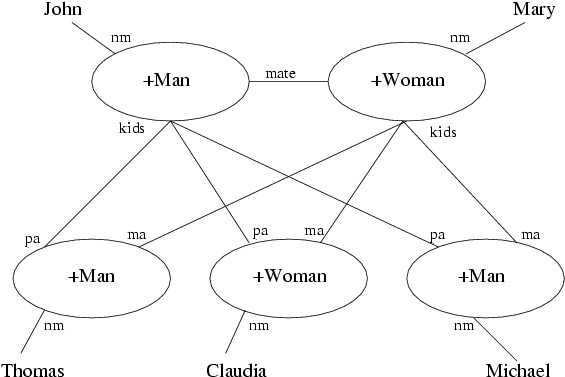
\includegraphics[scale=.5]{graphics/xmplObj.jpg}
  \caption{Family Members}
  \label{fig:family-members}
\end{figure}

In the figure, we omitted the date of birth attribute.

The bi-directional relations, connecting the parents to the children and
to each other, lend themselves to the \texttt{+Joint} entity linkage, resulting
in the following definition for a person:


\begin{wideverbatim}
(class +Person +Entity)
(rel nm   (+Key +String))          # Name
(rel pa   (+Joint) kids (+Man))    # Father
(rel ma   (+Joint) kids (+Woman))  # Mother
(rel mate (+Joint) mate (+Person)) # Partner
(rel dat  (+Date))                 # born
\end{wideverbatim}

From this base class, we can derive two classes \texttt{+Man} and \texttt{+Woman}:


\begin{wideverbatim}
(class +Man +Person)
(rel kids (+List +Joint) pa (+Person))

(class +Woman +Person)
(rel kids (+List +Joint) ma (+Person))
\end{wideverbatim}

To produce a corresponding GUI


\begin{figure}[H]
  \centering
  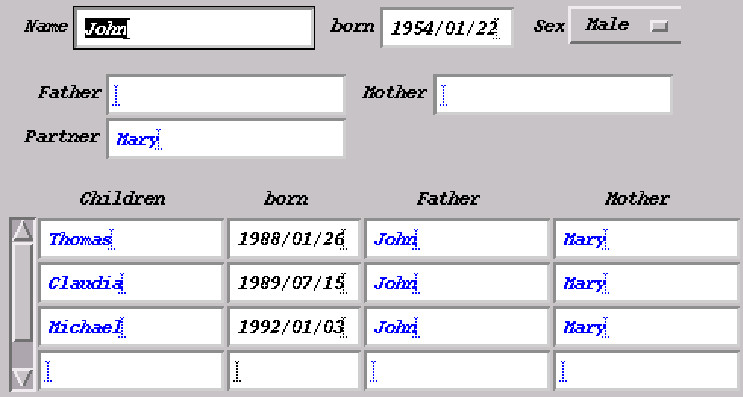
\includegraphics[scale=.5]{graphics/xmplGui.jpg}
  \caption{GUI}
  \label{fig:family-gui}
\end{figure}


allowing to view and edit the family members in the database, the
following code is sufficient:


\begin{wideverbatim}
(row
   (gui '(+E/R +TextField) '(nm : home obj) "Name" 20)
   (gui '(+E/R +DateField) '(dat : home obj) "born" 10)
   (gui '(+ClassField)
      '(: home obj) "Sex"
      '(("Male" +Man) ("Female" +Woman)) ) )
(----)
(row
   (gui '(+E/R +Obj +TextField)
      '(pa : home obj) '(nm +Man)
      "Father" 20 )
   (gui '(+E/R +Obj +TextField)
      '(ma : home obj) '(nm +Woman)
      "Mother" 20 ) )
(gui '(+E/R +Obj +TextField)
   '(mate : home obj) '(nm +Person)
   "Partner" 20 )
(---- T)

\end{wideverbatim}

\begin{wideverbatim}

(gui '(+E/R +Chart)
   '(kids : home obj)
   4 '("Children" "born" "Father" "Mother")
   (quote
      (gui '(+Obj +TextField) '(nm +Person) "" 15)
      (gui '(+Skip +Lock +DateField) "" 10)
      (gui '(+ObjView +TextField) '(: nm) "" 15)
      (gui '(+ObjView +TextField) '(: nm) "" 15) ) )
\end{wideverbatim}

The above block of code will produce exactly the layout and
functionality of the example GUI display. Without explaining all details
here, suffice it to say that the \texttt{row} function arranges the components
horizontally (while otherwise the default is vertically), \texttt{(-{}-{}-{}-)}
groups components into separate panels, and a \texttt{+Chart} creates an array
of its argument components.

The point is that this is the \emph{complete program}, not just some
important details. It specifies the whole database and GUI application.

 
\section{Discussion}
\label{sec:ul-discussion}

The previous sections and the example show that application programming
does not need to involve any concerns about database access (select,
insert, update etc.) and database integrity maintenance.

The advantages are derived from the use of prefix classes and relation
daemons. They allow to specify the complete program behavior and
appearance in a single place of definition, and in a very concise form.
Typically, the names of prefix classes are simply chained together, and
intermix freely with \texttt{Lisp}'s formal indifference of code and data.

This removes the need of maintaining separate resource files, class and
data declarations, and program code.

 
\section{Conclusion}
\label{sec:ul-conclusion}

Achieving low program development costs is an old claim. It has been
stated for manyfold methodologies and paradigms.

The system described in this paper has proven its practical value in
commercial applications during several years. Among them are sales,
accounting, report, and logistics applications. Research projects
include graphics/animation and speech synthesis systems.

This shows that it is possible to employ the concepts of prefix classes
and relation maintenance daemons successfully to commercial application
development.

We observed a significant decrease in program development time. What
used to be the major part of a project's development effort showed to
reduce to about 5 percent.

 
\section{Download}
\label{sec:ul-download}

The \texttt{PicoLisp} system can be downloaded from the
\href{http://www.software-lab.de/down.html}{PicoLisp Download}
Page~\cite{down2}.

\begin{thebibliography}{[9]}

\bibitem{allen} John Allen: ``Anatomy of Lisp'', McGraw-Hill, 1978

\bibitem{knuth} Donald E. Knuth: ``The Art of Computer Programming'',
  Vol.3, Addison-Vesley, 1973, p. 392

\bibitem{campbell}J. A. Campbell: Implementations of Prolog, Ellis Horwood Limited, 1984

\bibitem{down2} Pico Lisp Download, http://www.software-lab.de/down.html

\end{thebibliography}




%%%%%%%%%%%%%%%%%%%%%%%%%%%%%%%%%%%%%%%%%%%%%%%%%%%%%%%%%%%%%%%
% sample part title
%
% Copy it to a new file with a new name and use it
% use it as a template for your own input.
%
%%%%%%%%%%%%%%%%%%%%%%%% Springer-Verlag %%%%%%%%%%%%%%%%%%%%%%%%%%


\part{PicoLisp References}
\title{The PicoLisp Reference}
\author{Alexander Burger}
% Use \authorrunning{Short Title} for an abbreviated version of
% your contribution title if the original one is too long
\institute{\texttt{abu@software-lab.de}}
%
% Use the package "url.sty" to avoid
% problems with special characters
% used in your e-mail or web address
%


\maketitle

% \section{PicoLisp Reference}
% \label{sec:refm-picolisp-reference}

% (c) Software Lab. Alexander Burger (originally published \href{http://software-lab.de/doc/ref.html}{here}).


\begin{abstract}

This document describes the concepts, data types, and kernel functions
of the \href{http://software-lab.de/down.html}{PicoLisp} system.

This is \emph{not} a Lisp tutorial. For an introduction to Lisp, a
traditional Lisp book (like~\cite{lisp1}) is recommended. Note, however,
that there are significant differences between PicoLisp and Maclisp
(and even greater differences to Common Lisp).

Please take a look at the \emph{PicoLisp Tutorial} for an
explanation of some aspects of PicoLisp, and scan through the list of
\emph{Frequently Asked Questions (FAQ)}.

\end{abstract}  

 
\section{Introduction}
\label{sec:refm-introduction}


PicoLisp is the result of a language design study, trying to answer the
question ``What is a minimal but useful architecture for a virtual
machine?''. Because opinions differ about what is meant by ``minimal'' and
``useful'', there are many answers to that question, and people might
consider other solutions more ``minimal'' or more ``useful''. But from a
practical point of view, PicoLisp has proven to be a valuable answer to
that question.

First of all, PicoLisp is a virtual machine architecture, and then a
programming language. It was designed in a ``bottom up'' way, and ``bottom
up'' is also the most natural way to understand and to use it: \emph{Form Follows Function}.

PicoLisp has been used in several commercial and research programming
projects since 1988. Its internal structures are simple enough, allowing
an experienced programmer always to fully understand what's going on
under the hood, and its language features, efficiency and extensibility
make it suitable for almost any practical programming task.

In a nutshell, emphasis was put on four design objectives. The PicoLisp
system should be

\begin{description}

\item[Simple] The internal data structure should be as simple as
  possible. Only one single data structure is used to build all higher
  level constructs.

\item[Unlimited] There are no limits imposed upon the language due to
  limitations of the virtual machine architecture. That is, there is
  no upper bound in symbol name length, number digit counts, stack
  depth, or data structure and buffer sizes, except for the total
  memory size of the host machine.

\item[Dynamic] Behavinor should be as dynamic as possible (``run''-time
  vs. ``compile''-time). All decisions are delayed until runtime where
  possible. This involves matters like memory management, dynamic
  symbol binding, and late method binding.

\item[Practical] PicoLisp is not just a toy of theoretical value. It
  is in use since 1988 in actual application development, research and
  production.

\end{description}

\section{The PicoLisp Machine}
\label{sec:refm-the-picolisp-machine}


An important point in the PicoLisp philosophy is the knowledge about the
architecture and data structures of the internal machinery. The
high-level constructs of the programming language directly map to that
machinery, making the whole system both understandable and predictable.

This is similar to assembly language programming, where the programmer
has complete control over the machine.


 
\subsection{The Cell}
\label{sec:refm-the-cell}


The PicoLisp virtual machine is both simpler and more powerful than most
current (hardware) processors. At the lowest level, it is constructed
from a single data structure called ``cell'':


\begin{wideverbatim}
+-----+-----+
| CAR | CDR |
+-----+-----+
\end{wideverbatim}

A cell is a pair of machine words, which traditionally are called CAR
and CDR in the Lisp terminology. These words can represent either a
numeric value (scalar) or the address of another cell (pointer). All
higher level data structures are built out of cells.

The type information of higher level data is contained in the pointers
to these data. Assuming the implementation on a byte-addressed physical
machine, and a pointer size of typically 4 bytes, each cell has a size
of 8 bytes. Therefore, the pointer to a cell must point to an 8-byte
boundary, and its bit-representation will look like:


\begin{wideverbatim}
xxxxxxxxxxxxxxxxxxxxxxxxxxxxx000
\end{wideverbatim}

(the `\texttt{x}' means ``don't care''). For the individual data types, the
pointer is adjusted to point to other parts of a cell, in effect setting
some of the lower three bits to non-zero values. These bits are then
used by the interpreter to determine the data type.

In any case, bit(0) - the least significant of these bits - is reserved
as a mark bit for garbage collection.

Initially, all cells in the memory are unused (free), and linked
together to form a ``free list''. To create higher level data types at
runtime, cells are taken from that free list, and returned by the
garbage collector when they are no longer needed. All memory management
is done via that free list; there are no additional buffers, string
spaces or special memory areas, with two exceptions:

\begin{itemize}
\item A certain fixed area of memory is set aside to contain the executable
   code and global variables of the interpreter itself, and
\item a standard push down stack for return addresses and temporary
   storage. Both are not directly accessible by the programmer).
\end{itemize}


 
\subsection{Data Types}
\label{sec:refm-data-types}


On the virtual machine level, PicoLisp supports

\begin{itemize}
\item three base data types: Numbers, Symbols and Cons Pairs (Lists),
\item the three scope variations of symbols: Internal, Transient and
   External, and
\item the special symbol \texttt{NIL}.
\end{itemize}

They are all built from the single cell data structure, and all runtime
data cannot consist of any other types than these three.

The following diagram shows the complete data type hierarchy, consisting
of the three base types and the symbol variations:


\begin{wideverbatim}
                  cell
                   |
          +--------+--------+
          |        |        |
       Number    Symbol    List
                   |
                   |
 +--------+--------+--------+
 |        |        |        |
NIL   Internal Transient External
\end{wideverbatim}


\subsubsection{Numbers}
\label{sec:refm-numbers}%
A number can represent a signed integral value of arbitrary size. The
CARs of one or more cells hold the number's ``digits'' (each in the
machine's word size), to store the number's binary representation.


\begin{wideverbatim}
   Number
   |
   V
+-----+-----+
| DIG |  |  |
+-----+--+--+
         |
         V
      +-----+-----+
      | DIG |  |  |
      +-----+--+--+
               |
               V
              ...
\end{wideverbatim}

The first cell holds the least significant digit. The least significant
bit of that digit represents the sign.

The pointer to a number points into the middle of the CAR, with an
offset of 2 from the cell's start address. Therefore, the bit pattern of
a number will be:


\begin{wideverbatim}
xxxxxxxxxxxxxxxxxxxxxxxxxxxxx010
\end{wideverbatim}

Thus, a number is recognized by the interpreter when bit(1) is non-zero.


\subsubsection{Symbols}
\label{sec:refm-symbols}%
A symbol is more complex than a number. Each symbol has a value, and
optionally a name and an arbitrary number of properties. The CDR of a
symbol cell is also called VAL, and the CAR points to the symbol's tail.
As a minimum, a symbol consists of a single cell, and has no name or
properties:


\begin{wideverbatim}
      Symbol
      |
      V
+-----+-----+
|  /  | VAL |
+-----+-----+
\end{wideverbatim}

That is, the symbol's tail is empty (points to \texttt{NIL}, as indicated by
the  \texttt{/}  character).

The pointer to a symbol points to the CDR of the cell, with an offset of
4 from the cell's start address. Therefore, the bit pattern of a symbol
will be:


\begin{wideverbatim}
xxxxxxxxxxxxxxxxxxxxxxxxxxxxx100
\end{wideverbatim}

Thus, a symbol is recognized by the interpreter when bit(2) is non-zero.

A property is a key-value pair, represented as a cell in the symbol's
tail. This is called a ``property list''. The property list may be
terminated by a number representing the symbol's name. In the following
example, a symbol with the name \texttt{''abc''} has three properties: A KEY/VAL
cell, a cell with only a KEY, and another KEY/VAL cell.


\begin{wideverbatim}
      Symbol
      |
      V
+-----+-----+
|  |  | VAL |
+--+--+-----+
   | tail
   |
   V                                                      name
   +-----+-----+     +-----+-----+     +-----+-----+     +-----+-----+
   |  |  |  ---+---> | KEY |  ---+---> |  |  |  ---+---> |'cba'|  /  |
   +--+--+-----+     +-----+-----+     +--+--+-----+     +-----+-----+
      |                                   |
      V                                   V
      +-----+-----+                       +-----+-----+
      | VAL | KEY |                       | VAL | KEY |
      +-----+-----+                       +-----+-----+
\end{wideverbatim}

Each property in a symbol's tail is either a symbol (like the single KEY
above, then it represents the boolean value \texttt{T}), or a cell with the
property key in its CDR and the property value in its CAR. In both
cases, the key should be a symbol, because searches in the property list
are performed using pointer comparisons.

The name of a symbol is stored as a number at the end of the tail. It
contains the characters of the name in UTF--8 encoding, using between
one and three 8-bit-bytes per character. The first byte of the first
character is stored in the lowest 8 bits of the number.

All symbols have the above structure, but depending on scope and
accessibility there are actually four types of symbols: \texttt{NIL},
\emph{internal}, \emph{transient} and
\emph{external} symbols.


\paragraph{NIL}
\label{sec:refm-nil}%
\texttt{NIL} is a special symbol which exists exactly once in the whole system.
It is used

\begin{itemize}
\item as an end-of-list marker
\item to represent the empty list
\item to represent the boolean value ``false''
\item to represent the absolute minimum
\item to represent a string of length zero
\item to represent the value ``Not a Number''
\item as the root of all class hierarchies
\end{itemize}

For that, \texttt{NIL} has a special structure:


\begin{wideverbatim}
NIL:  /
      |
      V
+-----+-----+-----+-----+
|  /  |  /  |  /  |  /  |
+-----+--+--+-----+-----+
\end{wideverbatim}

The reason for that structure is \texttt{NIL}'s dual nature both as a symbol
and as a list:

\begin{itemize}
\item As a symbol, it should give \texttt{NIL} for its VAL, and be without
   properties
\item For the empty list, \texttt{NIL} should give \texttt{NIL} both for its CAR and for
   its CDR
\end{itemize}

These requirements are fulfilled by the above structure.

 

\paragraph{Internal Symbols}
\label{sec:refm-internal-symbols}%
Internal Symbols are all those ``normal'' symbols, as they are used for
function definitions and variable names. They are ``interned'' into an
index structure, so that it is possible to find an internal symbol by
searching for its name.

There cannot be two different internal symbols with the same name.

Initially, a new internal symbol's VAL is \texttt{NIL}.



\paragraph{Transient Symbols}
\label{sec:refm-transient-symbols}%
Transient symbols are only interned into a index structure for a certain
time (e.g. while reading the current source file), and are released
after that. That means, a transient symbol cannot be accessed then by
its name, and there may be several transient symbols in the system
having the same name.

Transient symbols are used

\begin{itemize}
\item as text strings
\item as identifiers with a limited access scope (like, for example,
   \texttt{static} identifiers in the C language family)
\item as anonymous, dynamically created objects (without a name)
\end{itemize}

Initially, a new transient symbol's VAL is that symbol itself.

A transient symbol without a name can be created with the \texttt{box} or \texttt{new}
functions.

 

\paragraph{External Symbols}
\label{sec:refm-external-symbols}%
External symbols reside in a database file (or a similar resources, see
\texttt{*Ext}), and are loaded into memory - and written back to the file -
dynamically as needed, and transparently to the programmer. They are
kept in memory (``cached'') as long as they are accessible (``referred to'')
from other parts of the program, or when they were modified but not yet
written to the database file (by \texttt{commit}).

The interpreter recognizes external symbols internally by an additional
tag bit in the tail structure.

There cannot be two different external symbols with the same name.
External symbols are maintained in index structures while they are
loaded into memory, and have their external location (disk file and
block offset) directly coded into their names (more details
\emph{here}).

Initially, a new external symbol's VAL is \texttt{NIL}, unless otherwise
specified at creation time.

 
\subsubsection{Lists}
\label{sec:refm-lists}%
A list is a sequence of one or more cells, holding numbers, symbols, or
lists.


\begin{wideverbatim}
|
V
+-----+-----+
| any |  |  |
+-----+--+--+
         |
         V
         +-----+-----+
         | any |  |  |
         +-----+--+--+
                  |
                  V
                  ...
\end{wideverbatim}

Lists are used in PicoLisp to emulate composite data structures like
arrays, trees, stacks or queues.

In contrast to lists, numbers and symbols are collectively called
``Atoms''.

Typically, the CDR of each cell in a list points to the following cell,
except for the last cell which points to \texttt{NIL}. If, however, the CDR of
the last cell points to an atom, that cell is called a ``dotted pair''
(because of its I/O syntax with a dot `\texttt{.}' between the two values).

\subsection{Memory Management}
\label{sec:refm-memory-management}


The PicoLisp interpreter has complete knowledge of all data in the
system, due to the type information associated with every pointer.
Therefore, an efficient garbage collector mechanism can easily be
implemented. PicoLisp employs a simple but fast mark-and-sweep garbage
collector.

As the collection process is very fast (in the order of milliseconds per
megabyte), it was not necessary to develop more complicated,
time-consuming and error-prone garbage collection algorithms (e.g.
incremental collection). A compacting garbage collector is also not
necessary, because the single cell data type cannot cause heap
fragmentation.

 
\section{Programming Environment}
\label{sec:refm-programming-environment}


Lisp was chosen as the programming language, because of its clear and
simple structure.

In some previous versions, a Forth-like syntax was also implemented on
top of a similar virtual machine (Lifo). Though that language was more
flexible and expressive, the traditional Lisp syntax proved easier to
handle, and the virtual machine can be kept considerably simpler.
PicoLisp inherits the major advantages of classical Lisp systems like

\begin{itemize}
\item Dynamic data types and structures
\item Formal equivalence of code and data
\item Functional programming style
\item An interactive environment
\end{itemize}

In the following, some concepts and peculiarities of the PicoLisp
language and environment are described.

 

 
\subsection{Installation}
\label{sec:refm-installation}


PicoLisp supports two installation strategies: Local and Global.

Normally, if you didn't build PicoLisp yourself but installed it with
your operating system's package manager, you will have a global
installation. This allows system-wide access to the executable and
library/documentation files.

To get a local installation, you can directly download the PicoLisp
tarball, and follow the instructions in the INSTALL file.

A local installation will not interfere in any way with the world
outside its directory. There is no need to touch any system locations,
and you don't have to be root to install it. Many different versions -
or local modifications - of PicoLisp can co-exist on a single machine.

Note that you are still free to have local installations along with a
global installation, and invoke them explicitly as desired.

Most examples in the following apply to a global installation.

 

 
\subsection{Invocation}
\label{sec:refm-invocation}


When PicoLisp is invoked from the command line, an arbitrary number of
arguments may follow the command name.

By default, each argument is the name of a file to be executed by the
interpreter. If, however, the argument's first character is a hyphen
`\texttt{-}', then the rest of that argument is taken as a Lisp function call
(without the surrounding parentheses), and a hyphen by itself as an
argument stops evaluation of the rest of the command line (it may be
processed later using the \texttt{argv} and \texttt{opt} functions). This whole
mechanism corresponds to calling \texttt{(load T)}.

A special case is if the last argument is a single `\texttt{+}'. This will
switch on debug mode (the \texttt{*Dbg} global variable) and discard the `\texttt{+}'.

As a convention, PicoLisp source files have the extension ` \texttt{.l} '.

Note that the PicoLisp executable itself does not expect or accept any
command line flags or options (except the `\texttt{+}', see above). They are
reserved for application programs.

The simplest and shortest invocation of PicoLisp does nothing, and exits
immediately by calling \texttt{bye}:


\begin{wideverbatim}
$ picolisp -bye
$
\end{wideverbatim}

In interactive mode, the PicoLisp interpreter (see \texttt{load}) will also
exit when \texttt{Ctrl-D} is entered:


\begin{wideverbatim}
$ picolisp
: $                     # Typed Ctrl-D
\end{wideverbatim}

To start up the standard PicoLisp environment, several files should be
loaded. The most commonly used things are in ``lib.l'' and in a bunch of
other files, which are in turn loaded by ``ext.l''. Thus, a typical call
would be:


\begin{wideverbatim}
$ picolisp lib.l ext.l
\end{wideverbatim}

The recommended way, however, is to call the ``pil'' shell script, which
includes ``lib.l'' and ``ext.l''. Given that your current project is loaded
by some file ``myProject.l'' and your startup function is \texttt{main}, your
invocation would look like:


\begin{wideverbatim}
$ pil myProject.l -main
\end{wideverbatim}

For interactive development it is recommended to enable debugging mode,
to get the vi-style command line editor, single-stepping, tracing and
other debugging utilities.


\begin{wideverbatim}
$ pil myProject.l -main +
\end{wideverbatim}

This is - in a local installation - equivalent to


\begin{wideverbatim}
$ ./dbg myProject.l -main
\end{wideverbatim}

or


\begin{wideverbatim}
$ ./pil myProject.l -main +
\end{wideverbatim}

In any case, the directory part of the first file name supplied
(normally, the path to ``lib.l'' as called by `pil' or `dbg') is
remembered internally as the \emph{PicoLisp Home Directory}. This path is
later automatically substituted for any leading ` \texttt{@} ' character in file
name arguments to I/O functions (see \texttt{path}).

 

 
\subsection{Input/Output}
\label{sec:refm-input/output}


In Lisp, each internal data structure has a well-defined external
representation in human-readable format. All kinds of data can be
written to a file, and restored later to their original form by reading
that file.

In normal operation, the PicoLisp interpreter continuously executes an
infinite ``read-eval-print loop''. It reads one expression at a time,
evaluates it, and prints the result to the console. Any input into the
system, like data structures and function definitions, is done in a
consistent way no matter whether it is entered at the console or read
from a file.

Comments can be embedded in the input stream with the hash \texttt{\#}
character. Everything up to the end of that line will be ignored by the
reader.


\begin{wideverbatim}
: (* 1 2 3)  # This is a comment
-> 6
\end{wideverbatim}

A comment spanning several lines may be enclosed between \texttt{\#\{} and \texttt{\}\#}.

Here is the I/O syntax for the individual PicoLisp data types (numbers,
symbols and lists) and for read-macros:

 

\subsubsection{Numbers}
\label{sec:refm-numbers}%
A number consists of an arbitrary number of digits (`\texttt{0}' through
`\texttt{9}'), optionally preceded by a sign character (`\texttt{+}' or `\texttt{-}'). Legal
number input is:


\begin{wideverbatim}
: 7
-> 7
: -12345678901245678901234567890
-> -12345678901245678901234567890
\end{wideverbatim}

Fixpoint numbers can be input by embedding a decimal point `\texttt{.}', and
setting the global variable \texttt{*Scl} appropriately:


\begin{wideverbatim}
: *Scl
-> 0

: 123.45
-> 123
: 456.78
-> 457

: (setq *Scl 3)
-> 3
: 123.45
-> 123450
: 456.78
-> 456780
\end{wideverbatim}

Thus, fixpoint input simply scales the number to an integer value
corresponding to the number of digits in \texttt{*Scl}.

Formatted output of scaled fixpoint values can be done with the \texttt{format}
and \texttt{round} functions:


\begin{wideverbatim}
: (format 1234567890 2)
-> "12345678.90"
: (format 1234567890 2 "." ",")
-> "12,345,678.90"
\end{wideverbatim}


\subsubsection{Symbols}
\label{sec:refm-symbols}%
The reader is able to recognize the individual symbol types from their
syntactic form. A symbol name should - of course - not look like a legal
number (see above).

In general, symbol names are case-sensitive. \texttt{car} is not the same as
CAR.

 
\paragraph{NIL}
\label{sec:refm-nil}%
Besides for standard normal form, \texttt{NIL} is also recognized as
\texttt{()}, \texttt{[]} or \texttt{""}.


\begin{wideverbatim}
: NIL
-> NIL
: ()
-> NIL
: ""
-> NIL
\end{wideverbatim}

Output will always appear as \texttt{NIL}.



\paragraph{Internal Symbols}
\label{sec:refm-internal-symbols}%
Internal symbol names can consist of any printable (non-whitespace)
character, except for the following meta characters:


\begin{wideverbatim}
"  '  (  )  ,  [  ]  `  ~ { }
\end{wideverbatim}

It is possible, though, to include these special characters into symbol
names by escaping them with a backslash `\textbackslash'.

The dot `\texttt{.}' has a dual nature. It is a meta character when standing
alone, denoting a \emph{dotted pair}, but can otherwise be used in
symbol names.

As a rule, anything not recognized by the reader as another data type
will be returned as an internal symbol.



\paragraph{Transient Symbols}
\label{sec:refm-transient-symbols}%
A transient symbol is anything surrounded by double quotes `\texttt{""}'. With
that, it looks - and can be used - like a string constant in other
languages. However, it is a real symbol, and may be assigned a value or
a function definition, and properties.

Initially, a transient symbol's value is that symbol itself, so that it
does not need to be quoted for evaluation:


\begin{wideverbatim}
: "This is a string"
-> "This is a string"
\end{wideverbatim}

However, care must be taken when assigning a value to a transient
symbol. This may cause unexpected behavior:


\begin{wideverbatim}
: (setq "This is a string" 12345)
-> 12345
: "This is a string"
-> 12345
\end{wideverbatim}

The name of a transient symbol can contain any character except the
null-byte. A double quote character can be escaped with a backslash
`\textbackslash', and a backslash itself has to be escaped with another backslash.
Control characters can be written with a preceding hat `\texttt{\^}' character.

\begin{wideverbatim}
: "We^Ird\\Str\"ing"
-> "We^Ird\\Str\"ing"
: (chop @)
-> ("W" "e" "^I" "r" "d" "\\" "S" "t" "r" "\"" "i" "n" "g")
\end{wideverbatim}

The index for transient symbols is cleared automatically before and
after  \texttt{load}ing a source file, or it can be reset explicitly with the \texttt{====} function. With that mechanism, it is possible to create symbolsb
with a local access scope, not accessible from other parts of the
program.

A special case of transient symbols are \emph{anonymous symbols}. These are
symbols without name (see \texttt{box}, \texttt{box?} or \texttt{new}). They print as a
dollar sign (\texttt{\$}) followed by a decimal digit string (actually their
machine address).


\paragraph{External Symbols}
\label{sec:refm-external-symbols}%
External symbol names are surrounded by braces (`\texttt{{}' and `\texttt{}}'). The
characters of the symbol's name itself identify the physical location of
the external object. This is

\begin{itemize}
\item in the 32-bit version: The number of the database file, and -
   separated by a hyphen - the starting block in the database file. Both
   numbers are encoded in base--64 notation (characters `\texttt{0}' through
   `\texttt{9}', `\texttt{:}', `\texttt{;}', `\texttt{A}' through `\texttt{Z}' and `\texttt{a}' through `\texttt{z}').
\item in the 64-bit version: The number of the database file minus 1 in
   ``hax'' notation (i.e. hexadecimal/alpha notation, where  \texttt{@}  is zero,
   `\texttt{A}' is 1 and  \texttt{O}  is 15 (from ``alpha'' to ``omega'')), immediately
   followed (without a hyphen) the starting block in octal (`\texttt{0}'
   through `\texttt{7}').
\end{itemize}

In both cases, the database file (and possibly the hypen) are omitted
for the first (default) file.

 
\subsubsection{Lists}
\label{sec:refm-lists}%
Lists are surrounded by parentheses ( \texttt{(}  and  \texttt{)} ).

\texttt{(A)} is a list consisting of a single cell, with the symbol \texttt{A} in its
CAR, and \texttt{NIL} in its CDR.

\texttt{(A B C)} is a list consisting of three cells, with the symbols \texttt{A}, \texttt{B}
and \texttt{C} respectively in their CAR, and \texttt{NIL} in the last cell's CDR.

\texttt{(A . B)} is a ``dotted pair'', a list consisting of a single cell, with
the symbol \texttt{A} in its CAR, and \texttt{B} in its CDR.

PicoLisp has built-in support for reading and printing simple circular
lists. If the dot in a dotted-pair notation is immediately followed by a
closing parenthesis, it indicates that the CDR of the last cell points
back to the beginning of that list.


\begin{wideverbatim}
: (let L '(a b c) (conc L L))
-> (a b c .)
: (cdr '(a b c .))
-> (b c a .)
: (cddddr '(a b c .))
-> (b c a .)
\end{wideverbatim}

A similar result can be achieved with the function \texttt{circ}. Such lists
must be used with care, because many functions won't terminate or will
crash when given such a list.

\subsubsection{Read-Macros}
\label{sec:refm-read-macros}%
Read-macros in PicoLisp are special forms that are recognized by the
reader, and modify its behavior. Note that they take effect immediately
while  \texttt{read}ing an expression, and are not seen by the \texttt{eval} in the
main loop.

The most prominent read-macro in Lisp is the single quote character \texttt{'} 
which expands to a call of the \texttt{quote} function. Note that the single
quote character is also printed instead of the full function name.


\begin{wideverbatim}
: '(a b c)
-> (a b c)
: '(quote . a)
-> 'a
: (cons 'quote 'a)   # (quote . a)
-> 'a
: (list 'quote 'a)   # (quote a)
-> '(a)
\end{wideverbatim}

A comma  \texttt{,}  will cause the reader to collect the following data item
into an \texttt{idx} tree in the global variable \texttt{*Uni}, and to return a
previously inserted equal item if present. This makes it possible to
create a unique list of references to data which do normally not follow
the rules of pointer equality. If the value of \texttt{*Uni} is \texttt{T}, the comma
read macro mechanism is disabled.

A single backquote character \texttt{`} will cause the reader to evaluate the
following expression, and return the result.


\begin{wideverbatim}
: '(a `(+ 1 2 3) z)
-> (a 6 z)
\end{wideverbatim}

A tilde character \texttt{\textasciitilde{}} inside a list will cause the reader to evaluate
the following expression, and (destructively) splice the result into the
list.


\begin{wideverbatim}
: '(a b c ~(list 'd 'e 'f) g h i)
-> (a b c d e f g h i)
\end{wideverbatim}

When a tilde character is used to separate two symbol names (without
surrounding whitespace), the first is taken as a namespace to look up
the second (64-bit version only).


\begin{wideverbatim}
: 'libA~foo  # Look up 'foo' in namespace 'libA'
-> "foo"     # "foo" is not interned in the current namespace
\end{wideverbatim}

Reading \texttt{libA\textasciitilde{}foo} is equivalent to switching the current namespace to
\texttt{libA} (with \texttt{symbols}), reading the symbol \texttt{foo}, and then switching
back to the original namespace.

Brackets (`\texttt{[}' and `\texttt{]}') can be used as super parentheses. A closing
bracket will match the innermost opening bracket, or all currently open
parentheses.


\begin{wideverbatim}
: '(a (b (c (d]
-> (a (b (c (d))))
: '(a (b [c (d]))
-> (a (b (c (d))))
\end{wideverbatim}

Finally, reading the sequence `\texttt{{}}' will result in a new anonymous
symbol with value \texttt{NIL}, equivalent to a call to \texttt{box} without
arguments.


\begin{wideverbatim}
: '({} {} {})
-> ($134599965 $134599967 $134599969)
: (mapcar val @)
-> (NIL NIL NIL)
\end{wideverbatim}

\subsection{Evaluation}
\label{sec:refm-evaluation}


PicoLisp tries to evaluate any expression encountered in the
read-eval-print loop. Basically, it does so by applying the following
three rules:

\begin{itemize}
\item A number evaluates to itself.
\item A symbol evaluates to its value (VAL).
\item A list is evaluated as a function call, with the CAR as the function
   and the CDR the arguments to that function. These arguments are in
   turn evaluated according to these three rules.
\end{itemize}


\begin{wideverbatim}
: 1234
-> 1234        # Number evaluates to itself
: *Pid
-> 22972       # Symbol evaluates to its VAL
: (+ 1 2 3)
-> 6           # List is evaluated as a function call
\end{wideverbatim}

For the third rule, however, things get a bit more involved. First - as
a special case - if the CAR of the list is a number, the whole list is
returned as it is:


\begin{wideverbatim}
: (1 2 3 4 5 6)
-> (1 2 3 4 5 6)
\end{wideverbatim}

This is not really a function call but just a convenience to avoid
having to quote simple data lists.

Otherwise, if the CAR is a symbol or a list, PicoLisp tries to obtain an
executable function from that, by either using the symbol's value, or by
evaluating the list.

What is an executable function? Or, said in another way, what can be
applied to a list of arguments, to result in a function call? A legal
function in PicoLisp is either a

\begin{description}
\item[number] When a number is used as a function, it is simply taken as a
pointer to executable code that will be called with the list of
(unevaluated) arguments as its single parameter. It is up to that code
to evaluate the arguments, or not. Some functions do not evaluate their
arguments (e.g. \texttt{quote}) or evaluate only some of their arguments (e.g.
\texttt{setq}). 
\end{description}

or a 

\begin{description}
 \item[lambda expression] A lambda expression is a list, whose CAR is
either a symbol or a list of symbols, and whose CDR is a list of
expressions. Note: In contrast to other Lisp implementations, the symbol
LAMBDA itself does not exist in PicoLisp but is implied from context.

A few examples should help to understand the practical consequences of
these rules. In the most common case, the CAR will be a symbol defined
as a function, like the \texttt{*} in:
\end{description}

\begin{wideverbatim}
: (* 1 2 3)    # Call the function '*'
-> 6
\end{wideverbatim}

Inspecting the VAL of \texttt{*} gives


\begin{wideverbatim}
: *            # Get the VAL of the symbol '*'
-> 67318096
\end{wideverbatim}

The VAL of \texttt{*} is a number. In fact, it is the numeric representation of
a C-function pointer, i.e. a pointer to executable code. This is the
case for all built-in functions of PicoLisp.

Other functions in turn are written as Lisp expressions:


\begin{wideverbatim}
: (de foo (X Y)            # Define the function 'foo'
   (* (+ X Y) (+ X Y)) )
-> foo
: (foo 2 3)                # Call the function 'foo'
-> 25
: foo                      # Get the VAL of the symbol 'foo'
-> ((X Y) (* (+ X Y) (+ X Y)))
\end{wideverbatim}

The VAL of \texttt{foo} is a list. It is the list that was assigned to \texttt{foo}
with the \texttt{de} function. It would be perfectly legal to use \texttt{setq}
instead of \texttt{de}:


\begin{wideverbatim}
: (setq foo '((X Y) (* (+ X Y) (+ X Y))))
-> ((X Y) (* (+ X Y) (+ X Y)))
: (foo 2 3)
-> 25
\end{wideverbatim}

If the VAL of \texttt{foo} were another symbol, that symbol's VAL would be used
instead to search for an executable function.

As we said above, if the CAR of the evaluated expression is not a symbol
but a list, that list is evaluated to obtain an executable function.


\begin{wideverbatim}
: ((intern (pack "c" "a" "r")) (1 2 3))
-> 1
\end{wideverbatim}

Here, the \texttt{intern} function returns the symbol \texttt{car} whose VAL is used
then. It is also legal, though quite dangerous, to use the code-pointer
directly:


\begin{wideverbatim}
: *
-> 67318096
: ((* 2 33659048) 1 2 3)
-> 6
: ((quote . 67318096) 1 2 3)
-> 6
: ((quote . 1234) (1 2 3))
Segmentation fault
\end{wideverbatim}

When an executable function is defined in Lisp itself, we call it a
\emph{lambda expression}. A lambda expression always has a list of executable
expressions as its CDR. The CAR, however, must be a either a list of
symbols, or a single symbol, and it controls the evaluation of the
arguments to the executable function according to the following rules:


\begin{description}
\item[When the CAR is a list of symbols] For each of these symbols an
  argument is evaluated, then the symbols are bound simultaneously to
  the results. The body of the lambda expression is executed, then the
  VAL's of the symbols are restored to their original values. This is
  the most common case, a fixed number of arguments is passed to the
  function.
\item[Otherwise, when the CAR is the symbol \texttt{@}] All arguments
  are evaluated and the results kept internally in a list. The body of
  the lambda expression is executed, and the evaluated arguments can
  be accessed sequentially with the \texttt{args}, \texttt{next},
  \texttt{arg} and \texttt{rest} functions. This allows to define
  functions with a variable number of evaluated arguments.
\item[Otherwise, when the CAR is a single symbol] The symbol is bound
  to the whole unevaluated argument list. The body of the lambda
  expression is executed, then the symbol is restored to its original
  value. This allows to define functions with unevaluated arguments.
  Any kind of interpretation and evaluation of the argument list can
  be done inside the expression body.
\end{description}

In all cases, the return value is the result of the last expression in
the body.

\begin{wideverbatim}
: (de foo (X Y Z)                   # CAR is a list of symbols
   (list X Y Z) )                   # Return a list of all arguments
-> foo
: (foo (+ 1 2) (+ 3 4) (+ 5 6))
-> (3 7 11)                         # all arguments are evaluated
\end{wideverbatim}


\begin{wideverbatim}
: (de foo X                         # CAR is a single symbol
   X )                              # Return the argument
-> foo
: (foo (+ 1 2) (+ 3 4) (+ 5 6))
-> ((+ 1 2) (+ 3 4) (+ 5 6))        # the whole unevaluated list is returned
\end{wideverbatim}


\begin{wideverbatim}
: (de foo @                         # CAR is the symbol '@'
   (list (next) (next) (next)) )    # Return the first three arguments
-> foo
: (foo (+ 1 2) (+ 3 4) (+ 5 6))
-> (3 7 11)                         # all arguments are evaluated
\end{wideverbatim}

Note that these forms can also be combined. For example, to evaluate
only the first two arguments, bind the results to \texttt{X} and \texttt{Y}, and bind
all other arguments (unevaluated) to \texttt{Z}:


\begin{wideverbatim}
: (de foo (X Y . Z)                 # CAR is a list with a dotted-pair tail
   (list X Y Z) )                   # Return a list of all arguments
-> foo
: (foo (+ 1 2) (+ 3 4) (+ 5 6))
-> (3 7 ((+ 5 6)))                  # Only the first two arguments are evaluated
\end{wideverbatim}

Or, a single argument followed by a variable number of arguments:


\begin{wideverbatim}
: (de foo (X . @)                   # CAR is a dotted-pair with '@'
   (println X)                      # print the first evaluated argument
   (while (args)                    # while there are more arguments
      (println (next)) ) )          # print the next one
-> foo
: (foo (+ 1 2) (+ 3 4) (+ 5 6))
3                                   # X
7                                   # next argument
11                                  # and the last argument
-> 11
\end{wideverbatim}

In general, if more than the expected number of arguments is supplied to
a function, these extra arguments will be ignored. Missing arguments
default to \texttt{NIL}.

 

 
\subsection{Coroutines}
\label{sec:refm-coroutines}


Coroutines are independent execution contexts. They may have multiple
entry and exit points, and preserve their environment between
invocations.

They are available only in the 64-bit version.

A coroutine is identified by a tag. This tag can be passed to other
functions, and (re)invoked as needed. In this regard coroutines are
similar to ``continuations'' in other languages.

When the tag goes out of scope while it is not actively running, the
coroutine will be garabage collected. In cases where this is desired,
using a \emph{transient} symbol for the tag is recommended.

A coroutine is created by calling \texttt{co}. Its \texttt{prg} body will be executed,
and unless \texttt{yield} is called at some point, the coroutine will ``fall
off'' at the end and disappear.

When \texttt{yield} is called, control is either transferred back to the
caller, or to some other - explicitly specified, and already running -
coroutine.

A coroutine is stopped and disposed when

\begin{itemize}
\item execution falls off the end
\item some other (co)routine calls \texttt{co} with that tag but without a \texttt{prg}
   body
\item a \texttt{throw} into another (co)routine environment is executed
\item an error occurred, and \emph{error handling} was entered
\end{itemize}

In the current implementation, not more than 64 coroutines can exist at
the same time. Reentrant coroutines are not supported, a coroutine
cannot resume itself directly or indirectly.

 

 
\subsection{Interrupt}
\label{sec:refm-interrupt}


During the evaluation of an expression, the PicoLisp interpreter can be
interrupted at any time by hitting \texttt{Ctrl-C}. It will then enter the
breakpoint routine, as if \texttt{!} were called.

Hitting ENTER at that point will continue evaluation, while \texttt{(quit)}
will abort evaluation and return the interpreter to the top level. See
also \texttt{debug}, \texttt{e}, \texttt{\textasciicircum{}} and \texttt{*Dbg}

Other interrupts may be handled by \texttt{alarm}, \texttt{sigio}, \texttt{*Hup} and
\texttt{*Sig[12]}.

 

 
\subsection{Error Handling}
\label{sec:refm-error-handling}


When a runtime error occurs, execution is stopped and an error handler
is entered.

The error handler resets the I/O channels to the console, and displays
the location (if possible) and the reason of the error, followed by an
error message. That message is also stored in the global \texttt{*Msg}, and the
location of the error in \texttt{\textasciicircum{}}. If the VAL of the global \texttt{*Err} is
non-\texttt{NIL} it is executed as a \texttt{prg} body. If the standard input is from
a terminal, a read-eval-print loop (with a question mark ` \texttt{?} ' as
prompt) is entered (the loop is exited when an empty line is input).
Then all pending \texttt{finally} expressions are executed, all variable
bindings restored, and all files closed. If the standard input is not
from a terminal, the interpreter terminates. Otherwise it is reset to
its top-level state.


\begin{wideverbatim}
: (de foo (A B) (badFoo A B))       # 'foo' calls an undefined symbol
-> foo
: (foo 3 4)                         # Call 'foo'
!? (badFoo A B)                     # Error handler entered
badFoo -- Undefined
? A                                 # Inspect 'A'
-> 3
? B                                 # Inspect 'B'
-> 4
?                                   # Empty line: Exit
:
\end{wideverbatim}

Errors can be caught with \texttt{catch}, if a list of substrings of possible
error messages is supplied for the first argument. In such a case, the
matching substring (or the whole error message if the substring is
\texttt{NIL}) is returned.

An arbitrary error can be thrown explicitly with \texttt{quit}.

 

 
\subsection{@ Result}
\label{sec:refm-@-result}


In certain situations, the result of the last evaluation is stored in
the VAL of the symbol \texttt{@}. This can be very convenient, because it often
makes the assignment to temporary variables unnecessary.

This happens in two - only superficially similar - situations:

\begin{description}
\item[load] In read-eval loops, the last three results which were
  printed at the console are available in \texttt{@@@}, \texttt{@@}
  and~\texttt{@}, in that order (i.e the latest result is
  in~\texttt{@}).

\begin{wideverbatim}
: (+ 1 2 3)
-> 6
: (/ 128 4)
-> 32
: (- @ @@)        # Subtract the last two results
-> 26
\end{wideverbatim}

\item[Flow functions] Flow- and logic-functions store the result of
  their controlling expression - respectively non-\texttt{NIL} results
  of their conditional expression - in~\texttt{@}.

\begin{wideverbatim}
: (while (read) (println 'got: @))
abc            # User input
got: abc       # print result
123            # User input
got: 123       # print result
NIL
-> 123

: (setq L (1 2 3 4 5 1 2 3 4 5))
-> (1 2 3 4 5 1 2 3 4 5)
: (and (member 3 L) (member 3 (cdr @)) (set @ 999))
-> 999
: L
-> (1 2 3 4 5 1 2 999 4 5)
\end{wideverbatim}

Functions with controlling expressions are \emph{case},
\emph{prog1}, \emph{prog2}, and the bodies
of \texttt{*Run} tasks.

Functions with conditional expressions are \emph{and},
\emph{cond}, \emph{do}, \emph{for},
\emph{if}, \emph{if2}, \emph{ifn},
\emph{loop}, \emph{nand},
\emph{nond}, \emph{nor},
\emph{not}, \emph{or},
\emph{state}, \emph{unless},
\emph{until}, \emph{when} and
\emph{while}.

\end{description}

\texttt{@} is generally local to functions and methods, its value is
automatically saved upon function entry and restored at exit.

\subsection{Comparing}
\label{sec:refm-comparing}


In PicoLisp, it is legal to compare data items of arbitrary type. Any
two items are either

\begin{description}
\item[Identical] They are the same memory object (pointer equality).
  For example, two internal symbols with the same name are identical.
  In the 64-bit version, also short numbers (up to 60 bits plus sign)
  are pointer-equal.
\item[Equal] They are equal in every respect (structure equality), but
  need not to be identical. Examples are numbers with the same value,
  transient symbols with the same name or lists with equal elements.
\item[Or they have a well-defined ordinal relationship] Numbers are
  comparable by their numeric value, strings by their name, and lists
  recursively by their elements (if the CAR's are equal, their CDR's
  are compared). For differing types, the following rule applies:
  Numbers are less than symbols, and symbols are less than lists. As
  special cases, \texttt{NIL} is always less than anything else, and
  \texttt{T} is always greater than anything else.
\end{description}

To demonstrate this, \texttt{sort} a list of mixed data types:

\begin{wideverbatim}
: (sort '("abc" T (d e f) NIL 123 DEF))
-> (NIL 123 DEF "abc" (d e f) T)
\end{wideverbatim}

See also \texttt{max}, \texttt{min}, \texttt{rank}, \texttt{<}, \texttt{=}  \texttt{>} etc.

 
\subsection{OO Concepts}
\label{sec:refm-oo-concepts}

PicoLisp comes with built-in object oriented extensions. There seems to
be a common agreement upon three criteria for object orientation:

\begin{description}
\item[Encapsulation] Code and data are encapsulated into objects,
  giving them both a behavior and a state. Objects communicate by
  sending and receiving messages.
\item[Inheritance] Objects are organized into classes. The behavior of
  an object is inherited from its class(es) and superclass(es).
\item[Polymorphism] Objects of different classes may behave
  differently in response to the same message. For that, classes may
  define different methods for each message.
\end{description}

PicoLisp implements both objects and classes with symbols. Object-local
data are stored in the symbol's property list, while the code (methods)
and links to the superclasses are stored in the symbol's VAL
(encapsulation).

In fact, there is no formal difference between objects and classes
(except that objects usually are anonymous symbols containing mostly
local data, while classes are named internal symbols with an emphasis on
method definitions). At any time, a class may be assigned its own local
data (class variables), and any object can receive individual method
definitions in addition to (or overriding) those inherited from its
(super)classes.

PicoLisp supports multiple inheritance. The VAL of each object is a
(possibly empty) association list of message symbols and method bodies,
concatenated with a list of classes. When a message is sent to an
object, it is searched in the object's own method list, and then (with a
left-to-right depth-first search) in the tree of its classes and
superclasses. The first method found is executed and the search stops.
The search may be explicitly continued with the \texttt{extra} and \texttt{super}
functions.

Thus, which method is actually executed when a message is sent to an
object depends on the classes that the object is currently linked to
(polymorphism). As the method search is fully dynamic (late binding), an
object's type (i.e. its classes and method definitions) can be changed
even at runtime!

While a method body is being executed, the global variable \texttt{This} is set
to the current object, allowing the use of the short-cut property
functions \texttt{\texttt{}}, \texttt{:} and \texttt{::}.

 

 
\subsection{Database}
\label{sec:refm-database}


On the lowest level, a PicoLisp database is just a collection of
\emph{external symbols}. They reside in a database file, and are
dynamically swapped in and out of memory. Only one database can be open
at a time (\texttt{pool}).

In addition, further external symbols can be specified to originate from
arbitrary sources via the \texttt{*Ext} mechanism.

Whenever an external symbol's value or property list is accessed, it
will be automatically fetched into memory, and can then be used like any
other symbol. Modifications will be written to disk only when \texttt{commit}
is called. Alternatively, all modifications since the last call to
\texttt{commit} can be discarded by calling \texttt{rollback}.

\subsubsection{Transactions}
\label{sec:refm-transactions}%
In the typical case there will be multiple processes operating on the
same database. These processes should be all children of the same parent
process, which takes care of synchronizing read/write operations and
heap contents. Then a database transaction is normally initiated by
calling \texttt{(dbSync)}, and closed by calling \texttt{(commit 'upd)}. Short
transactions, involving only a single DB operation, are available in
functions like \texttt{new!} and methods like \texttt{put!>} (by convention with an
exclamation mark), which implicitly call \texttt{(dbSync)} and \texttt{(commit 'upd)}
themselves.

A transaction proceeds through five phases:

\begin{enumerate}
\item \texttt{dbSync} waits to get a \texttt{lock} on the root object \texttt{*DB}. Other
   processes continue reading and writing meanwhile.
\item \texttt{dbSync} calls \texttt{sync} to synchronize with changes from other
   processes. We hold the shared lock, but other processes may continue
   reading.
\item We make modifications to the internal state of external symbols with
   \texttt{put>, set>, lose>} etc. We - and also other processes - can still
   read the DB.
\item We call \texttt{(commit 'upd)}. \texttt{commit} obtains an exclusive lock (no more
   read operations by other processes), writes an optional transaction
   log, and then all modified symbols. As \texttt{upd} is passed to `commit',
   other processes synchronize with these changes.
\item Finally, all locks are released by `commit'
\end{enumerate}


 
\subsubsection{Entities / Relations}
\label{sec:refm-entities-/-relations}%
The symbols in a database can be used to store arbitrary information
structures. In typical use, some symbols represent nodes of search
trees, by holding keys, values, and links to subtrees in their VAL's.
Such a search tree in the database is called index.

For the most part, other symbols in the database are objects derived
from the \texttt{+Entity} class.

Entities depend on objects of the \texttt{+relation} class hierarchy.
Relation-objects manage the property values of entities, they define the
application database model and are responsible for the integrity of
mutual object references and index trees.

Relations are stored as properties in the entity classes, their methods
are invoked as daemons whenever property values in an entity are
changed. When defining an \texttt{+Entity} class, relations are defined - in
addition to the method definitions of a normal class - with the \texttt{rel}
function. Predefined relation classes include

\begin{itemize}
\item Primitive types like
   \texttt{+Symbol}
   Symbolic data
   \texttt{+String}
   Strings (just a general case of symbols)
   \texttt{+Number}
   Integers and fixpoint numbers
   \texttt{+Date}
   Calendar date values, represented by a number
   \texttt{+Time}
   Time-of-the-day values, represented by a number
   \texttt{+Blob}
   ``Binary large objects'' stored in separate files
\item Object-to-object relations
   \texttt{+Link}
   A reference to some other entity
   \texttt{+Hook}
   A reference to an entity holding object-local index trees
   \texttt{+Joint}
   A bi-directional reference to some other entity
\item Container prefix classes like
   \texttt{+List}
   A list of any of the other primitive or object relation types
   \texttt{+Bag}
   A list containing a mixture of any of the other types
\item Index prefix classes
   \texttt{+Ref}
   An index with other primitives or entities as key
   \texttt{+Key}
   A unique index with other primitives or entities as key
   \texttt{+Idx}
   A full-text index, typically for strings
   \texttt{+Sn}
   Tolerant index, using a modified Soundex-Algorithm
\item Booleans
   \texttt{+Bool}
   \texttt{T} or \texttt{NIL}
\item And a catch-all class
   \texttt{+Any}
   Not specified, may be any of the above relations
\end{itemize}


\subsection{Pilog (PicoLisp Prolog)}
\label{sec:refm-pilog-(picolisp-prolog)}


A declarative language is built on top of PicoLisp, that has the
semantics of Prolog, but uses the syntax of Lisp.

For an explanation of Prolog's declarative programming style, an
introduction like~\cite{prolog1} is recommended.

Facts and rules can be declared with the \texttt{be} function. For example, a
Prolog fact `\texttt{likes(john,mary).}' is written in Pilog as:


\begin{wideverbatim}
(be likes (John Mary))
\end{wideverbatim}

and a rule `\texttt{likes(john,X) :- likes(X,wine), likes(X,food).}' is in
Pilog:


\begin{wideverbatim}
(be likes (John @X) (likes @X wine) (likes @X food))
\end{wideverbatim}

As in Prolog, the difference between facts and rules is that the latter
ones have conditions, and usually contain variables.

A variable in Pilog is any symbol starting with an at-mark character
(` \texttt{@} '). The symbol \texttt{@} itself can be used as an anonymous variable: It
will match during unification, but will not be bound to the matched
values.

The \emph{cut} operator of Prolog (usually written as an exclamation mark
(\texttt{!})) is the symbol \texttt{T} in Pilog.

An interactive query can be done with the \texttt{?} function:


\begin{wideverbatim}
(? (likes John @X))
\end{wideverbatim}

This will print all solutions, waiting for user input after each line.
If a non-empty line (not just a ENTER key, but for example a dot (\texttt{.})
followed by ENTER) is typed, it will terminate.

Pilog can be called from Lisp and vice versa:

\begin{itemize}
\item The interface from Lisp is via the functions \texttt{goal} (prepare a query
   from Lisp data) and \texttt{prove} (return an association list of successful
   bindings), and the application level functions \texttt{pilog} and \texttt{solve}.
\item When the CAR of a Pilog clause is a Pilog variable, the CDR is
   executed as a Lisp expression and the result unified with that
   variable.
\item Within such a Lisp expression in a Pilog clause, the current bindings
   of Pilog variables can be accessed with the \texttt{->} function.
\end{itemize}

\subsection{Naming Conventions}
\label{sec:refm-naming-conventions}


It was necessary to introduce - and adhere to - a set of conventions for
PicoLisp symbol names. Because all (internal) symbols have a global
scope (there are no packages or name spaces), and each symbol can only
have either a value or function definition, it would otherwise be very
easy to introduce name conflicts. Besides this, source code readability
is increased when the scope of a symbol is indicated by its name.

These conventions are not hard-coded into the language, but should be so
into the head of the programmer. Here are the most commonly used ones:

\begin{itemize}
\item Global variables start with an asterisk ``\texttt{*}''
\item Functions and other global symbols start with a lower case letter
\item Locally bound symbols start with an upper case letter
\item Local functions start with an underscore `` \texttt{\_}''
\item Classes start with a plus-sign ``\texttt{+}'', where the first letter
\begin{itemize}
\item is in lower case for abstract classes
\item and in upper case for normal classes
\end{itemize}
\item Methods end with a right arrow ``\texttt{>}''
\item Class variables may be indicated by an upper case letter
\end{itemize}

For historical reasons, the global constant symbols \texttt{T} and \texttt{NIL} do not
obey these rules, and are written in upper case.

For example, a local variable could easily overshadow a function
definition:


\begin{wideverbatim}
: (de max-speed (car)
   (.. (get car 'speeds) ..) )
-> max-speed
\end{wideverbatim}

Inside the body of \texttt{max-speed} (and all other functions called during
that execution) the kernel function \texttt{car} is redefined to some other
value, and will surely crash if something like \texttt{(car Lst)} is executed.
Instead, it is safe to write:


\begin{wideverbatim}
: (de max-speed (Car)            # 'Car' with upper case first letter
   (.. (get Car 'speeds) ..) )
-> max-speed
\end{wideverbatim}

Note that there are also some strict naming rules (as opposed to the
voluntary conventions) that are required by the corresponding kernel
functionalities, like:

\begin{itemize}
\item Transient symbols are enclosed in double quotes (see
   \emph{Transient Symbols})
\item External symbols are enclosed in braces (see \emph{External Symbols})
\item Pattern-Wildcards start with an at-mark ` \texttt{@} ' (see
   \emph{match} and \emph{fill})
\item Symbols referring to a shared library contain a colon ` \texttt{lib:sym} '
\end{itemize}

With that, the last of the above conventions (local functions start with
an underscore) is not really necessary, because true local scope can be
enforced with transient symbols.

 
\subsection{Breaking Traditions}
\label{sec:refm-breaking-traditions}


PicoLisp does not try very hard to be compatible with traditional Lisp
systems. If you are used to some other Lisp dialects, you may notice the
following differences:

\begin{description}

\item[Case Sensitivity] PicoLisp distinguishes between upper case and
  lower case characters in symbol names. Thus, \texttt{CAR} and
  \texttt{car} are different symbols, which was not the case in
  traditional Lisp systems.

\item[QUOTE] In traditional Lisp, the \texttt{QUOTE} function
  returns its \emph{first} unevaluated argument. In PicoLisp, on the
  other hand, \texttt{quote} returns \emph{all} (unevaluated)
  argument(s).

\item[LAMBDA] The \texttt{LAMBDA} function, in some way at
  the heart of traditional Lisp, is completely missing (and
  \texttt{quote} is used instead).

\item[PROG] The \texttt{PROG} function of traditional Lisp,
  with its GOTO and ENTER functionality, is also missing. PicoLisp's
  \texttt{prog} function is just a simple sequencer (as \texttt{PROGN}
  in some Lisps).

\item[Function/Value] In PicoLisp, a symbol cannot have a value
  \emph{and} a function definition at the same time. Though this is a
  disadvantage at first sight, it allows a completely uniform handling
  of functional data.

\end{description} 

\subsection{Bugs}
\label{sec:refm-bugs}


The names of the symbols \texttt{T} and \texttt{NIL} violate the \emph{naming conventions}. They are global symbols, and should therefore start with
an asterisk ``\texttt{*}''. It is too easy to bind them to some other value by
mistake:


\begin{wideverbatim}
(de foo (R S T)
   ...
\end{wideverbatim}

However, \texttt{lint} will issue a warning in such a case.

\begin{thebibliography}{[9]}

\bibitem{lisp1} Winston/Horn: ``Lisp'', Addison-Wesley, 1981

\bibitem{prolog1} Clocksin/Mellish: ``Programming in Prolog'',
  Springer-Verlag, 1981

\end{thebibliography}

\title{The Equivalence of Code and Data}
\author{Alexander Burger}
% Use \authorrunning{Short Title} for an abbreviated version of
% your contribution title if the original one is too long
\institute{\texttt{abu@software-lab.de}}
%
% Use the package "url.sty" to avoid
% problems with special characters
% used in your e-mail or web address
%


\maketitle

% % 16jul12
% % Alexander Burger

% \documentclass[10pt,a4paper]{article}
% \usepackage{graphicx}

% \textwidth 1.4\textwidth
% \textheight 1.125\textheight
% \oddsidemargin 0em
% \evensidemargin 0em
% \headsep 0em
% \parindent 0em
% \parskip 6pt

% \title{The Equivalence of Code and Data}
% \author{Alexander Burger\\abu@software-lab.de}
% \date{2011-07-29}

% \begin{document}
% \maketitle

\begin{abstract}
  This article demonstrates how the \emph{equivalence of code and
    data}, as a powerful abstraction instrument, supports the
  ``locality principle of structure, content and behavior'' in PicoLisp.
\end{abstract}

\section{The Equivalence of Code and Data}
\label{sec:equiv-equivalence-code-data}

Why does PicoLisp make so much fuss about that equivalence of code and data?
Answer: Because it is such a powerful abstraction instrument! It supports the
``locality principle of structure, content and behavior''.

Let me try to explain this using a GUI example, though the same principle also
applies to most other libraries and applications. Take a simple GUI page:
\begin{wideverbatim}
   (action
      (html 0 "Increment" "lib.css" NIL
         (form NIL
            (gui '(+Var +NumField) '*Num 9)
            (gui '(+JS +Button) "+" '(inc '*Num)) ) ) )
\end{wideverbatim}

This page shows two components, a numeric input field and a button labeled ``+``.
You can either enter a value into that field, or increment its value with the
button.

The page has a \textit{structure}, namely a HTML body containing a form, which in turn
contains the two components. It has \textit{content}, the numeric value shown in the
field. And it has \textit{behavior}, as the numeric field handles string conversion
and error checking, and the button increments the number.

Note that a fourth attribute of the page, the \textit{layout and style}, is not
discussed here. It is maintained separately in the CSS file.

The three attributes structure, content and behavior, however, cannot be
separated. This may be contrary to some schools of thought, which advocate a
separation of structure and content, and behavior anyway. But obviously the HTML
structure also holds content like the ``Increment'' page title or the ``+`` button
label. And this content might also be subject to behavior, for example the
button label may change dynamically:
\begin{wideverbatim}
   (gui '(+JS +Button)
      (if *VerboseDisplay "Increment" "+")
      '(inc '*Num) )
\end{wideverbatim}

Or the button may prompt a confirmation dialog to the user:
\begin{wideverbatim}
   (gui '(+JS +Button) "+"
      '(ask "Increment value?"
         (inc '*Num) ) )
\end{wideverbatim}

The equivalence of code and data makes the development of functions like
\texttt{html}, \texttt{form}, \texttt{gui} or \texttt{ask} particularly simple. The list
\begin{wideverbatim}
   (ask "Increment value?" (inc '*Num))
\end{wideverbatim}

is \textit{data} for the \texttt{gui} function. \texttt{gui} constructs a component of the class
\texttt{+Button}, and simply stows away that list into the new component. Later, when
the button is pressed, it is executed. It is just that simple.

\texttt{gui} itself doesn't understand anything about buttons and what they do with
these arguments. It is all data. From the view of the button, however, that list
is a piece of code, to be executed when the button is pressed.

Later, when \texttt{ask} is executed, the situation is similar. A dialog is shown
which displays the question ``Increment value?'', and a ``Yes'' and a ``No'' button.
The ``Yes'' button receives the expression \texttt{(inc '*Num)}, to increment the number
when pressed.

The example can be modified, to operate on database entities instead. Instead of
connecting the numeric field to a variable (with the \texttt{+Var} prefix class), we
connect it to the \texttt{count} property of the database object, and instead of
incrementing the variable, the button increments that object's count attribute:
\begin{wideverbatim}
   (gui '(+E/R +NumField) '(count : home obj) 9)
   (gui '(+JS +Button) "+" '(inc!> (: home obj) 'count))
\end{wideverbatim}

No need to write some separate database ``select'' or ``update'' functionality! It
is all in a single place.

This shows how easily any kind of application logic can be implemented using
this style. In a typical application hundreds or thousands of such components
are put together, so it is essential that this can be done with as little noise
and redundancy as possible.

This becomes especially evident if you compare this style with the GUI and
application strategies of other languages, for example in the RosettaCode
tasks
\underline{GUI component interaction}\footnote{http://rosettacode.org/wiki/GUI\_component\_interaction\#PicoLisp}
and
\underline{GUI enabling/disabling of controls}\footnote{http://rosettacode.org/wiki/GUI\_enabling/disabling\_of\_controls\#PicoLisp}.

In other environments, you usually end up defining constants, components and
functions in separate locations. This is the opposite of what PicoLisp
advocates, the ``locality principle of structure, content and behavior''.



\title{First Class Environments}
\author{Alexander Burger}
% Use \authorrunning{Short Title} for an abbreviated version of
% your contribution title if the original one is too long
\institute{\texttt{abu@software-lab.de}}
%
% Use the package "url.sty" to avoid
% problems with special characters
% used in your e-mail or web address
%


\maketitle

% 16jul12
% Alexander Burger

% \documentclass[10pt,a4paper]{article}
% \usepackage{graphicx}

% \textwidth 1.4\textwidth
% \textheight 1.125\textheight
% \oddsidemargin 0em
% \evensidemargin 0em
% \headsep 0em
% \parindent 0em
% \parskip 6pt

% \title{First Class Environments}
% \author{Alexander Burger\\abu@software-lab.de}
% \date{2012-05-24}

% \begin{document}
% \maketitle

\begin{abstract}
  This article discusses the advantages and technical details of
  \emph{first class environments} in PicoLisp. First, the differences
  between \emph{dynamic binding} and \emph{lexical scoping} are
  highlighted, then \emph{first class data types} and \emph{first
    class environments} are discussed. 
\end{abstract}


\section{Dynamic Binding vs Lexical Scoping}
\label{sec:firstclass-dynamic-binding}

PicoLisp uses dynamic binding for symbolic variables. This means that
the value of a symbol is determined by the current runtime context,
not by the lexical context in the source file.

This has advantages in practical programming. It allows you to write
independent code fragments as \textbf{data} which can be passed to
other parts of the program to be later executed as \textbf{code} in
that context.

For example, the major part of the PicoLisp GUI framework consists of
code snippets, which are installed as event handlers, button actions
or update managers in GUI components.

In a lexically scoped language, you can't separate code from its
environment. A call like \texttt{(foo X Y)} has no meaning by itself
(unless \texttt{X} and \texttt{Y} are treated as ``free'' variables,
i.e. dynamically, not lexically). Instead, you must write a
\texttt{let} or \texttt{lambda} expression, or pass around full
function definitions as closures. All this is much more noisy
(consider the typical case of dozens of such fragments in a single GUI
page).

PicoLisp tries to be as dynamic as possible. This involves also (and
much more important than just variable bindings) things like
I/O-channels,
'\underline{make}\footnote{http://software-lab.de/doc/refM.html\#make}'
environments, the place of the currently executed method in the
inheritance hierarchy (for
'\underline{super}\footnote{http://software-lab.de/doc/refS.html\#super}'
and
'\underline{extra}\footnote{http://software-lab.de/doc/refE.html\#extra}')
or the current
'\underline{This}\footnote{http://software-lab.de/doc/refT.html\#This}'
object. A running code fragment can always assume to have access to
these environments.

This article is only concerned about variable bindings.

\section{First Class Data Type}
\label{sec:firstclass-first-class-data-type}

In programming languages, a first class data type can be created and manipulated
separately within the language, independent from its intended purpose.

For a \textbf{function}, for example, the intended purpose is to \textit{call} it. If it is
a first class function, it can be build, passed around etc., independent from
that. The two tasks (creating and calling the function) can be handled
independently within the language.

For an \textbf{environment}, the intended purpose is to
\begin{enumerate}
   \item activate it
   \item execute one or more expressions in it
   \item deactivate it, possibly restoring the previous environment
\end{enumerate}
If it is a first class environment it, can also be created and manipulated
within the language.

\section{First Class Environments}
\label{sec:firstclass-first-class-environments}

To make such an environment useful, it is important that the three tasks
(creation, activation/deactivation and execution) can be controlled
independently.

Let us consider the expression \texttt{(foo X Y)} again. Assume we want to execute it
in an environment where \texttt{X} is 3 and \texttt{Y} is 4. The direct way is
\begin{wideverbatim}
   (let (X 3 Y 4)
      (foo X Y) )
\end{wideverbatim}

This handles the three tasks all at once. It creates and activates the
environment, immediately executes the code, and then deactivates the
environment.

If the expression \texttt{(foo X Y)} is supplied from the application code,
stand-alone in one part of the application, and is supposed to run in some other
part of the application in an environment active there at that moment, it is
also no problem. It can simply be executed:
\begin{wideverbatim}
   (foo X Y)
\end{wideverbatim}

If, however, that application environment supposed to be manipulated
separately, for example because it is passed over across a HTTP transaction or
appears in an RPC call, then the
\begin{itemize}
   \item creation of that environment is typically done in the application
   \item activation of that environment is done in the GUI framework
   \item execution of the expression(s) is done in the application
   \item deactivation is done in the GUI framework again
\end{itemize}

\subsection{Creation}
\label{sec:firstclass-creation}

The environment is represented by a list of symbol-value pairs. It can be
created with the direct, explicit lisp operations, or more conveniently with the
'\underline{env}\footnote{http://software-lab.de/doc/refE.html\#env}' function.

If the environment is intended as a subset of the current environment, i.e. if
you simply want to create it with the current values of \texttt{X} and \texttt{Y}, you may
write
\begin{wideverbatim}
   : (setq Env (env '(X Y)))
   -> ((Y . 4) (X . 3))
\end{wideverbatim}

Otherwise, you may pass explit values
\begin{wideverbatim}
   : (setq Env (env 'X 3 'Y 4))
   -> ((Y . 4) (X . 3))
\end{wideverbatim}


\subsection{Activation}
\label{sec:firstclass-activation}

The simplest way to activate an environment would be to to iterate over the list
and '\underline{set}\footnote{http://software-lab.de/doc/refS.html\#set}' each symbol to its value.
This is normally not recommended, because it would not restore the previous
environment when done.

In most cases either '\underline{bind}\footnote{http://software-lab.de/doc/refB.html\#bind}' or
'\underline{job}\footnote{http://software-lab.de/doc/refJ.html\#job}' are used. The main difference
between these two functions is that job modifies the environment destructively,
to store modified values before restoring the previous environment.
\begin{wideverbatim}
   : (bind Env (* X Y))
   -> 12

   : (job Env (* X Y))
   -> 12
\end{wideverbatim}

If the environment is to be modified by the expression, use 'job':
\begin{wideverbatim}
   : Env
   -> ((Y . 4) (X . 3))

   : (job Env (* X (inc 'Y)))
   -> 15

   : Env
   -> ((Y . 5) (X . 3))
\end{wideverbatim}

These examples don't show the separation of activation and execution, as this
cannot be simply done in an isolated example. For a real-world use case, take a
look at the top-level GUI function in ``@lib/form.l``. The relevant part can be
reduced to
\begin{wideverbatim}
   (with "*App"                        # Point 'This' to the current form
      (job (: env)                     # Activate environment of that form
         (<post> ...
            (<hidden> ...)
            ...
            (if *PRG
               (let gui
                  ...
                  (htPrin "Prg") )     # Execute the GUI code
               ...
               (let gui
                  ...
                  (htPrin "Prg") )     # Execute the GUI code
\end{wideverbatim}

The GUI code which actually builds the page is in \texttt{"Prg"}. When it runs,
\texttt{This} and the desired environment (from the form's \texttt{env} property) are
properly activated.

A similar case can be found more down in ``@lib/form.l`` in 'postGui' to handle
HTTP POST and XMLHttpRequest events.

\title{Even small details make a difference!}
\author{Alexander Burger}
% Use \authorrunning{Short Title} for an abbreviated version of
% your contribution title if the original one is too long
\institute{\texttt{abu@software-lab.de}}
%
% Use the package "url.sty" to avoid
% problems with special characters
% used in your e-mail or web address
%


\maketitle


% 16jul12
% Alexander Burger

% \documentclass[10pt,a4paper]{article}
% \usepackage{graphicx}

% \textwidth 1.4\textwidth
% \textheight 1.125\textheight
% \oddsidemargin 0em
% \evensidemargin 0em
% \headsep 0em
% \parindent 0em
% \parskip 6pt

% \title{Even small details make a difference!}
% \author{Alexander Burger\\abu@software-lab.de}
% \date{2011-07-29}

% \begin{document}
% \maketitle

\begin{abstract}
  This article discusses how it's unique implementation of the
  \texttt{quote} function makes PicoLisp more efficient than other
  Lisp's in terms of both space and time. 
\end{abstract}

\section{Even small details make a difference!}
\label{sec:quote-small-details}

In Lisp, the single quote character plays a central role. It is actually a
\textit{read macro}, which expands to the built-in function \texttt{quote}. Its purpose is
to inhibit the evaluation of the following argument, and \texttt{quote} is one of the
most often called functions.

But it is remarkable that almost all Lisp implementations handle this in a
somewhat suboptimal way. They define \texttt{quote} to return its \textit{first} argument,
without evaluating it. So far so good. But when you think about that for a
moment, you may ask: ``Why only the first argument?''

This is inefficient, both in terms of space and time, and has no benefit at all.
Yet almost all Lisp implementations stick to it.

PicoLisp breaks with that bad habit, and defines \texttt{quote} to return \textit{all}
arguments, without evaluating them.

Let's look at some examples: Quoted expressions like
\begin{wideverbatim}
   'a
   '(a b)
   '(a . x)
\end{wideverbatim}

expand in traditional Lisps to
\begin{wideverbatim}
   (quote a)
   (quote (a b))
   (quote (a . x))
\end{wideverbatim}

while in PicoLisp, they expand to
\begin{wideverbatim}
   (quote . a)
   (quote a b)
   (quote a . x)
\end{wideverbatim}

This makes quite a difference, as it uses only half the space (two cells in
traditional Lisp, but only one in PicoLisp):
\begin{wideverbatim}
   (quote a)
      +-------+-------+      +-------+-------+
      | quote |   ----+----> |   a   |  NIL  |
      +-------+-------+      +-------+-------+

   (quote . a)
      +-------+-------+
      | quote |   a   |
      +-------+-------+
\end{wideverbatim}

\begin{wideverbatim}
   (quote (a b))
      +-------+-------+      +-------+-------+
      | quote |   ----+----> |   |   |  NIL  |
      +-------+-------+      +---+---+-------+
                                 |
                                 V
                             +-------+-------+      +-------+-------+
                             |   a   |   ----+----> |   b   |  NIL  |
                             +-------+-------+      +-------+-------+

   (quote a b)
      +-------+-------+      +-------+-------+      +-------+-------+
      | quote |   ----+----> |   a   |   ----+----> |   b   |  NIL  |
      +-------+-------+      +-------+-------+      +-------+-------+
\end{wideverbatim}

\begin{wideverbatim}
   (quote (a . x))
      +-------+-------+      +-------+-------+
      | quote |   ----+----> |   |   |  NIL  |
      +-------+-------+      +---+---+-------+
                                 |
                                 V
                             +-------+-------+
                             |   a   |   x   |
                             +-------+-------+

   (quote a . x)
      +-------+-------+      +-------+-------+
      | quote |   ----+----> |   a   |   x   |
      +-------+-------+      +-------+-------+
\end{wideverbatim}

The runtime code for a traditional \texttt{quote} has more work to do. It needs two
pointer dereferences to get the data, while PicoLisp needs only one.

For that reason, \texttt{quote} is the shortest of all functions in PicoLisp, being
\begin{wideverbatim}
   any doQuote(any x) {return cdr(x);}
\end{wideverbatim}

in \texttt{C}, or
\begin{wideverbatim}
   (code 'doQuote 2)
      ld E (E CDR)  # Get CDR
      ret
\end{wideverbatim}

in \texttt{asm}.



\title{The Dual Nature of NIL}
\author{Alexander Burger}
% Use \authorrunning{Short Title} for an abbreviated version of
% your contribution title if the original one is too long
\institute{\texttt{abu@software-lab.de}}
%
% Use the package "url.sty" to avoid
% problems with special characters
% used in your e-mail or web address
%


\maketitle

% 16jul12
% Alexander Burger

% \documentclass[10pt,a4paper]{article}
% \usepackage{graphicx}

% \textwidth 1.4\textwidth
% \textheight 1.125\textheight
% \oddsidemargin 0em
% \evensidemargin 0em
% \headsep 0em
% \parindent 0em
% \parskip 6pt

% \title{The Dual Nature of NIL}
% \author{Alexander Burger\\abu@software-lab.de}
% \date{2012-06-07}

% \begin{document}
% \maketitle

\begin{abstract}
  In this article, the dual nature of \texttt{NIL} as symbol and cons
  pair, a basic design requirement of PicoLisp, is discussed. 
\end{abstract}

\section{The Dual Nature of NIL}
\label{sec:dual-nature-nil}

\texttt{NIL} is a very fundamental piece of data. It has a dual
nature, being both a symbol \textit{and} a cons pair of the form
\texttt{(NIL . NIL)}. From the beginning, this has been a basic design
requirement of PicoLisp.

As shown in ``doc64/structures`` (similar also in ''doc/structures``):

\begin{wideverbatim}
      NIL:  /
            |
            V
      +-----+-----+-----+-----+
      |'LIN'|  /  |  /  |  /  |
      +-----+--+--+-----+-----+
\end{wideverbatim}

Physically, the pointer to \texttt{NIL} (shown with the 'V' in the
above diagram) is a true symbol, as it points at an offset of a
pointer size into the memory heap. Taken as such, \texttt{NIL} is a
normal symbol,

\begin{wideverbatim}
      NIL:  /
            |
            V
      +-----+-----+
      |'LIN'|  /  |
      +-----+--+--+
\end{wideverbatim}

having a tail with the characters 'N', 'I' and 'L' (the name), and a
value which in turn points to \texttt{NIL} (symbolized with the '/').

However, when this pointer is boldly used as a cell pointer (by
ignoring the pointer tags caused by the pointer size offset)

\begin{wideverbatim}
      NIL:  /
            |
            V
            +-----+-----+
            |  /  |  /  |
            +--+--+-----+
\end{wideverbatim}

then it is a normal cons pair, with \texttt{NIL} in its CAR and
\texttt{NIL} in its CDR, which just happens to be misaligned in memory
(i.e. at the place of a symbol).

This structure has great advantages. Any proper list (ending with
\texttt{NIL}) becomes sort of ``infinite'', allowing to take the CDR
as often as possible and still obtain \texttt{NIL} again and again.

Therefore, a function doesn't need to check whether it actually
received an argument or not. It can simply take the next argument with
CDR from the argument list, and doesn't see any difference between
\texttt{(foo NIL)} and \texttt{(foo)}. This makes interpretation both
simpler and faster.


% Local variables:
% mode: latex
% TeX-master: "../../editor.tex"
% End:

\title{Array Abstinence}
\author{Alexander Burger}
% Use \authorrunning{Short Title} for an abbreviated version of
% your contribution title if the original one is too long
\institute{\texttt{abu@software-lab.de}}
%
% Use the package "url.sty" to avoid
% problems with special characters
% used in your e-mail or web address
%


\maketitle

% 16jul12
% Alexander Burger

% \documentclass[10pt,a4paper]{article}
% \usepackage{graphicx}

% \textwidth 1.4\textwidth
% \textheight 1.125\textheight
% \oddsidemargin 0em
% \evensidemargin 0em
% \headsep 0em
% \parindent 0em
% \parskip 6pt

% \title{Array Abstinence}
% \author{Alexander Burger\\abu@software-lab.de}
% \date{2011-07-29}

% \begin{document}
% \maketitle

\begin{abstract}
  The differences between lists and arrays as well as the question if
  arrays are really needed are discussed, followed by relative
  performance considerations. 
\end{abstract}

\section{Introduction}
\label{sec:array-abst-introduction}

Some people are unhappy with the situation that PicoLisp has no
built-in array (or vector) data type. As described in the reference
manual, the \underline{PicoLisp
  Machine}\footnote{http://software-lab.de/doc/ref.html\#vm} supports
exactly \underline{three data
  types}\footnote{http://software-lab.de/doc/ref.html\#data}: Numbers,
Symbols and Lists.

But what about arrays? After all, any other language supports arrays! We are so
very much used to them.

If we look at a typical Fortran, C or Java program, we find almost every second
statement to be something like (e.g. in Java):
\begin{wideverbatim}
   for (i = 0; i < Arr.length; ++i)
      doSomething(Arr[i]);
\end{wideverbatim}

It is nearly impossible to survive in such languages without arrays.

\section{What is an Array?}
\label{sec:array-abst-what-is-an-array?}

An array is a wonderful data structure.

It implements a mapping of numeric keys (integers) to arbitrary data. Given a
number, the associated data can be found in O(1) time. And the keys themselves
do not take up any memory space, they exist implicit in the data offsets form
the array's start address.

\section{Lists}
\label{sec:array-abst-lists}

PicoLisp has lists.

A list can simulate an array, albeit less efficiently. It takes up twice the
space, and indexed access to its data takes O(N/2) time on the average.

But lists have a lot of advantages, and are also more efficient than arrays in
many other cases. We do not need to discuss these advantages here in detail, any
Lisp programmer will know them.

As PicoLisp strives for simplicity, there is no room for an additional data type
- also for hard physical reasons, as the number of precious tag bits is limited.
To fully support an array data type, all those powerful built-in list
manipulation functions would need array counterparts, and the programmer would
permanently need to make design decisions whether to use lists or arrays for the
problem at hand.

If there is a choice between arrays \textbf{or} lists, lists will clearly win.

\section{Are Arrays \textit{Really} Needed?}
\label{sec:array-abst-are-arrays-really-needed}

My short answer would be ``No''. The advantages in efficiency do not outweigh the
disadvantages of increased complexity.

I would even say that the proponents of arrays in PicoLisp misunderstand some
aspects of PicoLisp programming.

The predominance of arrays in other languages, as shown with the above example
\begin{wideverbatim}
   for (i = 0; i < Arr.length; ++i)
      doSomething(Arr[i]);
\end{wideverbatim}

does not carry over to PicoLisp. Such constructs are simply not used. Instead,
you have a large number of mapping functions at your disposal:
\begin{wideverbatim}
   (mapc doSomething Arr)
\end{wideverbatim}

In fact, it is the lack of functionality for the direct manipulation of compound
data, which requires the excess indexing into arrays in other languages.

The mistake is mixing up two separate concepts:
\begin{enumerate}
   \item Sequential access to certain pieces of data
   \item Mapping integer keys to data items
\end{enumerate}
What arrays are \textit{really} needed for is point (2): You have an integer, and want
to get the corresponding piece of data.

Point (1), however, can and should be handled directly and elegantly with
mapping and other access functions.

So back to point (2). \textit{When} in our programming life do we really need to map
integers to data?

These cases are surprisingly rare. We have to keep in mind that for arrays only
the mapping of continuous integer ranges makes sense. Most practical tasks of
mapping numbers to other data involve sparse or non-linear input data, or
non-integers, or no numeric keys at all.

Sure, there are typical cases like image rasterization. But when did you the
last time implement Bresenham's line algorithm in \textit{application} programming?
Instead, you resort to a library, or write it in C or even assembly if a library
is not available.

In other cases - like two-dimensional maps - there are better ways. Look for
example how the board in the PicoLisp chess program (and other games and many
rosetta code solutions) is implemented with direct connection attributes (north,
west etc.) between the fields instead of integer arithmetics for array indexes.

For more flexible (not only integer, or even numeric) key mapping, built-in
mechanisms like association lists, symbol properties or binary
'\underline{idx}\footnote{http://software-lab.de/doc/refI.html\#idx}' trees can be used. Agreed,
these mechanisms are less efficient than simple integer-indexed arrays, but the
difference is not very dramatic.

\section{Relative Performance Consideration}
\label{sec:array-abst-relative-performance-consideration}

What would be the performance penalty for using lists instead of arrays, if we
would really need a mapping of a continuous integer range to other data?

Let's assume an integer array of length 100, initialized to increasing values:
\begin{wideverbatim}
   int Arr[100];

   for (i = 0; i < 100; ++i)
      Arr[i] = i;
\end{wideverbatim}

In PicoLisp, this is equivalent to
\begin{wideverbatim}
   (setq List (range 1 100))
\end{wideverbatim}


Now let's increment each element:
\begin{wideverbatim}
   for (i = 0; i < 100; ++i)
      ++Arr[i];
\end{wideverbatim}

The PicoLisp version would be
\begin{wideverbatim}
   (map inc List)
\end{wideverbatim}

but let's assume for a moment we have no mapping function, and insist on
indexed access instead:
\begin{wideverbatim}
   (for N 100
      (inc (nth List N)) )
\end{wideverbatim}

'\underline{nth}\footnote{http://software-lab.de/doc/refN.html\#nth}' is PicoLisp's idea of an
indexed array access.

Let's compare that to an analog O(1) access, by repeatedly accessing the
first list element:
\begin{wideverbatim}
   (for N 100
      (inc (nth List 1)) )
\end{wideverbatim}

The time difference will be the relative overhead for the O(N/2) access to
indexed list elements.

To get measurable timing results, we do each test ten thousand times. First the
accesses to all list elements:
\begin{wideverbatim}
   : (bench
      (do 10000
         (for N 100
            (inc (nth List N)) ) ) )
   0.282 sec
\end{wideverbatim}


Then the ``simulation of an array data type'', by accessing only the first
element:
\begin{wideverbatim}
   : (bench
      (do 10000
         (for N 100
            (inc (nth List 1)) ) ) )
   0.121 sec
\end{wideverbatim}


We can see, the results are in the same order of magnitude. The difference of
161 milliseconds was the time actually spent in list traversals.

In fact, the greatest part of execution time is taken by the interpreter
overhead anyway. Compare this to a full-list increment using
'\underline{map}\footnote{http://software-lab.de/doc/refM.html\#map}':
\begin{wideverbatim}
   : (bench
      (do 10000
         (map inc List) ) )
   0.076 sec
\end{wideverbatim}

Of course the difference gets bigger if the list gets longer, but typically
there will be also much more processing of the data than simple increments.

Regarding all that, it should become clear that wasting tag bits and efforts for
such a data type and its associated functions is not a good idea.

\title{Coroutines}
\author{Alexander Burger}
% Use \authorrunning{Short Title} for an abbreviated version of
% your contribution title if the original one is too long
\institute{\texttt{abu@software-lab.de}}
%
% Use the package "url.sty" to avoid
% problems with special characters
% used in your e-mail or web address
%


\maketitle

% 16jul12
% Alexander Burger

% \documentclass[10pt,a4paper]{article}
% \usepackage{graphicx}

% \textwidth 1.4\textwidth
% \textheight 1.125\textheight
% \oddsidemargin 0em
% \evensidemargin 0em
% \headsep 0em
% \parindent 0em
% \parskip 6pt

% \title{Coroutines}
% \author{Alexander Burger\\abu@software-lab.de}
% \date{2011-07-29}

% \begin{document}
% \maketitle


\begin{abstract}
This article introduces application examples for \emph{coroutines},
comparing their use and relative efficiency with a possible solution
via \emph{generators}.     
\end{abstract}

\section{Introduction}
\label{sec:coroutines-introduction}

With picoLisp-3.0.3, the 64-bit version of PicoLisp has support for
\underline{coroutines}\footnote{http://software-lab.de/doc/ref.html\#coroutines}. This article tries
to show their basic usage.

Assume we need all Pythagorean triples (i.e. all numbers A, B and C, such that
% A\char942 + B\char942 = C\char942)
$A + B = C$  with elements between 1 and N. A straightforward way to print
them is:
\begin{wideverbatim}
   (de pythag (N)
      (for A N
         (for B (range A N)
            (for C (range B N)
               (when (= (+ (* A A) (* B B)) (* C C))
                  (println (list A B C)) ) ) ) ) )
\end{wideverbatim}

We get:
\begin{wideverbatim}
   : (pythag 20)
   (3 4 5)
   (5 12 13)
   (6 8 10)
   (8 15 17)
   (9 12 15)
   (12 16 20)
\end{wideverbatim}

However, just printing the triples is not very useful if they were needed in
various situations for further processing. The lispy way for a general tool is
passing a \textit{function} to \texttt{pythag} and decide later what to do with the data:
\begin{wideverbatim}
   (de pythag (N Fun)
      (for A N
         (for B (range A N)
            (for C (range B N)
               (when (= (+ (* A A) (* B B)) (* C C))
                  (Fun (list A B C)) ) ) ) ) )
\end{wideverbatim}

(note that for a truly general tool, we would write \texttt{Fun} and the local
variables as transient symbols to avoid conflicts)

Now we can print them again
\begin{wideverbatim}
   : (pythag 20 println)
   (3 4 5)
   (5 12 13)
   (6 8 10)
   (8 15 17)
   (9 12 15)
   (12 16 20)
\end{wideverbatim}

collect them into a list if we like
\begin{wideverbatim}
   : (make (pythag 20 link))
   -> ((3 4 5) (5 12 13) (6 8 10) (8 15 17) (9 12 15) (12 16 20))
\end{wideverbatim}

or do with them whatever we like.

Still, this method has its limits. What if we need to pass a very large number
for \texttt{N}, and we want to access the values one by one, perhaps in the course of
some other involved calculation? Pre-generating the list of all values might not
be feasible.

\section{Using a Generator}
\label{sec:coroutines-using-a-generator}

One way to solve this problem is a generator. This function returns the next
value each time it is called:
\begin{wideverbatim}
   (de pythag (N)
      (job '((A . 1) (B . 1) (C . 0))
         (loop
            (when (> (inc 'C) N)
               (when (> (inc 'B) N)
                  (setq B (inc 'A)) )
               (setq C B) )
            (T (> A N))
            (T (= (+ (* A A) (* B B)) (* C C))
               (list A B C) ) ) ) )

   : (pythag 20)
   -> (3 4 5)
   : (pythag 20)
   -> (5 12 13)
   : (pythag 20)
   -> (6 8 10)
   ...
\end{wideverbatim}

Now we can call it whenever we need a new value. The function encapsulates the
state of its local variables in a \underline{job}\footnote{http://software-lab.de/doc/refJ.html\#job} environment.

A major disadvantage, however, is that it does not reflect the flow of control.
The three nested \texttt{for} loops above had to be unfolded and programmed manually.
This is hard to read, even for this simple case, and may be difficult or
impossible to program in more complicated cases.

\section{Using a Coroutine}
\label{sec:coroutines-using-a-coroutine}

A coroutine preserves the local environment, as well as the state of control of
a function. It may have multiple exit points, and continue execution where it
left off the last time.

This is done via two new functions: \underline{co}\footnote{http://software-lab.de/doc/refC.html\#co} and \underline{yield}\footnote{http://software-lab.de/doc/refY.html\#yield}.
\begin{wideverbatim}
   (de pythag (N)
      (co 'pythag
         (for A N
            (for B (range A N)
               (for C (range B N)
                  (when (= (+ (* A A) (* B B)) (* C C))
                     (yield (list A B C)) ) ) ) ) ) )

   : (pythag 20)
   -> (3 4 5)
   : (pythag 20)
   -> (5 12 13)
   : (pythag 20)
   -> (6 8 10)
   ...
\end{wideverbatim}

So this is a generator equivalent to the one above, but with cleanly nested
\texttt{for} loops.

The function \texttt{co} is called with a \textbf{tag} argument, and an executable \textbf{body}
(a \textit{prg}), similar to \underline{catch}\footnote{http://software-lab.de/doc/refC.html\#catch}. When
called the first time, a new coroutine for that tag is created, and the body
gets executed. If called again later, and an existing coroutine for that tag is
found, execution will continue at the point where it left off last time with
\texttt{yield}.

\texttt{yield} stops executing the coroutine's body, and immediately returns to the
caller (or to some other coroutine if desired). When a coroutine is resumed with
\texttt{co}, it will continue at the point of the last call to \texttt{yield}. If it is
resumed by a call to \texttt{yield} in another coroutine, the return value of the
first \texttt{yield} is the value given as an argument to the second \texttt{yield}.

\section{Efficiency}
\label{sec:coroutines-efficiency}

In terms of memory usage, coroutines are rather expensive, because each of them
requires its own stack segment. For that reason (and also due to internal
structures) the maximum number of coroutines in the system is limited to 64.

To my surprise, however, coroutines are quite efficient in terms of runtime
overhead. Measuring the context switch to and from an empty coroutine (an
endless loop with just a (yield))
\begin{wideverbatim}
   : (bench (do 1000000 (co 'bench (loop (yield)))))
   0.380 sec
   -> NIL
\end{wideverbatim}

shows that it needs just 0.38 / 2 = 0.19 microseconds per switch operation.

This is in the same order of magnitude of a normal function call:
\begin{wideverbatim}
   : (bench (do 1000000 ((quote (X Y) (+ X Y)) 3 4)))
   0.162 sec
   -> 7
\end{wideverbatim}

Comparing the implementations of \texttt{pythag} above - as a generator using \texttt{job}
and a coroutine - shows that the coroutine version is about 10 percent faster.

\section{Inspecting and Stopping Coroutines}
\label{sec:coroutines-inspecting-and-stopping-coroutines}

The function \underline{stack}\footnote{http://software-lab.de/doc/refS.html\#stack} can be used to
see which coroutines are currently running (in addition to its primary task of
setting or returning the current stack segment size).

Let's say we called \texttt{pythag} like in the example above, and then started two
more coroutines as
\begin{wideverbatim}
   : (co "routine1" (yield 1))
   -> 1
   : (co "routine2" (yield 2))
   -> 2
\end{wideverbatim}

Now there must be three coroutines running. \texttt{stack} returns them:
\begin{wideverbatim}
   : (stack)
   -> ("routine2" "routine1" pythag . 4)
\end{wideverbatim}


When \texttt{co} is called with only a \texttt{tag}, but without a body, the corresponding
coroutine is stopped.
\begin{wideverbatim}
   : (co "routine1")
   -> T
   : (co "routine2")
   -> T
   : (co 'pythag)
   -> T
   : (stack)
   -> 4
\end{wideverbatim}

Now all coroutines are gone, and \texttt{stack} returns only the remaining segment
size (in megabytes).

\section{A Tree Example}
\label{sec:coroutines-a-tree-example}

A typical example of a situation where a coroutine can simplify things a lot, is
a recursive algorithm.

For testing, let's generate a balanced binary tree:
\begin{wideverbatim}
   (balance '*Tree (range 1 15))
\end{wideverbatim}

As you may know, you can display it with the
\underline{view}\footnote{http://software-lab.de/doc/refV.html\#view} function
\begin{wideverbatim}
   : (view *Tree T)
            15
         14
            13
      12
            11
         10
            9
   8
            7
         6
            5
      4
            3
         2
            1
\end{wideverbatim}

It is easy to traverse such a tree, e.g. to print its nodes:
\begin{wideverbatim}
   : (de printNodes (Tree)
      (when Tree
         (printNodes (cadr Tree))
         (println (car Tree))
         (printNodes (cddr Tree)) ) )
   -> printNodes

   : (printNodes *Tree)
   1
   2
   3
   4
   5
   6
   7
   8
   9
   10
   11
   12
   13
   14
   15
\end{wideverbatim}

But what if you want to get the nodes returned, one by one, as in a generator
function? For example, to compare the nodes of two trees and see of they are
equal? If you think about it, you'll see that it is not trivial.

With a coroutine, it is straightforward. We can write a function that returns
another node upon each call:
\begin{wideverbatim}
   (de nextLeaf (Rt Tree)
      (co Rt
         (recur (Tree)
            (when Tree
               (recurse (cadr Tree))
               (yield (car Tree))
               (recurse (cddr Tree)) ) ) ) )
\end{wideverbatim}

With that, we can write a function to compare two trees
\begin{wideverbatim}
   (de cmpTrees (Tree1 Tree2)
      (prog1
         (use (Node1 Node2)
            (loop
               (setq
                  Node1 (nextLeaf "rt1" Tree1)
                  Node2 (nextLeaf "rt2" Tree2) )
               (T (nor Node1 Node2) T)
               (NIL (= Node1 Node2)) ) )
         (co "rt1")
         (co "rt2") ) )
\end{wideverbatim}

The last two calls to \texttt{co} stop the two coroutines, independent of the result.


\title{Transient Namespaces}
\author{Alexander Burger}
% Use \authorrunning{Short Title} for an abbreviated version of
% your contribution title if the original one is too long
\institute{\texttt{abu@software-lab.de}}
%
% Use the package "url.sty" to avoid
% problems with special characters
% used in your e-mail or web address
%


\maketitle

\begin{abstract}
  This articles is about using use a transient symbol (instead of an
  internal symbol) for a \textit{temporary} namespace.
\end{abstract}


\section{Introduction}
\label{sec:transient-namespaces-introduction}

A few days ago I hit upon an interesting concept: Transient Namespaces.

With Transient Namespaces I do not mean namespaces for transient symbols (there
is always only one single namespace for transient symbols at any moment), but to
use a transient symbol (instead of an internal symbol) for a \textit{temporary}
namespace.

It turns out that this makes quite some sense.

\section{Using transient symbols}
\label{sec:transient-namespaces-using-transient-symbols}

Last week I added an example for the Common-Lisp-style \texttt{DO*} function to
\underline{macros}\footnote{http://software-lab.de/doc/faq.html\#macros}
\begin{verbatim}
   (de do* "Args"
      (bind (mapcar car (car "Args"))
         (for "A" (car "Args")
            (set (car "A") (eval (cadr "A"))) )
         (until (eval (caadr "Args"))
            (run (cddr "Args"))
            (for "A" (car "Args")
               (and (cddr "A") (set (car "A") (run @))) ) )
         (run (cdadr "Args")) ) )
\end{verbatim}

It can be used as
\begin{verbatim}
   : (do* ((A 123) (B 'abc) (C 1 (inc C)))
      ((> C 7) (pack A B))
      (println C) )
   1
   2
   3
   4
   5
   6
   7
   -> "123abc"
\end{verbatim}

As you see, the above implementation of \texttt{do*} uses \textit{transient} symbols for
\texttt{"A"} and \texttt{"Args"}. This is the recommended way, to avoid symbol conflicts
(``captures'' in CL-terminology).

\section{Using internal symbols}
\label{sec:transient-namespaces-using-internal-symbols}

An implementation with \textit{internal} symbols
\begin{verbatim}
   (de do* Args
      (bind (mapcar car (car Args))
         (for A (car Args)
            (set (car A) (eval (cadr A))) )
         (until (eval (caadr Args))
            (run (cddr Args))
            (for A (car Args)
               (and (cddr A) (set (car A) (run @))) ) )
         (run (cdadr Args)) ) )
\end{verbatim}

\textit{looks} better, but gives a wrong result: Because the symbol \texttt{A} is captured,
the function returns \texttt{"abc"} instead of \texttt{"123abc"}.

So it is wise to use transient symbols, as in the first version.

\section{Using transient namespaces}
\label{sec:transient-namespaces-using-transient-namespaces}


\subsection{Implementation}
\label{sec:transient-namespaces-implementation}

However, as PicoLisp has namespaces for internal symbols (in the 64-bit version
since 3.0.7.9, and in Ersatz PicoLisp since 3.1.0.10), there is a third way:

Define \texttt{do*} in a separate namespace, and keep \texttt{A} and \texttt{Args} locally:
\begin{verbatim}
   (symbols 'flow 'pico)

   (local Args A)

   (de pico~do* Args
      (bind (mapcar car (car Args))
         (for A (car Args)
            (set (car A) (eval (cadr A))) )
         (until (eval (caadr Args))
            (run (cddr Args))
            (for A (car Args)
               (and (cddr A) (set (car A) (run @))) ) )
         (run (cdadr Args)) ) )
\end{verbatim}

The '\underline{symbols}\footnote{http://software-lab.de/doc/refS.html\#symbols}' call in \texttt{(symbols
'flow 'pico)} creates a new namespace \texttt{flow} as a copy of the
\underline{pico}\footnote{http://software-lab.de/doc/refP.html\#pico} namespace, and activates it.

\texttt{(local Args A)} ensures that \texttt{Args} and \texttt{A} are
\underline{local}\footnote{http://software-lab.de/doc/refL.html\#local} to the new namespace.

\texttt{pico~do*} refers to the existing or newly created symbol \texttt{do*} in the \texttt{pico}
namespace.

Now, back in the \texttt{pico} namespace (e.g. after hitting EOF), \texttt{do*} is available
\begin{verbatim}
   : (pp 'do*)
   (de do* "Args"
      (bind (mapcar car (car "Args"))
         (for "A" (car "Args")
            (set (car "A") (eval (cadr "A"))) )
         (until (eval (caadr "Args"))
            (run (cddr "Args"))
            (for "A" (car "Args")
               (and (cddr "A") (set (car "A") (run @))) ) )
         (run (cdadr "Args")) ) )
   -> do*
\end{verbatim}

As you see, \texttt{"Args"} and \texttt{"A"} are transient symbols relative to the \texttt{pico}
namespace, as the symbols \texttt{Args} and \texttt{A} are internal to the \texttt{flow}
namespace.

\subsection{Drawback}
\label{sec:transient-namespaces-drawback}


There is just one serious drawback to this approach. The call
\begin{verbatim}
   (symbols 'flow 'pico)
\end{verbatim}

creates the new namespace \texttt{flow} as a copy of \texttt{pico}. For a typical namespace,
this eats up about 25 kB of memory. If you get into the habit of creating a lot
of such namespaces, it could become quite wasteful.

Here \textbf{Transient Namespaces} come into play: Just create the namespace as
\begin{verbatim}
   (symbols "flow" 'pico)
\end{verbatim}

i.e. use the transient symbol \texttt{"flow"} instead of the internal symbol \texttt{flow}.
While it still creates a full copy of \texttt{pico}, it will become garbage as soon as
\texttt{"flow"} goes out of scope, and no space is wasted in the long term!

Normally, you would create a library for such flow functions in a separate
source file, containing more than a single function definition. To be sure to
avoid symbol conflicts also between those function, you may use more than one
call to \underline{local}\footnote{http://software-lab.de/doc/refL.html\#local} (analog to
'\underline{====}\footnote{http://software-lab.de/doc/ref\_.html\#====}' calls for separating
transient symbols):
\begin{verbatim}
   (symbols "flow" 'pico)

   (local Args A)

   (de pico~do* Args
      (bind (mapcar car (car Args))
         (for A (car Args)
            (set (car A) (eval (cadr A))) )
         (until (eval (caadr Args))
            (run (cddr Args))
            (for A (car Args)
               (and (cddr A) (set (car A) (run @))) ) )
         (run (cdadr Args)) ) )

   (local X Y Prg)

   (do pico~mumble (X Y . Prg)
      ... )
   ...
\end{verbatim}

\title{Native C Calls}
\author{Alexander Burger}
% Use \authorrunning{Short Title} for an abbreviated version of
% your contribution title if the original one is too long
\institute{\texttt{abu@software-lab.de}}
%
% Use the package "url.sty" to avoid
% problems with special characters
% used in your e-mail or web address
%


\maketitle



\begin{abstract}
This article describes how to call C functions in shared object files
(libraries) from PicoLisp, using the built-in \texttt{native} function
-- possibly with the help of the \texttt{struct} and \texttt{lisp}
functions. It applies only to the 64-bit version of PicoLisp.
\end{abstract}


\section{Overview}
\label{sec:native-overview}

\texttt{native} calls a C function in a shared library. It tries to

\begin{enumerate}
\item
  find a library by name
\item
  find a function by name in the library
\item
  convert the function's argument(s) from Lisp to C structures
\item
  call the function's C code
\item
  convert the function's return value(s) from C to Lisp structures
\end{enumerate}

The direct return value of \texttt{native} is the Lisp representation of
the C function's return value. Further values, returned by reference
from the C function, are available in Lisp variables (symbol values).

\texttt{struct} is a helper function, which can be used to manipulate C
data structures in memory. It may take a scalar (a numeric
representation of a C value) to convert it to a Lisp item, or (more
typically) a pointer to a memory area to build and extract data
structures. \texttt{lisp} allows you to install callback functions,
callable from C code, written in Lisp.

In combination, these three functions can interface PicoLisp to almost
any C function.

The above steps are fully dynamic; \texttt{native} doesn't have (and
doesn't require) a priory knowledge about the library, the function or
the involved data. No need to write any glue code, interfaces or include
files. All functions can even be called interactively from the REPL.

% \begin{center}\rule{3in}{0.4pt}\end{center}

\section{Syntax}
\label{sec:native-syntax}

The arguments to \texttt{native} are

\begin{enumerate}
\item
  a library
\item
  a function
\item
  a return value specification
\item
  optional arguments
\end{enumerate}

The simplest form is a call to a function without return value and
without arguments. If we assume a library ``lib.so'', containing a
function with the prototype

\begin{wideverbatim}
void fun(void);
\end{wideverbatim}

then we can call it as

\begin{wideverbatim}
(native "lib.so" "fun")
\end{wideverbatim}

% \begin{center}\rule{3in}{0.4pt}\end{center}

\subsection{Libraries}
\label{sec:native-syntax}

The first argument to \texttt{native} specifies the library. It is
either the \emph{name} of a library (a symbol), or the \emph{handle} of
a previously found library (a number).

As a special case, a transient symbol \texttt{"@"} can be passed for the
library name. It then refers to the current main program (instead of an
external library), and can be used for standard functions like
\texttt{"malloc"} or \texttt{"printf"}.

\texttt{native} uses \texttt{dlopen(3)} internally to find and open the
library, and to obtain the handle. If the name contains a slash ('/'),
then it is interpreted as a (relative or absolute) pathname. Otherwise,
the dynamic linker searches for the library according to the system's
environment and directories. See the man page of \texttt{dlopen(3)} for
further details.

If called with a symbolic argument, \texttt{native} automatically
caches the handle of the found library in the value of that symbol.
The most natural way is to pass the library name as a \emph{transient}
symbol (\texttt{"lib.so"} above): The initial value of a transient
symbol is that symbol itself, so that \texttt{native} receives the
library name upon the first call. After successfully finding and
opening the library, \texttt{native} stores the handle of that library
in the value of the passed symbol (\texttt{"lib.so"}). As
\texttt{native} evaluates its arguments in the normal way, subsequent
calls within the same transient scope will receive the numeric value
(the handle), and don't need to open and search the library again.

% \begin{center}\rule{3in}{0.4pt}\end{center}

\subsection{Functions}
\label{sec:native-functions}

The same rules applies to the second argument, the function. When called
with a symbol, \texttt{native} stores the function pointer in its value,
so that subsequent calls evaluate to that pointer, and \texttt{native}
can directly jump to the function.

\texttt{native} uses \texttt{dlsym(3)} internally to obtain the function
pointer. See the man page of \texttt{dlsym(3)} for further details.

In most cases a program will call more than one function from a given
library. If we keep the code within the same transient scope (i.e. in
the same source file, and not separated by the \texttt{====} function),
each library will be opened -- and each function searched -- only once.

\begin{wideverbatim}
(native "lib.so" "fun1")
(native "lib.so" "fun2")
(native "lib.so" "fun3")
\end{wideverbatim}

After \texttt{"fun1"} was called, \texttt{"lib.so"} will be open, and
won't be re-opened for \texttt{"fun2"} and \texttt{"fun3"}. Consider the
definition of helper functions:

\begin{wideverbatim}
(de fun1 ()
   (native "lib.so" "fun1") )

(de fun2 ()
   (native "lib.so" "fun2") )

(de fun3 ()
   (native "lib.so" "fun3") )
\end{wideverbatim}

After any one of \texttt{fun1}, \texttt{fun2} or \texttt{fun3} was
called, the symbol \texttt{"lib.so"} will hold the library handle. And
each function function \texttt{"fun1"}, \texttt{"fun2"} and
\texttt{"fun3"} will be searched only when called the first time.

Warning: It should be avoided to put more than one library into a single
transient scope if there is a chance that two different functions with
the same name will be called in two different libraries. Because of the
function pointer caching, the second call would otherwise (wrongly) go
to the first function.

% \begin{center}\rule{3in}{0.4pt}\end{center}

\subsection{Return Value}
\label{sec:native-return-value}

The (optional) third argument to \texttt{native} specifies the return
value. A C function can return many types of values, like integer or
floating point numbers, string pointers, or pointers to structures which
in turn consist of those types, and even other structures or pointers to
structures. \texttt{native} tries to cover most of them.

As described in the \emph{result specification},
the third argument should consist of a pattern which tells
\texttt{native} how to extract the proper value.

\subsubsection{Primitive Types}
\label{sec:native-primitive-types}

In the simplest case, the result specification is \texttt{NIL} like in
the examples so far. This means that either the C function returns
\texttt{void}, or that we are not interested in the value. The return
value of \texttt{native} will be \texttt{NIL} in that case.

If the result specification is one of the symbols \texttt{B}, \texttt{I}
or \texttt{N}, an integer number is returned, by interpreting the result
as a \texttt{char} (8 bit unsigned byte), \texttt{int} (32 bit signed
integer), or \texttt{long} number (64 bit signed integer), respectively.
Other (signed or unsigned numbers, and of different sizes) can be
produced from these types with logical and arithmetic operations if
necessary.

If the result specification is the symbol \texttt{C}, the result is
interpreted as a 16 bit number, and a single-char transient symbol
(string) is returned.

A specification of \texttt{S} tells \texttt{native} to interpret the
result as a pointer to a C string (null terminated), and to return a
transient symbol (string).

If the result specification is a number, it will be used as a scale to
convert a returned \texttt{double} (if the number is positive) or
\texttt{float} (if the number is negative) to a scaled fixpoint number.

Examples for function calls, with their corresponding C prototypes:

\begin{wideverbatim}
(native "lib.so" "fun" 'I)             # int fun(void);
(native "lib.so" "fun" 'N)             # long fun(void);
(native "lib.so" "fun" 'N)             # void *fun(void);
(native "lib.so" "fun" 'S)             # char *fun(void);
(native "lib.so" "fun" 1.0)            # double fun(void);
\end{wideverbatim}

\subsubsection{Arrays and Structures}
\label{sec:native-arrays-and-structures}

If the result specification is a list, it means that the C function
returned a pointer to an array, or an arbitrary memory structure. The
specification list should then consist of either the above primitive
specifications (symbols or numbers), or of cons pairs of a primitive
specification and a repeat count, to denote arrays of the given type.

Examples for function calls, with their corresponding pseudo C
prototypes:

\begin{wideverbatim}
(native "lib.so" "fun" '(I . 8))       # int *fun(void);  // 8 integers
(native "lib.so" "fun" '(B . 16))      # unsigned char *fun(void);  // 16 bytes

(native "lib.so" "fun" '(I I))         # struct {int i; int j;} *fun(void);
(native "lib.so" "fun" '(I . 4))       # struct {int i[4];} *fun(void);

(native "lib.so" "fun" '(I (B . 4)))   # struct {
                                       #    int i;
                                       #    unsigned char c[4];
                                       # } *fun(void);

(native "lib.so" "fun"                 # struct {
   '(((B . 4) I) (S . 12) (N . 8)) )   #    struct {unsigned char c[4]; int i;}
                                       #    char *names[12];
                                       #    long num[8];
                                       # } *fun(void);
\end{wideverbatim}

If a returned structure has an element which is a \emph{pointer} to some
other structure (i.e. not an embedded structure like in the last example
above), this pointer must be first obtained with a \texttt{N} pattern,
which can then be passed to \texttt{struct} for further extraction.

% \begin{center}\rule{3in}{0.4pt}\end{center}

\subsection{Arguments}
\label{sec:native-arguments}

The (optional) fourth and following arguments to \texttt{native} specify
the arguments to the C function.

\subsubsection{Primitive Types}
\label{sec:native-primitive-types}

Integer arguments (up to 64 bits, signed or unsigned \texttt{char},
\texttt{short}, \texttt{int} or \texttt{long}) can be passed as they
are: As numbers.

\begin{wideverbatim}
(native "lib.so" "fun" NIL 123)        # void fun(int);
(native "lib.so" "fun" NIL 1 2 3)      # void fun(int, long, short);
\end{wideverbatim}

String arguments can be specified as symbols. \texttt{native} allocates
memory for each string (with \texttt{strdup(3)}), passes the pointer to
the C function, and releases the memory (with \texttt{free(3)}) when
done.

\begin{wideverbatim}
(native "lib.so" "fun" NIL "abc")      # void fun(char*);
(native "lib.so" "fun" NIL 3 "def")    # void fun(int, char*);
\end{wideverbatim}

Note that the allocated string memory is released \emph{after} the
return value is extracted. This allows a C function to return the
argument string pointer, perhaps after modifying the data in-place, and
receive the new string as the return value (with the \texttt{S}
specification).

\begin{wideverbatim}
(native "lib.so" "fun" 'S "abc")       # char *fun(char*);
\end{wideverbatim}

Also note that specifying \texttt{NIL} as an argument passes an empty
string (``'', which also reads as \texttt{NIL} in PicoLisp) to the C
function. Physically, this is a pointer to a NULL-byte, and is not a
NULL-pointer. Be sure to pass \texttt{0} (the number zero) if a
NULL-pointer is desired.

Floating point arguments are specified as cons pairs, where the value is
in the CAR, and the CDR holds the fixpoint scale. If the scale is
positive, the number is passed as a \texttt{double}, otherwise as a
\texttt{float}.

\begin{wideverbatim}
(native "lib.so" "fun" NIL             # void fun(double, float);
   (12.3 . 1.0) (4.56 . -1.0) )
\end{wideverbatim}

\subsubsection{Arrays and Structures}
\label{sec:native-arrays-and-structures}

Composite arguments are specified as nested list structures.
\texttt{native} allocates memory for each array or structure (with
\texttt{malloc(3)}), passes the pointer to the C function, and releases
the memory (with \texttt{free(3)}) when done.

This implies that such an argument can be both an input and an output
value to a C function (pass by reference).

The CAR of the argument specification can be \texttt{NIL} (then it is an
input-only argument). Otherwise, it should be a variable which receives
the returned structure data.

The CADR of the argument specification must be a cons pair with the
total size of the structure in its CAR. The CDR is ignored for
input-only arguments, and should contain a
\emph{result specification} for the output value
to be stored in the variable.

For example, a minimal case is a function that takes an integer
reference, and stores the number `123' in that location:

\begin{wideverbatim}
void fun(int *i) {
   *i = 123;
}
\end{wideverbatim}

We call \texttt{native} with a variable \texttt{X} in the CAR of the
argument specification, a size of 4 (i.e. \texttt{sizeof(int)}), and
\texttt{I} for the result specification. The stored value is then
available in the variable \texttt{X}:

\begin{wideverbatim}
: (native "lib.so" "fun" NIL '(X (4 . I)))
-> NIL
: X
-> 123
\end{wideverbatim}

The rest (CDDR) of the argument specification may contain initialization
data, if the C function expects input values in the structure. It should
be a list of \emph{initialization items}, optionally
with a fill-byte value in the CDR of the last cell.

If there are \emph{no} initialization items and just the final fill-bye,
then the whole buffer is filled with that byte. For example, to pass a
buffer of 20 bytes, initialized to zero:

\begin{wideverbatim}
: (native "lib.so" "fun" NIL '(NIL (20) . 0))
\end{wideverbatim}

A buffer of 20 bytes, with the first 4 bytes initialized to 1, 2, 3, and
4, and the rest filled with zero:

\begin{wideverbatim}
: (native "lib.so" "fun" NIL '(NIL (20) 1 2 3 4 . 0))
\end{wideverbatim}

and the same, where the buffer contents are returned as a list of bytes
in the variable \texttt{X}:

\begin{wideverbatim}
: (native "lib.so" "fun" NIL '(X (20 B . 20) 1 2 3 4 . 0))
\end{wideverbatim}

For a more extensive example, let's use the following definitions:

\begin{wideverbatim}
typedef struct value {
   int x, y;
   double a, b, c;
   int z;
   char nm[4];
} value;

void fun(value *val) {
   printf("%d %d\n", val->x, val->y);
   val->x = 3;
   val->y = 4;
   strcpy(val->nm, "OK");
}
\end{wideverbatim}

We call this function with a structure of 40 bytes, requesting the
returned data in \texttt{V}, with two integers \texttt{(I . 2)}, three
doubles \texttt{(100 . 3)} with a scale of 2 (1.0 = 100), another
integer \texttt{I} and four characters \texttt{(C . 2)}. If the
structure gets initialized with two integers 7 and 6, three doubles
0.11, 0.22 and 0.33, and another integer 5 while the rest of the 40
bytes is cleared to zero

\begin{wideverbatim}
: (native "lib.so" "fun" NIL
   '(V (40 (I . 2) (100 . 3) I (C . 4)) -7 -6 (100 11 22 33) -5 . 0) )
\end{wideverbatim}

then it will print the integers 7 and 6, and \texttt{V} will contain the
returned list

\begin{wideverbatim}
((3 4) (11 22 33) 5 ("O" "K" NIL NIL))
\end{wideverbatim}

i.e. the original integer values 7 and 6 replaced with 3 and 4.

Note that the allocated structure memory is released \emph{after} the
return value is extracted. This allows a C function to return the
argument structure pointer, perhaps after modifying the data in-place,
and receive the new structure as the return value -- instead of (or even
in addition to) to the direct return via the argument reference.

% \begin{center}\rule{3in}{0.4pt}\end{center}

\section{Memory Management}
\label{sec:native-memory-management}

The preceding \emph{Arguments} section mentions that
\texttt{native} implicitly allocates and releases memory for strings,
arrays and structures.

Technically, this mimics \emph{automatic variables} in C.

For a simple example, let's assume that we want to call \texttt{read(2)}
directly, to fetch a 4-byte integer from a given file descriptor. This
could be done with the following C function:

\begin{wideverbatim}
int read4bytes(int fd) {
   char buf[4];

   read(fd, buf, 4);
   return *(int*)buf;
}
\end{wideverbatim}

\texttt{buf} is an automatic variable, allocated on the stack, which
disappears when the function returns. A corresponding \texttt{native}
call would be:

\begin{wideverbatim}
(native "@" "read" 'N Fd '(Buf (4 . I)) 4)
\end{wideverbatim}

The structure argument \texttt{(Buf (4 . I))} says that a space of 4
bytes should be allocated and passed to \texttt{read}, then an integer
\texttt{I} returned in the variable \texttt{Buf} (the return value of
\texttt{native} itself is the number returned by \texttt{read}). The
memory space is released after that.

(Note that we use \texttt{"@"} for the library here, as \texttt{read}
resides in the main program.)

Instead of a single integer, we might want a list of four bytes to be
returned from \texttt{native}:

\begin{wideverbatim}
(native "@" "read" 'N Fd '(Buf (4 B . 4)) 4)
\end{wideverbatim}

The difference is that we wrote \texttt{(B . 4)} (a list of 4 bytes)
instead of \texttt{I} (a single integer) for the \emph{result
  specification} (see the \emph{Arrays and Structures} section).

Let's see what happens if we extend this example. We'll write the four
bytes to another file descriptor, after reading them from the first one:

\begin{wideverbatim}
void copy4bytes(int fd1, int fd2) {
   char buf[4];

   read(fd1, buf, 4);
   write(fd2, buf, 4);
}
\end{wideverbatim}

Again, \texttt{buf} is an automatic variable. It is passed to both
\texttt{read} and \texttt{write}. A direct translation would be:

\begin{wideverbatim}
(native "@" "read" 'N Fd '(Buf (4 B . 4)) 4)
(native "@" "write" 'N Fd (cons NIL (4) Buf) 4)
\end{wideverbatim}

This work as expected. \texttt{read} returns a list of four bytes in
\texttt{Buf}. The call to \texttt{cons} builds the structure

\begin{wideverbatim}
(NIL (4) 1 2 3 4)
\end{wideverbatim}

i.e. no return variable, a four-byte memory area, filled with the four
bytes (assuming that \texttt{read} returned 1, 2, 3 and 4). Then this
structure is passed to \texttt{write}.

But: This solution induces quite some overhead. The four-byte buffer is
allocated before the call to \texttt{read} and released after that, then
allocated and released again for \texttt{write}. Also, the bytes are
converted to a list to be stored in \texttt{Buf}, then that list is
extended for the structure argument to \texttt{write}, and converted
again back to the raw byte array. The data in the list itself are never
used.

If the above operation is to be used more than once, it is better to
allocate the buffer manually, use it for both reading and writing, and
then release it. This also avoids all intermediate list conversions.

\begin{wideverbatim}
(let Buf (native "@" "malloc" 'N 4) # Allocate memory
   (native "@" "read" 'N Fd Buf 4)  # (Possibly repeat this several times)
   (native "@" "write" 'N Fd Buf 4)
   (native "@" "free" NIL Buf) )    # Release memory
\end{wideverbatim}

\subsection{Fast Fourier Transform}
\label{sec:native-fast-fourier-transform}

For a more typical example, we might call the Fast Fourier Transform
using the library from the \href{http://fftw.org}{FFTW} package. With
the example code for calculating Complex One-Dimensional DFTs:

\begin{wideverbatim}
#include <fftw3.h>
...
{
   fftw_complex *in, *out;
   fftw_plan p;
   ...
   in = (fftw_complex*) fftw_malloc(sizeof(fftw_complex) * N);
   out = (fftw_complex*) fftw_malloc(sizeof(fftw_complex) * N);
   p = fftw_plan_dft_1d(N, in, out, FFTW_FORWARD, FFTW_ESTIMATE);
   ...
   fftw_execute(p); /* repeat as needed */
   ...
   fftw_destroy_plan(p);
   fftw_free(in); fftw_free(out);
}
\end{wideverbatim}

we can build the following equivalent:

\begin{wideverbatim}
(load "@lib/math.l")

(de FFTW_FORWARD . -1)
(de FFTW_ESTIMATE . 64)

(de fft (Lst)
   (let
      (Len (length Lst)
         In (native "libfftw3.so" "fftw_malloc" 'N (* Len 16))
         Out (native "libfftw3.so" "fftw_malloc" 'N (* Len 16))
         P (native "libfftw3.so" "fftw_plan_dft_1d" 'N
            Len In Out FFTW_FORWARD FFTW_ESTIMATE ) )
      (struct In NIL (cons 1.0 (apply append Lst)))
      (native "libfftw3.so" "fftw_execute" NIL P)
      (prog1 (struct Out (make (do Len (link (1.0 . 2)))))
         (native "libfftw3.so" "fftw_destroy_plan" NIL P)
         (native "libfftw3.so" "fftw_free" NIL Out)
         (native "libfftw3.so" "fftw_free" NIL In) ) ) )
\end{wideverbatim}

This assumes that the argument list \texttt{Lst} is passed as a list of
complex numbers, each as a list of two numbers for the real and
imaginary part, like

\begin{wideverbatim}
(fft '((1.0 0) (1.0 0) (1.0 0) (1.0 0) (0 0) (0 0) (0 0) (0 0)))
\end{wideverbatim}

The above translation to Lisp is quite straightforward. After the two
buffers are allocated, and a plan is created, \texttt{struct} is called
to store the argument list in the \texttt{In} structure as a list of
double numbers (according to the \texttt{1.0}
\emph{initialization item}). Then
\texttt{fftw\_execute} is called, and \texttt{struct} is called again to
retrieve the result from \texttt{Out} and return it from \texttt{fft}
via the \texttt{prog1}. Finally, all memory is released.

\subsection{Constant Data}
\label{sec:native-constant-data}

If such allocated data (strings, arrays or structures passed to
\texttt{native}) are constant during the lifetime of a program, it makes
sense to allocate them only once, before their first use. A typical
candidate is the format string of a \texttt{printf} call. Consider a
function which prints a floating point number in scientific notation:

\begin{wideverbatim}
(load "@lib/math.l")

: (de prf (Flt)
   (native "@" "printf" NIL "%e^J" (cons Flt 1.0)) )
-> prf

: (prf (exp 12.3))
2.196960e+05
\end{wideverbatim}

As we know that the format string \texttt{"\%e\^{}J"} will be converted
from a Lisp symbol to a C string with \texttt{strdup} -- and then thrown
away -- on each call to \texttt{prf}, we might as well perform a little
optimization and delegate this conversion to the program load time:

\begin{wideverbatim}
: (de prf (Flt)
   (native "@" "printf" NIL `(native "@" "strdup" 'N "%e^J") (cons Flt 1.0)) )
-> prf

: (prf (exp 12.3))
2.196960e+05
\end{wideverbatim}

If we look at the \texttt{prf} function, we see that it now contains the
pointer to the allocated string memory:

\begin{wideverbatim}
: (pp 'prf)
(de prf (Flt)
   (native "@" "printf" NIL 24662032 (cons Flt 1000000)) )
-> prf
\end{wideverbatim}

This pointer will be used by \texttt{printf} directly, without any
further conversion or memory management.

% \begin{center}\rule{3in}{0.4pt}\end{center}

\section{Callbacks}
\label{sec:native-callbacks}

Sometimes it is necessary to do the reverse: Call Lisp code from C code.
This can be done in two ways -- with certain limitations.

\subsection{Call by Name}
\label{sec:native-callbacks}

The first way is actually not a
\href{http://en.wikipedia.org/wiki/Callback\_(computer\_programming)}{callback}
in the strict sense. It just allows to call a Lisp function with a given
name.

The limitation is that this function can accept only maximally five
numeric arguments, and returns a number.

The prerequisite is, of course, that you have access to the C source
code. To use it from C, insert the following prototype somewhere before
the first call:

\begin{wideverbatim}
long lisp(char*,long,long,long,long,long);
\end{wideverbatim}

Then you can call \texttt{lisp} from C:

\begin{wideverbatim}
long n = lisp("myLispFun", a, b, 0, 0, 0);
\end{wideverbatim}

The first argument should be the name of a Lisp function (built-in, or
defined in Lisp). It is searched for at runtime, so it doesn't need to
exist at the time the C library is compiled or loaded.

Be sure to pass dummy arguments (e.g. zero) if your function expects
less than five arguments, to keep the C compiler happy.

This mechanism can generally be used for any type of argument and return
value (not only \texttt{long}). On the C side, appropriate casts or a
adapted prototype should be used. It is then up to the called Lisp
function to prepare and/or extract the proper data with \texttt{struct}
and memory management operations.

\subsection{Function Pointer}
\label{sec:native-function-pointer}

This is a true
\href{http://en.wikipedia.org/wiki/Callback\_(computer\_programming)}{callback}
mechanism. It uses the Lisp-level function \texttt{lisp} (not to
confuse with the C-level function with the same name in the previous
section). No C source code access is required.

\texttt{lisp} returns a function pointer, which can be passed to C
functions via \texttt{native}. When this function pointer is
dereferenced and called from the C code, the corresponding Lisp function
is invoked. Here, too, only five numeric arguments and a numeric return
value can be used, and other data types must be handled by the Lisp
function with \texttt{struct} and memory management operations.

Callbacks are often used in user interface libraries, to handle key-,
mouse- and other events. Examples can be found in
\texttt{"@lib/openGl.l"}. The following function \texttt{mouseFunc}
takes a Lisp function, installs it under the tag \texttt{mouseFunc} (any
other tag would be all right too) as a callback, and passes the
resulting function pointer to the OpenGL \texttt{glutMouseFunc()}
function, to set it as a callback for the current window:

\begin{wideverbatim}
(de mouseFunc (Fun)
   (native `*GlutLib "glutMouseFunc" NIL (lisp 'mouseFunc Fun)) )
\end{wideverbatim}

(The global \texttt{*GlutLib} holds the library
\texttt{"/usr/lib/libglut.so"}. The backquote (\texttt{`}) is important
here, so that the transient symbol with the library name (and not the
global \texttt{*GlutLib}) is evaluated by \texttt{native}, resulting in
the proper library handle at runtime).

A program using OpenGL may then use \texttt{mouseFunc} to install a
function

\begin{wideverbatim}
(mouseFunc
   '((Btn State X Y)
      (do-something-with Btn State X Y) ) )
\end{wideverbatim}

so that future clicks into the window will pass the button, state and
coordinates to that function.


\title{The 'select' Predicate}
\author{Alexander Burger}
% Use \authorrunning{Short Title} for an abbreviated version of
% your contribution title if the original one is too long
\institute{\texttt{abu@software-lab.de}}
%
% Use the package "url.sty" to avoid
% problems with special characters
% used in your e-mail or web address
%


\maketitle

\begin{abstract}
  The \emph{Pilog} \emph{select/3} predicate is rather complex, and
  quite different from other predicates. This article tries to
  explain it in detail, and shows some typical use cases.
\end{abstract}

\section{Syntax}
\label{sec:select-pred-syntax}

\texttt{select} takes at least three arguments:

\begin{itemize}
\item A list of unification variables,
\item a list of generator clauses
\item and an arbitrary number of filter clauses
\end{itemize}

We will describe these arguments in the following, but demonstrate them
first on a concrete example.

 
\section{First Example}
\label{sec:select-pred-first-example}


The examples in this document will use the demo application in ``app/*.l''
(see also ``\emph{A Minimal Complete Application}''). To get
an interactive prompt, start it as


\begin{wideverbatim}
$ pil app/main.l -main +
:
\end{wideverbatim}

As ever, you can terminate the interpreter by hitting \texttt{Ctrl-D}.

For a first, typical example, let's write a complete call to
\emph{solve} that returns a list of articles with numbers
between 1 and 4, which contain ``Part'' in their description, and have a
price less than 100:


\begin{wideverbatim}
(let (Nr (1 . 4)  Nm Part  Pr '(NIL . 100.00))
   (solve
      (quote
         @Nr Nr
         @Nm Nm
         @Pr Pr
         (select (@Item)
            ((nr +Item @Nr) (nm +Item @Nm) (pr +Item @Pr))
               (range @Nr @Item nr)
               (part @Nm @Item nm)
               (range @Pr @Item pr) ) )
      @Item ) )
\end{wideverbatim}

This expression will return, with the default database setup of
``app/init.l'', a list of exactly one item \texttt{(\{3-2\})}, the item with the
number 2.

The \texttt{let} statement assigns values to the search parameters for number
\texttt{Nr}, description \texttt{Nm} and price \texttt{Pr}. The Pilog query (the first
argument to \texttt{solve}) passes these values to the Pilog variables \texttt{@Nr},
\texttt{@Nm} and \texttt{@Pr}. Ranges of values are always specified by cons pairs, so
\texttt{(1 . 4)} includes the numbers 1 through 4, while \texttt{(NIL . 100.00)}
includes prices from minus infinite up to one hundred.

The list of unification variables is


\begin{wideverbatim}
(@Item)
\end{wideverbatim}

The list of generator clauses is


\begin{wideverbatim}
((nr +Item @Nr) (nm +Item @Nm) (pr +Item @Pr))
\end{wideverbatim}

The filter clauses are


\begin{wideverbatim}
(range @Nr @Item nr)
(part @Nm @Item nm)
(range @Pr @Item pr)
\end{wideverbatim}

 
\section{Unification Variables}
\label{sec:select-pred-unification-variables}


As stated above, the first argument to \texttt{select} should be a list of
variables. These variables communicate values (via \texttt{unify}) from the
\texttt{select} environment to the enclosing Pilog environment.

The first variable in this list (\texttt{@Item} in the above example) is
mandatory, it takes the direct return value of \texttt{select}. Additional
optional variables may be unified by clauses in the body of \texttt{select},
and return further values.

 
\section{Generator Clauses}
\label{sec:select-pred-generator-clauses}


The second argument to \texttt{select} is a list of ``generator clauses''. Each
of these clauses specifies some kind of database B-Tree \texttt{+index}, to be
traversed by \texttt{select}, step by step, where each step returns a suitable
single database object. In the simplest case, they consist like here
just of a relation name (e.g. \texttt{nr}), a class (e.g. \texttt{+Item}), an optional
hook specifier (not in this example), and a pattern (values or ranges,
e.g. (1 . 4) or ``Part'').

The generator clauses are the core of `select'. In some way, they behave
analog to \texttt{or/2}, as each of them generates a sequence of values.
However, the generator clauses behave different, as they will not
generate an exhaustive set of values upon backtracking, one after the
other, where the next gets its turn when the previous one is exhausted.
Instead, all clauses will generate their values quasi-parallel, with a
built-in optimization so that successful clauses will be called with a
higher probability. ``Successful'' means that the returned values
successfully pass \texttt{select}'s filter clauses.

 
\subsection{B-Tree Stepping}
\label{sec:select-pred-b-tree-stepping}


In its basic form, a generator clause is equivalent to the \texttt{db/3}
predicate, stepping through a single B-Tree. The clause


\begin{wideverbatim}
(nr +Item @Nr)
\end{wideverbatim}

generates the same values as would be produced by a stand-alone Pilog
clause


\begin{wideverbatim}
(db nr +Item @Nr @Item)
\end{wideverbatim}

as can be seen in the following two calls:


\begin{wideverbatim}
: (? (db nr +Item (1 . 4) @Item))
 @Item={3-1}
 @Item={3-2}
 @Item={3-3}
 @Item={3-4}
-> NIL
: (? (select (@Item) ((nr +Item (1 . 4)))))
 @Item={3-1}
 @Item={3-2}
 @Item={3-3}
 @Item={3-4}
-> NIL
\end{wideverbatim}

 
\subsection{Interaction of Generator Clauses}
\label{sec:select-pred-interaction-of-generator-clauses}


\texttt{select} is mostly useful if more than one generator clause is involved.
The tree search parameters of all clauses are meant to form a logical
\texttt{AND}. Only those objects should be returned, for which all search
parameters (and the associated filter clauses) are valid. As soon as one
of the clauses finishes stepping through its database (sub)tree, the
whole call to \texttt{select} will terminate, because further values returned
from other generator clauses cannot be part of the result set.

Therefore, \texttt{select} would find all results most quickly if it could
simply call only the generator clause with the smallest (sub)tree.
Unfortunately, this is usually not known in advance. It depends on the
distribution of the data in the database, and on the search parameters
to each generator clause.

Instead, \texttt{select} single-steps each generator clause in turn, in a
round-robin scheme, applies the filter clauses to each generated object,
and re-arranges the order of generator clauses so that the more
successful clauses will be preferred. This process usually converges
quickly and efficiently.

 
\subsection{Combined Indexes}
\label{sec:select-pred-combined-indexes}


A generator clause can also combine several (similar) indexes into a
single one. Then the clause is written actually as a list of clauses.

For example, a generator clause to search for a customer by phone number
is


\begin{wideverbatim}
(tel +CuSu @Tel)
\end{wideverbatim}

If we want to search for a customer without knowing whether a given
number is a normal or a mobile phone number, then a combined generator
clause searching both index trees could look like


\begin{wideverbatim}
((tel +CuSu @Tel  mob +CuSu @Tel))
\end{wideverbatim}

The generator will first traverse all matching entries in the \texttt{+Ref}
tree of the \texttt{tel} relation, and then, when these are exhausted, all
matching entries in the \texttt{mob} index tree.

 
\subsection{Indirect Object Associations}
\label{sec:select-pred-indirect-object-associations}


But generator clauses are not limited to the direct B-Tree interaction
of \texttt{db/3}. They can also traverse trees of associated objects, and then
follow \texttt{+Link} / \texttt{+Joint} relations, or tree relations like \texttt{+Ref} to
arrive at database objects with a type suitable for return values from
\texttt{select}.

To locate appropriate objects from associated objects, the generator
clause can contain - in addition to the standard relation/class/pattern
specification (see \emph{Generator Clauses} above) - an arbitrary
number of association specifiers. Each association specifier can be

\begin{enumerate}
\item A symbol. Then a \texttt{+Link} or \texttt{+Joint} will be followed, or a \texttt{+List}
   of those will be traversed to locate appropriate objects.
\item A list. Then this list should hold a relation and a class (and an
   optional hook) which specify some B-Tree \texttt{+index} to be traversed to
   locate appropriate objects.
\end{enumerate}

In this way, a single generator clause can cause the traversal of a tree
of object relations to generate the desired sequence of objects. An
example can be found in ``app/gui.l'', in the `choOrd' function which
implements the search dialog for \texttt{+Ord} (order) objects. Orders can be
searched for order number and date, customer name and city, item
description and supplier name:


\begin{wideverbatim}
(select (@@)
   ((nr +Ord @Nr) (dat +Ord @Dat)
      (nm +CuSu @Cus (cus +Ord))
      (ort +CuSu @Ort (cus +Ord))
      (nm +Item @Item (itm +Pos) ord)
      (nm +CuSu @Sup (sup +Item) (itm +Pos) ord) )
\end{wideverbatim}

While \texttt{(nr +Ord @Nr)} and \texttt{(dat +Ord @Dat)} are direct index traversals,
\texttt{(nm +CuSu @Cus (cus +Ord))} iterates the \texttt{nm} (name) index of
customers/suppliers \texttt{+CuSu}, and then follows the \texttt{+Ref} \texttt{+Link} of the
\texttt{cus} relation to the orders. The same applies to the search for city
names via \texttt{ort}.

The most complex example is
\texttt{(nm +CuSu @Sup (sup +Item) (itm +Pos) ord)}, where the supplier name is
searched in the \texttt{nm} tree of \texttt{+CuSu}, then the \texttt{+Ref} tree \texttt{(sup +Item)}
tree is followed to locate items of that supplier, then all positions
for those items are found using \texttt{(itm +Pos)}, and finally the \texttt{ord}
\texttt{+Joint} is followed to arrive at the order object(s).

 
\subsection{Nested Pilog Queries}
\label{sec:select-pred-nested-pilog-queries}


In the most general case, a generator clause can be an arbitrary Pilog
query. Often this is a query to a database on a remote machine, using
the \texttt{remote/2} predicate, or some other resource not accessible via
database indexes, like iterating a \texttt{+List} of \texttt{+Link}  or \texttt{+Joint} .

Syntactically, such a generator clause is recognized by the fact that
its CAR is a Pilog variable to denote the return value.

The second argument is a list of Pilog variables to communicate values
(via \texttt{unify}) from the surrounding \texttt{select} environment.

The third argument is the actual list of clauses for the nested query.

Finally, an arbitrary number of association specifiers may follow, as
described in the \emph{Indirect Object Associations}
section.

We can illustrate this with a somewhat useless (but simple) example,
which replaces the standard generators for item number and supplier name


\begin{wideverbatim}
(select (@Item)
   (
      (nr +Item @Nr)
      (nm +CuSu @Sup (sup +Item))
   )
   ...
\end{wideverbatim}

with the equivalent form


\begin{wideverbatim}
(select (@Item)
   (
      (@A (@Nr) ((db nr +Item @Nr @A)))
      (@B (@Sup) ((db nm +CuSu @Sup @B)) (sup +Item))
   )
\end{wideverbatim}

That is, a query with the \texttt{db/3} tree iteration predicate is used to
generate appropriate values.

 
\section{Filter Clauses}
\label{sec:select-pred-filter-clauses}


The generator clauses produce - independent from each other - lots of
objects, which match the patterns of individual generator clauses, but
not necessarily the desired result set of the total \texttt{select} call.
Therefore, the filter clauses are needed to retain the good, and throw
away the bad objects. In addition, they give feedback to the generator
for optimizing its traversal priorities (as described in
\emph{Generator Clauses}).

\texttt{select} then collects all objects which passed through the filters into
a unique list, to avoid duplicates which would otherwise appear, because
most objects can be found by more than one generator clause.

Technically, the filters are normal Pilog clauses, which just happen to
be evaluated in the context of \texttt{select}. Arbitrary Pilog predicates can
be used, though there exist some predicates (e.g. \texttt{isa/2}, \texttt{same/3},
\texttt{bool/3}, \texttt{range/3}, \texttt{head/3}, \texttt{fold/3}, \texttt{part/3} or \texttt{tolr/3})
especially suited for that task.

 
\subsection{A Little Report}
\label{sec:select-pred-a-little-report}


Assume we want to know how many pieces of item \#2 were sold in the year
\begin{enumerate}
\item Then we must find all \texttt{+Pos} (position) objects referring to that
\end{enumerate}
item and at the same time belonging to orders of the year 2007 (see the
class definition for \texttt{+Pos} in ``app/er.l''). The number of sold pieces is
then in the \texttt{cnt} property of the \texttt{+Pos} objects.

As shown in the complete \texttt{select} below, we will hold the item number in
the variable \texttt{@Nr} and the date range for the year in \texttt{@Year}.

Now, all positions referred by item \#2 can be found by the generator
clause


\begin{wideverbatim}
(nr +Item @Nr (itm +Pos))
\end{wideverbatim}

and all positions sold in 2007 can be found by


\begin{wideverbatim}
(dat +Ord @Year pos)
\end{wideverbatim}

However, the combination of both generator clauses


\begin{wideverbatim}
(select (@Pos)
   ((nr +Item @Nr (itm +Pos)) (dat +Ord @Year pos)) )
\end{wideverbatim}

will probably generate too many results, namely all positions with item
the full search expression will be:


\begin{wideverbatim}
(?
   @Nr 2                                                 # Item number
   @Year (cons (date 2007 1 1) (date 2007 12 31))        # Date range 2007
   (select (@Pos)
      ((nr +Item @Nr (itm +Pos)) (dat +Ord @Year pos))   # Generator clauses
      (same @Nr @Pos itm nr)                             # Filter item number
      (range @Year @Pos ord dat) ) )                     # Filter order date
\end{wideverbatim}

For completeness, let's calculate the total count of sold items:


\begin{wideverbatim}
(let Cnt 0     # Counter variable
   (pilog
      (quote
         @Nr 2
         @Year (cons (date 2007 1 1) (date 2007 12 31))
         (select (@Pos)
            ((nr +Item @Nr (itm +Pos)) (dat +Ord @Year pos))
            (same @Nr @Pos itm nr)
            (range @Year @Pos ord dat) ) )
      (inc 'Cnt (get @Pos 'cnt)) )  # Increment total count
   Cnt )  # Return count
\end{wideverbatim}

 
\subsection{Filter Predicates}
\label{sec:select-pred-filter-predicates}


As mentioned under \emph{Filter Clauses}, some predicates exists
mainly for \texttt{select} filtering.

Some of these predicates are of general use: \texttt{isa/2} can be used to
check for a type, \texttt{same/3} checks for a definite vaue, \texttt{bool/3} looks if
the value is non \texttt{NIL}  These predicates are rather independent of the
\texttt{+relation} type.

\texttt{range/3} checks whether a value is within a given range. This could be
used with any \texttt{+relation} type, but typically it will be used for
numeric (\texttt{+Number}) or time ( \texttt{+Date} and \texttt{+Time}) relations.

Other predicates make only sense in the context of a certain \texttt{+relation}
type:

\begin{itemize}
\item \texttt{head/3} is mainly intended for \texttt{(+Key +String)} or \texttt{(+Ref +String)}
   relations,
\item \texttt{fold/3} is useful for \texttt{(+Fold +Ref +String)} relations,
\item \texttt{part/3} for \texttt{(+Fold +Idx +String)} relations, and
\item \texttt{tolr/3} for \texttt{(+Sn +Idx +String)} relations.
\end{itemize}


% Local variables:
% mode: latex
% TeX-master: "../../editor.tex"
% End:

\title{Using 'edit'}
\author{Alexander Burger}
% Use \authorrunning{Short Title} for an abbreviated version of
% your contribution title if the original one is too long
\institute{\texttt{abu@software-lab.de}}
%
% Use the package "url.sty" to avoid
% problems with special characters
% used in your e-mail or web address
%


\maketitle

\begin{abstract}
  This articles is about browsing the database or arbitrary data structures
  and definitions with the powerful \texttt{edit} function. 
\end{abstract}

\section{Introduction}
\label{sec:edit-introduction}

 A quite powerful - but little known - function in PicoLisp is
`\href{http://software-lab.de/doc/refE.html#edit}{edit}'.
 It allows you to edit any Lisp symbol (intern, transient or extern), by
\href{http://software-lab.de/doc/refP.html#pretty}{pretty}-printing its
value and properties to a temporary file, calling an external editor,
and `\href{http://software-lab.de/doc/refR.html#read}{read}'ing back the
changes when done. For the external editor, currently `vim' is
supported.
 The clou: You can ``click'' on any other symbol somewhere embedded in the
nested structures of the value or property list, to have it added to the
editor screen, and thus browse through potentially the whole system.
 This works transparently not only for internal symbols, but also for
transient (which are normally not directly accessible) and external
(database) symbols. In the case of external symbols, it doesn't even
matter whether these are objects in a local database, or whether they
reside on remote machines in a distributed system (except that remote
objects cannot be modified).

\section{PicoLisp Symbols}
\label{sec:edit-picolisp-symbols}


A symbol in PicoLisp consists of three - possibly empty - components: A
value, a property list and a name. Of those, usually only the value and
the properties are modified during programming. The value is nothing
more than a special property, used implicitly for prominent purposes
like variable bindings or function definitions.
 There exist a large number of functions to access, set or modify a
symbol's value or property list. Setting the value and a few properties
of the symbol X:


\begin{wideverbatim}
: (setq X "Hello")
-> "Hello"

: (put 'X 'a 1)
-> 1

: (with 'X
   (=: b 2)
   (push (:: lst) "OK" '(a b c d) 17) )
-> 17
\end{wideverbatim}

These data can be accessed individually


\begin{wideverbatim}
: X
-> "Hello"

: (val 'X)
-> "Hello"

: (get 'X 'lst)
-> (17 (a b c d) "OK")
\end{wideverbatim}

or looked at as a whole, using the function
`\href{http://software-lab.de/doc/refS.html#show}{show}':


\begin{wideverbatim}
: (show 'X)
X "Hello"
   lst (17 (a b c d) "OK")
   b 2
   a 1
-> X
\end{wideverbatim}

show displays the symbol's name (here ``X''), then the value (here
``Hello'') on the same line, followed by all properties, each on its own
line indented by three spaces.


\section{Editing a Symbol}
\label{sec:edit-editing-a-symbol}


Instead of just showing the symbol to the console, you can use edit to
get a similar display in a `vim' session:


\begin{wideverbatim}
: (edit 'X)
\end{wideverbatim}

The editor's window will appear as:


\begin{wideverbatim}
X "Hello"
   a 1
   b 2
   lst (17 (a b c d) "OK")

(********)
\end{wideverbatim}

The difference to a plain show is that you can change the value or
properties.
 The pattern (********) is used by edit internally as a delimiter, and
should not be modified.
 For example, change the e in the value ``Hello'' to a, and the a in the
lst property to x:


\begin{wideverbatim}
X "Hallo"
   a 1
   b 2
   lst (17 (x b c d) "OK")

(********)
\end{wideverbatim}

then exit `vim' in the normal way, e.g. with ``:x''. On your console you
see


\begin{wideverbatim}
: (edit 'X)
# X redefined
# X lst redefined
-> NIL
\end{wideverbatim}

You can use show or other commands to see that X was indeed changed


\begin{wideverbatim}
: X
-> "Hallo"

: (get 'X 'lst)
-> (17 (x b c d) "OK")
\end{wideverbatim}

 It is even possible to start with an empty - or ``nonexistent'' - symbol


\begin{wideverbatim}
: (edit 'Y)
\end{wideverbatim}

It displays, as expected


\begin{wideverbatim}
Y NIL

(********)
\end{wideverbatim}

Now add a value and some properties


\begin{wideverbatim}
Y (This is a value)
   bar (and this is a property)
   foo 17

(********)
\end{wideverbatim}

After exiting the editor:


\begin{wideverbatim}
: (show 'Y)
Y (This is a value)
   foo 17
   bar (and this is a property)
-> Y
\end{wideverbatim}


\section{Browsing}
\label{sec:edit-browsing}


Now let's try the ``browsing'' capability mentioned above. When edit
starts up the `vim' editor, it defines two key mappings for that edit
session:

\begin{itemize}
\item Once you edit a symbol, you can move the cursor to the first
   character of some other symbol appearing in the value or properties,
   and press an upper-case `K'. This will cause that symbol to be added
   to the edit session, separated by another (********)
\item Pressing an upper-case `Q' goes one step back to the previous view
\end{itemize}

We can try this while editing X. Moving the cursor to the x in the lst
property, and hitting `K' gives:


\begin{wideverbatim}
x NIL

(********)

X "Hallo"
   a 1
   b 2
   lst (17 (x b c d) "OK")

(********)
\end{wideverbatim}

Now we see both x and X being edited. Unfortunately, x is not very
interesting here, as it has only the default value of NIL and no
properties.
 The same effect can be achieved by calling


\begin{wideverbatim}
(edit 'x 'X)
\end{wideverbatim}

You can pass any number of symbols to edit.
 A little more happens if we move down to lst again, and hit `K' on the
symbol d:


\begin{wideverbatim}
d (NIL (let *Dbg NIL (dbg ^)))
   *Dbg ((216 . "/usr/lib/picolisp/lib/debug.l"))

(********)

x NIL

(********)

X "Hallo"
   a 1
   b 2
   lst (17 (x b c d) "OK")

(********)
\end{wideverbatim}

Indeed, now we found something! This is not surprising, though, as
`\href{http://software-lab.de/doc/refD.html#d}{d}' has a definition in the
debugger context. The value is the function


\begin{wideverbatim}
(() (let *Dbg NIL (dbg ^)))
\end{wideverbatim}

and the `\href{http://software-lab.de/doc/refD.html#*Dbg}{*Dbg}' property
contains the file and line number of its source.

\section{Transient Symbols}
\label{sec:edit-transient-symbols}


We can use edit to inspect itself.


\begin{wideverbatim}
: (edit 'edit)
\end{wideverbatim}

The result looks meager


\begin{wideverbatim}
edit (@
   (let *Dbg NIL
      (setq "*F" (tmp '"edit.l"))
      (catch NIL ("edit" (rest))) ) )
   *Dbg ((6 . "lib/edit.l"))

(********)
\end{wideverbatim}

because - as can be seen in the fourth line - edit is a short function
wich calls ``edit'' (defined in a transient symbol) to do the actual work.
 The transient symbol ``edit'' is not directly reachable. In the REPL


\begin{wideverbatim}
: (pp '"edit")
(de "edit" . "edit")
-> "edit"
\end{wideverbatim}

we see just the string ``edit''.
 But if we edit edit, place the cursor on the first double quote
character of ``edit'' in line four, and press `K', we get


\begin{wideverbatim}
"edit" (("Lst")
   (let "N" 1
      (loop
         (out "*F"
            (setq
               "*Lst" (make
                  (for "S" "Lst"
                     ("loc" (printsp "S"))
                     ("loc" (val "S"))
...

(********)

edit (@
   (let *Dbg NIL
      (setq "*F" (tmp '"edit.l"))
      (catch NIL ("edit" (rest))) ) )
   *Dbg ((6 . "lib/edit.l"))

(********)
\end{wideverbatim}

BTW, you can see another transient function in line 8: ``loc''. You may
click on that one to see its definition.
 In contrast, if you look at the
`\href{http://software-lab.de/doc/refL.html#locale}{locale}' function


\begin{wideverbatim}
(edit 'locale)
\end{wideverbatim}

you'll find in there another, completely different, ``loc'' function. This
is an example for the locality of transient symbols. The two ``loc'''s
have nothing to do with each other, and don't conflict in their
definitions, yet you can see - and possibly change - them both
(separately) in the editor.


\section{Browsing the Database}
\label{sec:edit-browsing-the-database}


For the following examples we use the
\href{http://software-lab.de/doc/app.html#minApp}{demo application} in the
PicoLisp distribution. Start it as described in the
\href{http://software-lab.de/doc/app.html#getStarted}{Getting Started}
section:


\begin{wideverbatim}
$ ln -s /usr/share/picolisp/app
$ pil app/main.l -main -go +
\end{wideverbatim}

Then connect with a browser to
`\href{http://localhost:8080}{http://localhost:8080}' to get a PicoLisp
REPL prompt in your terminal window. Log in as ``admin'' / ``admin'' in the
browser GUI.
 Now you can navigate through the whole database. Start at an arbitrary
object. For a first overview, the
`\href{http://software-lab.de/doc/refD.html#*DB}{*DB}' root object is just
fine.


\begin{wideverbatim}
(edit *DB)
\end{wideverbatim}

You see the external symbol \{1\}, pointing to the base objects of the
entity classes.


\begin{wideverbatim}
{1} NIL
   +Role {3}
   +User {7}
   +Sal {16}
   +CuSu {31}
   +Item {32}
   +Ord {33}
   +Pos {34}

(********)
\end{wideverbatim}

The first one, \{3\}, is the base of the +Role entity. Move to the opening
brace and press `K'.


\begin{wideverbatim}
{3} NIL
   nm (3 . {D1})

(********)

{1} NIL
   +Role {3}
   +User {7}
   +Sal {16}
   +CuSu {31}
   +Item {32}
   +Ord {33}
   +Pos {34}

(********)
\end{wideverbatim}

We see that \{3\} contains only a single index, the nm (name) property of
roles. The number 3 tells us that this index tree has three nodes, and
its root node is \{D1\}.
 If we inspect that index root node, by clicking on \{D1\}


\begin{wideverbatim}
{D1} (NIL ("Accounting" NIL . {4}) ("Administration" NIL . {2}) ("Assistance" NIL . {5}))
...
\end{wideverbatim}

The first role in that list is ``Accounting'', the object \{4\}.
 \{4\} in turn leads us to


\begin{wideverbatim}
{4} (+Role)
   nm "Accounting"
   usr ({12} {11} {10})
   perm (Customer Item Order Report Delete)
...
\end{wideverbatim}

We see an object of class +Role (as expected), with the name
``Accounting'', the users in the usr list, and a list of permissions.
 Again, we might click on the first user, \{12\}


\begin{wideverbatim}
{12} (+User)
   role {4}  # (+Role)
   nam "Sandra Bullock"
   nm "sandy"
   pw "sandy"
...
\end{wideverbatim}

The role of that user points back to \{4\}, as we have a +Joint - a
bi-directional relation. We might verify this, by exiting edit with ``:q''
and call (vi `+User) to inspect the sources


\begin{wideverbatim}
...
### Role ###
(class +Role +Entity)

(rel nm (+Need +Key +String))          # Role name
(rel perm (+List +Symbol))             # Permission list
(rel usr (+List +Joint) role (+User))  # Associated users


### User ###
(class +User +Entity)

(rel nm (+Need +Key +String))          # User name
(rel pw (+String))                     # Password
(rel role (+Joint) usr (+Role))        # User role
...
\end{wideverbatim}

showing that role of +User points to a +Role object, and the usr
property of +Role has a list of +User objects.
 A similar information can also be obtained directly from the runtime
system. Go back to the user \{4\} again


\begin{wideverbatim}
(edit '{4})
\end{wideverbatim}

then click on the first character of \texttt{+Role} (i.e. the
`\texttt{+}' character) in the classes list of \{4\}.


\begin{wideverbatim}
+Role ((url> (Tab) (and (may RoleAdmin) (list "app/role.l" '*ID This)))
   +Entity )
   nm $53165764545663  # (+Need +Key +String)
   perm $53165764545716  # (+List +Symbol)
   usr $53165764545754  # (+List +Joint)
   Dbf (1 . 512)
   *Dbg ((39 . "lib/adm.l")
      (url> 26 . "app/er.l")
      (usr 43 . "lib/adm.l")
      (perm 42 . "lib/adm.l")
      (nm 41 . "lib/adm.l") )
...
\end{wideverbatim}

Note that now we are no longer in a database object, but in the class
definition. It shows that +Role defines a single method url>, is a
subclass of +Entity, and has relations nm, perm and usr. The property
Dbf used for database maintenance, and *Dbg holds debug information.
 You may experiment more. You can click on the `\$' of a relation
maintenance daemon object, and even on a commented symbol like +List or
+Joint.

\section{Debugging}
\label{sec:edit-debugging}


edit comes in handy also during debugging.
 You can easily do on-the-fly changes to a function, like inserting a
call to print a `\href{http://software-lab.de/doc/refM.html#msg}{msg}', or
setting some explicit breakpoint with
`\href{http://software-lab.de/doc/ref_.html#!}{!}', without actually
touching the source code.
 To edit a certain object in a large database, it is often easier to
find it by going to that object in the GUI. In the demo app, click on
the ``Orders'' menu item to the left, then on the `@' link in the leftmost
column of the first order. You should get a form with that order.
 Now, in the REPL, you can access the form that is currently shown in
the browser via the *Top global variable. You may look at it with (show
*Top), or edit it with (edit *Top).
 You get an awful lot of data, mostly for the GUI components in that
form. As before, you can click on any of them to see what they contain.
 Scrolling down a bit, there is an obj property. This is the database
object held by that form.


\begin{wideverbatim}
...
evt 0
obj {B7}  # (+Ord)
gui ($53165764713535
   $53165764713635
   $53165764713747
...
\end{wideverbatim}

Here, it is \{B7\}. Again, you can click on that,


\begin{wideverbatim}
{B7} (+Ord)
   nr 1
   dat 733027  # 2007-02-14
   cus {C3}  # (+CuSu)
   pos ({A1} {A2} {A3})
...
\end{wideverbatim}

and again you are ``in'' the database. You can follow the links to the
customer (the +CuSu object \{C3\}), or the three positions in that order
pos.
 Let's pick the first position \{A1\}


\begin{wideverbatim}
{A1} (+Pos)
   cnt 1
   pr 29900
   itm {B1}  # (+Item)
   ord {B7}  # (+Ord)
...
\end{wideverbatim}

and see a link to the item \{B1\}, and back to the order \{B7\}.
 The item \{B1\} leads us to


\begin{wideverbatim}
{B1} (+Item)
   nr 1
   inv 100
   pr 29900
   sup {C1}  # (+CuSu)
   nm "Main Part"
   ...
\end{wideverbatim}

in turn pointing to sup, the item's supplier \{C1\}, and so on.
 The database objects can be modified here in any conceivable way, but
you should be very sure about what you do, if you don't want an
inconsistent database. Relations involving index trees or ``joint''ed
objects need corresponding changes in other objects, and are better
avoided. In any case, a change to a DB object will only be manifest if
you enter (commit) after exiting from the editor.

\section{Distributed Database}
\label{sec:edit-distributed-database}


Though the demo app doesn't really make use of remote objects, it
contains a hook to experiment with them. If the demo application was
started as above, it automatically also listens on port 4040 for remote
requests.
 A distributed database requires some setup and administration. We don't
go into the details here, but a simple setup can be made by starting (in
addition to the app server above) a stand-alone PicoLisp interpreter in
another terminal window


\begin{wideverbatim}
$ pil +
\end{wideverbatim}

and initialize the *Ext variable as described in
`\href{http://software-lab.de/doc/refR.html#remote/2}{remote/2}'


\begin{wideverbatim}
(setq *Ext
   (mapcar
      '((@Host @Ext)
         (cons @Ext
            (curry (@Host @Ext (Sock)) (Obj)
               (when (or Sock (setq Sock (connect @Host 4040)))
                  (ext @Ext
                     (out Sock (pr (cons 'qsym Obj)))
                     (prog1 (in Sock (rd))
                        (unless @
                           (close Sock)
                           (off Sock) ) ) ) ) ) ) )
      '("localhost")
      '(20) ) )
\end{wideverbatim}

to let the system know where where to fetch remote objects from.
 If you started the remote server on another machine (you didn't forget
to open port 4040 in the firewall, did you?), supply its name or IP
address instead of ``localhost''.
 Then request the order with the number 1, and edit it:


\begin{wideverbatim}
: (let Sock (connect "localhost" 4040)
   (ext 20
      (out Sock (pr '(pr (db 'nr '+Ord 1))))
      (prog1 (in Sock (rd)) (close Sock)) ) )
-> {AF7}

: (edit @)
\end{wideverbatim}

From here on, continue as with the local database. Just that the (now
remote) order object \{B7\} appears locally as \{AF7\}.


\begin{wideverbatim}
{AF7} (+Ord)
   nr 1
   dat 733027  # 2007-02-14
   cus {AG3}  # (+CuSu)
   pos ({AE1} {AE2} {AE3})
\end{wideverbatim}

The same holds for the customer and the positions. Clicking on the first
position \{AE1\} gives


\begin{wideverbatim}
{AE1} (+Pos)
   cnt 1
   pr 29900
   itm {AF1}  # (+Item)
   ord {AF7}  # (+Ord)
...
\end{wideverbatim}

Except for the fact that the names of all external symbols appear with
an offset, everything else behaves like in the local case.


\begin{center}
\begin{tabular}{ll}
 27oct11  &  abu  \\
\end{tabular}
\end{center}


% Local variables:
% mode: latex
% TeX-master: "../../editor.tex"
% End:

\title{Bash Completion}
\author{Alexander Burger}
% Use \authorrunning{Short Title} for an abbreviated version of
% your contribution title if the original one is too long
\institute{\texttt{abu@software-lab.de}}
%
% Use the package "url.sty" to avoid
% problems with special characters
% used in your e-mail or web address
%


\maketitle

% % 18jul12
% % Alexander Burger

% \documentclass[10pt,a4paper]{article}
% \usepackage{graphicx}

% \textwidth 1.4\textwidth
% \textheight 1.125\textheight
% \oddsidemargin 0em
% \evensidemargin 0em
% \headsep 0em
% \parindent 0em
% \parskip 6pt

% \title{Bash Completion}
% \author{Alexander Burger\\abu@software-lab.de}
% \date{2012-01-05}

% \begin{document}
% \maketitle

\begin{abstract}
This article describes how Bash completion works in PicoLisp.   
\end{abstract}

\section{Bash Completion}
\label{sec:bash-bash-completion}

Since picoLisp-3.0.9 there is support for Bash completion.

While it is not precisely the absolute killer-feature, bash completion is quite
handy when developing PicoLisp applications from the shell command line.

If you installed PicoLisp locally (i.e. not from a distribution package), you
need to copy two files
\begin{wideverbatim}
   $ cp lib/complete.l /usr/lib/picolisp/lib/
   $ cp lib/bash_completion /etc/bash_completion.d/pil
\end{wideverbatim}

As ever, source \texttt{. /etc/bash\_completion} in your .bashrc


Per default, if you hit the TAB key during command line input, Bash completes
things it knows about, like commands and path names.

PicoLisp -- in addition to normal path/file name arguments -- accepts two
particular types of arguments:
\begin{enumerate}
   \item If the argument's first character is '-', then the rest of that argument is
   taken as a Lisp function call (without the surrounding parentheses).
   \item If the argument's first character is '@', then it is interpreted as a path
   into the interpreter's installation directory.
\end{enumerate}

For (1), the expansion actually searches all built-in function names of the
given invocation. For example, entering
\begin{wideverbatim}
   $ pil -ver
\end{wideverbatim}

and then hitting TAB will expand to ``-version``.

The expansion also honors single or double quotes, to allow for function
arguments:
\begin{wideverbatim}
   $ pil -'pri
\end{wideverbatim}

or
\begin{wideverbatim}
   $ pil -"pri
\end{wideverbatim}

This expands to the printing functions.

For (2), the intended path name is properly expanded. This works regardless of
whether it is a global or a local installation, as it always searches the
invoked interpreter's environment.
\begin{wideverbatim}
   $ pil @lib/xh
\end{wideverbatim}

and
\begin{wideverbatim}
   $ <somePath>/pil @lib/xh
\end{wideverbatim}

both will expand to ``@lib/xhtml.l``.

As an extra goody, an empty argument expands to '+' (the trailing debug flag --
perhaps the most often needed command line argument).



\title{The Need for Speed}
\author{Alexander Burger}
% Use \authorrunning{Short Title} for an abbreviated version of
% your contribution title if the original one is too long
\institute{\texttt{abu@software-lab.de}}
%
% Use the package "url.sty" to avoid
% problems with special characters
% used in your e-mail or web address
%


\maketitle

% 16jul12
% Alexander Burger

% \documentclass[10pt,a4paper]{article}
% \usepackage{graphicx}

% \textwidth 1.4\textwidth
% \textheight 1.125\textheight
% \oddsidemargin 0em
% \evensidemargin 0em
% \headsep 0em
% \parindent 0em
% \parskip 6pt

% \title{Need for Speed}
% \author{Alexander Burger\\abu@software-lab.de}
% \date{2011-11-19}

% \begin{document}
% \maketitle

\begin{abstract}
  This article discusses why relative speed of a language
  implementation is overrated in comparison to features like
  expressiveness, flexibility and orthogonality.
\end{abstract}

\section{Introduction}
\label{sec:need-speed-introduction}

One of the greatest mysteries in the history of computer language comparisons is
to me the question why most people are more interested in the relative speed of
a language implementation, rather than in features like expressiveness,
flexibility and orthogonality.

Several years ago I wrote an \underline{article}\footnote{http://software-lab.de/radical.pdf} where
- among other things - I compared PicoLisp with a ``compiled'' Lisp (CLisp). After
that, postings appeared who claimed that picking CLisp was an unfortunate
choice, because it compiles only to bytecode, and that SBCL would have been
better.

Contrary to the intention of those postings, I see this quite as an assertion of
my argument. After all, why go through the troubles and disadvantages of
supporting a compiler, when the resulting speed is \textit{lower} than without?

And while I still believe that raw execution speed is a relatively unimportant
issue, I feel I should supply an update.

I did a local install of SBCL on a Linux x86-64 System with two Dual-Core 1-GHz
Opterons, and compared that with the current 64-bit version of PicoLisp.

\section{Fibonacci}
\label{sec:need-speed-fibonacci}

In the above article, the fibonacci function was called with an argument of 30.
As today's machines are faster, I took 40 instead, and got:
\begin{wideverbatim}
   (fibo 40)
      PicoLisp    34.8 sec
      sbcl         5.1 sec
      sbcl(i)    33:45 min
\end{wideverbatim}

(sbcl(i) means ``SBCL interpreted'' -- More than half an hour is beyond good and
evil, of course)

The relation of SBCL (5.1 sec) to PicoLisp (34.8 sec) looks reasonable.
Fibonacci on compiled SBCL runs about 6.8 times faster than on (interpreted)
PicoLisp. And can probably be even improved with some declaration magic.
PicoLisp, on the other hand, is not designed for arithmetic speed, it is always
handicapped by its bignum-only number type.

But, as I also wrote in the above article, integer primitive operations can be
easily optimized by a compiler. They are, however, not typical for a Lisp
program, where direct list mappings are used instead of array index
calculations.

BTW, out of interest I also tried an equivalent Python program. It took 1:45
minutes. In general I can say that on most occasions where I compared PicoLisp
to Python I observed such a factor of 1 to 3.

\section{List Operations}
\label{sec:need-speed-list-operations}

So I tried the second example from that article, the \texttt{tst} function doing
extensive list operations.
\begin{wideverbatim}
   (load "tst.l")
      PicoLisp     2.0 sec
      sbcl         1.8 sec
      sbcl(i)     72.8 sec
\end{wideverbatim}

The difference is negligible. Not much to say here.

\section{Binary Trees}
\label{sec:need-speed-binary-trees}

Some people claimed the above examples are not ``real'' benchmarks. Let's move to
the Alioth Benchmarks Game platform, where the
\underline{Binary Trees}\footnote{http://shootout.alioth.debian.org/u64q/performance.php?test=binarytrees} benchmark does things quite similar to the above \texttt{tst} (though also a
certain amount of arithmetics). The SBCL version is
\begin{wideverbatim}
   (defun build-btree (item depth)
     (declare (fixnum item depth))
     (if (zerop depth) (list item)
         (let ((item2 (+ item item))
               (depth-1 (1- depth)))
           (declare (fixnum item2 depth-1))
           (cons item
               (cons (build-btree (the fixnum (1- item2)) depth-1)
                    (build-btree item2 depth-1))))))

   (defun check-node (node)
     (declare (values fixnum))
     (let ((data (car node))
           (kids (cdr node)))
       (declare (fixnum data))
       (if kids
           (- (+ data (check-node (car kids)))
              (check-node (cdr kids)))
           data)))

   (defun loop-depths (max-depth &key (min-depth 4))
     (declare (type fixnum max-depth min-depth))
     (loop for d of-type fixnum from min-depth by 2 upto max-depth do
          (loop with iterations of-type fixnum = (ash 1 (+ max-depth min-depth (- d)))
             for i of-type fixnum from 1 upto iterations
             sum (+ (the fixnum (check-node (build-btree i d)))
                    (the fixnum (check-node (build-btree (- i) d))))
             into result of-type fixnum
             finally
               (format t "~D   trees of depth ~D    check: ~D~%"
                       (the fixnum (+ iterations iterations )) d result))))

\end{wideverbatim}

\begin{wideverbatim}

   (defun main (&optional (n (parse-integer
                              (or (car (last #+sbcl sb-ext:*posix-argv*
                                             #+cmu  extensions:*command-line-strings*
                                             #+gcl  si::*command-args*))
                                  "1"))))
     (declare (type (integer 0 255) n))
     (format t "stretch tree of depth ~D   check: ~D~%" (1+ n) (check-node (build-btree 0 (1+ n))))
     (let ((*print-pretty* nil) (long-lived-tree (build-btree 0 n)))
       (purify)
       (loop-depths n)
       (format t "long lived tree of depth ~D    check: ~D~%" n (check-node long-lived-tree))))
\end{wideverbatim}

The corresponding PicoLisp program is

\begin{wideverbatim}
   (de buildTree (Item Depth)
      (cons Item
         (and
            (n0 Depth)
            (cons
               (buildTree
                  (dec (setq Item (>> -1 Item)))
                  (dec 'Depth) )
               (buildTree Item Depth) ) ) ) )

   (de checkNode (Node)
      (if2 (cadr Node) (cddr Node)
         (- (+ (car Node) (checkNode (cadr Node))) (checkNode @))
         (+ (car Node) (checkNode @))
         (- (car Node) (checkNode @))
         (car Node) ) )

\end{wideverbatim}

\begin{wideverbatim}

   (let (N (format (opt))  Min 4)
      (prinl
         "stretch tree of depth "
         (inc N)
         "^I check: "
         (checkNode (buildTree 0 (inc N))) )
      (let LongLivedTree (buildTree 0 N)
         (for (D Min (>= N D) (+ 2 D))
            (let (Sum 0  Iterations (>> (- D Min N) 1))
               (for I Iterations
                  (inc 'Sum
                     (+
                        (checkNode (buildTree I D))
                        (checkNode (buildTree (- I) D)) ) ) )
               (prinl
                  (* 2 Iterations)
                  "^I trees of depth "
                  D
                  "^I check: "
                  Sum ) ) )
         (prinl
            "long lived tree of depth "
            N
            "^I check: "
            (checkNode LongLivedTree) ) ) )
\end{wideverbatim}

When called with an argument of 20, we get
\begin{wideverbatim}
   PicoLisp    4:03 min
   sbcl        1:02 min
\end{wideverbatim}

If we optimize the PicoLisp version, by calling (gc 100) at the beginning, the
time is reduced to three and a half minutes, but this seems be forbidden by the
benchmark rule.

In any case, here a factor of 4 is also not really overwhelming.

\section{Fannkuch}
\label{sec:need-speed-fannkuch}

Finally, I looked at the Alioth
\underline{Fannkuch}\footnote{http://shootout.alioth.debian.org/u64q/performance.php?test=fannkuch}
benchmark. The SBCL version is
\begin{wideverbatim}
   (defun write-permutation (perm)
     (loop for i across perm do
      (princ (1+ i)))
     (terpri))

   (defun fannkuch (n)
     (declare (optimize (speed 3) (safety 0) (debug 0)) (fixnum n))
     (assert (< 1 n 128))
     (let ((perm (make-array n :element-type 'fixnum))
           (perm1 (make-array n :element-type 'fixnum))
           (count (make-array n :element-type 'fixnum))
           (flips 0) (flipsmax 0) (r n) (check 0) (k 0)
      (i 0) (perm0 0))

       (declare ((simple-array fixnum (*)) perm perm1 count)
                (fixnum flips flipsmax check k r i perm0))

       (dotimes (i n) (setf (aref perm1 i) i))

       (loop

        (when (< check 30)
          (write-permutation perm1)
          (incf check))

        (loop while (> r 1) do
              (setf (aref count (1- r)) r)
              (decf r))

        (unless (or (= (aref perm1 0) 0)
          (= (aref perm1 (1- n)) (1- n)))
          (setf flips 0)
          (dotimes (i n) (setf (aref perm i) (aref perm1 i)))
          (setf k (aref perm1 0))
          (loop while (/= k 0) do
                (loop for j fixnum downfrom (1- k)
                      for i fixnum from 1
                      while (< i j) do (rotatef (aref perm i) (aref perm j)))
                (incf flips)
                (rotatef k (aref perm k)))
          (setf flipsmax (max flipsmax flips)))

        (loop do
         (when (= r n)
           (return-from fannkuch flipsmax))
         (setf i 0 perm0 (aref perm1 0))
         (loop while (< i r) do
          (setf k (1+ i)
                (aref perm1 i) (aref perm1 k)
                i k))
         (setf (aref perm1 r) perm0)
         (when (> (decf (aref count r)) 0) (loop-finish))
         (incf r)))))

\end{wideverbatim}

\begin{wideverbatim}

   (defun main ()
     (let ((n (parse-integer (second *posix-argv*))))
       (format t "Pfannkuchen(~D) = ~D~%" n (fannkuch n))))
\end{wideverbatim}

Wow, what a piece! Compare that to the equivalent PicoLisp program:
\begin{wideverbatim}
   (let (N (format (opt))  Lst (range N 1)  L Lst  M)
      (recur (L)  # Permute
         (if (cdr L)
            (do (length L)
               (recurse (cdr L))
               (rot L) )
            (let I 0  # For each permutation
               (and (ge0 (dec (30))) (prinl (reverse Lst)))
               (for (P (copy Lst)  (> (car P) 1)  (flip P (car P)))
                  (inc 'I) )
               (setq M (max I M)) ) ) )
      (prinl "Pfannkuchen(" N ") = " M) )
\end{wideverbatim}

But at last we can find some significance:
\begin{wideverbatim}
   (fannkuch 10)
      PicoLisp     6.4 sec
      sbcl         1.0 sec
      sbcl(i)     > 30 min   (aborted)

   (fannkuch 11)
      PicoLisp    71.1 sec
      sbcl         5.0 sec
\end{wideverbatim}

We see a factor of 14.2.

But at what a price! I'm not only talking about the discussed disadvantages of
the compiler per se, but of that mess of code. I would not want to write my
production code in such a style, and always prefer simplicity and succinctness
over a bureaucratic monster.

If we remove the (declare (optimize ..)) statement, the execution time of SBCL
doubles - from 5.0 to 10.0 seconds - and the factor goes down to 7.1.

BTW, the speed advantage is melting down if we use this parallized PicoLisp
version (using the \underline{later}\footnote{http://software-lab.de/doc/refL.html\#later}
function):
\begin{wideverbatim}
   (let (N (format (opt))  Lst (range N 1)  L Lst)
      (let (Res (need N)  M)
         (for (R Res R (cdr R))
            (later R
               (let L (cdr Lst)
                  (recur (L)  # Permute
                     (if (cdr L)
                        (do (length L)
                           (recurse (cdr L))
                           (rot L) )
                        (let I 0  # For each permutation
                           (for (P (copy Lst)  (> (car P) 1)  (flip P (car P)))
                              (inc 'I) )
                           (setq M (max I M)) ) ) )
                  M ) )
            (rot Lst) )
         (wait NIL (full Res))
         (prinl "Pfannkuchen(" N ") = " (apply max Res)) ) )
\end{wideverbatim}

Then we get on the above 4-core machine
\begin{wideverbatim}
   (fannkuch 10)
      PicoLisp     1.9 sec
      sbcl         1.0 sec

   (fannkuch 11)
      PicoLisp    18.4 sec
      sbcl         5.0 sec
\end{wideverbatim}

Up to \texttt{N} this scales almost linearly with the number of cores. With an 8-core
machine it would well outperform SBCL.

Note: The printing of the first 30 results - as required by the Alioth
benchmark - was omitted here, because their order is unpredictable for parallel
execution and thus would not match the Alioth byte-by-byte comparison.
A conformant solution (it shows no measurable timing difference) would be:
\begin{wideverbatim}
   (let (N (format (opt))  Lst (range N 1)  L Lst)
      (catch NIL
         (recur (L)  # Print the first 30 permutations
            (cond
               ((cdr L)
                  (do (length L)
                     (recurse (cdr L))
                     (rot L) ) )
               ((ge0 (dec (30)))
                  (prinl (reverse Lst)) )
               (T (throw)) ) ) )
      (let (Res (need N)  M)
         (for (R Res R (cdr R))
            (later R
               (let L (cdr Lst)
                  (recur (L)  # Permute
                     (if (cdr L)
                        (do (length L)
                           (recurse (cdr L))
                           (rot L) )
                        (let I 0  # For each permutation
                           (for (P (copy Lst)  (> (car P) 1)  (flip P (car P)))
                              (inc 'I) )
                           (setq M (max I M)) ) ) )
                  M ) )
            (rot Lst) )
         (wait NIL (full Res))
         (prinl "Pfannkuchen(" N ") = " (apply max Res)) ) )
\end{wideverbatim}


% Local variables:
% mode: latex
% TeX-master: "../../editor.tex"
% End:

\title{GUI Scripting}
\author{Alexander Burger}
% Use \authorrunning{Short Title} for an abbreviated version of
% your contribution title if the original one is too long
\institute{\texttt{abu@software-lab.de}}
%
% Use the package "url.sty" to avoid
% problems with special characters
% used in your e-mail or web address
%


\maketitle

% % 16jul12
% % Alexander Burger

% % \documentclass[10pt,a4paper]{article}
% % \usepackage{graphicx}

% % \textwidth 1.4\textwidth
% % \textheight 1.125\textheight
% % \oddsidemargin 0em
% % \evensidemargin 0em
% % \headsep 0em
% % \parindent 0em
% % \parskip 6pt

% % \title{GUI Scripting}
% % \author{Alexander Burger\\abu@software-lab.de}
% % \date{2012-06-04}

% % \begin{document}
% % \maketitle

\begin{abstract}
  This article explains how to programmatically control the standard PicoLisp GUI.
\end{abstract}

\section{Introduction}
\label{sec:gui-script-introduction}

The standard PicoLisp GUI (in ``@lib/xhtml.l`` and ''@lib/form.l``) can be
completely driven under program control. A set of functions in ``@lib/scrape.l``
allows you to write scripts for automated
\begin{itemize}
   \item unit-tests
   \item database queries and updates
   \item stress-tests
   \item debugging
\end{itemize}
This is possible because \textbf{all} GUI functionality is available via plain HTML
components and HTTP transactions. Though there exist some extensions and
enhancements in JavaScript, which run in parallel to speed up certain user
interactions or provide additional conveniences like drag and drop, they are
never mission-critical, nor an exclusive way to do the job.

\section{A Simple Example}
\label{sec:gui-script-a-simple-example}

Let's use the \underline{demo application}\footnote{http://software-lab.de/doc/app.html\#minApp}
that comes with the PicoLisp distribution. You can start it locally, and access
it as \underline{http://localhost:8080}\footnote{http://localhost:8080} (recommended), or -- if this is not an option --
try the online demo at \underline{http://app.7fach.de}\footnote{http://app.7fach.de}.

The demo application is a simplified ERP system, containing things like
customers, articles and orders. For the following example, we want to find the
price of an article with the name ``Spare Part''.

\subsection{Using the Browser GUI}
\label{sec:gui-script-using-the-browser-gui}

Normally, you would connect to the server with a browser,

\begin{figure}[H]
\centering
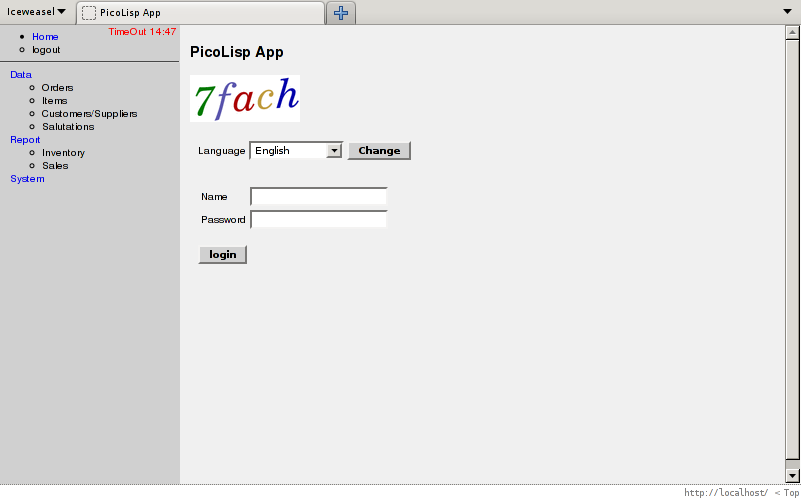
\includegraphics[scale=.4]{graphics/gui-script1.jpg}
\end{figure}


log in on the first page (by typing user name and password, and pressing the
``login'' button),

\begin{figure}[H]
\centering
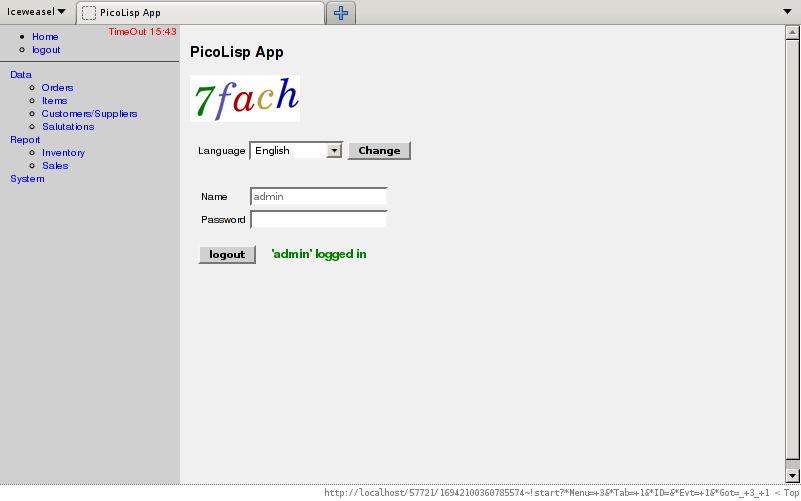
\includegraphics[scale=.4]{graphics/gui-script2.jpg}
\end{figure}


then search for that article in the ``Items'' search dialog (after clicking on the
``Items'' link in the ``Data'' submenu),

\begin{figure}[H]
\centering
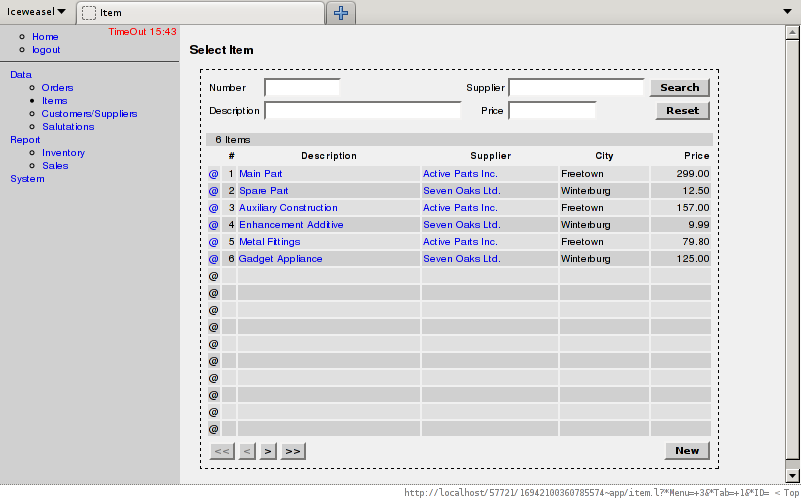
\includegraphics[scale=.4]{graphics/gui-script3.jpg}
\end{figure}


and read the price on the page of that item (here: 12.50).

\begin{figure}[H]
\centering
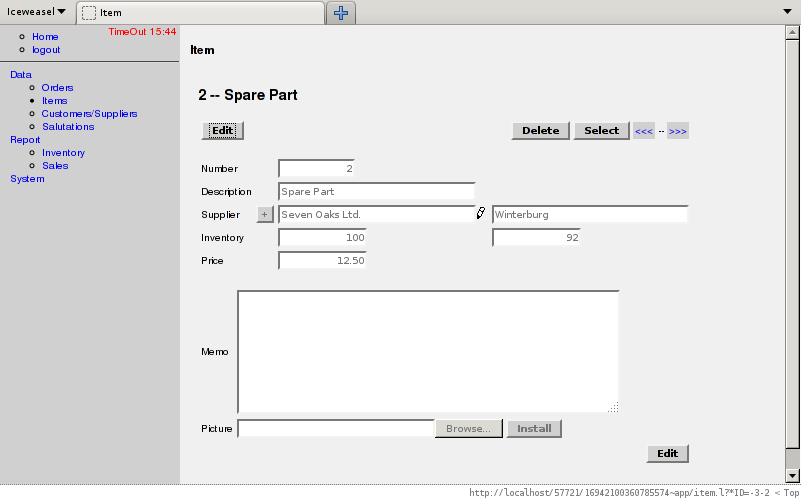
\includegraphics[scale=.4]{graphics/gui-script4.jpg}
\end{figure}


\subsection{Using GUI Scripting}
\label{sec:gui-script-using-gui-scripting}

The same result can be obtained without a browser, by interacting on
the REPL with the remote application. We assume that the demo
application is still running locally at
\underline{http://localhost:8080}\footnote{http://localhost:8080}.

Start PicoLisp, and load the necessary libraries:
\begin{wideverbatim}
   $ pil +
   : (load "@lib/http.l" "@lib/scrape.l")
\end{wideverbatim}

Call \texttt{scrape} to connect to the server
\begin{wideverbatim}
   : (scrape "localhost" 8080)
   -> "PicoLisp App"
\end{wideverbatim}

If you must use the online demo server, call \texttt{(scrape
  "7fach.de" 80 "8080")} instead, telling \texttt{scrape} to connect
to port 80 of that server (where 'httpGate' is running), and then to
dispatch to 8080 (the application's address).

Now log in:
\begin{wideverbatim}
   : (expect "'admin' logged in"
      (enter 3 "admin")
      (enter 4 "admin")
      (press "login") )
   -> NIL
\end{wideverbatim}

(\textbf{Caveat}: Keep in mind a fundamental feature of the PicoLisp
server: Whenever a second log in of the same user from the same IP
address is detected, the first session of that user is automatically
terminated. This means that you cannot run a GUI and a \texttt{scrape}
session with user ``admin'' at the same time. If you already had a gui
session open, it will be \textit{dead} now.)

\texttt{expect} takes a string argument -- a pattern which is to be
expected on the resulting page after the body (the remaining
arguments) was executed. This body enters two values (the user name
and the password) into the appropriate fields, and presses the
``login'' button.

\texttt{enter} takes a field specification and a value. The first call
with \texttt{3} refers to the ``Name'' field, as this is the third
field on the form (the first field is the ``TimeOut'' indicator, and
the second one is the language selector). The next field, field number
\texttt{4}, is the password field.

Finally, \texttt{press} simulates a press of the corresponding button,
and the message ``'admin' logged in'' appears on the page, satisfying
\texttt{expect}.

Then, just as in the GUI, click on the ``Items'' link to open the
dialog. We forgo the \texttt{expect} here, and assume that the dialog
can't fail:

\begin{wideverbatim}
   : (click "Items")
   -> "Item"
\end{wideverbatim}

We also assume that ``Spare Part'' readily appears in the result list
of the search dialog (it was on the second line). A real script would
interact with the dialog to find the desired item. So we just click on
it:

\begin{wideverbatim}
   : (click "Spare Part")
   -> "Item"
\end{wideverbatim}

Now the page of that article is open. Counting the fields, we find
that the price is in the 8th one. We can read that field's value, and
get the same result as in the GUI session above:

\begin{wideverbatim}
   : (value 8)
   -> "12.50"
\end{wideverbatim}

Note that you can also get an overview of the current page with
\texttt{display}:

\begin{wideverbatim}
: (display)
###############
click "Home" "logout" "Data" "Orders" "Items" "Customers/Suppliers"
"Salutations" "Report" "Inventory" "Sales" "System" "<<<" ">>>" "obj"

press "Edit" "Delete" "Select" "+" "Install" "Edit"

value "TimeOut 12:11" "2" "Spare Part" "Seven Oaks UnLtd." "Winterburg" "100"
"98" "12.50"

-> "Item"
\end{wideverbatim}

This helps you to find the positions of links, buttons and fields.

Finally, we should log out:
\begin{wideverbatim}
   : (click "logout")
   -> "PicoLisp App"
\end{wideverbatim}


\section{The Scrape Library}
\label{sec:gui-script-the-scrape-library}

To use the GUI scripting functionality, you need to load
``@lib/http.l`` and ``@lib/scrape.l``. It implements the following
functions:

\begin{itemize}
\item \texttt{(scrape 'host 'port 'how) -> sym | lst} Sets up an
  environment for further operations on an application, which can be
  \texttt{connect}ed on a server at \texttt{host} and \texttt{port},
  and an optional URL argument \texttt{how}. Returns the title of the
  page if no errors occurred, otherwise a list of error messages.

\item \texttt{(expect 'sym . prg)} Executes a \texttt{prg} body
  (holding calls to the functions explained below), and checks for an
  expected pattern \texttt{sym} in the server output.

\item \texttt{(click 'label ['cnt]) -> sym | lst} Simulates the click
  on a link. The first (or \texttt{cnt}'th) link found on the page
  which has \texttt{label} as a prefix is used. Returns the result of
  \texttt{scrape}.

\item \texttt{(press 'label ['cnt]) -> sym | lst} Simulates the press
  of a button. The first (or \texttt{cnt}'th) button found on the page
  which has \texttt{label} as a prefix is used. Returns the result of
  \texttt{scrape}.

\item \texttt{(value 'field ['cnt]) -> sym} Returns the current value
  of the GUI field. The \texttt{field} argument may be either a
  positive number (to specify the \texttt{cnt}'th field on the page),
  a negative number (to specify the \texttt{-cnt}'th last field on the
  page), or the field's name. If the name is given, then \texttt{cnt}
  may specify the form if more than one form is on the page.

\item \texttt{(enter 'field 'sym ['cnt]) -> sym} Enters a value
  \texttt{sym} into the GUI field. The \texttt{field} argument may be
  either a positive number (to specify the \texttt{cnt}'th field on
  the page), a negative number (to specify the \texttt{-cnt}'th last
  field on the page), or the field's name. If the name is given, then
  \texttt{cnt} may specify the form if more than one form is on the
  page.

\item \texttt{(display) -> sym} Display the state of the current page.
  First a line \texttt{\#\#\#\#\#\#\#\#\#\#\#\#\#\#\#} is printed as a visual
  separator, then all available links and buttons, and the values of
  all GUI fields is printed.

\end{itemize}

All these functions can be used interactively (e.g. during development
and debugging of a script), and in stand-alone programs. In the latter
case, they can be used as building-blocks of higher-level functions,
to interact flexibly with forms, dialogs and alerts.

Let your imagination fly!


\title{Manual Page}
\author{Alexander Burger}
% Use \authorrunning{Short Title} for an abbreviated version of
% your contribution title if the original one is too long
\institute{\texttt{abu@software-lab.de}}
%
% Use the package "url.sty" to avoid
% problems with special characters
% used in your e-mail or web address
%


\maketitle

% \section{Manual Page}
% \label{sec:manpage-manual-page}

\begin{abstract}
  This is the PicoLisp Manual Page.
\end{abstract}

\section{NAME}
\label{sec:manpage-name}


pil, picolisp - a fast, lightweight Lisp interpreter

 
\section{SYNOPSIS}
\label{sec:manpage-synopsis}


\textbf{pil} [arguments \ldots{}] [-] [arguments \ldots{}] [+]
 \textbf{/installpath/bin/picolisp} [arguments \ldots{}] [-] [arguments \ldots{}] [+]

 
\section{DESCRIPTION}
\label{sec:manpage-description}

\begin{description}

\item[PicoLisp] is a Lisp interpreter with a small memory footprint, yet
relatively high execution speed. It combines an elegant and powerful
language with built-in database functionality.

\item[pil] is the startup front-end for the interpreter. It takes care of
starting the binary base system and loading a useful runtime
environment.

\item[picolisp] is just the bare interpreter binary. It is usually called in
stand-alone scripts, using the she-bang notation in the first line,
passing the minimal environment in \emph{lib.l} and loading additional files
as needed:

\end{description}

\begin{wideverbatim}
(load ``@ext.l'' ``myfiles/lib.l'' ``myfiles/foo.l'')

(do \ldots{} something \ldots{})

(bye)
\end{wideverbatim}

 
\section{INVOCATION}
\label{sec:manpage-invocation}


\textbf{PicoLisp} has no pre-defined command line flags; applications are free
to define their own. Any built-in or user-level Lisp function can be
invoked from the command line by prefixing it with a hyphen. Examples
for built-in functions useful in this context are \textbf{version} (print the
version number) or \textbf{bye} (exit the interpreter). Therefore, a minimal
call to print the version number and then immediately exit the
interpreter would be:

\begin{wideverbatim}
$ pil -version -bye
\end{wideverbatim}

Any other argument (not starting with a hyphen) should be the name of a
file to be loaded. If the first character of a path or file name is an
at-mark, it will be substituted with the path to the installation
directory.

All arguments are evaluated from left to right, then an interactive
\emph{read-eval-print} loop is entered (with a colon as prompt).

A single hyphen stops the evaluation of the rest of the command line, so
that the remaining arguments may be processed under program control.

If the very last command line argument is a single plus character,
debugging mode is switched on at interpreter startup, before evaluating
any of the command line arguments. A minimal interactive session is
started with:

\begin{wideverbatim}
$ pil +
\end{wideverbatim}


Here you can access the reference manual

\begin{wideverbatim}
 (doc)
\end{wideverbatim}

and the online documentation for most functions,

\begin{wideverbatim}
 (doc 'vi)
\end{wideverbatim}

or directly inspect their sources:

\begin{wideverbatim}
 (vi 'doc)
\end{wideverbatim}

The interpreter can be terminated with

\begin{wideverbatim}
 (bye)
\end{wideverbatim}

or by typing Ctrl-D.

 
\section{FILES}
\label{sec:manpage-files}


Runtime files are maintained in the \~{}/.pil directory:

\begin{wideverbatim}
~{}/.pil/tmp/<pid>/
\end{wideverbatim}


Process-local temporary directories

\begin{wideverbatim}
~{}/.pil/history
\end{wideverbatim}

The line editor's history file

 
\section{BUGS}
\label{sec:manpage-bugs}


\textbf{PicoLisp} doesn't try to protect you from every possible programming
error (``You asked for it, you got it'').

 
\section{AUTHOR}
\label{sec:manpage-author}


Alexander Burger \href{mailto:abu@software-lab.de}{abu@software-lab.de}

 
\section{RESOURCES}
\label{sec:manpage-resources}


\textbf{Home page:}
\href{http://home.picolisp.com}{http://home.picolisp.com}

\textbf{Download:}
\href{http://www.software-lab.de/down.html}{http://www.software-lab.de/down.html}

\title{README}
\author{Alexander Burger}
% Use \authorrunning{Short Title} for an abbreviated version of
% your contribution title if the original one is too long
\institute{\texttt{abu@software-lab.de}}
%
% Use the package "url.sty" to avoid
% problems with special characters
% used in your e-mail or web address
%


\maketitle

% \section{README}
% \label{sec:readme-readme}


\begin{abstract}
  This is the README file of the PicoLisp distribution. 
\end{abstract}

\section{The PicoLisp System}
\label{sec:readme-the-picolisp-system}


\begin{wideverbatim}
  _PI_co Lisp is not _CO_mmon Lisp
\end{wideverbatim}

PicoLisp can be viewed from two different aspects: As a general purpose
programming language, and a dedicated application server framework.


\subsection{Programming Language}
\label{sec:readme-programming-language}

As a programming language, PicoLisp provides a 1-to-1 mapping of a
clean and powerful Lisp derivate, to a simple and efficient virtual
machine. It supports persistent objects as a first class data type,
resulting in a database system of Entity/Relation classes and a
Prolog-like query language tightly integrated into the system.

The virtual machine was designed to be
\begin{description}
\item[Simple] The internal data structure should be as simple as
  possible. Only one single data structure is used to build all higher
  level constructs.
\item[Unlimited] There are no limits imposed upon the language due to
  limitations of the virtual machine architecture. That is, there is
  no upper bound in symbol name length, number digit counts, or data
  structure and buffer sizes, except for the total memory size of the
  host machine.
\item[Dynamic] Behavior should be as dynamic as possible ("run"-time
  vs. "compile"-time). All decisions are delayed till runtime where
  possible. This involves matters like memory management, dynamic
  symbol binding, and late method binding.
\item[Practical] PicoLisp is not just a toy of theoretical value.
  PicoLisp is used since 1988 in actual application development,
  research and production.
\end{description}
   
The language inherits the major advantages of classical Lisp systems like
\begin{itemize}
\item Dynamic data types and structures
\item Formal equivalence of code and data
\item Functional programming style
\item An interactive environment
\end{itemize}

PicoLisp is very different from any other Lisp dialect. This is partly
due to the above design principles, and partly due to its long
development history since 1984.

You can download the latest release version at
http://software-lab.de/down.html

\subsection{Application Server Framework}
\label{sec:readme-application-server-framework}

As an application server framework, PicoLisp provides for

\paragraph{NoSQL Database Management}
\label{par:readme-nosql-database-management}

  \begin{itemize}
    \item Index trees
    \item Object local indexes
    \item Entity/Relation classes
    \item Pilog (PicoLisp Prolog) queries
    \item Multi-user synchronization
    \item DB Garbage collection
    \item Journaling, Replication
  \end{itemize}

\paragraph{User Interface}
\label{par:readme-user-interface}

  \begin{itemize}
    \item Browser GUI
     \item X)HTML/CSS
     \item XMLHttpRequest/JavaScript
  \end{itemize}

\paragraph{Application Server} 
\label{par:readme-application-server}

  \begin{itemize}
    \item Process management
    \item Process family communication
    \item XML I/O
    \item Import/export
    \item User administration
    \item Internationalization
    \item Security
    \item Object linkage
    \item Postscript/Printing
  \end{itemize}


PicoLisp is not an IDE. All program development in Software Lab. is
done using the console, bash, vim and the Lisp interpreter.

The only type of GUI supported for applications is through a browser
via HTML. This makes the client side completely platform independent.
The GUI is created dynamically. Though it uses JavaScript and
XMLHttpRequest for speed improvements, it is fully functional also
without JavaScript or CSS.

The GUI is deeply integrated with - and generated dynamically from -
the application's data model. Because the application logic runs on
the server, multiple users can view and modify the same database
object without conflicts, everyone seeing changes done by other users
on her screen immediately due to the internal process and database
synchronization.

PicoLisp is free software, and you are welcome to use and redistribute
it under the conditions of the MIT/X11 License (see "COPYING").

It compiles and runs on current 32-bit GNU/Linux, FreeBSD, Mac OS X
(Darwin), Cygwin/Win32 (and possibly other) systems. A native 64-bit
version is available for x86-64/Linux, x86-64/SunOS and ppc64/Linux.


% Local variables:
% mode: latex
% TeX-master: "../../editor.tex"
% End:

\title{INSTALL}
\author{Alexander Burger}
% Use \authorrunning{Short Title} for an abbreviated version of
% your contribution title if the original one is too long
\institute{\texttt{abu@software-lab.de}}
%
% Use the package "url.sty" to avoid
% problems with special characters
% used in your e-mail or web address
%


\maketitle

% \section{INSTALL}
% \label{sec:install-install}


\begin{abstract}
This is the INSTALL file from the PicoLisp distribution.   
\end{abstract}


\section{PicoLisp Installation}
\label{sec:install-picolisp-installation}

There is no 'configure' procedure, but the PicoLisp file structure is
simple enough to get along without it (we hope). It should compile and
run on GNU/Linux, FreeBSD, Mac OS X (Darwin), Cygwin/Win32, and
possibly other systems without problems.

PicoLisp supports two installation strategies: Local and Global.

The default (if you just download, unpack and compile the release) is a local
installation. It will not interfere in any way with the world outside its
directory. There is no need to touch any system locations, and you don't have to
be root to install it. Many different versions - or local modifications - of
PicoLisp can co-exist on a single machine.

For a global installation, allowing system-wide access to the executable and
library/documentation files, you can either install it from a ready-made
distribution, or set some symbolic links to one of the local installation
directories as described below.

Note that you are still free to have local installations along with a global
installation, and invoke them explicitly as desired.


\section{Local Installation}
\label{sec:install-local-installation}

\subsection{Unpack the distribution}
\label{sec:install-unpack-the-distribution}

\begin{wideverbatim}
  $ tar xfz picoLisp-XXX.tgz
\end{wideverbatim}

\subsection{Change the directory}
\label{sec:install-change-the-directory}

\begin{wideverbatim}
  $ cd picoLisp-XXX
\end{wideverbatim}

\subsection{Compile the PicoLisp interpreter}
\label{sec:install-compile-the-picolisp-interpreter}

\begin{wideverbatim}
  $ (cd src; make)
\end{wideverbatim}

Or - if you have an x86-64 system (under Linux or SunOS), or a ppc64
system (under Linux) - build the 64-bit version

\begin{wideverbatim}
  $ (cd src64; make)
\end{wideverbatim}

In both cases the executable bin/picolisp will be created.

To build the 64-bit version the first time (bootstrapping), you have the
following three options:

\begin{enumerate}
\item If a Java runtime system (version 1.6 or higher) is installed, it will
build right out of the box.
\item Otherwise, download one of the pre-generated "*.s" file packages
  \begin{itemize}
  \item http://software-lab.de/x86-64.linux.tgz
  \item http://software-lab.de/x86-64.sunOs.tgz
  \item http://software-lab.de/ppc64.linux.tgz
  \end{itemize}
\item Else, build a 32-bit version first, and use the resulting
  bin/picolisp to generate the "*.s" files:
\begin{wideverbatim}
$ (cd src; make)
$ (cd src64; make x86-64.linux)
\end{wideverbatim}
After that, the 64-bit binary can be used to rebuild itself.

Note that on the BSD family of operating systems, 'gmake' must be used
instead of 'make'.
\end{enumerate}


\section{Global Installation}
\label{sec:install-global-installation}

The recommended way for a global installation is to use a picolisp
package from the OS distribution.

If that is not available, you can (as root) create four symbolic links
from /usr/lib, /usr/share and /usr/bin to a local installation
directory

\begin{wideverbatim}
   # ln -s /<installdir> /usr/lib/picolisp
   # ln -s /<installdir> /usr/share/picolisp
   # ln -s /usr/lib/picolisp/bin/picolisp /usr/bin/picolisp
   # ln -s /usr/lib/picolisp/bin/pil /usr/bin/pil
\end{wideverbatim}


\section{Invocation}
\label{sec:install-invocation}

In a global installation, the 'pil' command should be used. You can
either start in plain or in debug mode. The difference is that for
debug mode the command is followed by single plus ('+') sign. The '+'
must be the very last argument on the command line.

\begin{wideverbatim}
   $ pil       # Plain mode
   :

   $ pil +     # Debug mode
   :
\end{wideverbatim}

In both cases, the colon ':' is PicoLisp's prompt. You may enter some
Lisp expression,

\begin{wideverbatim}
 : (+ 1 2 3)
   -> 6
\end{wideverbatim}

To exit the interpreter, enter

\begin{wideverbatim}
 : (bye)
\end{wideverbatim}

or just type Ctrl-D.

For a local invocation, specify a path name, e.g.

\begin{wideverbatim}
   $ ./pil     # Plain mode
   :

   $ ./pil +   # Debug mode
   :
\end{wideverbatim}

or
\begin{wideverbatim}
$ /home/app/pil  # Invoking a local installation from some other directory
\end{wideverbatim}

A shortcut for debug mode is the 'dbg' script:

\begin{wideverbatim}
   $ ./dbg
   :
\end{wideverbatim}

It is available only for local installaions, and is eqivalent to
\begin{wideverbatim}
  $ ./pil +
\end{wideverbatim}

Note that 'pil' can also serve as a template for your own stand-alone scripts.

If you just want to test the ready-to-run Ersatz PicoLisp (it needs a Java
runtime system), use

\begin{wideverbatim}
   $ ersatz/pil +
   :
\end{wideverbatim}

instead of './dbg' or './pil +'.

\section{Documentation}
\label{sec:install-documentation}

For further information, please look at "doc/index.html". There you find the
PicoLisp Reference Manual ("doc/ref.html"), the PicoLisp tutorials
("doc/tut.html", "doc/app.html", "doc/select.html" and "doc/native.html"), and
the frequently asked questions ("doc/faq.html").

For details about the 64-bit version, refer to "doc64/README", "doc64/asm" and
"doc64/structures".

As always, the most accurate and complete documentation is the source code ;-)
Included in the distribution are many utilities and pet projects, including
tests, demo databases and servers, games (chess, minesweeper), 3D animation
(flight simulator), and more.

Any feedback is welcome!
Hope you enjoy :-)



%%%%%%%%%%%%%%%%%%%%%%%%%%%%%%%%%%%%%%%%%%%%%%%%%%%%%%%%%%%%%%%
% sample part title
%
% Copy it to a new file with a new name and use it
% use it as a template for your own input.
%
%%%%%%%%%%%%%%%%%%%%%%%% Springer-Verlag %%%%%%%%%%%%%%%%%%%%%%%%%%


\part{PicoLisp Tutorials}
\title{A PicoLisp Tutorial}
\author{Alexander Burger}
% Use \authorrunning{Short Title} for an abbreviated version of
% your contribution title if the original one is too long
\institute{\texttt{abu@software-lab.de}}
%
% Use the package "url.sty" to avoid
% problems with special characters
% used in your e-mail or web address
%


\maketitle


\begin{abstract}
  This article demonstrates some aspects of the PicoLisp system in
  detail and example. For a general description of the PicoLisp kernel
  please look at the \emph{PicoLisp Reference}.

  This is not a Lisp tutorial, as it assumes some basic knowledge of
  programming, Lisp, and even PicoLisp. Please read these sections in
  the \emph{PicoLisp Reference} before coming back here:
  \emph{Introduction} and \emph{The PicoLisp Machine}. This tutorial
  concentrates on the specificities of PicoLisp, and its differences
  with other Lisp dialects.
\end{abstract}

\section{Now let's start}
\label{sec:tut-now-lets-start}

If not stated otherwise, all examples assume that PicoLisp was started
from a global installation (see \href{ref.html\#inst}{Installation})
from the shell prompt as

\begin{verbatim}
$ pil +
:
\end{verbatim}

It loads the PicoLisp base system and the debugging environment, and
waits for you to enter input lines at the interpreter prompt
(\texttt{:}). You can terminate the interpreter and return to the shell
at any time, by either hitting the \texttt{Ctrl-D} key, or by executing
the function \texttt{(bye)}.

Please note that special handling is done during character input. This
one is incompatible with \texttt{rlwrap} for example but is more
powerful.

\begin{itemize}
\item
  \texttt{vi}-like command-line editing (typos fixes and history with
  ESC, \texttt{h}, \texttt{j}, \texttt{k} and \texttt{l} but not
  arrows),
\item
  auto-formating (underlined) of double-quoted strings (don't try and
  struggle to make \texttt{"} appear).
\end{itemize}

If you prefer to use Emacs, please use the picolisp-mode bundled in
``@lib/el''.

If you feel that you absolutely have to use an IDE, \texttt{rlwrap} or
another input front-end, please remove the entry ``@lib/led.l'' from
``lib.l'' and ``dbg.l''. Note that in this case, however, you will not
have the TAB symbol completion feature available during command line
editing.

\section{Command Line Editing}
\label{sec:tut-command-line-editing}

PicoLisp permanently reads input from the current input channel (i.e.
the console in interactive mode), evaluates it, and prints the result to
the current output channel. This is called a ``read-eval-print-loop''
(REPL).

\subsection{VI-like editing}
\label{sec:tut-vi-like-editing}


It is very helpful - though not absolutely necessary - when you know how
to use the \texttt{vi} editor.

To alleviate the task of manual line input, a command line editor is
provided which is similar to (though much simpler than) the \texttt{readline}
feature of the \texttt{bash} shell. Only a subset of the \texttt{vi} mode is
supported, which is restricted to single-key commands (the ``real'' \texttt{vi}
supports multi-key commands and the modification of most commands with
count prefixes). It is loaded at startup in debug mode, you find its
source in ``lib/led.l''.

You can enter lines in the normal way, correcting mistypes with the
BACKSPACE key, and terminating them with the ENTER key. This is the
\emph{Insert Mode}.

If you hit ESC, you get into \emph{Command Mode}. Now you can navigate
horizontally in the current input line, or vertically in the history of
previously entered lines, with key commands borrowed from the \texttt{vi}
editor (only \texttt{h}, \texttt{j}, \texttt{k} and \texttt{l} and not arrows). Note, however, that
there is always only a single line visible.

Let's say you did some calculation


\begin{wideverbatim}
: (* (+ 2 3) (- 7 2))
-> 25
:
\end{wideverbatim}

If you want to repeat a modified version of this command, using \texttt{8}
instead of \texttt{7}, you don't have to re-type the whole command, but type

\begin{itemize}
\item ESC to get into \emph{Command Mode}
\item \texttt{k} to get one line ``up''
\item \texttt{f} and \texttt{7} to ``find'' the character \texttt{7}
\item \texttt{r} and \texttt{8} to ``replace'' with \texttt{8}
\end{itemize}

Then you hit ENTER to execute the modified line. Instead of jumping to
the \texttt{7} with the ``find'' command, you may also type \texttt{l} (move ``right'')
repeatedly till you reach the correct position.

The key commands in the \emph{Command Mode} are listed below. Some commands
change the mode back to \emph{Insert Mode} as indicated in parentheses.
Deleting or changing a ``word'' take either the current atom (number or
symbol), or a whole expression when the cursor is at a left parenthesis.

\begin{itemize}
\item \texttt{k} - Go up one line
\item \texttt{j} - Go down one line
\item \texttt{l} - Go right one character
\item \texttt{h} - Go left one character
\item \texttt{w} - Go right one word
\item \texttt{b} - Go back (left) one word
\item \texttt{0} - Go to the beginning of the line
\item \texttt{\$} - Go to the end of the line
\item \texttt{i} - Enter \emph{Insert Mode} at the cursor position
\item \texttt{a} - Append (\emph{Insert Mode}) after the cursor position
\item \texttt{A} - Append (\emph{Insert Mode}) at the end of the line
\item \texttt{I} - Insert (\emph{Insert Mode}) at the beginning of the line
\item \texttt{x} - Delete the character at the cursor position
\item \texttt{X} - Delete the character left of the cursor position
\item \texttt{r} - Replace the character at the cursor position with the next key
\item \texttt{s} - Substitute the character at the cursor position (\emph{Insert Mode})
\item \texttt{S} - Substitute the whole line (\emph{Insert Mode})
\item \texttt{d} - Delete the word at the cursor position (\emph{Insert Mode})
\item \texttt{D} - Delete the rest of the line
\item \texttt{c} - Change the word at the cursor position (\emph{Insert Mode})
\item \texttt{C} - Change the rest of the line (\emph{Insert Mode})
\item \texttt{f} - Find next key in the rest of the current line
\item \texttt{p} - Paste data deleted with \texttt{x}, \texttt{X}, \texttt{d} or \texttt{D} after the cursor
   position
\item \texttt{P} - Paste data deleted with \texttt{x}, \texttt{X}, \texttt{d} or \texttt{D} before the cursor
   position
\item \texttt{/} - Accept an input pattern and search the history for it
\item \texttt{n} - Search for next occurrence of pattern (as entered with \texttt{/})
\item \texttt{N} - Search for previous occurrence of pattern
\item \texttt{\%} - Go to matching parenthesis
\item \texttt{\textasciitilde{}} - Convert character to opposite (lower or upper) case and move
   right
\item \texttt{u} - Undo the last change (one level only)
\item \texttt{U} - Undo all changes of the current line
\item \texttt{g} - Display current contents of cut buffer (not in \texttt{vi})
\end{itemize}

Notes:

\begin{itemize}
\item The \texttt{d} command corresponds to the \texttt{dw} command of the \texttt{vi} editor,
   and \texttt{c} corresponds to \texttt{cw}.
\item Search patterns may contain ` \texttt{@} ' characters as wildcards.
\item Lines shorter than 3 characters, lines beginning with a space
   character, or duplicate lines are not entered into the history.
\item The history is stored in the file ``.pil/history'' in the user's home
   directory. The length of the history is limited to 1000 lines.
\end{itemize}

The following two key-combinations work both in Insert and Command Mode:

\begin{itemize}
\item \texttt{Ctrl-D} will immediately terminate the current process.
\item \texttt{Ctrl-X} discards all input, abandons further processing, and returns
   to the interpreter's top level (equivalent to invoking \texttt{quit}). This
   is also useful when the program stopped at a breakpoint (see
   single-stepping \emph{Debugging}), or after program execution was
   interrupted with \texttt{Ctrl-C}.
\end{itemize}

Besides these two keys, in \emph{Insert Mode} only the following keys have a
special meaning:

\begin{itemize}
\item BACKSPACE (\texttt{Ctrl-H}) and DEL erase the character to the left
\item \texttt{Ctrl-V} inserts the next key literally
\item TAB performs symbol and/or path completion: When a symbol (or path)
   name is entered partially and TAB is pressed subsequently, all
   internal symbols (and/or path names in the file system) matching the
   partial input are shown in sequence.
\item ESC terminates \emph{Input Mode} and enters \emph{Command Mode}
\end{itemize}

 
\subsection{Conclusion}
\label{sec:tut-conclusion}


Please take some time to experiment and to get used to command line
editing. It will make life much easier in the future :-)


 
\section{Browsing}
\label{sec:tut-browsing}


PicoLisp provides some functionality for inspecting pieces of data and
code within the running system.

 
\subsection{Basic tools}
\label{sec:tut-basic-tools}


The really basic tools are of course available and their name alone is
enough to know: \texttt{print}, \texttt{size} \ldots{}

But you will appreciate some more powerful tools like:

\begin{itemize}
\item \texttt{match}, a predicate which compares S-expressions with bindable
   wildcards when matching,
\end{itemize}

 
\subsection{Inspect a symbol with \emph{show}}
\label{sec:tut-inspect-a-symbol-with-show}


The most commonly used tool is probably the \texttt{show} function. It takes a
symbolic argument, and shows the symbol's name (if any), followed by its
value cell, and then the contents of the property list on the following
lines (assignment of such things to a symbol can be done with \texttt{set},
\texttt{setq}, and \texttt{put}).


\begin{wideverbatim}
: (setq A '(This is the value))  # Set the value cell of 'A'
-> (This is the value)
: (put 'A 'key1 'val1)           # Store property 'key1'
-> val1
: (put 'A 'key2 'val2)           # and 'key2'
-> val2
: (show 'A)                      # Now 'show' the symbol 'A'
A (This is the value)
   key2 val2
   key1 val1
-> A
\end{wideverbatim}

\texttt{show} accepts an arbitrary number of arguments which are processed
according to the rules of \texttt{get}, resulting in a symbol which is showed
then.


\begin{wideverbatim}
: (put 'B 'a 'A)        # Put 'A' under the 'a'-property of 'B'
-> A
: (setq Lst '(A B C))   # Create a list with 'B' as second argument
-> (A B C)
: (show Lst 2 'a)       # Show the property 'a of the 2nd element of 'Lst'
A (This is the value)   # (which is 'A' again)
   key2 val2
   key1 val1
-> A
\end{wideverbatim}

 
\subsection{Inspect and edit with \emph{edit}}
\label{sec:tut-inspect-and-edit-with-edit}


Similar to \texttt{show} is \texttt{edit}. It takes an arbitrary number of symbolic
arguments, writes them to a temporary file in a format similar to
\texttt{show}, and starts the \texttt{vim} editor with that file.


\begin{wideverbatim}
: (edit 'A 'B)
\end{wideverbatim}

The \texttt{vim} window will look like


\begin{wideverbatim}
A (This is the value)
key1 val1
key2 val2

(********)

B NIL
a A  # (This is the value)

(********)
\end{wideverbatim}

Now you can modify values or properties. You should not touch the
parenthesized asterisks, as they serve as delimiters. If you position
the cursor on the first character of a symbol name and type  \texttt{K} 
(``Keyword lookup''), the editor will be restarted with that symbol added
to the editor window.  \texttt{Q}  (for ``Quit'') will bring you back to the
previous view.

\texttt{edit} is also very useful to browse in a database. You can follow the
links between objects with  \texttt{K} , and even - e.g. for low-level repairs
\begin{itemize}
\item modify the data (but only if you are really sure about what you are
\end{itemize}
doing, and don't forget to \texttt{commit} when you are done).

 
\subsection{Built-in pretty print with \emph{pp}}
\label{sec:tut-built-in-pretty-print-with-pp}


The \emph{pretty-print} function \texttt{pp} takes a symbol that has a function
defined (or two symbols that specify message and class for a method
definition), and displays that definition in a formatted and indented
way.


\begin{wideverbatim}
: (pp 'pretty)
(de pretty (X N . @)
   (setq N (abs (space (or N 0))))
   (while (args) (printsp (next)))
   (if (or (atom X) (>= 12 (size X)))
      (print X)
      (while (== 'quote (car X))
         (prin "'")
         (pop 'X) )
      (let Z X
         (prin "(")
         (cond
            ((memq (print (pop 'X)) *PP)
               (cond
                  ((memq (car Z) *PP1)
                     (if (and (pair (car X)) (pair (cdar X)))
                        (when (>= 12 (size (car X)))
                           (space)
                           (print (pop 'X)) )
                        (space)
                        (print (pop 'X))
                        (when
                           (or
                              (atom (car X))
                              (>= 12 (size (car X))) )
                           (space)
                           (print (pop 'X)) ) ) )
                  ((memq (car Z) *PP2)
                     (inc 'N 3)
                     (loop
                        (prinl)
                        (pretty (cadr X) N (car X))
                        (NIL (setq X (cddr X)) (space)) ) )

\end{wideverbatim}

\begin{wideverbatim}


                  ((or (atom (car X)) (>= 12 (size (car X))))
                     (space)
                     (print (pop 'X)) ) ) )
            ((and (memq (car Z) *PP3) (>= 12 (size (head 2 X))))
               (space)
               (print (pop 'X) (pop 'X)) ) )
         (when X
            (loop
               (T (== Z X) (prin " ."))
               (T (atom X) (prin " . ") (print X))
               (prinl)
               (pretty (pop 'X) (+ 3 N))
               (NIL X) )
            (space) )
         (prin ")") ) ) )
-> pretty
\end{wideverbatim}

The style is the same as we use in source files:

\begin{itemize}
\item The indentation level is three spaces
\item If a list is too long (to be precise: if its \texttt{size} is greater than
   12), pretty-print the CAR on the current line, and each element of
   the CDR recursively on its own line.
\item A closing parenthesis a preceded by a space if the corresponding open
   parenthesis is not on the same line
\end{itemize}

 
\subsection{Inspect elements one by one with \emph{more}}
\label{sec:tut-inspect-elements-one-by-one-with-more}


\texttt{more} is a simple tool that displays the elements of a list one by one.
It stops after each element and waits for input. If you just hit ENTER,
\texttt{more} continues with the next element, otherwise (usually I type a dot
(\texttt{.}) followed by ENTER) it terminates.


\begin{wideverbatim}
: (more (1 2 3 4 5 6))
1                          # Hit ENTER
2.                         # Hit '.' and ENTER
-> T                       # stopped
\end{wideverbatim}

Optionally \texttt{more} takes a function as a second argument and applies that
function to each element (instead of the default \texttt{print}). Here, often
\texttt{show} or \texttt{pp} (see below) is used.


\begin{wideverbatim}
: (more '(A B))            # Step through 'A' and 'B'
A
B
-> NIL
: (more '(A B) show)       # Step through 'A' and 'B' with 'show'
A (This is the value)      # showing 'A'
   key2 val2
   key1 val1
                           # Hit ENTER
B NIL                      # showing 'B'
   a A
-> NIL
\end{wideverbatim}

 
\subsection{Search through available symbols with \emph{what}}
\label{sec:tut-search-through-available-symbols-with-what}


The \texttt{what} function returns a list of all internal symbols in the system
which match a given pattern (with  \texttt{@}  wildcard characters).


\begin{wideverbatim}
: (what "prin@")
-> (prin print prinl print> printsp println)
\end{wideverbatim}

 
\subsection{Search through values or properties of symbols with \emph{who}}
\label{sec:tut-search-through-values-or-properties-of-symbols-with-can}


The function \texttt{can} returns a list which indicates which classes \emph{can}
accept a given message. Again, this list is suitable for iteration with
\texttt{pp}:


\begin{wideverbatim}
: (can 'del>)                                   # Which classes accept 'del>' ?
-> ((del> . +List) (del> . +Entity) (del> . +relation))

: (more (can 'del>) pp)                         # Inspect the methods with 'pp'
(dm (del> . +List) (Obj Old Val)
   (and ((<> Old Val) (delete Val Old)) )

(dm (del> . +Entity) (Var Val)
   (when
      (and
         Val
         (has> (meta This Var) Val (get This Var)) )

\end{wideverbatim}

\begin{wideverbatim}


      (let Old (get This Var)
         (rel>
            (meta This Var)
            This
            Old
            (put This Var (del> (meta This Var) This Old @)) )
         (when (asoq Var (meta This 'Aux))
            (relAux This Var Old (cdr @)) )
         (upd> This Var Old) ) ) )

(dm (del> . +relation) (Obj Old Val)
   (and ((<> Old Val) Val) )
\end{wideverbatim}

 
\subsection{Inspect dependencies with \emph{dep}}
\label{sec:tut-inspect-dependencies-with-dep}


\texttt{dep} shows the dependencies in a class hierarchy. That is, for a given
class it displays the tree of its (super)class(es) above it, and the
tree of its subclasses below it.

To view the complete hierarchy of input fields, we start with the root
class \texttt{+relation}:


\begin{wideverbatim}
: (dep '+relation)
+relation
   +Bag
   +Any
   +Blob
   +Link
      +Joint
   +Bool
   +Symbol
      +String
   +Number
      +Time
      +Date
-> +relation
\end{wideverbatim}

If we are interested in \texttt{+Link}:


\begin{wideverbatim}
: (dep '+Link)
   +relation
+Link
   +Joint
-> +Link
\end{wideverbatim}

This says that \texttt{+Link} is a subclass of \texttt{+relation}, and has a single
subclass (\texttt{+Joint}).


 
\section{Defining Functions}
\label{sec:tut-defining-functions}


Most of the time during programming is spent defining functions (or
methods). In the following we will concentrate on functions, but most
will be true for methods as well except for using \texttt{dm} instead of \texttt{de}.

 
\subsection{Functions with no argument}
\label{sec:tut-functions-with-no-argument}


The notorious ``Hello world'' function must be defined:


\begin{wideverbatim}
: (de hello ()
   (prinl "Hello world") )
-> hello
\end{wideverbatim}

The \texttt{()} in the first line indicates a function without arguments. The
body of the function is in the second line, consisting of a single
statement. The last line is the return value of \texttt{de}, which here is the
defined symbol. From now on we will omit the return values of examples
when they are unimportant.

Now you can call this function this way:


\begin{wideverbatim}
: (hello)
Hello world
\end{wideverbatim}

 
\subsection{Functions with one argument}
\label{sec:tut-functions-with-one-argument}


A function with an argument might be defined this way:


\begin{wideverbatim}
: (de hello (X)
   (prinl "Hello " X) )
# hello redefined
-> hello
\end{wideverbatim}

PicoLisp informs you that you have just redefined the function. This
might be a useful warning in case you forgot that a bound symbol with
that name already existed.


\begin{wideverbatim}
: (hello "world")
Hello world
\end{wideverbatim}


\begin{wideverbatim}
: (hello "Alex")
Hello Alex
\end{wideverbatim}

 
\subsection{Preventing arguments evaluation and variable number of arguments}
\label{sec:tut-preventing-arguments-evaluation-and-variable-number-of-arguments}


Normally, PicoLisp evaluates the arguments before it passes them to a
function:


\begin{wideverbatim}
: (hello (+ 1 2 3))
Hello 6
\end{wideverbatim}


\begin{wideverbatim}
: (setq A 1  B 2)       # Set 'A' to 1 and 'B' to 2
-> 2
: (de foo (X Y)         # 'foo' returns the list of its arguments
   (list X Y) )
-> foo
: (foo A B)             # Now call 'foo' with 'A' and 'B'
-> (1 2)                # -> We get a list of 1 and 2, the values of 'A' and 'B'
\end{wideverbatim}

In some cases you don't want that. For some functions (\texttt{setq} for
example) it is better if the function gets all arguments unevaluated,
and can decide for itself what to do with them.

For such cases you do not define the function with a \emph{list} of
parameters, but give it a \emph{single atomic} parameter instead. PicoLisp
will then bind all (unevaluated) arguments as a list to that parameter.


\begin{wideverbatim}
: (de foo X
   (list (car X) (cadr X)) )        # 'foo' lists the first two arguments

: (foo A B)                         # Now call it again
-> (A B)                            # -> We don't get '(1 2)', but '(A B)'

: (de foo X
   (list (car X) (eval (cadr X))) ) # Now evaluate only the second argument

: (foo A B)
-> (A 2)                            # -> We get '(A 2)'
\end{wideverbatim}

 
\subsection{Mixing evaluated arguments and variable number of unevaluated}
\label{sec:tut-mixing-evaluated-arguments-and-variable-number-of-unevaluated}

arguments

As a logical consequence, you can combine these principles. To define a
function with 2 evaluated and an arbitrary number of unevaluated
arguments:


\begin{wideverbatim}
: (de foo (X Y . Z)     # Evaluate only the first two args
   (list X Y Z) )

: (foo A B C D E)
-> (1 2 (C D E))        # -> Get the value of 'A' and 'B' and the remaining list
\end{wideverbatim}

 
\subsection{Variable number of evaluated arguments}
\label{sec:tut-variable-number-of-evaluated-arguments}


More common, in fact, is the case where you want to pass an arbitrary
number of \emph{evaluated} arguments to a function. For that, PicoLisp
recognizes the symbol \texttt{@} as a single atomic parameter and remembers all
evaluated arguments in an internal frame. This frame can then be
accessed sequentially with the \texttt{args}, \texttt{next}, \texttt{arg} and \texttt{rest}
functions.


\begin{wideverbatim}
: (de foo @
   (list (next) (next)) )     # Get the first two arguments

: (foo A B)
-> (1 2)
\end{wideverbatim}

Again, this can be combined:


\begin{wideverbatim}
: (de foo (X Y . @)
   (list X Y (next) (next)) ) # 'X' and 'Y' are fixed arguments

: (foo A B (+ 3 4) (* 3 4))
-> (1 2 7 12)                 # All arguments are evaluated
\end{wideverbatim}

These examples are not very useful, because the advantage of a variable
number of arguments is not used. A function that prints all its
evaluated numeric arguments, each on a line followed by its squared
value:


\begin{wideverbatim}
: (de foo @
   (while (args)                            # Check if there are some args left
      (println (next) (* (arg) (arg))) ) )  # Call the last arg (next) returned

: (foo (+ 2 3) (- 7 1) 1234 (* 9 9))
5 25
6 36
1234 1522756
81 6561
-> 6561
\end{wideverbatim}

This next example shows the behaviour of \texttt{args} and \texttt{rest}:


\begin{wideverbatim}
: (de foo @
   (while (args)
      (next)
      (println (arg) (args) (rest)) ) )
: (foo 1 2 3)
1 T (2 3)
2 T (3)
3 NIL NIL
\end{wideverbatim}

Finally, it is possible to pass all these evaluated arguments to another
function, using \texttt{pass}:


\begin{wideverbatim}
: (de foo @
   (pass println 9 8 7)       # First print all arguments preceded by 9, 8, 7
   (pass + 9 8 7) )           # Then add all these values

: (foo (+ 2 3) (- 7 1) 1234 (* 9 9))
9 8 7 5 6 1234 81             # Printing ...
-> 1350                       # Return the result
\end{wideverbatim}

 
\subsection{Anonymous functions without the \emph{lambda} keyword}
\label{sec:tut-anonymous-functions-without-the-lambda}


There's no distinction between code and data in PicoLisp, \texttt{quote} will
do what you want (see also \emph{this FAQ entry}).


\begin{wideverbatim}
: ((quote (X) (* X X)) 9)
-> 81
\end{wideverbatim}


\begin{wideverbatim}
: (setq f '((X) (* X X)))  # This is equivalent to (de f (X) (* X X))
-> ((X) (* X X))
: f
-> ((X) (* X X))
: (f 3)
-> 9
\end{wideverbatim}

 
\section{Debugging}
\label{sec:tut-debugging}


There are two major ways to debug functions (and methods) at runtime:
\emph{Tracing} and \emph{single-stepping}.

In this section we will use the REPL to explore the debugging
facilities, but in the \emph{Scripting} section, you will learn
how to launch PicoLisp scripts with some selected functions debugged:


\begin{wideverbatim}
$ pil app/file1.l -"trace 'foo" -main -"debug 'bar" app/file2.l +
\end{wideverbatim}

 
\subsection{Tracing}
\label{sec:tut-tracing}


\emph{Tracing} means letting functions of interest print their name and
arguments when they are entered, and their name again and the return
value when they are exited.

For demonstration, let's define the unavoidable factorial function (or
just \texttt{load} the file ``\texttt{@doc/fun.l}''):


\begin{wideverbatim}
(de fact (N)
   (if (=0 N)
      1
      (* N (fact (dec N))) ) )
\end{wideverbatim}

With \texttt{trace} we can put it in trace mode:


\begin{wideverbatim}
: (trace 'fact)
-> fact
\end{wideverbatim}

Calling \texttt{fact} now will display its execution trace.


\begin{wideverbatim}
: (fact 3)
 fact : 3
  fact : 2
   fact : 1
    fact : 0
    fact = 1
   fact = 1
  fact = 2
 fact = 6
-> 6
\end{wideverbatim}

As can be seen here, each level of function call will indent by an
additional space. Upon function entry, the name is separated from the
arguments with a colon (\texttt{:}), and upon function exit with an equals sign
 \texttt{=}  from the return value.

\texttt{trace} works by modifying the function body, so generally it works only
for functions defined as lists (lambda expressions, see
\emph{Evaluation}). Tracing a C-function is possible, however,
when it is a function that evaluates all its arguments.

So let's trace the functions \texttt{=0} and \texttt{*}:


\begin{wideverbatim}
: (trace '=0)
-> =0
: (trace '*)
-> *
\end{wideverbatim}

If we call \texttt{fact} again, we see the additional output:


\begin{wideverbatim}
: (fact 3)
 fact : 3
  =0 : 3
  =0 = NIL
  fact : 2
   =0 : 2
   =0 = NIL
   fact : 1
    =0 : 1
    =0 = NIL
    fact : 0
     =0 : 0
     =0 = 0
    fact = 1
    * : 1 1
    * = 1
   fact = 1
   * : 2 1
   * = 2
  fact = 2
  * : 3 2
  * = 6
 fact = 6
-> 6
\end{wideverbatim}

To reset a function to its untraced state, call \texttt{untrace}:


\begin{wideverbatim}
: (untrace 'fact)
-> fact
: (untrace '=0)
-> =0
: (untrace '*)
-> *
\end{wideverbatim}

or simply use \texttt{mapc}:

\begin{wideverbatim}
: (mapc untrace '(fact =0 *))
-> *
\end{wideverbatim}

 
\subsection{Single-stepping}
\label{sec:tut-single-stepping}


\emph{Single-stepping} means to execute a function step by step, giving the
programmer an opportunity to look more closely at what is happening. The
function \texttt{debug} inserts a breakpoint into each top-level expression of
a function. When the function is called, it stops at each breakpoint,
displays the expression it is about to execute next (this expression is
also stored into the global variable \texttt{\textasciicircum{}}) and enters a read-eval-loop.
The programmer can then

\begin{itemize}
\item inspect the current environment by typing variable names or calling
   functions
\item execute \texttt{(d)} to recursively debug the next expression (looping
   through subexpressions of this expression)
\item execute \texttt{(e)} to evaluate the next expression, to see what will
   happen without actually advancing on
\item type ENTER (that is, enter an empty line) to leave the read-eval loop
   and continue with the next expression
\end{itemize}

Thus, in the simplest case, single-stepping consists of just hitting
ENTER repeatedly to step through the function.

To try it out, let's look at the \texttt{stamp} system function. You may need
to have a look at

\begin{itemize}
\item \texttt{=T} (T test),
\item \texttt{date} and \texttt{time} (grab system date and time)
\item \texttt{default} (conditional assignments)
\item \texttt{pack} (kind of concatenation), and
\item \texttt{dat\$} and \texttt{tim\$} (date and time formats)
\end{itemize}

to understand this definition.


\begin{wideverbatim}
: (pp 'stamp)
(de stamp (Dat Tim)
   (and (=T Dat) (setq Dat (date T)))
   (default Dat (date) Tim (time T))
   (pack (dat$ Dat "-") " " (tim$ Tim T)) )
-> stamp
\end{wideverbatim}


\begin{wideverbatim}
: (debug 'stamp)                       # Debug it
-> T
: (stamp)                              # Call it again
(and (=T Dat) (setq Dat (date T)))     # stopped at first expression
!                                      # ENTER
(default Dat (date) Tim (time T))      # second expression
!                                      # ENTER
(pack (dat$ Dat "-") " " (tim$ ...     # third expression
! Tim                                  # inspect 'Tim' variable
-> 41908
! (time Tim)                           # convert it
-> (11 38 28)
!                                      # ENTER
-> "2004-10-29 11:38:28"               # done, as there are only 3 expressions
\end{wideverbatim}

Now we execute it again, but this time we want to look at what's
happening inside the second expression.


\begin{wideverbatim}
: (stamp)                              # Call it again
(and (=T Dat) (setq Dat (date T)))
!                                      # ENTER
(default Dat (date) Tim (time T))
!                                      # ENTER
(pack (dat$ Dat "-") " " (tim$ ...     # here we want to look closer
! (d)                                  # debug this expression
-> T
!                                      # ENTER
(dat$ Dat "-")                         # stopped at first subexpression
! (e)                                  # evaluate it
-> "2004-10-29"
!                                      # ENTER
(tim$ Tim T)                           # stopped at second subexpression
! (e)                                  # evaluate it
-> "11:40:44"
!                                      # ENTER
-> "2004-10-29 11:40:44"               # done
\end{wideverbatim}

The breakpoints still remain in the function body. We can see them when
we pretty-print it:


\begin{wideverbatim}
: (pp 'stamp)
(de stamp (Dat Tim)
   (! and (=T Dat) (setq Dat (date T)))
   (! default Dat (date) Tim (time T))
   (! pack
      (! dat$ Dat "-")
      " "
      (! tim$ Tim T) ) )
-> stamp
\end{wideverbatim}

To reset the function to its normal state, call \texttt{unbug}:


\begin{wideverbatim}
: (unbug 'stamp)
\end{wideverbatim}

Often, you will not want to single-step a whole function. Just use
\texttt{edit} (see above) to insert a single breakpoint (the exclamation mark
followed by a space) as CAR of an expression, and run your program.
Execution will then stop there as described above; you can inspect the
environment and continue execution with ENTER when you are done.

 
\section{Functional I/O}
\label{sec:tut-functional-i/o}


Input and output in PicoLisp is functional, in the sense that there are
not variables assigned to file descriptors, which need then to be passed
to I/O functions for reading, writing and closing. Instead, these
functions operate on implicit input and output channels, which are
created and maintained as dynamic environments.

Standard input and standard output are the default channels. Try reading
a single expression:


\begin{wideverbatim}
: (read)
(a b c)        # Console input
-> (a b c)
\end{wideverbatim}

To read from a file, we redirect the input with \texttt{in}. Note that comments
and whitespace are automatically skipped by \texttt{read}:


\begin{wideverbatim}
: (in "@doc/fun.l" (read))
-> (de fact (N) (if (=0 N) 1 (* N (fact (dec N)))))
\end{wideverbatim}

The \texttt{skip} function can also be used directly. To get the first
non-white character in the file with \texttt{char}:


\begin{wideverbatim}
: (in "@doc/fun.l" (skip "#") (char))
-> "("
\end{wideverbatim}

\texttt{from} searches through the input stream for given patterns. Typically,
this is not done with Lisp source files (there are better ways), but for
a simple example let's extract all items immediately following \texttt{fact} in
the file,


\begin{wideverbatim}
: (in "@doc/fun.l" (while (from "fact ") (println (read))))
(N)
(dec N)
\end{wideverbatim}

or the word following ``(de'' with \texttt{till}:


\begin{wideverbatim}
: (in "@doc/fun.l" (from "(de ") (till " " T)))
-> "fact"
\end{wideverbatim}

With \texttt{line}, a line of characters is read, either into a single
\emph{transient} symbol (the type used by PicoLisp
for strings),


\begin{wideverbatim}
: (in "@doc/tut.html" (line T))
-> "<!DOCTYPE HTML PUBLIC "-//W3C//DTD HTML 4.0 Transitional//EN" "http://..."
\end{wideverbatim}

or into a list of symbols (characters):


\begin{wideverbatim}
: (in "@doc/tut.html" (line))
-> ("<" "!" "D" "O" "C" "T" "Y" "P" "E" " " "H" "T" "M" "L" ...
\end{wideverbatim}

\texttt{line} is typically used to read tabular data from a file. Additional
arguments can split the line into fixed-width fields, as described in
the \texttt{reference manual}. If, however, the data are of variable width,
delimited by some special character, the \texttt{split} function can be used to
extract the fields. A typical way to import the contents of such a file
is:


\begin{wideverbatim}
(load "@lib/import.l")

(in '("bin/utf2" "importFile.txt")              # Pipe: Convert to UTF-8
   (until (eof)                                 # Process whole file
      (let L (split (line) "^I")                # TAB-delimited data
         ... use 'getStr', 'getNum' etc ...     # process them
\end{wideverbatim}

Some more examples with \texttt{echo}:


\begin{wideverbatim}
(in "a"                                         # Copy the first 40 Bytes
   (out "b"                                     # from file "a" to file "b"
      (echo 40) ) )

(in "@doc/tut.html"                             # Show the HTTP-header
   (line)
   (echo "<body>") )

(out "file.mac"                                 # Convert to Macintosh
   (in "file.txt"                               # from Unix or DOS format:
      (while (char)
         (prin
            (case @
               ("^M" NIL)                       # ignore CR
               ("^J" "^M")                      # convert CR to LF
               (T @) ) ) ) ) )                  # otherwise no change

(out "c"                                        # Merge the contents of "a"
   (in "b"                                      # and "b" into "c"
      (in "a"
         (while (read)                          # Read an item from "a",
            (println @ (in -1 (read))) ) ) ) )  # print it with an item from "b"
\end{wideverbatim}

 
\section{Scripting}
\label{sec:tut-scripting}


There are two possibilities to get the PicoLisp interpreter into doing
useful work: via command line arguments, or as a stand-alone script.

 
\subsection{Command line arguments for the PicoLisp interpreter}
\label{sec:tut-command-line-arguments-for-the-picolisp-interpreter}


The command line can specify either files for execution, or arbitrary
Lisp expressions for direct evaluation (see
\emph{Invocation}): if an argument starts with a hyphen, it
is evaluated, otherwise it is \texttt{load} d as a file. A typical invocation
might look like:


\begin{wideverbatim}
$ pil app/file1.l -main app/file2.l +
\end{wideverbatim}

It loads the debugging environment, an application source file, calls
the main function, and then loads another application source. In a
typical development and debugging session, this line is often modified
using the shell's history mechanisms, e.g. by inserting debugging
statements:


\begin{wideverbatim}
$ pil app/file1.l -"trace 'foo" -main -"debug 'bar" app/file2.l +
\end{wideverbatim}

Another convenience during debugging and testing is to put things into
the command line (shell history) which would otherwise have to be done
each time in the application's user interface:


\begin{wideverbatim}
$ pil app/file1.l -main app/file2.l -go -'login "name" "password"' +
\end{wideverbatim}

The final production release of an application usually includes a shell
script, which initializes the environment, does some bookkeeping and
cleanup, and calls the application with a proper command line. It is no
problem if the command line is long and complicated.

For small utility programs, however, this is overkill. Enter full
PicoLisp scripts.

 
\subsection{PicoLisp scripts}
\label{sec:tut-picolisp-scripts}


It is better to write a single executable file using the mechanisms of
``interpreter files''. If the first two characters in an executable file
are ` \texttt{\#!} ', the operating system kernel will pass this file to an
interpreter program whose pathname is given in the first line
(optionally followed by a single argument). This is fast and efficient,
because the overhead of a subshell is avoided.

Let's assume you installed PicoLisp in the directory
``/home/foo/picolisp/'', and put links to the executable and the
installation directory as:


\begin{wideverbatim}
$ ln -s /home/foo/picolisp /usr/lib/picolisp
$ ln -s /usr/lib/picolisp/bin/picolisp /usr/bin/picolisp
\end{wideverbatim}

Then a simple hello-world script might look like:


\begin{wideverbatim}
#!/usr/bin/picolisp /usr/lib/picolisp/lib.l
(prinl "Hello world!")
(bye)
\end{wideverbatim}

If you write this into a text file, and use \texttt{chmod} to set it to
``executable'', it can be executed like any other command. Note that
(because \texttt{\#} is the comment character in PicoLisp) the first line will
not be interpreted, and you can still use that file as a normal command
line argument to PicoLisp (useful during debugging).

 
\subsection{Grab command line arguments from PicoLisp scripts}
\label{sec:tut-grab-command-line-arguments-from-picolisp-scripts}


The fact that a hyphen causes evaluation of command line arguments can
be used to simulate something like command line options. The following
script defines two functions \texttt{a} and \texttt{f}, and then calls \texttt{(load T)} to
process the rest of the command line (which otherwise would be ignored
because of the \texttt{(bye)} statement):


\begin{wideverbatim}
#!/usr/bin/picolisp /usr/lib/picolisp/lib.l

(de a ()
   (println '-a '-> (opt)) )

(de f ()
   (println '-f '-> (opt)) )

(load T)
(bye)
\end{wideverbatim}

(\texttt{opt} retrieves the next command line option)

Calling this script (let's say we named it ``testOpts'') gives:


\begin{wideverbatim}
$ ./testOpts -f abc
-f -> "abc"
$ ./testOpts -a xxx  -f yyy
-a -> "xxx"
-f -> "yyy"
\end{wideverbatim}

We have to be aware of the fact, however, that the aggregation of
arguments like


\begin{wideverbatim}
$ ./testOpts -axxx  -fyyy
\end{wideverbatim}

or


\begin{wideverbatim}
$ ./testOpts -af yyy
\end{wideverbatim}

cannot be achieved with this simple and general mechanism of command
line processing.

 
\subsection{Run scripts from arbitrary places on the host file system}
\label{sec:tut-run-scripts-from-arbitrary-places-on-the-host-file-system}


Utilities are typically used outside the context of the PicoLisp
environment. All examples above assumed that the current working
directory is the PicoLisp installation directory, which is usually all
right for applications developed in that environment. Command line file
arguments like ``app/file1.l'' will be properly found.

To allow utilities to run in arbitrary places on the host file system,
the concept of \emph{home directory substitution} was introduced. The
interpreter remembers internally at start-up the pathname of its first
argument (usually ``lib.l''), and substitutes any leading ` \texttt{@} ' character
in subsequent file names with that pathname. Thus, to run the above
example in some other place, simply write:


\begin{wideverbatim}
$ /home/foo/picolisp/dbg @app/file1.l -main @app/file2.l
\end{wideverbatim}

that is, supply a full path name to the initial command (here `p'), or
put it into your \texttt{PATH} variable, and prefix each file which has to be
loaded from the PicoLisp home directory with a \texttt{@} character. ``Normal''
files (not prefixed by \texttt{@}) will be opened or created relative to the
current working directory as usual.

Stand-alone scripts will often want to load additional modules from the
PicoLisp environment, beyond the ``lib.l'' we provided in the first line
of the hello-world script. Typically, at least a call to


\begin{wideverbatim}
(load "@lib/misc.l")
\end{wideverbatim}

(note the home directory substitution) will be included near the
beginning of the script.

As a more complete example, here is a script which extracts the date,
name and size of the latest official PicoLisp release version from the
download web site, and prints it to standard output:


\begin{wideverbatim}
#!/usr/bin/picolisp /usr/lib/picolisp/lib.l

(load "@lib/misc.l" "@lib/http.l")

(use (@Date @Name @Size)
   (when
      (match
         '(@Date " " "-" " " @Name " " "(" @Size ")")
         (client "software-lab.de" 80 "down.html"
            (from "Release Archive")
            (from ".tgz">")
            (till "") ) )
      (prinl @Name)
      (prinl @Date " -- " @Size) ) )

(bye)
\end{wideverbatim}

 
\subsection{Editing scripts}
\label{sec:tut-editing-scripts}


We recommend that you have a terminal window open, and try the examples
by yourself. You may either type them in, directly to the PicoLisp
interpreter, or edit a separate source file (e.g. \texttt{''@doc/fun.l''}) in a
second terminal window and load it into PicoLisp with


\begin{wideverbatim}
: (load "@doc/fun.l")
\end{wideverbatim}

each time you have modified and saved it.

 
\subsection{Editing scripts with vi}
\label{sec:tut-editing-scripts-with-vi}


Once a function is loaded from a source file, you can call `vim'
directly on that function with


\begin{wideverbatim}
: (vi 'fact)
\end{wideverbatim}

The function `vi' opens the appropriate source file, and jumps to the
right line where `fact' is defined. When you modify it, you can simply
call `ld' to (re)load that source file


\begin{wideverbatim}
: (ld)
\end{wideverbatim}

 
\section{Objects and Classes}
\label{sec:tut-objects-and-classes}


The PicoLisp object model is very simple, yet flexible and powerful.
Objects as well as classes are both implemented as symbols. In fact,
there is no formal difference between objects and classes; classes are
more a conceptual design consideration in the head of the programmer
than a physical reality.

Having said this, we declare that normally:

\begin{enumerate}
\item A Class
\begin{itemize}
\item Has a name (interned symbol)
\item Has method definitions and superclass(es) in the value cell
\item May have class variables (attributes) in the property list
\end{itemize}
\item An Object
\begin{itemize}
\item Has no name (anonymous symbol) or is an external symbol
\item Has class(es) (and optionally method definitions) in the value
      cell
\item Has instance variables (attributes) in the property list
\end{itemize}
\end{enumerate}

So the main difference between classes and objects is that the former
ones usually are internal symbols. By convention, their names start with
a  \texttt{+} . Sometimes it makes sense, however, to create named objects (as
global singletons, for example), or even anonymous classes.

Both classes and objects have a list in their value cell, consisting of
method definitions (often empty for objects) and (super)class(es). And
both classes and objects have local data in their property lists (often
empty for classes). This implies, that any given object (as an instance
of a class) may have private (object-local) methods defined.

It is rather difficult to contrive a simple OOP example. We constructed
a hierarchy of geometric shapes, with a base class \texttt{+Shape} and two
subclasses \texttt{+Rectangle} and \texttt{+Circle}.

The source code is included as ``\texttt{@doc/shape.l}'' in the PicoLisp
distribution, so you don't have to type it in. Just \texttt{load} the file, or
start it from the shell as:


\begin{wideverbatim}
$ pil @doc/shape.l +
\end{wideverbatim}

Let's look at it piece by piece. Here's the base class:


\begin{wideverbatim}
(class +Shape)
# x y

(dm T (X Y)
   (=: x X)
   (=: y Y) )

(dm move> (DX DY)
   (inc (:: x) DX)
   (inc (:: y) DY) )
\end{wideverbatim}

The first line `\texttt{(class +Shape)}' defines the symbol
\texttt{+Shape} as a class without superclasses. The following method
definitions will go to that class.

The comment  \texttt{\# x y}  in the second line is just a convention, to
indicate what instance variables (properties) that class uses. As
PicoLisp is a dynamic language, a class can be extended at runtime with
any number of properties, and there is nothing like a fixed object size
or structure. This comment is a hint of what the programmer thinks to be
essential and typical for that class. In the case of \texttt{+Shape}, \texttt{x} and
\texttt{y} are the coordinates of the shape's origin.

Then we have two method definitions, using the keyword \texttt{dm} for ``define
method''. The first method is special, in that its name is \texttt{T}. Each time
a new object is created, and a method with that name is found in its
class hierarchy, that method will be executed. Though this looks like a
``constructor'' in other programming languages, it should probably better
be called ``initializer''. The \texttt{T} method of \texttt{+Shape} takes two arguments
\texttt{X} and \texttt{Y}, and stores them in the object's property list.

The second method \texttt{move>} changes the object's origin by adding the
offset values \texttt{DX} and \texttt{DY} to the object's origin.

Now to the first derived class:


\begin{wideverbatim}
(class +Rectangle +Shape)
# dx dy

(dm T (X Y DX DY)
   (super X Y)
   (=: dx DX)
   (=: dy DY) )

(dm area> ()
   (* (: dx) (: dy)) )

(dm perimeter> ()
   (* 2 (+ (: dx) (: dy))) )

(dm draw> ()
   (drawRect (: x) (: y) (: dx) (: dy)) )
\end{wideverbatim}

\texttt{+Rectangle} is defined as a subclass of \texttt{+Shape}. The comment
 \texttt{\# dx dy}  indicates that \texttt{+Rectangle} has a width and a height in
addition to the origin coordinates inherited from \texttt{+Shape}.

The \texttt{T} method passes the origin coordinates \texttt{X} and \texttt{Y} to the \texttt{T}
method of the superclass (\texttt{+Shape}), then stores the width and height
parameters into \texttt{dx} and \texttt{dy}.

Next we define the methods \texttt{area>} and \texttt{perimeter>} which do some
obvious calculations, and a method \texttt{draw>} which is supposed to draw the
shape on the screen by calling some hypothetical function \texttt{drawRect}.

Finally, we define a \texttt{+Circle} class in an analog way, postulating the
hypothetical function \texttt{drawCircle}:


\begin{wideverbatim}
(class +Circle +Shape)
# r

(dm T (X Y R)
   (super X Y)
   (=: r R) )

(dm area> ()
   (*/ (: r) (: r) 31415927 10000000) )

(dm perimeter> ()
   (*/ 2 (: r) 31415927 10000000) )

(dm draw> ()
   (drawCircle (: x) (: y) (: r)) )
\end{wideverbatim}

Now we can experiment with geometrical shapes. We create a rectangle at
point (0,0) with a width of 30 and a height of 20, and keep it in the
variable \texttt{R}:


\begin{wideverbatim}
: (setq R (new '(+Rectangle) 0 0 30 20))  # New rectangle
-> $134432824                             # returned anonymous symbol
: (show R)
$134432824 (+Rectangle)                   # Show the rectangle
   dy 20
   dx 30
   y 0
   x 0
\end{wideverbatim}

We see that the symbol \texttt{\$134432824} has a list of classes
`\texttt{(+Rectangle)}' in its value cell, and the coordinates, width
and height in is property list.

Sending messages to that object


\begin{wideverbatim}
: (area> R)                               # Calculate area
-> 600
: (perimeter> R)                          # and perimeter
-> 100
\end{wideverbatim}

will return the values for area and perimeter, respectively.

Then we move the object's origin:


\begin{wideverbatim}
: (move> R 10 5)                          # Move 10 right and 5 down
-> 5
: (show R)
$134432824 (+Rectangle)
   y 5                                    # Origin changed (0,0) -> (10,5)
   x 10
   dy 20
   dx 30
\end{wideverbatim}

Though a method \texttt{move>} wasn't defined for the \texttt{+Rectangle} class, it is
inherited from the \texttt{+Shape} superclass.

Similarly, we create and use a circle object:


\begin{wideverbatim}
: (setq C (new '(+Circle) 10 10 30))      # New circle
-> $134432607                             # returned anonymous symbol
: (show C)
$134432607 (+Circle)                      # Show the circle
   r 30
   y 10
   x 10
-> $134432607
: (area> C)                               # Calculate area
-> 2827
: (perimeter> C)                          # and perimeter
-> 188
: (move> C 10 5)                          # Move 10 right and 5 down
-> 15
: (show C)
$134432607 (+Circle)                      # Origin changed (10,10) -> (20,15)
   y 15
   x 20
   r 30
\end{wideverbatim}

It is also easy to send messages to objects in a list:


\begin{wideverbatim}
: (mapcar 'area> (list R C))              # Get list of areas
-> (600 2827)
: (mapc
   '((Shape) (move> Shape 10 10))         # Move all 10 right and down
   (list R C) )
-> 25
: (show R)
$134431493 (+Rectangle)
   y 15
   x 20
   dy 20
   dx 30
-> $134431493
: (show C)
$134431523 (+Circle)
   y 25
   x 30
   r 30
\end{wideverbatim}

Assume that we want to extend our shape system. From time to time, we
need shapes that behave exactly like the ones above, but are tied to a
fixed position. That is, they do not change their position even if they
receive a \texttt{move>} message.

One solution would be to modify the \texttt{move>} method in the \texttt{+Shape} class
to a no-operation. But this would require to duplicate the whole shape
hierarchy (e.g. by defining \texttt{+FixedShape}, \texttt{+FixedRectangle} and
\texttt{+FixedCircle} classes).

The PicoLisp Way is the use of Prefix Classes through multiple
inheritance. It uses the fact that searching for method definitions is a
depth-first, left-to-right search of the class tree. We define a prefix
class:


\begin{wideverbatim}
: (class +Fixed)

(dm move> (DX DY))  # A do-nothing method
\end{wideverbatim}

We can now create a fixed rectangle, and try to move it:


\begin{wideverbatim}
: (setq R (new '(+Fixed +Rectangle) 0 0 30 20))    # '+Fixed' prefix class
-> $134432881
: (move> R 10 5)                                   # Send 'move>' message
-> NIL
: (show R)
$134432881 (+Fixed +Rectangle)
   dy 20
   dx 30
   y 0                                             # Did not move!
   x 0
\end{wideverbatim}

We see, prefix classes can surgically change the inheritance tree for
selected objects or classes.

Alternatively, if fixed rectangles are needed often, it might make sense
to define a new class \texttt{+FixRect}:


\begin{wideverbatim}
: (class +FixRect +Fixed +Rectangle)
-> +FixRect
\end{wideverbatim}

and then use it directly:


\begin{wideverbatim}
: (setq R (new '(+FixRect) 0 0 30 20))
-> $13455710
\end{wideverbatim}

 
\section{Persistence (External Symbols)}
\label{sec:tut-persistence-(external-symbols)}


PicoLisp has persistent objects built-in as a first class data type.
With ``first class'' we mean not just the ability of being passed around,
or returned from functions (that's a matter of course), but that they
are a primary data type with their own interpreter tag bits. They are,
in fact, a special type of symbolic atoms (called
``\emph{External Symbols}''), that happen to be read from
pool file(s) when accessed, and written back automatically when
modified.

In all other aspects they are normal symbols. They have a value cell, a
property list and a name.

The name cannot be directly controlled by the programmer, as it is
assigned when the symbol is created. It is an encoded index of the
symbol's location in its database file. In its visual representation
(output by the \texttt{print} functions and input by the \texttt{read} functions) it
is surrounded by braces.

To make use of external symbols, you need to open a database first:


\begin{wideverbatim}
: (pool "test.db")
\end{wideverbatim}

If a file with that name did not exist, it got created now. Also created
at the same moment was \texttt{\{1\}}, the very first symbol in the file. This
symbol is of great importance, and is handled especially by PicoLisp.
Therefore a global constant \texttt{*DB} exists, which points to that symbol
\texttt{\{1\}}, which should be used exclusively to access the symbol \texttt{\{1\}}, and
which should never be modified by the programmer.


\begin{wideverbatim}
: *DB                   # The value of '*DB'
-> {1}                  # is '{1}'
: (show *DB)
{1} NIL                 # Value of '{1}' is NIL, property list empty
\end{wideverbatim}

Now let's put something into the value cell and property list of \texttt{\{1\}}.


\begin{wideverbatim}
: (set *DB "Hello world")  # Set value of '{1}' to a transient symbol (string)
-> "Hello world"
: (put *DB 'a 1)           # Property 'a' to 1
-> 1
: (put *DB 'b 2)           # Property 'b' to 2
-> 2
: (show *DB)               # Now show the symbol '{1}'
{1} "Hello world"
   b 2
   a 1
\end{wideverbatim}

Note that instead of `\texttt{(set *DB "Hello world")}', we might also
have written `\texttt{(setq {1} "Hello world")}', and instead of
`\texttt{(put *DB 'a 1)}' we might have written `\texttt{(put '{1} 'a
  1)}'. This would have the same effect, but as a rule external
symbols should never be be accessed literally in application programs,
because the garbage collector might not be able to free these symbols
and all symbols connected to them (and that might well be the whole
database). It is all right, however, to access external symbols
literally during interactive debugging.

Now we can create our first own external symbol. This can be done with
\texttt{new} when a \texttt{T} argument is supplied:


\begin{wideverbatim}
: (new T)
-> {2}               # Got a new symbol
\end{wideverbatim}

We store it in the database root \texttt{\{1\}}:


\begin{wideverbatim}
: (put *DB 'newSym '{2})   # Literal '{2}' (ok during debugging)
-> {2}
: (show *DB)
{1} "Hello world"
   newSym {2}              # '{2}' is now stored in '{1}'
   b 2
   a 1
\end{wideverbatim}

Put some property value into `\{2\}'


\begin{wideverbatim}
: (put *DB 'newSym 'x 777) # Put 777 as 'x'-property of '{2}'
-> 777
: (show *DB 'newSym)       # Show '{2}' (indirectly)
{2} NIL
   x 777
-> {2}
: (show '{2})              # Show '{2}' (directly)
{2} NIL
   x 777
\end{wideverbatim}

All modifications to - and creations of - external symbols done so far
are not written to the database yet. We could call \texttt{rollback} (or simply
exit PicoLisp) to undo all the changes. But as we want to keep them:


\begin{wideverbatim}
: (commit)           # Commit all changes
-> T
: (bye)              # Exit picolisp
$                    # back to the shell
\end{wideverbatim}

So, the next time when ..


\begin{wideverbatim}
$ pil +                 # .. we start PicoLisp
: (pool "test.db")      # and open the database file,
-> T
: (show *DB)            # our two symbols are there again
{1} "Hello world"
   newSym {2}
   b 2
   a 1
-> {1}
: (show *DB 'newSym)
{2} NIL
   x 777
-> {2}
\end{wideverbatim}

 
\section{Database Programming}
\label{sec:tut-database-programming}


To a database, there is more than just persistence. PicoLisp includes an
entity/relation class framework (see also \emph{Database})
which allows a close mapping of the application data structure to the
database.

We provided a simple yet complete database and GUI demo application in
\texttt{@doc/family.tgz} and \texttt{@doc/family64.tgz}. Please unpack the first one
if you use a 32-bit system, and the second one on a 64-bit system. Both
contain the sources in \texttt{@doc/family.l}, and an initial database in the
``family/'' subdirectory.

To use it, please unpack it first in your current working directory,
then start it up in the following way:


\begin{wideverbatim}
$ pil family.l -main +
:
\end{wideverbatim}

This loads the source file, initializes the database by calling the
\texttt{main} function, and prompts for user input.

The data model is small and simple. We define a class \texttt{+Person} and two
subclasses \texttt{+Man} and \texttt{+Woman}.


\begin{wideverbatim}
(class +Person +Entity)
\end{wideverbatim}

\texttt{+Person} is a subclass of the \texttt{+Entity} system class. Usually all
objects in a database are of a direct or indirect subclass of \texttt{+Entity}.
We can then define the relations to other data with the \texttt{rel} function.


\begin{wideverbatim}
(rel nm (+Need +Sn +Idx +String))      # Name
\end{wideverbatim}

This defines the name property (\texttt{nm}) of a person. The first argument to
\texttt{rel} is always a list of relation classes (subclasses of \texttt{+relation}),
optionally followed by further arguments, causing relation daemon
objects be created and stored in the class definition. These daemon
objects control the entity's behavior later at runtime.

Relation daemons are a kind of \emph{metadata}, controlling the interactions
between entities, and maintaining database integrity. Like other
classes, relation classes can be extended and refined, and in
combination with proper prefix classes a fine-grained description of the
application's structure can be produced.

Besides primitive relation classes, like \texttt{+Number}, \texttt{+String} or
\texttt{+Date}, there are

\begin{itemize}
\item relations between entities, like \texttt{+Link} (unidirectional link),
   \texttt{+Joint} (bidirectional link) or \texttt{+Hook} (object-local index trees)
\item relations that bundle other relations into a single unit (\texttt{+Bag})
\item a \texttt{+List} prefix class
\item a \texttt{+Blob} class for ``binary large objects''
\item prefix classes that maintain index trees, like \texttt{+Key} (unique index),
   \texttt{+Ref} (non-unique index) or \texttt{+Idx} (full text index)
\item prefix classes which in turn modify index class behavior, like \texttt{+Sn}
   (modified soundex algorithm~\cite{knuth73} for tolerant
   searches)
\item a \texttt{+Need} prefix class, for existence checks
\item a \texttt{+Dep} prefix class controlling dependencies between other
   relations
\end{itemize}

In the case of the person's name (\texttt{nm}) above, the relation object is of
type \texttt{(+Need +Sn +Idx +String)}. Thus, the name of each person in this
demo database is a mandatory attribute (\texttt{+Need}), searchable with the
soundex algorithm (\texttt{+Sn}) and a full index (\texttt{+Idx}) of type \texttt{+String}.


\begin{wideverbatim}
(rel pa (+Joint) kids (+Man))          # Father
(rel ma (+Joint) kids (+Woman))        # Mother
(rel mate (+Joint) mate (+Person))     # Partner
\end{wideverbatim}

The attributes for \emph{father} (\texttt{pa}), \emph{Mother}
(\texttt{ma}) and \emph{partner} (\texttt{mate}) are all defined as
\texttt{+Joint}s. A \texttt{+Joint} is probably the most powerful
relation mechanism in PicoLisp; it establishes a bidirectional link
between two objects.

The above declarations say that the \emph{father} (\texttt{pa}) attribute points to
an object of type \texttt{+Man}, and is joined with that object's \texttt{kids}
attribute (which is a list of joints back to all his children).

The consistency of \texttt{+Joint}  is maintained automatically by the relation
daemons. These become active whenever a value is stored to a person's
\texttt{pa}, \texttt{ma}, \texttt{mate} or \texttt{kids} property.

For example, interesting things happen when a person's \texttt{mate} is changed
to a new value. Then the \texttt{mate} property of the old mate's object is
cleared (she has no mate after that). Now when the person pointed to by
the new value already has a mate, then that mate's \texttt{mate} property gets
cleared, and the happy new two mates now get their joints both set
correctly.

The programmer doesn't have to care about all that. He just declares
these relations as \texttt{+Joint} .

The last four attributes of person objects are just static data:


\begin{wideverbatim}
(rel job (+Ref +String))               # Occupation
(rel dat (+Ref +Date))                 # Date of birth
(rel fin (+Ref +Date))                 # Date of death
(rel txt (+String))                    # Info
\end{wideverbatim}

They are all searchable via a non-unique index (\texttt{+Ref}). Date values in
PicoLisp are just numbers, representing the day number (starting first
of March of the year zero).

A method \texttt{url>} is defined:


\begin{wideverbatim}
(dm url> ()
   (list "!person" '*ID This) )
\end{wideverbatim}

It is needed later in the GUI, to cause a click on a link to switch to
that object.

The classes \texttt{+Man} and \texttt{+Woman} are subclasses of \texttt{+Person}:


\begin{wideverbatim}
(class +Man +Person)
(rel kids (+List +Joint) pa (+Person)) # Children

(class +Woman +Person)
(rel kids (+List +Joint) ma (+Person)) # Children
\end{wideverbatim}

They inherit everything from \texttt{+Person}, except for the \texttt{kids} attribute.
This attribute joins with the \texttt{pa} or \texttt{ma} attribute of the child,
depending on the parent's gender.

That's the whole data model for our demo database application.

It is followed by a call to \texttt{dbs} (``database sizes''). This call is
optional. If it is not present, the whole database will reside in a
single file, with a block size of 256 bytes. If it is given, it should
specify a list of items, each having a number in its CAR, and a list in
its CDR. The CARs taken together will be passed later to
\emph{pool}, causing an individual database file with that
size to be created. The CDRs tell what entity classes (if an item is a
symbol) or index trees (if an item is a list with a class in its CAR and
a list of relations in its CDR) should be placed into that file.

A handful of access functions is provided, that know about database
relationships and thus allows higher-level access modes to the external
symbols in a database.

For one thing, the B-Trees created and maintained by the index daemons
can be used directly. Though this is rarely done in a typical
application, they form the base mechanisms of other access modes and
should be understood first.

The function \texttt{tree} returns the tree structure for a given relation. To
iterate over the whole tree, the functions \texttt{iter} and \texttt{scan} can be
used:


\begin{wideverbatim}
(iter (tree 'dat '+Person) '((P) (println (datStr (get P 'dat)) (get P 'nm))))
"1770-08-03" "Friedrich Wilhelm III"
"1776-03-10" "Luise Augusta of Mecklenburg-Strelitz"
"1797-03-22" "Wilhelm I"
...
\end{wideverbatim}

They take a function as the first argument. It will be applied to all
objects found in the tree (to show only a part of the tree, an optional
begin- and end-value can be supplied), producing a simple kind of
report.

More useful is \texttt{collect}; it returns a list of all objects that fall
into a range of index values:


\begin{wideverbatim}
: (collect 'dat '+Person (date 1982 1 1) (date 1988 12 31))
-> ({2-M} {2-L} {2-E})
\end{wideverbatim}

This returns all persons born between 1982 and 1988. Let's look at them
with \texttt{show}:


\begin{wideverbatim}
: (more (collect 'dat '+Person (date 1982 1 1) (date 1988 12 31)) show)
{2-M} (+Man)
   nm "William"
   dat 724023
   ma {2-K}
   pa {2-J}
   job "Heir to the throne"

{2-L} (+Man)
   nm "Henry"
   dat 724840
   ma {2-K}
   pa {2-J}
   job "Prince"

{2-E} (+Woman)
   nm "Beatrice"
   dat 726263
   ma {2-D}
   job "Princess"
   pa {2-B}
\end{wideverbatim}

If you are only interested in a certain attribute, e.g. the name, you
can return it directly:


\begin{wideverbatim}
: (collect 'dat '+Person (date 1982 1 1) (date 1988 12 31) 'nm)
-> ("William" "Henry" "Beatrice")
\end{wideverbatim}

To find a single object in the database, the function \texttt{db} is used:


\begin{wideverbatim}
: (db 'nm '+Person "Edward")
-> {2-;}
\end{wideverbatim}

If the key is not unique, additional arguments may be supplied:


\begin{wideverbatim}
: (db 'nm '+Person "Edward"  'job "Prince"  'dat (date 1964 3 10))
-> {2-;}
\end{wideverbatim}

The programmer must know which combination of keys will suffice to
specify the object uniquely. The tree search is performed using the
first value (``Edward''), while all other attributes are used for
filtering. Later, in the \emph{Pilog} section, we will show how
more general (and possibly more efficient) searches can be performed.

 
\section{User Interface (GUI) Programming}
\label{sec:tut-user-interface-(gui)-programming}


The only types of GUI supported by the PicoLisp application server
framework is either dynamically generated (but static by nature) HTML,
or an interactive XHTML/CSS framework with the optional use of
JavaScript.

Before we explain the GUI of our demo database application, we present a
minimal example for a plain HTML-GUI in \texttt{@doc/hello.l}. Start the
application server as:


\begin{wideverbatim}
$ pil @lib/http.l -'server 8080 "@doc/hello.l"' -wait
\end{wideverbatim}

Now point your browser to the address `\url{http://localhost:8080}'. You
should see a very simple HTML page. You can come back here with the
browser's BACK button.

You can call the page repeatedly, or concurrently with many clients if
you like. To terminate the server, you have to send it a TERM signal
(e.g. `\texttt{killall pil}'), or type the \texttt{Ctrl-C} key in the console window.

In our demo database application, a single function \texttt{person} is
responsible for the whole GUI. Again, please look at \texttt{@doc/family.l}.

To start the database \emph{and} the application server, call:


\begin{wideverbatim}
$ pil family.l -main -go +
\end{wideverbatim}

As before, the database is opened with \texttt{main}. The function \texttt{go} is also
defined in \texttt{@doc/family.l}:


\begin{wideverbatim}
(de go ()
   (server 8080 "!person") )
\end{wideverbatim}

It starts the HTTP server listening on TCP port 8080 (we did a similar
thing in our minimal GUI example above directly on the command line).
Each connect to that port will cause the function \texttt{person} to be
invoked.

Again, point your browser to the address `\url{http://localhost:8080}'.

You should see a new browser window with an input form created by the
function \texttt{person}. We provided an initial database in ``family/[1--4]''.
You can navigate through it by clicking on the pencil icons besides the
input fields.

The chart with the children data can be scrolled using the down (\texttt{v})
and up (\texttt{\textasciicircum{}}) buttons.

A click on the button ``Select'' below opens a search dialog. You can
scroll through the chart as before. Again, a click on a pencil will jump
to that person. You can abort the dialog with a click on the
``Cancel''-button.

The search fields in the upper part of the dialog allow a conjunctive
search. If you enter ``Edward'' in the ``Name'' field and click ``Search'',
you'll see all persons having the string ``Edward'' in their name. If you
also enter ``Duke'' in the ``Occupation'' field, the result list will reduce
to only two entries.

To create a new person, press the ``New Man'' or ``New Woman'' button. A new
empty form will be displayed. Please type a name into the first field,
and perhaps also an occupation and birth date. Any change of contents
should be followed by a press on the ``Done'' button, though any other
button (also Scroll or Select-buttons) will also do.

To assign a \emph{father} attribute, you can either type a name directly into
the field (if that person already exists in the database and you know
the exact spelling), or use the ``Set''-button (\texttt{->}) to the left of that
field to open the search dialog. If you type in the name directly, your
input must exactly match upper and lower case.

Alternatively, you may create a new person and assign a child in the
``Children'' chart.

On the console where you started PicoLisp, there should a prompt have
appeared just when the browser connected. You can debug the application
interactively while it is running. For example, the global variable
\texttt{*Top} always contains the top level GUI object:


\begin{wideverbatim}
: (show *Top)
\end{wideverbatim}

To take a look at the first field on the form:


\begin{wideverbatim}
: (show *Top 'gui 1)
\end{wideverbatim}

A production application would be started in a slightly different way:


\begin{wideverbatim}
$ pil family.l -main -go -wait
\end{wideverbatim}

In that case, no debug prompt will appear. In both cases, however, two
\texttt{pil} processes will be running now. One is the initial server process
which will continue to run until it is killed. The other is a child
process holding the state of the GUI in the browser. It will terminate
some time after the browser is closed, or when \texttt{(bye)} or a \texttt{Ctrl-D} is
entered at the PicoLisp prompt.

Now back to the explanation of the GUI function \texttt{person}:


\begin{wideverbatim}
(de person ()
   (app)
   (action
      (html 0 (get (default *ID (val *DB)) 'nm) "@lib.css" NIL
         (form NIL
            (<h2> (<id> (: nm)))
\end{wideverbatim}

For an in-depth explanation of that startup code, please refer to the
guide to \emph{PicoLisp Application Development}.

All components like fields and buttons are controlled by \texttt{form}. The
function \texttt{gui} creates a single GUI component and takes the type (a list
of classes) and a variable number of arguments depending on the needs of
these classes.


\begin{wideverbatim}
(gui '(+E/R +TextField) '(nm : home obj) 40 "Name")
\end{wideverbatim}

This creates a \texttt{+TextField} with the label ``Name'' and a length of 40
characters. The \texttt{+E/R} (: Entity/Relation) prefix class connects that
field to a database object, the \texttt{nm} attribute of a person in this case,
so that the person's name is displayed in that text field, and any
changes entered into that field are propagated to the database
automatically.


\begin{wideverbatim}
(gui '(+ClassField) '(: home obj) '(("Male" +Man) ("Female" +Woman)))
\end{wideverbatim}

A \texttt{+ClassField} displays and changes the class of an object, in this
case the person's sex from \texttt{+Man} to \texttt{+Woman} and vice versa.

As you see, there is no place where explicit accesses to the database
have to be programmed, no \texttt{select} or \texttt{update}. This is all encapsulated
in the GUI components, mainly in the \texttt{+E/R} prefix class. The above
function \texttt{person} is fully functional as we present it and allows
creation, modification and deletion of person objects in the database.

The two buttons on the bottom right generate simple reports:

The first one shows all contemporaries of the person that is currently
displayed, i.e. all persons who did not die before, or were not born
after that person. This is a typical PicoLisp report, in that in
addition to the report's HTML page, a temporary file may be generated,
suitable for download (and import into a spread sheet), and from which a
PDF can be produced for print-out.

In PicoLisp, there is not a real difference between a plain HTML-GUI and
a report. Again, the function \texttt{html} is used to generate the page.

The second report is much simpler. It produces a recursive structure of
the family.

In both reports, links to the person objects are created which allow
easy navigation through the database.

 
\section{Pilog --- PicoLisp Prolog}
\label{sec:tut-pilog-picolisp-prolog}


This sections explains some cases of using Pilog in typical application
programming, in combination with persistent objects and databases.
Please refer to the \emph{Pilog} section of the PicoLisp
Reference for the basic usage of Pilog.

Again, we use our demo application \texttt{@doc/family.l} that was introduced
in the \emph{Database Programming} section.

Normally, Pilog is used either interactively to query the database
during debugging, or in applications to generate export data and
reports. In the following examples we use the interactive query
front-end functions \texttt{?} and \texttt{select}. An application will use \texttt{goal} and
\texttt{prove} directly, or use convenience functions like \texttt{pilog} or \texttt{solve}.

All Pilog access to external symbols is done via the two predicates
\texttt{db/3} and \texttt{select/3}.

\begin{itemize}
\item \texttt{db/3} corresponds to the Lisp-level functions \texttt{db} and \texttt{collect}, as
   it derives its data from a single relation. It can be used for simple
   database queries.
\item \texttt{select/3} provides for self-optimizing parallel access to an
   arbitrary number of relations. There is also a Lisp front-end
   function \texttt{select}, for convenient calls to the Pilog \texttt{select}
   predicate.
\end{itemize}

A predicate \texttt{show/1} is pre-defined for debugging purposes (a simple
glue to the Lisp-level function \texttt{show}, see \emph{Browsing}).
Searching with \texttt{db/3} for all persons having the string ``Edward'' in
their name:


\begin{wideverbatim}
: (? (db nm +Person "Edward" @P) (show @P))
{2-;} (+Man)
   nm "Edward"
   ma {2-:}
   pa {2-A}
   dat 717346
   job "Prince"
 @P={2-;}
{2-1B} (+Man)
   nm "Albert Edward"
   kids ({2-1C} {2-1D} {2-1E} {2-1F} {2-1G} {2-1H} {2-1I} {2-g} {2-a})
   job "Prince"
   mate {2-f}
   fin 680370
   dat 664554
 @P={2-1B}
...               # more results
\end{wideverbatim}

To search for all persons with ``Edward'' in their name who are married to
somebody with occupation ``Queen'':


\begin{wideverbatim}
: (? (db nm +Person "Edward" @P) (val "Queen" @P mate job) (show @P))
{2-1B} (+Man)
   mate {2-f}
   nm "Albert Edward"
   kids ({2-1C} {2-1D} {2-1E} {2-1F} {2-1G} {2-1H} {2-1I} {2-g} {2-a})
   job "Prince"
   fin 680370
   dat 664554
 @P={2-1B}
-> NIL            # only one result
\end{wideverbatim}

If you are interested in the names of ``Albert Edward'''s children:


\begin{wideverbatim}
: (? (db nm +Person "Albert Edward" @P) (lst @K @P kids) (val @Kid @K nm))
 @P={2-1B} @K={2-1C} @Kid="Beatrice Mary Victoria"
 @P={2-1B} @K={2-1D} @Kid="Leopold George Duncan"
 @P={2-1B} @K={2-1E} @Kid="Arthur William Patrick"
 @P={2-1B} @K={2-1F} @Kid="Louise Caroline Alberta"
 @P={2-1B} @K={2-1G} @Kid="Helena Augusta Victoria"
 @P={2-1B} @K={2-1H} @Kid="Alfred Ernest Albert"
 @P={2-1B} @K={2-1I} @Kid="Alice Maud Mary"
 @P={2-1B} @K={2-g} @Kid="Victoria Adelaide Mary"
 @P={2-1B} @K={2-a} @Kid="Edward VII"
-> NIL
\end{wideverbatim}

\texttt{db/3} can do a direct index access only for a single attribute (\texttt{nm} of
\texttt{+Person} above). To search for several criteria at the same time,
\texttt{select/3} has to be used:


\begin{wideverbatim}
: (?
   (select (@P)
      ((nm +Person "Edward") (nm +Person "Augusta" pa))  # Generator clauses
      (tolr "Edward" @P nm)                              # Filter clauses
      (tolr "Augusta" @P kids nm) )
   (show @P) )
{2-1B} (+Man)
   kids ({2-1C} {2-1D} {2-1E} {2-1F} {2-1G} {2-1H} {2-1I} {2-g} {2-a})
   mate {2-f}
   nm "Albert Edward"
   job "Prince"
   fin 680370
   dat 664554
 @P={2-1B}
-> NIL
\end{wideverbatim}

\texttt{select/3} takes a list of generator clauses which are used to retrieve
objects from the database, and a number of normal Pilog filter clauses.
In the example above the generators are

\begin{itemize}
\item \texttt{(nm +Person "Edward")} to generate persons with ``Edward'' in their
   names, and
\item \texttt{(nm +Person "Augusta" pa)} to find persons with ``Augusta'' in their
   names and generate persons using the \texttt{pa} (``father'') attribute.
\end{itemize}

All persons generated are possible candidates for our selection. The
\texttt{nm} index tree of \texttt{+Person} is traversed twice in parallel, optimizing
the search in such a way that successful hits get higher priority in the
search, depending on the filter clauses. The process will stop as soon
as any one of the generators is exhausted. Note that this is different
from the standard Prolog search algorithm.

The filter clauses in this example both use the pre-defined predicate
\texttt{tolr/3} for \emph{tolerant} string matches (according either to the soundex
algorithm (see the section \emph{Database Programming}) or to
substring matches), and filter objects that

\begin{itemize}
\item match ``Edward'' in their name: \texttt{(tolr "Edward" @P nm)}, and
\item match ``Augusta'' in one of their kids' names:
   \texttt{(tolr "Augusta" @P kids nm)}
\end{itemize}

A more typical and extensive example for the usage of \texttt{select} can be
found in the \texttt{qPerson} function in \texttt{@doc/family.l}. It is used in the
search dialog of the demo application, and searches for a person with
the name, the parents' and partner's names, the occupation and a time
range for the birth date. The relevant index trees in the database are
searched (actually only those trees where the user entered a search key
in the corresponding dialog field), and a logical AND of the search
attributes is applied to the result.

For example, press the ``Select'' button, enter ``Elizabeth'' into the
``Mother'' search field and ``Phil'' in the ``Partner'' search field, meaning
to look for all persons whose mother's name is like ``Elizabeth'' and
whose partner's name is like ``Phil''. As a result, two persons
(``Elizabeth II'' and ``Anne'') will show up.

In principle, \texttt{db/3} can be seen as a special case of \texttt{select/3}. The
following two queries are equivalent:


\begin{wideverbatim}
: (? (db nm +Person "Edward" @P))
 @P={2-;}
 @P={2-1B}
 @P={2-R}
 @P={2-1K}
 @P={2-a}
 @P={2-T}
-> NIL
: (? (select (@P) ((nm +Person "Edward"))))
 @P={2-;}
 @P={2-1B}
 @P={2-R}
 @P={2-1K}
 @P={2-a}
 @P={2-T}
-> NIL
\end{wideverbatim}

 
\section{Poor Man's SQL}
\label{sec:tut-poor-mans-sql}


 
\subsection{select}
\label{sec:tut-select}


For convenience, a \texttt{select} Lisp glue function is provided as a
front-end to the \texttt{select} predicate. Note that this function does not
evaluate its arguments (it is intended for interactive use), and that it
supports only a subset of the predicate's functionality. The syntax
resembles SELECT in the SQL language, for example:


\begin{wideverbatim}
# SELECT * FROM Person
: (select +Person)  # Step through the whole database
{2-o} (+Man)
   nm "Adalbert Ferdinand Berengar Viktor of Prussia"
   dat 688253
   ma {2-j}
   pa {2-h}
   fin 711698

{2-1B} (+Man)
   nm "Albert Edward"
   dat 664554
   job "Prince"
   mate {2-f}
   kids ({2-1C} {2-1D} {2-1E} {2-1F} {2-1G} {2-1H} {2-1I} {2-g} {2-a})
   fin 680370
...
\end{wideverbatim}


\begin{wideverbatim}
# SELECT * FROM Person WHERE nm LIKE "%Edward%"
: (select +Person nm "Edward")  # Show all Edwards
{2-;} (+Man)
   nm "Edward"
   dat 717346
   job "Prince"
   ma {2-:}
   pa {2-A}

{2-1B} (+Man)
   nm "Albert Edward"
   dat 664554
   job "Prince"
   kids ({2-1C} {2-1D} {2-1E} {2-1F} {2-1G} {2-1H} {2-1I} {2-g} {2-a})
   mate {2-f}
   fin 680370
...

# SELECT nm, dat FROM Person WHERE nm LIKE "%Edward%"
: (select nm dat +Person nm "Edward")
"Edward" "1964-03-10" {2-;}
"Albert Edward" "1819-08-26" {2-1B}
"George Edward" NIL {2-R}
"Edward Augustus Hanover" NIL {2-1K}
...

# SELECT dat, fin, p1.nm, p2.nm
#    FROM Person p1, Person p2
#    WHERE p1.nm LIKE "%Edward%"
#    AND p1.job LIKE "King%"
#    AND p1.mate = p2.mate  -- Actually, in a SQL model we'd need
#                           -- another table here for the join
: (select dat fin nm (mate nm) +Person nm "Edward" job "King")
"1894-06-23" "1972-05-28" "Edward VIII" "Wallace Simpson" {2-T}
"1841-11-09" NIL "Edward VII" "Alexandra of Denmark" {2-a}
-> NIL
\end{wideverbatim}

 
\subsection{update}
\label{sec:tut-update}


In addition (just to stay with the SQL terminology ;-), there is also an
\texttt{update} function. It is a front-end to the \texttt{set!>} and \texttt{put!>}
transaction methods, and should be used when single objects in the
database have to be modified by hand.

In principle, it would also be possible to use the \texttt{edit} function to
modify a database object. This is not recommended, however, because
\texttt{edit} does not know about relations to other objects (like Links,
Joints and index trees) and may easily cause database corruption.

In the most general case, the value of a property in a database object
is changed with the \texttt{put!>} method. Let's look at ``Edward'' from the
previous examples:


\begin{wideverbatim}
: (show '{2-;})
{2R} (+Man)
   job "Prince"
   nm "Edward"
   dat 717346
   ma {2-:}
   pa {20A}
-> {2-;}
\end{wideverbatim}

We might change the name to ``Johnny'' with \texttt{put!>}:


\begin{wideverbatim}
: (put!> '{2-;} 'nm "Johnny")
-> "Johnny"
\end{wideverbatim}

However, an easier and less error-prone prone way - especially when more
than one property has to be changed - is using \texttt{update}. It presents the
value cell (the list of classes) and then each property on its own line,
allowing the user to change it with the \emph{command line editor}.

Just hitting ENTER will leave that property unchanged. To modify it,
you'll typically hit ESC to get into command mode, and move the cursor
to the point of change.

For properties with nested list structures (\texttt{+List +Bag}), \texttt{update} will
recurse into the data structure.


\begin{wideverbatim}
: (update '{2-;})
{2-;} (+Man)      # ENTER
nm "Johnny"       # Modified the name to "Johnny"
ma {2-:}          # ENTER
pa {2-A}          # ENTER
dat 1960-03-10    # Modified the year from "1964" to "1960"
job "Prince"      # ENTER
-> {2-;}
\end{wideverbatim}

All changes are committed immediately, observing the rules of database
synchronization so that any another user looking at the same object will
have his GUI updated correctly.

To abort \texttt{update}, hit \texttt{Ctrl-X}.

If only a single property has to be changed, \texttt{update} can be called
directly for that property:


\begin{wideverbatim}
: (update '{2-;} 'nm)
{2-;} nm "Edward"
...
\end{wideverbatim}

 
% \section{References}
% \label{sec:tut-references}

\begin{thebibliography}{[9]}

\bibitem{knuth73} Donald E. Knuth: ``The Art of Computer Programming'', Vol.3,
Addison-Wesley, 1973, p. 392

\end{thebibliography}




\title{PicoLisp Application Development}
\author{Alexander Burger}
% Use \authorrunning{Short Title} for an abbreviated version of
% your contribution title if the original one is too long
\institute{\texttt{abu@software-lab.de}}
%
% Use the package "url.sty" to avoid
% problems with special characters
% used in your e-mail or web address
%


\maketitle


\begin{abstract}
  This article presents an introduction to writing browser-based
  applications in PicoLisp.

  It concentrates on the XHTML/CSS GUI-Framework (as opposed to the
  previous Java-AWT, Java-Swing and Plain-HTML frameworks), which is
  easier to use, more flexible in layout design, and does not depend
  on plug-ins, JavaScript or cookies.

\end{abstract}

\section{Introduction}
\label{sec:appl-devel-introduction}

A plain HTTP/HTML GUI has various advantages: It runs on any browser,
and can be fully driven by scripts (``@lib/scrape.l'').

To be precise: CSS \emph{can} be used to enhance the layout. And browsers
\emph{with} JavaScript will respond faster and smoother. But this framework
works just fine in browsers which do not know anything about CSS or
JavaScript. All examples were also tested using the w3m text browser.

For basic informations about the PicoLisp system please look at the
\emph{PicoLisp Reference} and the \emph{PicoLisp Tutorial}. Knowledge of HTML, and a bit of CSS and HTTP is assumed.

The examples assume that PicoLisp was started from a global installation
(see \emph{Installation}).

 
\section{Static Pages}
\label{sec:appl-devel-static-pages}


You can use PicoLisp to generate static HTML pages. This does not make
much sense in itself, because you could directly write HTML code as
well, but it forms the base for interactive applications, and allows us
to introduce the application server and other fundamental concepts.

 
\subsection{Hello World}
\label{sec:appl-devel-hello-world}


To begin with a minimal application, please enter the following two
lines into a generic source file named ``project.l'' in the PicoLisp
installation directory.


\begin{wideverbatim}
########################################################################
(html 0 "Hello" "@lib.css" NIL
   "Hello World!" )
########################################################################
\end{wideverbatim}

(We will modify and use this file in all following examples and
experiments. Whenever you find such a program snippet between hash (`\#')
lines, just copy and paste it into your ``project.l'' file, and press the
``reload'' button of your browser to view the effects)

 
\subsubsection{ Start the application server}
\label{sec:appl-devel-start-the-application-server}%
Open a second terminal window, and start a PicoLisp application server


\begin{wideverbatim}
$ pil @lib/http.l @lib/xhtml.l @lib/form.l -'server 8080 "project.l"' +
\end{wideverbatim}

No prompt appears. The server just sits, and waits for connections. You
can stop it later by hitting \texttt{Ctrl-C} in that terminal, or by executing
 \texttt{killall pil}  in some other window.

(In the following, we assume that this HTTP server is up and running)

Now open the URL `\texttt{http://localhost:8080}' with your browser. You should
see an empty page with a single line of text.


\subsubsection{ How does it work?}
\label{sec:appl-devel-how-does-it-work?}%
The above line loads the debugger (via the `+' switch), the HTTP server
code (``@lib/http.l''), the XHTML functions (``@lib/xhtml.l'') and the input
form framework (``@lib/form.l'', it will be needed later for
\emph{interactive forms}).

Then the \texttt{server} function is called with a port number and a
default URL. It will listen on that port for incoming HTTP requests in
an endless loop. Whenever a GET request arrives on port 8080, the file
``project.l'' will be \texttt{(load)}ed, causing the evaluation
(\texttt{=} execution) of all its Lisp expressions.

During that execution, all data written to the current output channel is
sent directly to to the browser. The code in ``project.l'' is responsible
to produce HTML (or anything else the browser can understand).

\subsection{URL Syntax}
\label{sec:appl-devel-url-syntax}

The PicoLisp application server uses a slightly specialized syntax when
communicating URLs to and from a client. The ``path'' part of an URL -
which remains when

\begin{itemize}
\item the preceding protocol, host and port specifications,
\item and the trailing question mark plus arguments
\end{itemize}

are stripped off - is interpreted according so some rules. The most
prominent ones are:

\begin{itemize}
\item If a path starts with an exclamation-mark (`!'), the rest (without
   the `!') is taken as the name of a Lisp function to be called. All
   arguments following the question mark are passed to that function.
\item If a path ends with ``.l'' (a dot and a lower case `L'), it is taken as
   a Lisp source file name to be \texttt{(load)}ed. This is the most common
   case, and we use it in our example ``project.l''.
\item If the extension of a file name matches an entry in the global mime
   type table \texttt{*Mimes}, the file is sent to the client with mime-type
   and max-age values taken from that table.
\item Otherwise, the file is sent to the client with a mime-type of
   ``application/octet-stream'' and a max-age of 1 second.
\end{itemize}

An application is free to extend or modify the \texttt{*Mimes} table with the
\texttt{mime} function. For example


\begin{wideverbatim}
(mime "doc" "application/msword" 60)
\end{wideverbatim}

defines a new mime type with a max-age of one minute.

Argument values in URLs, following the path and the question mark, are
encoded in such a way that Lisp data types are preserved:

\begin{itemize}
\item An internal symbol starts with a dollar sign (`\$')
\item A number starts with a plus sign (`+')
\item An external (database) symbol starts with dash (`-')
\item A list (one level only) is encoded with underscores (`\_')
\item Otherwise, it is a transient symbol (a plain string)
\end{itemize}

In that way, high-level data types can be directly passed to functions
encoded in the URL, or assigned to global variables before a file is
loaded.

 
\subsection{Security}
\label{sec:appl-devel-security}

It is, of course, a huge security hole that - directly from the URL -
any Lisp source file can be loaded, and any Lisp function can be called.
For that reason, applications must take care to declare exactly which
files and functions are to be allowed in URLs. The server checks a
global variable \texttt{*Allow}, and - when its value is non \texttt{NIL} - denies
access to anything that does not match its contents.

Normally, \texttt{*Allow} is not manipulated directly, but set with the
\texttt{allowed} and \texttt{allow} functions


\begin{wideverbatim}
(allowed ("app/")
   "!start" "@lib.css" "customer.l" "article.l" )
\end{wideverbatim}

This is usually called in the beginning of an application, and allows
access to the directory ``@img/'', to the function `start', and to the
files ``@lib.css'', ``customer.l'' and ``article.l''.

Later in the program, \texttt{*Allow} may be dynamically extended with \texttt{allow}


\begin{wideverbatim}
(allow "!foo")
(allow "newdir/" T)
\end{wideverbatim}

This adds the function `foo', and the directory ``newdir/'', to the set of
allowed items.


\subsubsection{ The ``.pw'' File}
\label{sec:appl-devel-the-pw-file}%

For a variety of security checks (most notably for using the \texttt{psh}
function, as in some later examples) it is necessary to create a file
named ``.pw'' in the PicoLisp installation directory. This file should
contain a single line of arbitrary data, to be used as a password for
identifying local resources.

The recommeded way to create this file is to call the \texttt{pw} function,
defined in ``@lib/http.l''


\begin{wideverbatim}
$ pil @lib/http.l -'pw 12' -bye
\end{wideverbatim}

Please execute this command.

\subsection{The \texttt{html} Function}
\label{sec:appl-devel-the-html}


Now back to our ``Hello World'' example. In principle, you could write
``project.l'' as a sequence of print statements


\begin{wideverbatim}
########################################################################
(prinl "HTTP/1.0 200 OK^M")
(prinl "Content-Type: text/html; charset=utf-8")
(prinl "^M")
(prinl "<html>")
(prinl "Hello World!")
(prinl "</html>")
########################################################################
\end{wideverbatim}

but using the \texttt{html} function is much more convenient.

Moreover, \texttt{html} \textbf{is} nothing more than a printing function. You can see
this easily if you connect a PicoLisp Shell (\texttt{psh}) to the server
process (you must have generated a \emph{``.pw'' file} for this), and
enter the \texttt{html} statement


\begin{wideverbatim}
$ /usr/lib/picolisp/bin/psh 8080
: (html 0 "Hello" "@lib.css" NIL "Hello World!")
HTTP/1.0 200 OK
Server: PicoLisp
Date: Fri, 29 Dec 2006 07:28:58 GMT
Cache-Control: max-age=0
Cache-Control: no-cache
Content-Type: text/html; charset=utf-8

\end{wideverbatim}

\begin{wideverbatim}

<!DOCTYPE html PUBLIC "-//W3C//DTD XHTML 1.0 Strict//EN"
"http://www.w3.org/TR/xhtml1/DTD/xhtml1-strict.dtd">
<html xmlns="http://www.w3.org/1999/xhtml" xml:lan="en" lang="en">
<head>
<title>Hello</title>
<base href="http://localhost:8080/"/>
<link rel="stylesheet" type="text/css" href="http://localhost:8080/@lib.css"/>
</head>
<body>Hello World!</body>
</html>
-> </html>
:  # (type Ctrl-D here to terminate PicoLisp)
\end{wideverbatim}

These are the arguments to \texttt{html}:

\begin{enumerate}
\item \texttt{0}: A max-age value for cache-control (in seconds, zero means
   ``no-cache''). You might pass a higher value for pages that change
   seldom, or \texttt{NIL} for no cache-control at all.
\item \texttt{''Hello''}: The page title. 
\item \texttt{"@lib.css"}: A CSS-File name. Pass \texttt{NIL} if you
  do not want to use any CSS-File, or a list of file names if you want
  to give more than one CSS-File.
\item \texttt{NIL}: A CSS style attribute specification (see the description of
   \emph{CSS Attributes} below). It will be passed to the \texttt{body}
   tag.
\end{enumerate}

After these four arguments, an arbitrary number of expressions may
follow. They form the body of the resulting page, and are evaluated
according to a special rule. This rule is slightly different from the
evaluation of normal Lisp expressions:

\begin{itemize}
\item If an argument is an atom (a number or a symbol (string)), its value
   is printed immediately.
\item Otherwise (a list), it is evaluated as a Lisp function (typically
   some form of print statement).
\end{itemize}

Therefore, our source file might as well be written as:


\begin{wideverbatim}
########################################################################
(html 0 "Hello" "@lib.css" NIL
   (prinl "Hello World!") )
########################################################################
\end{wideverbatim}

The most typical print statements will be some HTML-tags:


\begin{wideverbatim}
########################################################################
(html 0 "Hello" "@lib.css" NIL
   (<h1> NIL "Hello World!")
   (<br> "This is some text.")
   (ht:Prin "And this is a number: " (+ 1 2 3)) )
########################################################################
\end{wideverbatim}

\texttt{<h1>} and \texttt{<br>} are tag functions. \texttt{<h1>} takes a CSS attribute as its
first argument.

Note the use of \texttt{ht:Prin} instead of \texttt{prin}. \texttt{ht:Prin} should be used
for all direct printing in HTML pages, because it takes care to escape
special characters.

 
\subsection{CSS Attributes}
\label{sec:appl-devel-css-attributes}

The \texttt{html} function above, and many of the HTML
\emph{tag functions}, accept a CSS attribute specification. This may
be either an atom, a cons pair, or a list of cons pairs. We demonstrate
the effects with the \texttt{<h1>} tag function.

An atom (usually a symbol or a string) is taken as a CSS class name


\begin{wideverbatim}
: (<h1> 'foo "Title")
<h1 class="foo">Title</h1>
\end{wideverbatim}

For a cons pair, the CAR is taken as an attribute name, and the CDR as
the attribute's value


\begin{wideverbatim}
: (<h1> '(id . bar) "Title")
<h1 id="bar">Title</h1>
\end{wideverbatim}

Consequently, a list of cons pairs gives a set of attribute-value pairs


\begin{wideverbatim}
: (<h1> '((id . "abc") (lang . "de")) "Title")
<h1 id="abc" lang="de">Title</h1>
\end{wideverbatim}

 
\subsection{Tag Functions}
\label{sec:appl-devel-tag-functions}


All pre-defined XHTML tag functions can be found in ``@lib/xhtml.l''. We
recommend to look at their sources, and to experiment a bit, by
executing them at a PicoLisp prompt, or by pressing the browser's
``Reload'' button after editing the ``project.l'' file.

For a suitable PicoLisp prompt, either execute (in a separate terminal
window) the PicoLisp Shell (\texttt{psh}) command (works only if the
application server is running, and you did generate a \emph{``.pw'' file})


\begin{wideverbatim}
$ /usr/lib/picolisp/bin/psh 8080
:
\end{wideverbatim}

or start the interpreter stand-alone, with ``@lib/xhtml.l'' loaded


\begin{wideverbatim}
$ pil @lib/http.l @lib/xhtml.l +
:
\end{wideverbatim}

Note that for all these tag functions the above \emph{tag body evaluation rule} applies.

\subsubsection{ Simple Tags}
\label{sec:appl-devel-simple-tags}%
Most tag functions are simple and straightforward. Some of them just
print their arguments


\begin{wideverbatim}
: (<br> "Hello world")
Hello world<br/>

: (<em> "Hello world")
<em>Hello world</em>
\end{wideverbatim}

while most of them take a \emph{CSS attribute specification} as
their first argument (like the \texttt{<h1>} tag above)


\begin{wideverbatim}
: (<div> 'main "Hello world")
<div class="main">Hello world</div>

: (<p> NIL "Hello world")
<p>Hello world</p>

: (<p> 'info "Hello world")
<p class="info">Hello world</p>
\end{wideverbatim}

All of these functions take an arbitrary number of arguments, and may
nest to an arbitrary depth (as long as the resulting HTML is legal)


\begin{wideverbatim}
: (<div> 'main
   (<h1> NIL "Head")
   (<p> NIL
      (<br> "Line 1")
      "Line"
      (<nbsp>)
      (+ 1 1) ) )
<div class="main"><h1>Head</h1>
<p>Line 1<br/>
Line 2</p>
</div>
\end{wideverbatim}

\subsubsection{ (Un)ordered Lists}
\label{sec:appl-devel-(un)ordered-lists}%
HTML-lists, implemented by the \texttt{<ol>} and \texttt{<ul>} tags, let you define
hierarchical structures. You might want to paste the following code into
your copy of ``project.l'':


\begin{wideverbatim}
########################################################################
(html 0 "Unordered List" "@lib.css" NIL
   (<ul> NIL
      (<li> NIL "Item 1")
      (<li> NIL
         "Sublist 1"
         (<ul> NIL
            (<li> NIL "Item 1-1")
            (<li> NIL "Item 1-2") ) )
      (<li> NIL "Item 2")
      (<li> NIL
         "Sublist 2"
         (<ul> NIL
            (<li> NIL "Item 2-1")
            (<li> NIL "Item 2-2") ) )
      (<li> NIL "Item 3") ) )
########################################################################
\end{wideverbatim}

Here, too, you can put arbitrary code into each node of that tree,
including other tag functions.


\subsubsection{ Tables}
\label{sec:appl-devel-tables}%

Like the hierarchical structures with the list functions, you can
generate two-dimensional tables with the \texttt{<table>} and \texttt{<row>}
functions.

The following example prints a table of numbers and their squares:


\begin{wideverbatim}
########################################################################
(html 0 "Table" "@lib.css" NIL
   (<table> NIL NIL NIL
      (for N 10                                    # A table with 10 rows
         (<row> NIL N (prin (* N N))) ) ) )     # and 2 columns
########################################################################
\end{wideverbatim}

The first argument to \texttt{<table>} is the usual CSS attribute, the second
an optional title (``caption''), and the third an optional list specifying
the column headers. In that list, you may supply a list for a each
column, with a CSS attribute in its CAR, and a tag body in its CDR for
the contents of the column header.

The body of \texttt{<table>} contains calls to the \texttt{<row>} function. This
function is special in that each expression in its body will go to a
separate column of the table. If both for the column header and the row
function an CSS attribute is given, they will be combined by a space and
passed to the HTML \texttt{<td>} tag. This permits distinct CSS specifications
for each column and row.

As an extension of the above table example, let's pass some attributes
for the table itself (not recommended - better define such styles in a
CSS file and then just pass the class name to \texttt{<table>}), right-align
both columns, and print each row in an alternating red and blue color


\begin{wideverbatim}
########################################################################
(html 0 "Table" "@lib.css" NIL
   (<table>
      '((width . "200px") (style . "border: dotted 1px;"))    # table style
      "Square Numbers"                                        # caption
      '((align "Number") (align "Square"))                    # 2 headers
      (for N 10                                                  # 10 rows
         (<row> (xchg '(red) '(blue))                         # red or blue
            N                                                 # 2 columns
            (prin (* N N) ) ) ) ) )
########################################################################
\end{wideverbatim}

If you wish to concatenate two or more cells in a table, so that a
single cell spans several columns, you can pass the symbol  \texttt{-}  for the
additional cell data to \texttt{<row>}. This will cause the data given to the
left of the  \texttt{-}  symbols to expand to the right.

You can also directly specify table structures with the simple \texttt{<th>},
\texttt{<tr>} and \texttt{<td>} tag functions.

If you just need a two-dimensional arrangement of components, the even
simpler \texttt{<grid>} function might be convenient:


\begin{wideverbatim}
########################################################################
(html 0 "Grid" "@lib.css" NIL
   (<grid> 3
      "A" "B" "C"
      123 456 789 ) )
########################################################################
\end{wideverbatim}

It just takes a specification for the number of columns (here: 3) as its
first argument, and then a single expression for each cell. Instead of a
number, you can also pass a list of CSS attributes. Then the length of
that list will determine the number of columns. You can change the
second line in the above example to


\begin{wideverbatim}
(<grid> '(NIL NIL right)
\end{wideverbatim}

Then the third column will be right aligned.

\subsubsection{ Menus and Tabs}
\label{sec:appl-devel-menus-and-tabs}%

The two most powerful tag functions are \texttt{<menu>} and \texttt{<tab>}. Used
separately or in combination, they form a navigation framework with

\begin{itemize}
\item menu items which open and close submenus
\item submenu items which switch to different pages
\item tabs which switch to different subpages
\end{itemize}

The following example is not very useful, because the URLs of all items
link to the same ``project.l'' page, but it should suffice to demonstrate
the functionality:


\begin{wideverbatim}
########################################################################
(html 0 "Menu+Tab" "@lib.css" NIL
   (<div> '(id . menu)
      (<menu>
         ("Item" "project.l")                      # Top level item
         (NIL (<hr>))                              # Plain HTML
         (T "Submenu 1"                            # Submenu
            ("Subitem 1.1" "project.l")
            (T "Submenu 1.2"
               ("Subitem 1.2.1" "project.l")
               ("Subitem 1.2.2" "project.l")
               ("Subitem 1.2.3" "project.l") )
            ("Subitem 1.3" "project.l") )
         (T "Submenu 2"
            ("Subitem 2.1" "project.l")
            ("Subitem 2.2" "project.l") ) ) )
   (<div> '(id . main)
      (<h1> NIL "Menu+Tab")
      (<tab>
         ("Tab1"
            (<h3> NIL "This is Tab 1") )
         ("Tab2"
            (<h3> NIL "This is Tab 2") )
         ("Tab3"
            (<h3> NIL "This is Tab 3") ) ) ) )
########################################################################
\end{wideverbatim}

\texttt{<menu>} takes a sequence of menu items. Each menu item is a list, with
its CAR either

\begin{itemize}
\item \texttt{NIL}: The entry is not an active menu item, and the rest of the list
   may consist of arbitrary code (usually HTML tags).
\item \texttt{T}: The second element is taken as a submenu name, and a click on
   that name will open or close the corresponding submenu. The rest of
   the list recursively specifies the submenu items (may nest to
   arbitrary depth).
\item Otherwise: The menu item specifies a direct action (instead of
   opening a submenu), where the first list element gives the item's
   name, and the second element the corresponding URL.
\end{itemize}

\texttt{<tab>} takes a list of subpages. Each page is simply a tab name,
followed by arbitrary code (typically HTML tags).

Note that only a single menu and a single tab may be active at the same
time.


\section{Interactive Forms}
\label{sec:appl-devel-interactive-forms}


In HTML, the only possibility for user input is via \texttt{<form>} and
\texttt{<input>} elements, using the HTTP POST method to communicate with the
server.

``@lib/xhtml.l'' defines a function called \texttt{<post>}, and a collection of
input tag functions, which allow direct programming of HTML forms. We
will supply only one simple example:


\begin{wideverbatim}
########################################################################
(html 0 "Simple Form" "@lib.css" NIL
   (<post> NIL "project.l"
      (<field> 10 '*Text)
      (<submit> "Save") ) )
########################################################################
\end{wideverbatim}

This associates a text input field with a global variable \texttt{*Text}. The
field displays the current value of \texttt{*Text}, and pressing the submit
button causes a reload of ``project.l'' with \texttt{*Text} set to any string
entered by the user.

An application program could then use that variable to do something
useful, for example store its value in a database.

The problem with such a straightforward use of forms is that

\begin{enumerate}
\item they require the application programmer to take care of maintaining
   lots of global variables. Each input field on the page needs an
   associated variable for the round trip between server and client.
\item they do not preserve an application's internal state. Each POST
   request spawns an individual process on the server, which sets the
   global variables to their new values, generates the HTML page, and
   terminates thereafter. The application state has to be passed along
   explicitly, e.g. using \texttt{<hidden>} tags.
\item they are not very interactive. There is typically only a single
   submit button. The user fills out a possibly large number of input
   fields, but changes will take effect only when the submit button is
   pressed.
\end{enumerate}

Though we wrote a few applications in that style, we recommend the GUI
framework provided by ``@lib/form.l''. It does not need any variables for
the client/server communication, but implements a class hierarchy of GUI
components for the abstraction of application logic, button actions and
data linkage.

 
\subsection{Sessions}
\label{sec:appl-devel-sessions}


First of all, we need to establish a persistent environment on the
server, to handle each individual session (for each connected client).

Technically, this is just a child process of the server we started
\emph{above}, which does not terminate immediately after it sent
its page to the browser. It is achieved by calling the \texttt{app} function
somewhere in the application's startup code.


\begin{wideverbatim}
########################################################################
(app)  # Start a session

(html 0 "Simple Session" "@lib.css" NIL
   (<post> NIL "project.l"
      (<field> 10 '*Text)
      (<submit> "Save") ) )
########################################################################
\end{wideverbatim}

Nothing else changed from the previous example. However, when you
connect your browser and then look at the terminal window where you
started the application server, you'll notice a colon, the PicoLisp
prompt


\begin{wideverbatim}
$ pil @lib/http.l @lib/xhtml.l @lib/form.l -'server 8080 "project.l"' +
:
\end{wideverbatim}

Tools like the Unix \texttt{ps} utility will tell you that now two \texttt{picolisp}
processes are running, the first being the parent of the second.

If you enter some text, say ``abcdef'', into the text field in the browser
window, press the submit button, and inspect the Lisp \texttt{*Text} variable,


\begin{wideverbatim}
: *Text
-> "abcdef"
\end{wideverbatim}

you see that we now have a dedicated PicoLisp process, ``connected'' to
the client.

You can terminate this process (like any interactive PicoLisp) by
hitting \texttt{Ctrl-D} on an empty line. Otherwise, it will terminate by
itself if no other browser requests arrive within a default timeout
period of 5 minutes.

To start a (non-debug) production version, the server is commonly
started without the `+' flag, and with \texttt{-wait}


\begin{wideverbatim}
$ pil @lib/http.l @lib/xhtml.l @lib/form.l -'server 8080 "project.l"' -wait
\end{wideverbatim}

In that way, no command line prompt appears when a client connects.

 
\subsection{Action Forms}
\label{sec:appl-devel-action-forms}


Now that we have a persistent session for each client, we can set up an
active GUI framework.

This is done by wrapping the call to the \texttt{html} function with \texttt{action}.
Inside the body of \texttt{html} can be - in addition to all other kinds of tag
functions - one or more calls to \texttt{form}


\begin{wideverbatim}
########################################################################
(app)                                              # Start session

(action                                            # Action handler
   (html 0 "Form" "@lib.css" NIL                   # HTTP/HTML protocol
      (form NIL                                    # Form
         (gui 'a '(+TextField) 10)                 # Text Field
         (gui '(+Button) "Print"                   # Button
            '(msg (val> (: home a))) ) ) ) )
########################################################################
\end{wideverbatim}

Note that there is no longer a global variable like \texttt{*Text} to hold the
contents of the input field. Instead, we gave a local, symbolic name
 \texttt{a}  to a \texttt{+TextField} component


\begin{wideverbatim}
(gui 'a '(+TextField) 10)                 # Text Field
\end{wideverbatim}

Other components can refer to it


\begin{wideverbatim}
'(msg (val> (: home a)))
\end{wideverbatim}

\texttt{(: home)} is always the form which contains this GUI component. So
\texttt{(: home a)} evaluates to the component  \texttt{a}  in the current form. As
\texttt{msg} prints its argument to standard error, and the \texttt{val>} method
retrieves the current contents of a component, we will see on the
console the text typed into the text field when we press the button.

An \texttt{action} without embedded  \texttt{form}s - or a \texttt{form} without a surrounding
\texttt{action} - does not make much sense by itself. Inside \texttt{html} and \texttt{form},
however, calls to HTML functions (and any other Lisp functions, for that
matter) can be freely mixed.

In general, a typical page may have the form


\begin{wideverbatim}
(action                                            # Action handler
   (html ..                                        # HTTP/HTML protocol
      (<h1> ..)                                    # HTML tags
      (form NIL                                    # Form
         (<h3> ..)
         (gui ..)                                  # GUI component(s)
         (gui ..)
         .. )
      (<h2> ..)
      (form NIL                                    # Another form
         (<h3> ..)
         (gui ..)                                  # GUI component(s)
         .. )
      (<br> ..)
      .. ) )
\end{wideverbatim}


\subsubsection{ The \texttt{gui} Function}
\label{sec:appl-devel-the-gui}%

The most prominent function in a \texttt{form} body is \texttt{gui}. It is the
workhorse of GUI construction.

Outside of a \texttt{form} body, \texttt{gui} is undefined. Otherwise, it takes an
optional alias name, a list of classes, and additional arguments as
needed by the constructors of these classes. We saw this example before


\begin{wideverbatim}
(gui 'a '(+TextField) 10)                 # Text Field
\end{wideverbatim}

Here,  \texttt{a}  is an alias name for a component of type \texttt{(+TextField)}. The
numeric argument \texttt{10} is passed to the text field, specifying its width.
See the chapter on \emph{GUI Classes} for more examples.

During a GET request, \texttt{gui} is basically a front-end to \texttt{new}. It builds
a component, stores it in the internal structures of the current form,
and initializes it by sending the \texttt{init>} message to the component.
Finally, it sends it the \texttt{show>} message, to produce HTML code and
transmit it to the browser.

During a POST request, \texttt{gui} does not build any new components. Instead,
the existing components are re-used. So \texttt{gui} does not have much more to
do than sending the \texttt{show>} message to a component.

\subsubsection{ Control Flow}
\label{sec:appl-devel-control-flow}%

HTTP has only two methods to change a browser window: GET and POST. We
employ these two methods in a certain defined, specialized way:

\begin{itemize}
\item GET means, a \textbf{new page} is being constructed. It is used when a page
   is visited for the first time, usually by entering an URL into the
   browser's address field, or by clicking on a link (which is often a
   \emph{submenu item or tab}).
\item POST is always directed to the \textbf{same page}. It is triggered by a
   button press, updates the corresponding form's data structures, and
   executes that button's action code.
\end{itemize}

A button's action code can do almost anything: Read and modify the
contents of input fields, communicate with the database, display alerts
and dialogs, or even fake the POST request to a GET, with the effect of
showing a completely different document (See \emph{Switching URLs}).

GET builds up all GUI components on the server. These components are
objects which encapsulate state and behavior of the HTML page in the
browser. Whenever a button is pressed, the page is reloaded via a POST
request. Then - before any output is sent to the browser - the \texttt{action}
function takes control. It performs error checks on all components,
processes possible user input on the HTML page, and stores the values in
correct format (text, number, date, object etc.) in each component.

The state of a form is preserved over time. When the user returns to a
previous page with the browser's BACK button, that state is reactivated,
and may be POSTed again.

The following silly example displays two text fields. If you enter some
text into the ``Source'' field, you can copy it in upper or lower case to
the ``Destination'' field by pressing one of the buttons


\begin{wideverbatim}
########################################################################
(app)

(action
   (html 0 "Case Conversion" "@lib.css" NIL
      (form NIL
         (<grid> 2
            "Source" (gui 'src '(+TextField) 30)
            "Destination" (gui 'dst '(+Lock +TextField) 30) )
         (gui '(+JS +Button) "Upper Case"
            '(set> (: home dst)
               (uppc (val> (: home src))) ) )
         (gui '(+JS +Button) "Lower Case"
            '(set> (: home dst)
               (lowc (val> (: home src))) ) ) ) ) )
########################################################################
\end{wideverbatim}

The \texttt{+Lock} prefix class in the ``Destination'' field makes that field
read-only. The only way to get some text into that field is by using one
of the buttons.

\subsubsection{ Switching URLs}
\label{sec:appl-devel-switching-urls}%

Because an action code runs before \texttt{html} has a chance to output an HTTP
header, it can abort the current page and present something different to
the user. This might, of course, be another HTML page, but would not be
very interesting as a normal link would suffice. Instead, it can cause
the download of dynamically generated data.

The next example shows a text area and two buttons. Any text entered
into the text area is exported either as a text file via the first
button, or a PDF document via the second button


\begin{wideverbatim}
########################################################################
(load "@lib/ps.l")

(app)

(action
   (html 0 "Export" "@lib.css" NIL
      (form NIL
         (gui '(+TextField) 30 8)
         (gui '(+Button) "Text"
            '(let Txt (tmp "export.txt")
               (out Txt (prinl (val> (: home gui 1))))
               (url Txt) ) )
         (gui '(+Button) "PDF"
            '(psOut NIL "foo"
               (a4)
               (indent 40 40)
               (down 60)
               (hline 3)
               (font (14 . "Times-Roman")
                  (ps (val> (: home gui 1))) )
               (hline 3)
               (page) ) ) ) ) )
########################################################################
\end{wideverbatim}

(a text area is built when you supply two numeric arguments (columns and
rows) to a \texttt{+TextField} class)

The action code of the first button creates a temporary file (i.e. a
file named ``export.txt'' in the current process's temporary space),
prints the value of the text area (this time we did not bother to give
it a name, we simply refer to it as the form's first gui list element)
into that file, and then calls the \texttt{url} function with the file name.

The second button uses the PostScript library ``@lib/ps.l'' to create a
temporary file ``foo.pdf''. Here, the temporary file creation and the call
to the \texttt{url} function is hidden in the internal mechanisms of \texttt{psOut}.
The effect is that the browser receives a PDF document and displays it.


\subsubsection{ Alerts and Dialogs}
\label{sec:appl-devel-alerts-and-dialogs}%

Alerts and dialogs are not really what they used to be ;-)

They do not ``pop up''. In this framework, they are just a kind of
simple-to-use, pre-fabricated form. They can be invoked by a button's
action code, and appear always on the current page, immediately
preceding the form which created them.

Let's look at an example which uses two alerts and a dialog. In the
beginning, it displays a simple form, with a locked text field, and two
buttons


\begin{wideverbatim}
########################################################################
(app)

(action
   (html 0 "Alerts and Dialogs" "@lib.css" NIL
      (form NIL
         (gui '(+Init +Lock +TextField) "Initial Text" 20 "My Text")
         (gui '(+Button) "Alert"
            '(alert NIL "This is an alert " (okButton)) )
         (gui '(+Button) "Dialog"
            '(dialog NIL
               (<br> "This is a dialog.")
               (<br>
                  "You can change the text here "
                  (gui '(+Init +TextField) (val> (: top 1 gui 1)) 20) )
               (<br> "and then re-submit it to the form.")
               (gui '(+Button) "Re-Submit"
                  '(alert NIL "Are you sure? "
                     (yesButton
                        '(set> (: home top 2 gui 1)
                           (val> (: home top 1 gui 1)) ) )
                     (noButton) ) )
               (cancelButton) ) ) ) ) )
########################################################################
\end{wideverbatim}

The \texttt{+Init} prefix class initializes the ``My Text'' field with the string
``Initial Text''. As the field is locked, you cannot modify this value
directly.

The first button brings up an alert saying ``This is an alert.''. You can
dispose it by pressing ``OK''.

The second button brings up a dialog with an editable text field,
containing a copy of the value from the form's locked text field. You
can modify this value, and send it back to the form, if you press
``Re-Submit'' and answer ``Yes'' to the ``Are you sure?'' alert.


\subsubsection{ A Calculator Example}
\label{sec:appl-devel-a-calculator-example}%

Now let's forget our ``project.l'' test file for a moment, and move on to
a more substantial and practical, stand-alone, example. Using what we
have learned so far, we want to build a simple bignum calculator.
(``bignum'' because PicoLisp can do \emph{only} bignums)

It uses a single form, a single numeric input field, and lots of
buttons. It can be found in the PicoLisp distribution (e.g. under
``/usr/share/picolisp/'') in ``misc/calc.l'', together with a directly
executable wrapper script ``misc/calc''.

To use it, change to the PicoLisp installation directory, and start it
as


\begin{wideverbatim}
$ misc/calc
\end{wideverbatim}

or call it with an absolute path, e.g.


\begin{wideverbatim}
$ /usr/share/picolisp/misc/calc
\end{wideverbatim}

If you like to get a PicoLisp prompt for inspection, start it instead as


\begin{wideverbatim}
$ pil misc/calc.l -main -go +
\end{wideverbatim}

Then - as before - point your browser to `\texttt{http://localhost:8080}'.

The code for the calculator logic and the GUI is rather straightforward.
The entry point is the single function \texttt{calculator}. It is called
directly (as described in \emph{URL Syntax}) as the server's
default URL, and implicitly in all POST requests. No further file access
is needed once the calculator is running.

Note that for a production application, we inserted an allow-statement
(as recommended by the \emph{Security} chapter)


\begin{wideverbatim}
(allowed NIL "!calculator" "@lib.css")
\end{wideverbatim}

at the beginning of ``misc/calc.l''. This will restrict external access to
that single function.

The calculator uses three global variables, \texttt{*Init}, \texttt{*Accu} and
\texttt{*Stack}. \texttt{*Init} is a boolean flag set by the operator buttons to
indicate that the next digit should initialize the accumulator to zero.
\texttt{*Accu} is the accumulator. It is always displayed in the numeric input
field, accepts user input, and it holds the results of calculations.
\texttt{*Stack} is a push-down stack, holding postponed calculations
(operators, priorities and intermediate results) with lower-priority
operators, while calculations with higher-priority operators are
performed.

The function \texttt{digit} is called by the digit buttons, and adds another
digit to the accumulator.

The function \texttt{calc} does an actual calculation step. It pops the stack,
checks for division by zero, and displays an error alert if necessary.

\texttt{operand} processes an operand button, accepting a function and a
priority as arguments. It compares the priority with that in the
top-of-stack element, and delays the calculation if it is less.

\texttt{finish} is used to calculate the final result.

The \texttt{calculator} function has one numeric input field, with a width of
60 characters


\begin{wideverbatim}
(gui '(+Var +NumField) '*Accu 60)
\end{wideverbatim}

The \texttt{+Var} prefix class associates this field with the global variable
\texttt{*Accu}. All changes to the field will show up in that variable, and
modification of that variable's value will appear in the field.

The square root operator button has an \texttt{+Able} prefix class


\begin{wideverbatim}
(gui '(+Able +JS +Button) '(ge0 *Accu) (char 8730)
   '(setq *Accu (sqrt *Accu)) )
\end{wideverbatim}

with an argument expression which checks that the current value in the
accumulator is positive, and disables the button if otherwise.

The rest of the form is just an array (grid) of buttons, encapsulating
all functionality of the calculator. The user can enter numbers into the
input field, either by using the digit buttons, or by directly typing
them in, and perform calculations with the operator buttons. Supported
operations are addition, subtraction, multiplication, division, sign
inversion, square root and power (all in bignum integer arithmetic). The
 \texttt{C}  button just clears the accumulator, while the  \texttt{A}  button also
clears all pending calculations.

All that in 53 lines of code!

\subsection{Charts}
\label{sec:appl-devel-charts}

Charts are virtual components, maintaining the internal representation
of two-dimensional data.

Typically, these data are nested lists, database selections, or some
kind of dynamically generated tabular information. Charts make it
possible to view them in rows and columns (usually in HTML
\emph{tables}), scroll up and down, and associate them with their
corresponding visible GUI components.

In fact, the logic to handle charts makes up a substantial part of the
whole framework, with large impact on all internal mechanisms. Each GUI
component must know whether it is part of a chart or not, to be able to
handle its contents properly during updates and user interactions.

Let's assume we want to collect textual and numerical data. We might
create a table


\begin{wideverbatim}
########################################################################
(app)

(action
   (html 0 "Table" "@lib.css" NIL
      (form NIL
         (<table> NIL NIL '((NIL "Text") (NIL "Number"))
            (do 4
               (<row> NIL
                  (gui '(+TextField) 20)
                  (gui '(+NumField) 10) ) ) )
         (<submit> "Save") ) ) )
########################################################################
\end{wideverbatim}

with two columns ``Text'' and ``Number'', and four rows, each containing a
\texttt{+TextField} and a \texttt{+NumField}.

You can enter text into the first column, and numbers into the second.
Pressing the ``Save'' button stores these values in the components on the
server (or produces an error message if a string in the second column is
not a legal number).

There are two problems with this solution:

\begin{enumerate}
\item Though you can get at the user input for the individual fields, e.g.


\begin{wideverbatim}
: (val> (get *Top 'gui 2))  # Value in the first row, second column
-> 123
\end{wideverbatim}

   there is no direct way to get the whole data structure as a single
   list. Instead, you have to traverse all GUI components and collect
   the data.
\item The user cannot input more than four rows of data, because there is
   no easy way to scroll down and make space for more.
\end{enumerate}

A chart can handle these things:


\begin{wideverbatim}
########################################################################
(app)

(action
   (html 0 "Chart" "@lib.css" NIL
      (form NIL
         (gui '(+Chart) 2)                         # Inserted a +Chart
         (<table> NIL NIL '((NIL "Text") (NIL "Number"))
            (do 4
               (<row> NIL
                  (gui 1 '(+TextField) 20)         # Inserted '1'
                  (gui 2 '(+NumField) 10) ) ) )    # Inserted '2'
         (<submit> "Save") ) ) )
########################################################################
\end{wideverbatim}

Note that we inserted a \texttt{+Chart} component before the GUI components
which should be managed by the chart. The argument `2' tells the chart
that it has to expect two columns.

Each component got an index number (here `1' and `2') as the first
argument to \texttt{gui}, indicating the column into which this component
should go within the chart.

Now - if you entered ``a'', ``b'' and ``c'' into the first, and 1, 2, and 3
into the second column - we can retrieve the chart's complete contents
by sending it the \texttt{val>} message


\begin{wideverbatim}
: (val> (get *Top 'chart 1))  # Retrieve the value of the first chart
-> (("a" 1) ("b" 2) ("c" 3))
\end{wideverbatim}

BTW, a more convenient function is \texttt{chart}


\begin{wideverbatim}
: (val> (chart))  # Retrieve the value of the current chart
-> (("a" 1) ("b" 2) ("c" 3))
\end{wideverbatim}

\texttt{chart} can be used instead of the above construct when we want to
access the ``current'' chart, i.e. the chart most recently processed in
the current form.


\subsubsection{ Scrolling}
\label{sec:appl-devel-scrolling}%

To enable scrolling, let's also insert two buttons. We use the
pre-defined classes \texttt{+UpButton} and \texttt{+DnButton}


\begin{wideverbatim}
########################################################################
(app)

(action
   (html 0 "Scrollable Chart" "@lib.css" NIL
      (form NIL
         (gui '(+Chart) 2)
         (<table> NIL NIL '((NIL "Text") (NIL "Number"))
            (do 4
               (<row> NIL
                  (gui 1 '(+TextField) 20)
                  (gui 2 '(+NumField) 10) ) ) )
         (gui '(+UpButton) 1)                   # Inserted two buttons
         (gui '(+DnButton) 1)
         (----)
         (<submit> "Save") ) ) )
########################################################################
\end{wideverbatim}

to scroll down and up a single (argument `1') line at a time.

Now it is possible to enter a few rows of data, scroll down, and
continue. It is not necessary (except in the beginning, when the scroll
buttons are still disabled) to press the ``Save'' button, because \textbf{any}
button in the form will send changes to the server's internal structures
before any action is performed.

\subsubsection{ Put and Get Functions}
\label{sec:appl-devel-put-and-get-functions}%

As we said, a chart is a virtual component to edit two-dimensional data.
Therefore, a chart's native data format is a list of lists: Each sublist
represents a single row of data, and each element of a row corresponds
to a single GUI component.

In the example above, we saw a row like


\begin{wideverbatim}
("a" 1)
\end{wideverbatim}

being mapped to


\begin{wideverbatim}
(gui 1 '(+TextField) 20)
(gui 2 '(+NumField) 10)
\end{wideverbatim}

Quite often, however, such a one-to-one relationship is not desired. The
internal data structures may have to be presented in a different form to
the user, and user input may need conversion to an internal
representation.

For that, a chart accepts - in addition to the ``number of columns''
argument - two optional function arguments. The first function is
invoked to `put' the internal representation into the GUI components,
and the second to `get' data from the GUI into the internal
representation.

A typical example is a chart displaying customers in a database. While
the internal representation is a (one-dimensional) list of customer
objects, `put' expands each object to a list with, say, the customer's
first and second name, telephone number, address and so on. When the
user enters a customer's name, `get' locates the matching object in the
database and stores it in the internal representation. In the following,
`put' will in turn expand it to the GUI.

For now, let's stick with a simpler example: A chart that holds just a
list of numbers, but expands in the GUI to show also a textual form of
each number (in German).


\begin{wideverbatim}
########################################################################
(app)

(load "@lib/zahlwort.l")

(action
   (html 0 "Numerals" "@lib.css" NIL
      (form NIL
         (gui '(+Init +Chart) (1 5 7) 2
            '((N) (list N (zahlwort N)))
            car )
         (<table> NIL NIL '((NIL "Numeral") (NIL "German"))
            (do 4
               (<row> NIL
                  (gui 1 '(+NumField) 9)
                  (gui 2 '(+Lock +TextField) 90) ) ) )
         (gui '(+UpButton) 1)
         (gui '(+DnButton) 1)
         (----)
         (<submit> "Save") ) ) )
########################################################################
\end{wideverbatim}

``@lib/zahlwort.l'' defines the utility function \texttt{zahlwort}, which is
required later by the `put' function. \texttt{zahlwort} accepts a number and
returns its wording in German.

Now look at the code


\begin{wideverbatim}
(gui '(+Init +Chart) (1 5 7) 2
   '((N) (list N (zahlwort N)))
   car )
\end{wideverbatim}

We prefix the \texttt{+Chart} class with \texttt{+Init}, and pass it a list of numbers
\texttt{(1 5 7)} for the initial value of the chart. Then, following the `2'
(the chart has two columns), we pass a `put' function


\begin{wideverbatim}
'((N) (list N (zahlwort N)))
\end{wideverbatim}

which takes a number and returns a list of that number and its wording,
and a `get' function


\begin{wideverbatim}
car )
\end{wideverbatim}

which in turn accepts such a list and returns a number, which happens to
be the list's first element.

You can see from this example that `get' is the inverse function of
`put'. `get' can be omitted, however, if the chart is read-only
(contains no (or only locked) input fields).

The field in the second column


\begin{wideverbatim}
(gui 2 '(+Lock +TextField) 90) ) ) )
\end{wideverbatim}

is locked, because it displays the text generated by `put', and is not
supposed to accept any user input.

When you start up this form in your browser, you'll see three pre-filled
lines with ``1/eins'', ``5/f\"unf'' and ``7/sieben'', according to the \texttt{+Init}
argument \texttt{(1 5 7)}. Typing a number somewhere into the first column, and
pressing ENTER or one of the buttons, will show a suitable text in the
second column.


\section{GUI Classes}
\label{sec:appl-devel-gui-classes}

In previous chapters we saw examples of GUI classes like \texttt{+TextField},
\texttt{+NumField} or \texttt{+Button}, often in combination with prefix classes like
\texttt{+Lock}, \texttt{+Init} or \texttt{+Able}. Now we take a broader look at the whole
hierarchy, and try more examples.

The abstract class \texttt{+gui} is the base of all GUI classes. A live view of
the class hierarchy can be obtained with the \texttt{dep} (``dependencies'')
function:


\begin{wideverbatim}
: (dep '+gui)
+gui
   +JsField
   +Button
      +UpButton
      +PickButton
         +DstButton
      +ClrButton
      +ChoButton
         +Choice
      +GoButton
      +BubbleButton
      +DelRowButton
      +ShowButton
      +DnButton
   +Img
   +field
      +Checkbox
      +TextField
         +FileField
         +ClassField
         +numField
            +NumField
            +FixField
         +BlobField
         +DateField
         +SymField
         +UpField
         +MailField
         +SexField
         +AtomField
         +PwField
         +ListTextField
         +LinesField
         +TelField
         +TimeField
         +HttpField
      +Radio
-> +gui
\end{wideverbatim}

We see, for example, that \texttt{+DnButton} is a subclass of \texttt{+Button}, which
in turn is a subclass of \texttt{+gui}. Inspecting \texttt{+DnButton} directly


\begin{wideverbatim}
: (dep '+DnButton)
   +Tiny
   +Rid
   +JS
   +Able
      +gui
   +Button
+DnButton
-> +DnButton
\end{wideverbatim}

shows that \texttt{+DnButton} inherits from \texttt{+Tiny}, \texttt{+Rid}, \texttt{+Able} and
\texttt{+Button}. The actual definition of \texttt{+DnButton} can be found in
``@lib/form.l''


\begin{wideverbatim}
(class +DnButton +Tiny +Rid +JS +Able +Button)
...
\end{wideverbatim}

In general, ``@lib/form.l'' is the ultimate reference to the framework,
and should be freely consulted.

 
\subsection{Input Fields}
\label{sec:appl-devel-input-fields}


Input fields implement the visual display of application data, and allow
\begin{itemize}
\item when enabled - input and modification of these data.
\end{itemize}

On the HTML level, they can take the form of

\begin{itemize}
\item Normal text input fields
\item Textareas
\item Checkboxes
\item Drop-down selections
\item Password fields
\item HTML links
\item Plain HTML text
\end{itemize}

Except for checkboxes, which are implemented by the
\emph{Checkbox} class, all these HTML representations are
generated by \texttt{+TextField} and its content-specific subclasses like
\texttt{+NumField}, \texttt{+DateField} etc. Their actual appearance (as one of the
above forms) depends on their arguments:

We saw already ``normal'' text fields. They are created with a single
numeric argument. This example creates an editable field with a width of
10 characters:


\begin{wideverbatim}
(gui '(+TextField) 10)
\end{wideverbatim}

If you supply a second numeric for the line count (`4' in this case),
you'll get a text area:


\begin{wideverbatim}
(gui '(+TextField) 10 4)
\end{wideverbatim}

Supplying a list of values instead of a count yields a drop-down
selection (combo box):


\begin{wideverbatim}
(gui '(+TextField) '("Value 1" "Value 2" "Value 3"))
\end{wideverbatim}

In addition to these arguments, you can pass a string. Then the field is
created with a label:


\begin{wideverbatim}
(gui '(+TextField) 10 "Plain")
(gui '(+TextField) 10 4 "Text Area")
(gui '(+TextField) '("Value 1" "Value 2" "Value 3") "Selection")
\end{wideverbatim}

Finally, without any arguments, the field will appear as a plain HTML
text:


\begin{wideverbatim}
(gui '(+TextField))
\end{wideverbatim}

This makes mainly sense in combination with prefix classes like \texttt{+Var}
and \texttt{+Obj}, to manage the contents of these fields, and achieve special
behavior as HTML links or scrollable chart values.

\subsubsection{ Numeric Input Fields}
\label{sec:appl-devel-numeric-input-fields}%

A \texttt{+NumField} returns a number from its \texttt{val>} method, and accepts a
number for its \texttt{set>} method. It issues an error message when user input
cannot be converted to a number.

Large numbers are shown with a thousands-separator, as determined by the
current locale.


\begin{wideverbatim}
########################################################################
(app)

(action
   (html 0 "+NumField" "@lib.css" NIL
      (form NIL
         (gui '(+NumField) 10)
         (gui '(+JS +Button) "Print value"
            '(msg (val> (: home gui 1))) )
         (gui '(+JS +Button) "Set to 123"
            '(set> (: home gui 1) 123) ) ) ) )
########################################################################
\end{wideverbatim}

A \texttt{+FixField} needs an additional scale factor argument, and
accepts/returns scaled fixpoint numbers.

The decimal separator is determined by the current locale.


\begin{wideverbatim}
########################################################################
(app)

(action
   (html 0 "+FixField" "@lib.css" NIL
      (form NIL
         (gui '(+FixField) 3 10)
         (gui '(+JS +Button) "Print value"
            '(msg (format (val> (: home gui 1)) 3)) )
         (gui '(+JS +Button) "Set to 123.456"
            '(set> (: home gui 1) 123456) ) ) ) )
########################################################################
\end{wideverbatim}

\subsubsection{ Time \& Date}
\label{sec:appl-devel-time-date}%

A \texttt{+DateField} accepts and returns a \texttt{date} value.

\begin{wideverbatim}
########################################################################
(app)

(action
   (html 0 "+DateField" "@lib.css" NIL
      (form NIL
         (gui '(+DateField) 10)
         (gui '(+JS +Button) "Print value"
            '(msg (datStr (val> (: home gui 1)))) )
         (gui '(+JS +Button) "Set to \"today\""
            '(set> (: home gui 1) (date)) ) ) ) )
########################################################################
\end{wideverbatim}

The format displayed to - and entered by - the user depends on the
current locale (see \texttt{datStr} and \texttt{expDat}). You can change it, for
example to


\begin{wideverbatim}
: (locale "DE" "de")
-> NIL
\end{wideverbatim}

If no locale is set, the format is YYYY-MM-DD. Some pre-defined locales
use patterns like DD.MM.YYYY (DE), YYYY/MM/DD (JP), DD/MM/YYYY (UK), or
MM/DD/YYYY (US).

An error is issued when user input does not match the current locale's
date format.

Independent from the locale setting, a \texttt{+DateField} tries to expand
abbreviated input from the user. A small number is taken as that day of
the current month, larger numbers expand to day and month, or to day,
month and year:

\begin{itemize}
\item ``7'' gives the 7th of the current month
\item ``031'' or ``0301'' give the 3rd of January of the current year
\item ``311'' or ``3101'' give the 31st of January of the current year
\item ``0311'' gives the 3rd of November of the current year
\item ``01023'' or ``010203'' give the first of February in the year 2003
\item and so on
\end{itemize}

Similar is the \texttt{+TimeField}. It accepts and returns a \texttt{time} value.


\begin{wideverbatim}
########################################################################
(app)

(action
   (html 0 "+TimeField" "@lib.css" NIL
      (form NIL
         (gui '(+TimeField) 8)
         (gui '(+JS +Button) "Print value"
            '(msg (tim$ (val> (: home gui 1)))) )
         (gui '(+JS +Button) "Set to \"now\""
            '(set> (: home gui 1) (time)) ) ) ) )
########################################################################
\end{wideverbatim}

When the field width is `8', like in this example, time is displayed in
the format \texttt{HH:MM:SS}. Another possible value would be `5', causing
\texttt{+TimeField} to display its value as \texttt{HH:MM}.

An error is issued when user input cannot be converted to a time value.

The user may omit the colons. If he inputs just a small number, it
should be between `0' and `23', and will be taken as a full hour. `125'
expands to ``12:05'', `124517' to ``12:45:17'', and so on.

\subsubsection{ Telephone Numbers}
\label{sec:appl-devel-telephone-numbers}%

Telephone numbers are represented internally by the country code
(without a leading plus sign or zero) followed by the local phone number
(ideally separated by spaces) and the phone extension (ideally separated
by a hyphen). The exact format of the phone number string is not
enforced by the GUI, but further processing (e.g. database searches)
normally uses \texttt{fold} for better reproducibility.

To display a phone number, \texttt{+TelField} replaces the country code with a
single zero if it is the country code of the current locale, or prepends
it with a plus sign if it is a foreign country (see \texttt{telStr}).

For user input, a plus sign or a double zero is simply dropped, while a
single leading zero is replaced with the current locale's country code
(see \texttt{expTel}).


\begin{wideverbatim}
########################################################################
(app)
(locale "DE" "de")

(action
   (html 0 "+TelField" "@lib.css" NIL
      (form NIL
         (gui '(+TelField) 20)
         (gui '(+JS +Button) "Print value"
            '(msg (val> (: home gui 1))) )
         (gui '(+JS +Button) "Set to \"49 1234 5678-0\""
            '(set> (: home gui 1) "49 1234 5678-0") ) ) ) )
########################################################################
\end{wideverbatim}

\subsubsection{ Checkboxes}
\label{sec:appl-devel-checkboxes}%

A \texttt{+Checkbox} is straightforward. User interaction is restricted to
clicking it on and off. It accepts boolean (\texttt{NIL} or non \texttt{NIL}  values,
and returns \texttt{T} or \texttt{NIL}.


\begin{wideverbatim}
########################################################################
(app)

(action
   (html 0 "+Checkbox" "@lib.css" NIL
      (form NIL
         (gui '(+Checkbox))
         (gui '(+JS +Button) "Print value"
            '(msg (val> (: home gui 1))) )
         (gui '(+JS +Button) "On"
            '(set> (: home gui 1) T) )
         (gui '(+JS +Button) "Off"
            '(set> (: home gui 1) NIL) ) ) ) )
########################################################################
\end{wideverbatim}


\subsection{Field Prefix Classes}
\label{sec:appl-devel-field-prefix-classes}

A big part of this framework's power is owed to the combinatorial
flexibility of prefix classes for GUI- and DB-objects. They allow to
surgically override individual methods in the inheritance tree, and can
be combined in various ways to achieve any desired behavior.

Technically, there is nothing special about prefix classes. They are
just normal classes. They are called ``prefix'' because they are intended
to be written \emph{before} other classes in a class's or object's list of
superclasses.

Usually they take their own arguments for their \texttt{T} method from the list
of arguments to the \texttt{gui} function.


\subsubsection{ Initialization}
\label{sec:appl-devel-initialization}%

\texttt{+Init} overrides the \texttt{init>} method for that component. The \texttt{init>}
message is sent to a \texttt{+gui} component when the page is loaded for the
first time (during a GET request). \texttt{+Init} takes an expression for the
initial value of that field.


\begin{wideverbatim}
(gui '(+Init +TextField) "This is the initial text" 30)
\end{wideverbatim}

Other classes which automatically give a value to a field are \texttt{+Var}
(linking the field to a variable) and \texttt{+E/R} (linking the field to a
database entity/relation).

\texttt{+Cue} can be used, for example in ``mandatory'' fields, to give a hint to
the user about what he is supposed to enter. It will display the
argument value, in angular brackets, if and only if the field's value is
\texttt{NIL}, and the \texttt{val>} method will return \texttt{NIL} despite the fact that
this value is displayed.

Cause an empty field to display ``\textless Please enter some text
here\textgreater '':


\begin{wideverbatim}
(gui '(+Cue +TextField) "Please enter some text here" 30)
\end{wideverbatim}


\subsubsection{ Disabling and Enabling}
\label{sec:appl-devel-disabling-and-enabling}%
An important feature of an interactive GUI is the context-sensitive
disabling and enabling of individual components, or of a whole form.

The \texttt{+Able} prefix class takes an argument expression, and disables the
component if this expression returns \texttt{NIL}. We saw an example for its
usage already in the \emph{square root button} of the
calculator example. Or, for illustration purposes, imagine a button
which is supposed to be enabled only after Christmas


\begin{wideverbatim}
(gui '(+Able +Button)
   '(>= (cdr (date (date))) (12 24))
   "Close this year"
   '(endOfYearProcessing) )
\end{wideverbatim}

or a password field that is disabled as long as somebody is logged in


\begin{wideverbatim}
(gui '(+Able +PwField) '(not *Login) 10 "Password")
\end{wideverbatim}

A special case is the \texttt{+Lock} prefix, which permanently and
unconditionally disables a component. It takes no arguments


\begin{wideverbatim}
(gui '(+Lock +NumField) 10 "Count")
\end{wideverbatim}

(`10' and ``Count'' are for the \texttt{+NumField}), and creates a read-only
field.

The whole form can be disabled by calling \texttt{disable} with a non
\texttt{NIL} argument. This affects all components in this form.
Staying with the above example, we can make the form read-only until
Christmas


\begin{wideverbatim}
(form NIL
   (disable (> (12 24) (cdr (date (date)))))  # Disable whole form
   (gui ..)
   .. )
\end{wideverbatim}

Even in a completely disabled form, however, it is often necessary to
re-enable certain components, as they are needed for navigation,
scrolling, or other activities which don't affect the contents of the
form. This is done by prefixing these fields with \texttt{+Rid} (i.e. getting
``rid'' of the lock).


\begin{wideverbatim}
(form NIL
   (disable (> (12 24) (cdr (date (date)))))
   (gui ..)
   ..
   (gui '(+Rid +Button) ..)  # Button is enabled despite the disabled form
   .. )
\end{wideverbatim}


\subsubsection{ Formatting}
\label{sec:appl-devel-formatting}%

GUI prefix classes allow a fine-grained control of how values are stored
in - and retrieved from - components. As in predefined classes like
\texttt{+NumField} or \texttt{+DateField}, they override the \texttt{set>} and/or \texttt{val>}
methods.

\texttt{+Set} takes an argument function which is called whenever that field is
set to some value. To convert all user input to upper case


\begin{wideverbatim}
(gui '(+Set +TextField) uppc 30)
\end{wideverbatim}

\texttt{+Val} is the complement to \texttt{+Set}. It takes a function which is called
whenever the field's value is retrieved. To return the square of a
field's value


\begin{wideverbatim}
(gui '(+Val +NumField) '((N) (* N N)) 10)
\end{wideverbatim}

\texttt{+Fmt} is just a combination of \texttt{+Set} and \texttt{+Val}, and takes two
functional arguments. This example will display upper case characters,
while returning lower case characters internally


\begin{wideverbatim}
(gui '(+Fmt +TextField) uppc lowc 30)
\end{wideverbatim}

\texttt{+Map} does (like \texttt{+Fmt}) a two-way translation. It uses a list of cons
pairs for a linear lookup, where the CARs represent the displayed values
which are internally mapped to the values in the CDRs. If a value is not
found in this list during \texttt{set>} or \texttt{val>}, it is passed through
unchanged.

Normally, \texttt{+Map} is used in combination with the combo box incarnation
of text fields (see \emph{Input Fields}). This example
displays ``One'', ``Two'' and ``Three'' to the user, but returns a number 1, 2
or 3 internally


\begin{wideverbatim}
########################################################################
(app)

(action
   (html 0 "+Map" "@lib.css" NIL
      (form NIL
         (gui '(+Map +TextField)
            '(("One" . 1) ("Two" . 2) ("Three" . 3))
            '("One" "Two" "Three") )
         (gui '(+Button) "Print"
            '(msg (val> (field -1))) ) ) ) )
########################################################################
\end{wideverbatim}


\subsubsection{ Side Effects}
\label{sec:appl-devel-side-effects}%

Whenever a button is pressed in the GUI, any changes caused by \texttt{action}
in the current environment (e.g. the database or application state) need
to be reflected in the corresponding GUI fields. For that, the \texttt{upd>}
message is sent to all components. Each component then takes appropriate
measures (e.g. refresh from database objects, load values from
variables, or calculate a new value) to update its value.

While the \texttt{upd>} method is mainly used internally, it can be overridden
in existing classes via the \texttt{+Upd} prefix class. Let's print updated
values to standard error


\begin{wideverbatim}
########################################################################
(app)
(default *Number 0)

(action
   (html 0 "+Upd" "@lib.css" NIL
      (form NIL
         (gui '(+Upd +Var +NumField)
            '(prog (extra) (msg *Number))
            '*Number 8 )
         (gui '(+JS +Button) "Increment"
            '(inc '*Number) ) ) ) )
########################################################################
\end{wideverbatim}

\subsubsection{ Validation}
\label{sec:appl-devel-validation}%

To allow automatic validation of user input, the \texttt{chk>} message is sent
to all components at appropriate times. The corresponding method should
return \texttt{NIL} if the value is all right, or a string describing the error
otherwise.

Many of the built-in classes have a \texttt{chk>} method. The \texttt{+NumField} class
checks for legal numeric input, or the \texttt{+DateField} for a valid calendar
date.

An on-the-fly check can be implemented with the \texttt{+Chk} prefix class. The
following code only accepts numbers not bigger than 9: The \texttt{or}
expression first delegates the check to the main \texttt{+NumField} class, and
\begin{itemize}
\item if it does not give an error - returns an error string when the
\end{itemize}
current value is greater than 9.


\begin{wideverbatim}
########################################################################
(app)

(action
   (html 0 "+Chk" "@lib.css" NIL
      (form NIL
         (gui '(+Chk +NumField)
            '(or
               (extra)
               (and (> (val> This) 9) "Number too big") )
            12 )
         (gui '(+JS +Button) "Print"
            '(msg (val> (field -1))) ) ) ) )
########################################################################
\end{wideverbatim}

A more direct kind of validation is built-in via the \texttt{+Limit} class. It
controls the \texttt{maxlength} attribute of the generated HTML input field
component. Thus, it is impossible to type to more characters than
allowed into the field.


\begin{wideverbatim}
########################################################################
(app)

(action
   (html 0 "+Limit" "@lib.css" NIL
      (form NIL
         (gui '(+Limit +TextField) 4 8)
         (gui '(+JS +Button) "Print"
            '(msg (val> (field -1))) ) ) ) )
########################################################################
\end{wideverbatim}

 


\subsubsection{ Data Linkage}
\label{sec:appl-devel-data-linkage}%

Although \texttt{set>} and \texttt{val>} are the official methods to get a value in
and out of a GUI component, they are not very often used explicitly.
Instead, components are directly linked to internal Lisp data
structures, which are usually either variables or database objects.

The \texttt{+Var} prefix class takes a variable (described as the \texttt{var} data
type - either a symbol or a cell - in the \emph{Function Reference}). In the following example, we initialize a global variable
with the value ``abc'', and let a \texttt{+TextField} operate on it. The ``Print''
button can be used to display its current value.


\begin{wideverbatim}
########################################################################
(app)

(setq *TextVariable "abc")

(action
   (html 0 "+Var" "@lib.css" NIL
      (form NIL
         (gui '(+Var +TextField) '*TextVariable 8)
         (gui '(+JS +Button) "Print"
            '(msg *TextVariable) ) ) ) )
########################################################################
\end{wideverbatim}

\texttt{+E/R} takes an entity/relation specification. This is a cell, with a
relation in its CAR (e.g. \texttt{nm}, for an object's name), and an expression
in its CDR (typically \texttt{(: home obj)}, the object stored in the \texttt{obj}
property of the current form).

For an isolated, simple example, we create a temporary database, and
access the \texttt{nr} and \texttt{nm} properties of an object stored in a global
variable \texttt{*Obj}.


\begin{wideverbatim}
########################################################################
(when (app)                # On start of session
   (class +Tst +Entity)    # Define data model
   (rel nr (+Number))      # with a number
   (rel nm (+String))      # and a string
   (pool (tmp "db"))       # Create temporary DB
   (setq *Obj              # and a single object
      (new! '(+Tst) 'nr 1 'nm "New Object") ) )

(action
   (html 0 "+E/R" "@lib.css" NIL
      (form NIL
         (gui '(+E/R +NumField) '(nr . *Obj) 8)    # Linkage to 'nr'
         (gui '(+E/R +TextField) '(nm . *Obj) 20)  # Linkage to 'nm'
         (gui '(+JS +Button) "Show"                # Show the object
            '(out 2 (show *Obj)) ) ) ) )           # on standard error
########################################################################
\end{wideverbatim}


\subsection{Buttons}
\label{sec:appl-devel-buttons}


Buttons are, as explained in \emph{Control Flow}, the only way
(via POST requests) for an application to communicate with the server.

Basically, a \texttt{+Button} takes

\begin{itemize}
\item a label, which may be either a string or the name of an image file
\item an optional alternative label, shown when the button is disabled
\item and an executable expression.
\end{itemize}

Here is a minimal button, with just a label and an expression:


\begin{wideverbatim}
(gui '(+Button) "Label" '(doSomething))
\end{wideverbatim}

And this is a button displaying different labels, depending on the
state:


\begin{wideverbatim}
(gui '(+Button) "Enabled" "Disabled" '(doSomething))
\end{wideverbatim}

To show an image instead of plain text, the label(s) must be preceeded
by the \texttt{T} symbol:


\begin{wideverbatim}
(gui '(+Button) T "img/enabled.png" "img/disabled.png" '(doSomething))
\end{wideverbatim}

The expression will be executed during \texttt{action} handling (see
\emph{Action Forms}), when this button was pressed.

Like other components, buttons can be extended and combined with prefix
classes, and a variety of predefined classes and class combinations are
available.


\subsubsection{ Dialog Buttons}
\label{sec:appl-devel-dialog-buttons}%

Buttons are essential for the handling of \emph{alerts and dialogs}. Besides buttons for normal functions, like
\emph{scrolling} in charts or other \emph{side effects}, special buttons exist which can \emph{close} an alert or dialog in
addition to doing their principal job.

Such buttons are usually subclasses of \texttt{+Close}, and most of them can be
called easily with ready-made functions like \texttt{closeButton},
\texttt{cancelButton}, \texttt{yesButton} or \texttt{noButton}. We saw a few examples in
\emph{Alerts and Dialogs}.

 


\subsubsection{ Active JavaScript}
\label{sec:appl-devel-active-javascript}%

When a button inherits from the \texttt{+JS} class (and JavaScript is enabled
in the browser), that button will possibly show a much faster response
in its action.

The reason is that the activation of a \texttt{+JS} button will - instead of
doing a normal POST - first try to send only the contents of all GUI
components via an XMLHttpRequest to the server, and receive the updated
values in response. This avoids the flicker caused by reloading and
rendering of the whole page, is much faster, and also does not jump to
the beginning of the page if it is larger than the browser window. The
effect is especially noticeable while scrolling in charts.

Only if this fails, for example because an error message was issued, or
a dialog popped up, it will fall back, and the form will be POSTed in
the normal way.

Thus it makes no sense to use the \texttt{+JS} prefix for buttons that cause a
change of the HTML code, open a dialog, or jump to another page. In such
cases, overall performance will even be worse, because the
XMLHttpRequest is tried first (but in vain).

When JavaScript is disabled int the browser, the XMLHttpRequest will not
be tried at all. The form will be fully usable, though, with identical
functionality and behavior, just a bit slower and not so smooth.

\section{A Minimal Complete Application}
\label{sec:appl-devel-a-minimal-complete-application}

The PicoLisp release includes in the ``app/'' directory a minimal, yet
complete reference application. This application is typical, in the
sense that it implements many of the techniques described in this
document, and it can be easily modified and extended. In fact, we use it
as templates for our own production application development.

It is a kind of simplified ERP system, containing customers/suppliers,
products (items), orders, and other data. The order input form performs
live updates of customer and product selections, price, inventory and
totals calculations, and generates on-the-fly PDF documents.
Fine-grained access permissions are controlled via users, roles and
permissions. It comes localized in six languages (English, Spanish,
German, Norwegian, Russian and Japanese), with some initial data and two
sample reports.

 
\subsection{Getting Started}
\label{sec:appl-devel-getting-started}

For a global installation (see \emph{Installation}), please
create a symbolic link to the place where the program files are
installed. This is necessary because the application needs read/write
access to the current working directory (for the database and other
runtime data).

\begin{wideverbatim}
$ ln -s /usr/share/picolisp/app
\end{wideverbatim}

As ever, you may start up the application in debugging mode


\begin{wideverbatim}
$ pil app/main.l -main -go +
\end{wideverbatim}

or in (non-debug) production mode


\begin{wideverbatim}
$ pil app/main.l -main -go -wait
\end{wideverbatim}

and go to `\texttt{http://localhost:8080}' with your browser. You can login as
user ``admin'', with password ``admin''. The demo data contain several other
users, but those are more restricted in their role permissions.

Another possibility is to try the online version of this application at
\href{http://app.7fach.de}{app.7fach.de}.

 
\subsubsection{ Localization}
\label{sec:appl-devel-localization}%


Before or after you logged in, you can select another language, and
click on the ``Change'' button. This will effect all GUI components
(though not text from the database), and also the numeric, date and
telephone number formats.

\subsubsection{ Navigation}
\label{sec:appl-devel-navigation}%
The navigation menu on the left side shows two items ``Home'' and
``logout'', and three submenus ``Data'', ``Report'' and ``System''.

Both ``Home'' and ``logout'' bring you back to the initial login form. Use
``logout'' if you want to switch to another user (say, for another set of
permissions), and - more important - before you close your browser, to
release possible locks and process resources on the server.

The ``Data'' submenu gives access to application specific data entry and
maintenance: Orders, product items, customers and suppliers. The
``Report'' submenu contains two simple inventory and sales reports. And
the ``System'' submenu leads to role and user administration.

You can open and close each submenu individually. Keeping more than one
submenu open at a time lets you switch rapidly between different parts
of the application.

The currently active menu item is indicated by a highlighted list style
(no matter whether you arrived at this page directly via the menu or by
clicking on a link somewhere else).

 
\subsubsection{ Choosing Objects}
\label{sec:appl-devel-choosing-objects}%

Each item in the ``Data'' or ``System'' submenu opens a search dialog for
that class of entities. You can specify a search pattern, press the top
right ``Search'' button (or just ENTER), and scroll through the list of
results.

While the ``Role'' and ``User'' entities present simple dialogs (searching
just by name), other entities can be searched by a variety of criteria.
In those cases, a ``Reset'' button clears the contents of the whole
dialog. A new object can be created with bottom right ``New'' button.

In any case, the first column will contain either a ``@''-link (to jump to
that object) or a ``@''-button (to insert a reference to that object into
the current form).

By default, the search will list all database objects with an attribute
value greater than or equal to the search criterion. The comparison is
done arithmetically for numbers, and alphabetically (case sensitive!)
for text. This means, if you type ``Free'' in the ``City'' field of the
``Customer/Supplier'' dialog, the value of ``Freetown'' will be matched. On
the other hand, an entry of ``free'' or ``town'' will yield no hits.

Some search fields, however, show a different behavior depending on the
application:

\begin{itemize}
\item The names of persons, companies or products allow a tolerant search,
   matching either a slightly misspelled name (``Mühler'' instead of
   ``Miller'') or a substring (``Oaks'' will match ``Seven Oaks Ltd.'').
\item The search field may specify an upper instead of a lower limit,
   resulting in a search for database objects with an attribute value
   less than or equal to the search criterion. This is useful, for
   example in the ``Order'' dialog, to list orders according to their
   number or date, by starting with the newest then and going backwards.
\end{itemize}

Using the bottom left scroll buttons, you can scroll through the result
list without limit. Clicking on a link will bring up the corresponding
object. Be careful here to select the right column: Some dialogs (those
for ``Item'' and ``Order'') also provide links for related entities (e.g.
``Supplier'').

\subsubsection{ Editing}
\label{sec:appl-devel-editing}%

A database object is usually displayed in its own individual form, which
is determined by its entity class.

The basic layout should be consistent for all classes: Below the heading
(which is usually the same as the invoking menu item) is the object's
identifier (name, number, etc.), and then a row with an ``Edit'' button on
the left, and ``Delete'' button, a ``Select'' button and two navigation
links on the right side.

The form is brought up initially in read-only mode. This is necessary to
prevent more than one user from modifying an object at the same time
(and contrary to the previous PicoLisp Java frameworks, where this was
not a problem because all changes were immediately reflected in the GUIs
of other users).

So if you want to modify an object, you have to gain exclusive access by
clicking on the ``Edit'' button. The form will be enabled, and the ``Edit''
button changes to ``Done''. Should any other user already have reserved
this object, you will see a message telling his name and process ID.

An exception to this are objects that were just created with ``New''. They
will automatically be reserved for you, and the ``Edit'' button will show
up as ``Done''.

The ``Delete'' button pops up an alert, asking for confirmation. If the
object is indeed deleted, this button changes to ``Restore'' and allows to
undelete the object. Note that objects are never completely deleted from
the database as long as there are any references from other objects.
When a ``deleted'' object is shown, its identifier appears in square
brackets.

The ``Select'' button (re-)displays the search dialog for this class of
entities. The search criteria are preserved between invocations of each
dialog, so that you can conveniently browse objects in this context.

The navigation links, pointing left and right, serve a similar purpose.
They let you step sequentially through all objects of this class, in the
order of the identifier's index.

Other buttons, depending on the entity, are usually arranged at the
bottom of the form. The bottom rightmost one should always be another
``Edit'' / ``Done'' button.

As we said in the chapter on \emph{Scrolling}, any button in
the form will save changes to the underlying data model. As a special
case, however, the ``Done'' button releases the object and reverts to
``Edit''. Besides this, the edit mode will also cease as soon as another
object is displayed, be it by clicking on an object link (the pencil
icon), the top right navigation links, or a link in a search dialog.


\subsubsection{ Buttons vs. Links}
\label{sec:appl-devel-buttons-vs.-links}%

The only way to interact with a HTTP-based application server is to
click either on a HTML link, or on a submit button (see also
\emph{Control Flow}). It is essential to understand the different
effects of such a click on data entered or modified in the current form.

\begin{itemize}
\item A click on a link will leave or reload the page. Changes are
   discarded.
\item A click on a button will commit changes, and perform the associated
   action.
\end{itemize}

For that reason the layout design should clearly differentiate between
links and buttons. Image buttons are not a good idea when in other
places images are used for links. The standard button components should
be preferred; they are usually rendered by the browser in a
non-ambiguous three-dimensional look and feel.

Note that if JavaScript is enabled in the browser, changes will be
automatically committed to the server.

The enabled or disabled state of a button is an integral part of the
application logic. It must be indicated to the user with appropriate
styles.

\subsection{The Data Model}
\label{sec:appl-devel-the-data-model}

\paragraph{Source Code}
\label{sec:appl-devel-data-model-source-code}

\begin{wideverbatim}

# 21jul11abu
# (c) Software Lab. Alexander Burger

### Entity/Relations ###
#
#           nr    nm                   nr    nm               nm
#            |    |                     |    |                |
#          +-*----*-+                 +-*----*-+           +--*-----+
#          |        |             sup |        |           |        |
#    str --*  CuSu  O-----------------*  Item  *-- inv     |  Role  @-- perm
#          |        |                 |        |           |        |
#          +-*-*--O-+                 +----O---+           +----@---+
#            | |  |                        |                    | usr
#   nm  tel -+ |  |                        |                    |
#    |         |  |                        | itm                | role
#  +-*-----+   |  |   +-------+        +---*---+           +----*---+
#  |       |   |  |   |       |    ord |       |           |        |
#  |  Sal  +---+  +---*  Ord  @--------*  Pos  |      nm --*  User  *-- pw
#  |       |      cus |       | pos    |       |           |        |
#  +-*---*-+          +-*---*-+        +-*---*-+           +--------+
#    |   |              |   |            |   |
#   hi   sex           nr  dat          pr   cnt


(extend +Role)

(dm url> (Tab)
   (and (may RoleAdmin) (list "app/role.l" '*ID This)) )

\end{wideverbatim}

\begin{wideverbatim}

(extend +User)
(rel nam (+String))                    # Full Name
(rel tel (+String))                    # Phone
(rel em (+String))                     # EMail

(dm url> (Tab)
   (and (may UserAdmin) (list "app/user.l" '*ID This)) )


# Salutation
(class +Sal +Entity)
(rel nm (+Key +String))                # Salutation
(rel hi (+String))                     # Greeting
(rel sex (+Any))                       # T:male, 0:female

(dm url> (Tab)
   (and (may Customer) (list "app/sal.l" '*ID This)) )

(dm hi> (Nm)
   (or (text (: hi) Nm) ,"Dear Sir or Madam,") )


# Customer/Supplier
(class +CuSu +Entity)
(rel nr (+Need +Key +Number))          # Customer/Supplier Number
(rel sal (+Link) (+Sal))               # Salutation
(rel nm (+Sn +Idx +String))            # Name
(rel nm2 (+String))                    # Name 2
(rel str (+String))                    # Street
(rel plz (+Ref +String))               # Zip
(rel ort (+Fold +Idx +String))         # City
(rel tel (+Fold +Ref +String))         # Phone
(rel fax (+String))                    # Fax
(rel mob (+Fold +Ref +String))         # Mobile
(rel em (+String))                     # EMail
(rel txt (+Blob))                      # Memo

(dm url> (Tab)
   (and (may Customer) (list "app/cusu.l"  '*Tab Tab  '*ID This)) )

(dm check> ()
   (make
      (or (: nr) (link ,"No customer number"))
      (or (: nm) (link ,"No customer name"))
      (unless (and (: str) (: plz) (: ort))
         (link ,"Incomplete customer address") ) ) )


\end{wideverbatim}

\begin{wideverbatim}

# Item
(class +Item +Entity)
(rel nr (+Need +Key +Number))          # Item Number
(rel nm (+Fold +Idx +String))          # Item Description
(rel sup (+Ref +Link) NIL (+CuSu))     # Supplier
(rel inv (+Number))                    # Inventory
(rel pr (+Ref +Number) NIL 2)          # Price
(rel txt (+Blob))                      # Memo
(rel jpg (+Blob))                      # Picture

(dm url> (Tab)
   (and (may Item) (list "app/item.l" '*ID This)) )

(dm cnt> ()
   (-
      (or (: inv) 0)
      (sum '((This) (: cnt))
         (collect 'itm '+Pos This) ) ) )

(dm check> ()
   (make
      (or (: nr) (link ,"No item number"))
      (or (: nm) (link ,"No item description")) ) )


# Order
(class +Ord +Entity)
(rel nr (+Need +Key +Number))          # Order Number
(rel dat (+Need +Ref +Date))           # Order date
(rel cus (+Ref +Link) NIL (+CuSu))     # Customer
(rel pos (+List +Joint) ord (+Pos))    # Positions

(dm lose> ()
   (mapc 'lose> (: pos))
   (super) )

(dm url> (Tab)
   (and (may Order) (list "app/ord.l" '*ID This)) )

(dm sum> ()
   (sum 'sum> (: pos)) )

(dm check> ()
   (make
      (or (: nr) (link ,"No order number"))
      (or (: dat) (link ,"No order date"))
      (if (: cus)
         (chain (check> @))
         (link ,"No customer") )
      (if (: pos)
         (chain (mapcan 'check> @))
         (link ,"No positions") ) ) )

\end{wideverbatim}

\begin{wideverbatim}

(class +Pos +Entity)
(rel ord (+Dep +Joint)                 # Order
   (itm)
   pos (+Ord) )
(rel itm (+Ref +Link) NIL (+Item))     # Item
(rel pr (+Number) 2)                   # Price
(rel cnt (+Number))                    # Quantity

(dm sum> ()
   (* (: pr) (: cnt)) )

(dm check> ()
   (make
      (if (: itm)
         (chain (check> @))
         (link ,"Position without item") )
      (or (: pr) (link ,"Position without price"))
      (or (: cnt) (link ,"Position without quantity")) ) )


# Database sizes
(dbs
   (3 +Role +User +Sal)                         # 512 Prevalent objects
   (0 +Pos)                                     # A:64 Tiny objects
   (1 +Item +Ord)                               # B:128 Small objects
   (2 +CuSu)                                    # C:256 Normal objects
   (2 (+Role nm) (+User nm) (+Sal nm))          # D:256 Small indexes
   (4 (+CuSu nr plz tel mob))                   # E:1024 Normal indexes
   (4 (+CuSu nm))                               # F:1024
   (4 (+CuSu ort))                              # G:1024
   (4 (+Item nr sup pr))                        # H:1024
   (4 (+Item nm))                               # I:1024
   (4 (+Ord nr dat cus))                        # J:1024
   (4 (+Pos itm)) )                             # K:1024

# vi:et:ts=3:sw=3


\end{wideverbatim}


\paragraph{Discussion}
\label{sec:appl-devel-data-model-discussion}


The data model for this mini application consists of only six entity
classes (see the E/R diagram at the beginning of ``app/er.l''):

\begin{itemize}
\item The three main entities are \texttt{+CuSu} (Customer/Supplier), \texttt{+Item}
   (Product Item) and \texttt{+Ord} (Order).
\item A \texttt{+Pos} object is a single position in an order.
\item \texttt{+Role} and \texttt{+User} objects are needed for authentication and
   authorization.
\end{itemize}

The classes \texttt{+Role} and \texttt{+User} are defined in ``@lib/adm.l''. A \texttt{+Role}
has a name, a list of permissions, and a list of users assigned to this
role. A \texttt{+User} has a name, a password and a role.

In ``app/er.l'', the \texttt{+Role} class is extended to define an \texttt{url>} method
for it. Any object whose class has such a method is able to display
itself in the GUI. In this case, the file ``app/role.l'' will be loaded -
with the global variable \texttt{*ID} pointing to it - whenever an HTML link to
this role object is activated.

The \texttt{+User} class is also extended. In addition to the login name, a
full name, telephone number and email address is declared. And, of
course, the ubiquitous \texttt{url>} method.

The application logic is centered around orders. An order has a number,
a date, a customer (an instance of \texttt{+CuSu}) and a list of positions
(\texttt{+Pos} objects). The \texttt{sum>} method calculates the total amount of this
order.

Each position has an \texttt{+Item} object, a price and a quantity. The price
in the position overrides the default price from the item.

Each item has a number, a description, a supplier (also an instance of
\texttt{+CuSu}), an inventory count (the number of these items that were
counted at the last inventory taking), and a price. The \texttt{cnt>} method
calculates the current stock of this item as the difference of the
inventory and the sold item counts.

The call to \texttt{dbs} at the end of ``app/er.l'' configures the physical
database storage. Each of the supplied lists has a number in its CAR
which determines the block size as (64 << N) of the corresponding
database file. The CDR says that the instances of this class (if the
element is a class symbol) or the tree nodes (if the element is a list
of a class symbol and a property name) are to be placed into that file.
This allows for some optimizations in the database layout.

 
\subsection{Usage}
\label{sec:appl-devel-usage}

When you are connected to the application (see \emph{Getting Started})
you might try to do some ``real'' work with it. Via the ``Data'' menu
(see \emph{Navigation}) you can create or modify customers, suppliers,
items and orders, and produce simple overviews via the ``Report''
menu.
 

\subsubsection{ Customer/Supplier}
\label{sec:appl-devel-customer/supplier}%

\paragraph{Source Code}
\label{sec:appl-devel-customer/supplier-source-code}

\begin{wideverbatim}

# 05nov09abu
# (c) Software Lab. Alexander Burger

(must "Customer/Supplier" Customer)

(menu ,"Customer/Supplier"
   (ifn *ID
      (prog
         (<h3> NIL ,"Select" " " ,"Customer/Supplier")
         (form 'dialog (choCuSu)) )
      (<h3> NIL ,"Customer/Supplier")
      (form NIL
         (<h2> NIL (<id> (: nr) " -- " (: nm)))
         (panel T (pack ,"Customer/Supplier" " @1") '(may Delete) '(choCuSu) 'nr '+CuSu)
         (<hr>)
         (<tab>
            (,"Name"
               (<grid> 3
                  ,"Number" NIL (gui '(+E/R +NumField) '(nr : home obj) 10)
                  ,"Salutation"
                  (gui '(+Hint) ,"Salutation"
                     '(mapcar '((This) (cons (: nm) This)) (collect 'nm '+Sal)) )
                  (gui '(+Hint2 +E/R +Obj +TextField) '(sal : home obj) '(nm +Sal) 20)
                  ,"Name" NIL (gui '(+E/R +Cue +TextField) '(nm : home obj) ,"Name" 40)
                  ,"Name 2" NIL (gui '(+E/R +TextField) '(nm2 : home obj) 40) ) )
            (,"Address"
               (<grid> 2
                  ,"Street" (gui '(+E/R +TextField) '(str : home obj) 40)
                  NIL NIL
                  ,"Zip" (gui '(+E/R +TextField) '(plz : home obj) 10)
                  ,"City" (gui '(+E/R +TextField) '(ort : home obj) 40) ) )
            (,"Contact"
               (<grid> 2
                  ,"Phone" (gui '(+E/R +TelField) '(tel : home obj) 40)
                  ,"Fax" (gui '(+E/R +TelField) '(fax : home obj) 40)
                  ,"Mobile" (gui '(+E/R +TelField) '(mob : home obj) 40)
                  ,"EMail" (gui '(+E/R +MailField) '(em : home obj) 40) ) )
            ((pack (and (: obj txt) "@ ") ,"Memo")
               (gui '(+BlobField) '(txt : home obj) 60 8) ) )
         (<hr>)
         (<spread> NIL (editButton T)) ) ) )

# vi:et:ts=3:sw=3

\end{wideverbatim}


\paragraph{Discussion}
\label{sec:appl-devel-customer/supplier-discussion}

The Customer/Supplier search dialog (\texttt{choCuSu} in ``app/gui.l'') supports
a lot of search criteria. These become necessary when the database
contains a large number of customers, and can filter by zip, by phone
number prefixes, and so on.

In addition to the basic layout (see \emph{Editing}), the form is
divided into four separate tabs. Splitting a form into several tabs
helps to reduce traffic, with possibly better GUI response. In this
case, four tabs are perhaps overkill, but ok for demonstration purposes,
and they leave room for extensions.

Be aware that when data were modified in one of the tabs, the ``Done''
button has to be pressed before another tab is clicked, because tabs are
implemented as HTML links (see \emph{Buttons vs. Links}).

New customers or suppliers will automatically be assigned the next free
number. You can enter another number, but an error will result if you
try to use an existing number. The ``Name'' field is mandatory, you need
to overwrite the ``<Name>'' clue.

Phone and fax numbers in the ``Contact'' tab must be entered in the
correct format, depending on the locale (see \emph{Telephone Numbers}).

The ``Memo'' tab contains a single text area. It is no problem to use it
for large pieces of text, as it gets stored in a database blob
internally.


\subsubsection{ Item}
\label{sec:appl-devel-item}%


\paragraph{Source Code}
\label{sec:appl-devel-item-source-code}

\begin{wideverbatim}

# 09aug10abu
# (c) Software Lab. Alexander Burger

(must "Item" Item)

(menu ,"Item"
   (ifn *ID
      (prog
         (<h3> NIL ,"Select" " " ,"Item")
         (form 'dialog (choItem)) )
      (<h3> NIL ,"Item")
      (form NIL
         (<h2> NIL (<id> (: nr) " -- " (: nm)))
         (panel T (pack ,"Item" " @1") '(may Delete) '(choItem) 'nr '+Item)
         (<grid> 4
            ,"Number" NIL (gui '(+E/R +NumField) '(nr : home obj) 10) NIL
            ,"Description" NIL (gui '(+E/R +Cue +TextField) '(nm : home obj) ,"Item" 30) NIL
            ,"Supplier" (gui '(+ChoButton) '(choCuSu (field 1)))
            (gui '(+E/R +Obj +TextField) '(sup : home obj) '(nm +CuSu) 30)
            (gui '(+View +TextField) '(field -1 'obj 'ort) 30)
            ,"Inventory" NIL (gui '(+E/R +NumField) '(inv : home obj) 12)
            (gui '(+View +NumField) '(cnt> (: home obj)) 12)
            ,"Price" NIL (gui '(+E/R +FixField) '(pr : home obj) 2 12) )
         (--)
         (<grid> 2
            ,"Memo" (gui '(+BlobField) '(txt : home obj) 60 8)
            ,"Picture"
            (prog
               (gui '(+Able +UpField) '(not (: home obj jpg)) 30)
               (gui '(+Drop +Button) '(field -1)
                  '(if (: home obj jpg) ,"Uninstall" ,"Install")
                  '(cond
                     ((: home obj jpg)
                        (ask ,"Uninstall Picture?"
                           (put!> (: home top 1 obj) 'jpg NIL) ) )
                     ((: drop) (blob! (: home obj) 'jpg @)) ) ) ) )
         (<spread> NIL (editButton T))
         (gui '(+Img)
            '(and (: home obj jpg) (allow (blob (: home obj) 'jpg)))
            ,"Picture") ) ) )

# vi:et:ts=3:sw=3


\end{wideverbatim}

\paragraph{Discussion}
\label{sec:appl-devel-data-model-discussion}

Items also have a unique number, and a mandatory ``Description'' field.

To assign a supplier, click on the ``+'' button. The Customer/Supplier
search dialog will appear, and you can pick the desired supplier with
the ``@'' button in the first column. Alternatively, if you are sure to
know the exact spelling of the supplier's name, you can also enter it
directly into the text field.

In the search dialog you may also click on a link, for example to
inspect a possible supplier, and then return to the search dialog with
the browser's back button. The ``Edit'' mode will then be lost, however,
as another object has been visited (this is described in the last part
of \emph{Editing}).

You can enter an inventory count, the number of items currently in
stock. The following field will automatically reflect the remaining
pieces after some of these items were sold (i.e. referenced in order
positions). It cannot be changed manually.

The price should be entered with the decimal separator according to the
current locale. It will be formatted with two places after the decimal
separator.

The ``Memo'' is for an arbitrary info text, like in
\emph{Customer/Supplier} above, stored in a database blob.

Finally, a JPEG picture can be stored in a blob for this item. Choose a
file with the browser's file select control, and click on the ``Install''
button. The picture will appear at the bottom of the page, and the
``Install'' button changes to ``Uninstall'', allowing the picture's removal.

\subsubsection{ Order}
\label{sec:appl-devel-order}%

\paragraph{Source Code}
\label{sec:appl-devel-order-source-code}


\begin{wideverbatim}

# 03sep09abu
# (c) Software Lab. Alexander Burger

(must "Order" Order)

(menu ,"Order"
   (ifn *ID
      (prog
         (<h3> NIL ,"Select" " " ,"Order")
         (form 'dialog (choOrd)) )
      (<h3> NIL ,"Order")
      (form NIL
         (<h2> NIL (<id> (: nr)))
         (panel T (pack ,"Order" " @1") '(may Delete) '(choOrd) 'nr '+Ord)
         (<grid> 4
            ,"Date" NIL
            (gui '(+E/R +DateField) '(dat : home obj) 10)
            (gui '(+View +TextField)
               '(text ,"(@1 Positions)" (length (: home obj pos))) )
            ,"Customer" (gui '(+ChoButton) '(choCuSu (field 1)))
            (gui '(+E/R +Obj +TextField) '(cus : home obj) '(nm +CuSu) 30)
            (gui '(+View +TextField) '(field -1 'obj 'ort) 30) )
         (--)
         (gui '(+Set +E/R +Chart) '((L) (filter bool L)) '(pos : home obj) 8
            '((Pos I)
               (with Pos
                  (list I NIL (: itm) (or (: pr) (: itm pr)) (: cnt) (sum> Pos)) ) )
            '((L D)
               (cond
                  (D
                     (put!> D 'itm (caddr L))
                     (put!> D 'pr (cadddr L))
                     (put!> D 'cnt (; L 5))
                     (and (; D itm) D) )
                  ((caddr L)
                     (new! '(+Pos) 'itm (caddr L)) ) ) ) )


\end{wideverbatim}

\begin{wideverbatim}


         (<table> NIL NIL
            '((align) (btn) (NIL ,"Item") (NIL ,"Price") (NIL ,"Quantity") (NIL ,"Total"))
            (do 8
               (<row> NIL
                  (gui 1 '(+NumField))
                  (gui 2 '(+ChoButton) '(choItem (field 1)))
                  (gui 3 '(+Obj +TextField) '(nm +Item) 30)
                  (gui 4 '(+FixField) 2 12)
                  (gui 5 '(+NumField) 8)
                  (gui 6 '(+Sgn +Lock +FixField) 2 12)
                  (gui 7 '(+DelRowButton))
                  (gui 8 '(+BubbleButton)) ) )
            (<row> NIL NIL NIL (scroll 8 T) NIL NIL
               (gui '(+Sgn +View +FixField) '(sum> (: home obj)) 2 12) ) )
         (<spread>
            (gui '(+Rid +Button) ,"PDF-Print"
               '(if (check> (: home obj))
                  (note ,"Can't print order" (uniq @))
                  (psOut 0 ,"Order" (ps> (: home obj))) ) )
            (editButton T) ) ) ) )

# vi:et:ts=3:sw=3


\end{wideverbatim}


\paragraph{Discussion}
\label{sec:appl-devel-order-discussion}

Oders are identified by number and date.

The number must be unique. It is assigned when the order is created, and
cannot be changed for compliance reasons.

The date is initialized to ``today'' for a newly created order, but may be
changed manually. The date format depends on the locale. It is
YYYY-MM-DD (ISO) by default, DD.MM.YYYY in the German and YYYY/MM/DD in
the Japanese locale. As described in \emph{Time \& Date},
this field allows input shortcuts, e.g. just enter the day to get the
full date in the current month.

To assign a customer to this order, click on the ``+'' button. The
Customer/Supplier search dialog will appear, and you can pick the
desired customer with the ``@'' button in the first column (or enter the
name directly into the text field), just as described above for
\emph{Item}s.

Now enter order the positions: Choose an item with the ``+'' button. The
``Price'' field will be preset with the item's default price, you may
change it manually. Then enter a quantity, and click a button (typically
the ``+'' button to select the next item, or a scroll button go down in
the chart). The form will be automatically recalculated to show the
total prices for this position and the whole order.

Instead of the ``+'' or scroll buttons, as recommended above, you could of
course also press the ``Done'' button to commit changes. This is all
right, but has the disadvantage that the button must be pressed a second
time (now ``Edit'') if you want to continue with the entry of more
positions.

The ``x'' button at the right of each position deletes that position
without further confirmation. It has to be used with care!

The ``\^'' button is a ``bubble'' button. It exchanges a row with the row
above it. Therefore, it can be used to rearrange all items in a chart,
by ``bubbling'' them to their desired positions.

The ``PDF-Print'' button generates and displays a PDF document for this
order. The browser should be configured to display downloaded PDF
documents in an appropriate viewer. The source for the postscript
generating method is in ``app/lib.l''. It produces one or several A4 sized
pages, depending on the number of positions.


\subsubsection{ Reports}
\label{sec:appl-devel-reports}%

\paragraph{Source Code}
\label{sec:appl-devel-reports-source-code}


\begin{wideverbatim}

# 08mar10abu
# (c) Software Lab. Alexander Burger

(must "Inventory" Report)

(menu ,"Inventory"
   (<h3> NIL ,"Inventory")
   (form NIL
      (<grid> "-.-"
         ,"Number" NIL
         (prog
            (gui '(+Var +NumField) '*InvFrom 10)
            (prin " - ")
            (gui '(+Var +NumField) '*InvTill 10) )
         ,"Description" NIL (gui '(+Var +TextField) '*InvNm 30)
         ,"Supplier" (gui '(+ChoButton) '(choCuSu (field 1)))
         (gui '(+Var +Obj +TextField) '*InvSup '(nm +CuSu) 30) )
      (--)
      (gui '(+ShowButton) NIL
         '(csv ,"Inventory"
            (<table> 'chart NIL
               (<!>
                  (quote
                     (align)
                     (NIL ,"Description")
                     (align ,"Inventory")
                     (NIL ,"Supplier")
                     NIL
                     (NIL ,"Zip")
                     (NIL ,"City")
                     (align ,"Price") ) )
               (catch NIL
                  (pilog
                     (quote
                        @Rng (cons *InvFrom (or *InvTill T))
                        @Nm *InvNm
                        @Sup *InvSup
                        (select (@Item)
                           ((nr +Item @Rng) (nm +Item @Nm) (sup +Item @Sup))
                           (range @Rng @Item nr)
                           (tolr @Nm @Item nm)
                           (same @Sup @Item sup) ) )

\end{wideverbatim}

\begin{wideverbatim}
                     (with @Item
                        (<row> (alternating)
                           (<+> (: nr) This)
                           (<+> (: nm) This)
                           (<+> (cnt> This))
                           (<+> (: sup nm) (: sup))
                           (<+> (: sup nm2))
                           (<+> (: sup plz))
                           (<+> (: sup ort))
                           (<-> (money (: pr))) ) )
                     (at (0 . 10000) (or (flush) (throw))) ) ) ) ) ) ) )
# vi:et:ts=3:sw=3
\end{wideverbatim}


\begin{wideverbatim}

# 08mar10abu
# (c) Software Lab. Alexander Burger

(must "Sales" Report)

(menu ,"Sales"
   (<h3> NIL ,"Sales")
   (form NIL
      (<grid> "-.-"
         ,"Date" NIL
         (prog
            (gui '(+Var +DateField) '*SalFrom 10)
            (prin " - ")
            (gui '(+Var +DateField) '*SalTill 10) )
         ,"Customer" (gui '(+ChoButton) '(choCuSu (field 1)))
         (gui '(+Var +Obj +TextField) '*SalCus '(nm +CuSu) 30) )
      (--)
      (gui '(+ShowButton) NIL
         '(csv ,"Sales"
            (<table> 'chart NIL
               (<!>
                  (quote
                     (align)
                     (NIL ,"Date")
                     (NIL ,"Customer")
                     NIL
                     (NIL ,"Zip")
                     (NIL ,"City")
                     (align ,"Total") ) )

\end{wideverbatim}

\begin{wideverbatim}

               (catch NIL
                  (let Sum 0
                     (pilog
                        (quote
                           @Rng (cons *SalFrom (or *SalTill T))
                           @Cus *SalCus
                           (select (@Ord)
                              ((dat +Ord @Rng) (cus +Ord @Cus))
                              (range @Rng @Ord dat)
                              (same @Cus @Ord cus) ) )
                        (with @Ord
                           (let N (sum> This)
                              (<row> (alternating)
                                 (<+> (: nr) This)
                                 (<+> (datStr (: dat)) This)
                                 (<+> (: cus nm) (: cus))
                                 (<+> (: cus nm2))
                                 (<+> (: cus plz))
                                 (<+> (: cus ort))
                                 (<-> (money N)) )
                              (inc 'Sum N) ) )
                        (at (0 . 10000) (or (flush) (throw))) )
                     (<row> 'nil
                        (<strong> ,"Total") - - - - -
                        (<strong> (prin (money Sum))) ) ) ) ) ) ) ) )

# vi:et:ts=3:sw=3


\end{wideverbatim}

\paragraph{Discussion}
\label{sec:appl-devel-reports-discussion}

The two reports (``Inventory'' and ``Sales'') come up with a few search
fields and a ``Show'' button.

If no search criteria are entered, the ``Show'' button will produce a
listing of the relevant part of the whole database. This may take a long
time and cause a heavy load on the browser if the database is large.

So in the normal case, you will limit the domain by stating a range of
item numbers, a description pattern, and/or a supplier for the inventory
report, or a range of order dates and/or a customer for the sales
report. If a value in a range specification is omitted, the range is
considered open in that direction.

At the end of each report appears a ``CSV'' link. It downloads a file with
the TAB-separated values generated by this report.




%%%%%%%%%%%%%%%%%%%%%%%%%%%%%%%%%%%%%%%%%%%%%%%%%%%%%%%%%%%%%%%
% sample part title
%
% Copy it to a new file with a new name and use it
% use it as a template for your own input.
%
%%%%%%%%%%%%%%%%%%%%%%%% Springer-Verlag %%%%%%%%%%%%%%%%%%%%%%%%%%


\part{PicoLisp Community Articles}
\title{VizReader's distributed word index}
\author{Henrik Sarvell}
% Use \authorrunning{Short Title} for an abbreviated version of
% your contribution title if the original one is too long
\institute{\texttt{hsarvell@gmail.com}}
%
% Use the package "url.sty" to avoid
% problems with special characters
% used in your e-mail or web address
%


\maketitle

% 16jul12
% Henrik Sarvell

% \documentclass[10pt,a4paper]{article}
% \usepackage{graphicx}

% \textwidth 1.4\textwidth
% \textheight 1.125\textheight
% \oddsidemargin 0em
% \evensidemargin 0em
% \headsep 0em
% \parindent 0em
% \parskip 6pt

% \title{VizReader's distributed word index.}
% \author{Henrik Sarvell\\hsarvell@gmail.com}
% \date{2010-05-15}

% \begin{document}
% \maketitle

\begin{abstract}
  This article is about managing a simple distributed index with the
  \emph{id}~function. 
\end{abstract}

\section{Introduction}
\label{sec:vizreader-introduction}

After having used \underline{VizReader}\footnote{http://vizreader.com} as a single local application for a while it quickly became clear that the full word index that are mapping words to articles - in order to enable word searches - was growing at an alarming rate. Something needed to be done and I started looking into the \underline{ext}\footnote{http://www.software-lab.de/doc/refE.html\#ext} functionality. It is overkill for managing a simple distributed index though, the \underline{id}\footnote{http://www.software-lab.de/doc/refI.html\#id} function however is a good fit.

\section{Setup}
\label{sec:vizreader-setup}

Currently the remotes all reside on the same machine so the speedup is achieved by querying a bunch of smaller files in parallel as opposed to having only one process go through one big file. Had this been done ``properly'' by using different machines the speedup would probably be much bigger, especially if said machines were located in the same data center.


\section{Implementation}
\label{sec:vizreader-implementation}

Before we start looking at the actual code let's first list what is happening from start to finish:

\begin{enumerate}
   \item When an article is imported all words are counted and the count, the resultant numbers from calling id on the article and the word object, and the article's date are all sent to and saved in a remote. Which remote to send to is inferred from the aid number of the article which is not to be confused with the result returned by the id function, aid is created explicitly as an auto incremented key.
\item When a search is performed all remotes are queried at the same time. Since we are storing the article's date in the index too it is possible for each remote to return results sorted by date. The logic that is responsible for querying the remotes will then store the first result from each remote in a hash that is continuously sorted by date in order to link only the newest articles from the parallel query, more on that later.
\item To build the result sent for display in the GUI is now just a simple matter of calling id on our list of numbers in order to fetch the real articles on disc.
\end{enumerate}

\begin{wideverbatim}
(class +Aword +Entity)
(rel word (+Need +Key +String))

(class +Article +Entity)
(rel aid       (+Key +Number))
(rel title     (+String))
(rel htmlUrl   (+Key +String))
(rel body      (+Blob))
(rel picoStamp (+Ref +Number))

. . .

\end{wideverbatim}

\begin{wideverbatim}

(dm setArticleWords> (A Ws)
   (let Idx (idx> (; A words))
      (put> A 'common
         (eval> '+Agent A 'setArticleWords
            (lit
               (make
                  (for Wstr Ws
                     (unless (common?> This Wstr)
                        (link
                           (list
                              (id A)
                              (id (request '(+Aword) 'word Wstr))
                              (val (car (idx 'Idx (lowc Wstr))))
                              (; A picoStamp)))))))))))
\end{wideverbatim}


The +Agent class that is responsible for communicating with the remotes will call 'setArticleWords on the remote that is inferred from the article A in question, that's why it's the first argument to the eval$>$ function. Ws is a list of all words in the article, Idx is an \underline{index tree}\footnote{http://www.software-lab.de/doc/refI.html\#idx} mapping words to their counts, this tree has been generated earlier and is now simply rebuilt. We loop through each word and filter out common words. Each element in the list we then send to the remote is generated by calling id on the article and the word, getting the count from the index tree and the date from the article.

I will not explain the eval$>$ method of my +Agent class since it contains a lot of logic that doesn't have anything to do with what this article is about, the main thing happening there is simply using \underline{pr}\footnote{http://www.software-lab.de/doc/refP.html\#pr} to send (setArticleWords Lst) to the remote which simply uses \underline{eval}\footnote{http://www.software-lab.de/doc/refE.html\#eval} to execute.

\begin{wideverbatim}
(class +WordCount +Entity)
(rel article   (+Ref +Number))
(rel word      (+Aux +Ref +Number) (article))
(rel count     (+Number))
(rel picoStamp (+Ref +Number))

\end{wideverbatim}

\begin{wideverbatim}

(de setArticleWords (Lst)
   (dbSync)
   (let Res
      (mapcar id
         (tail 20
            (by '((Wc)(; Wc count)) sort
               (make
                  (for Wc Lst
                     (link
                        (request
                           '(+WordCount)
                           'article (car Wc)
                           'word (cadr Wc)
                           'count (caddr Wc)
                           'picoStamp (last Wc))))))))
      (commit 'upd)
      (pr Res)))
\end{wideverbatim}

 
The above is the remote ER and the function we just called, note that in addition to storing the words here we are also returning the 20 most common words for local storage, yet again using id but here on the remote instead.
 
\begin{wideverbatim}
(dm getAsByWd> (W Start)
   (mapcar '((A)(id (db: +Article) A))
      (extArticles> '+Agent Start 25 'getArticles (lit (id W)))))

. . .

(dm rd1> (Sock)
   (or
      (in Sock (rd))
      (nil
         (close Sock))))

(dm extArticles> (Start Count . @)
   (let (End (+ Start Count) Socks (getSocks> This))
      (for S Socks
         (out S (pr (peel> '+Gh (rest)))))

\end{wideverbatim}

\begin{wideverbatim}

      (let Q (new '(+Hash) (extract '((S)(let A (rd1> This S) (when A (list S A)))) Socks))
         (tail Count
            (make
               (until (empty?> Q)
                  (let Cur (car (sort> Q T 'cdadr))
                     (link (caadr Cur))
                     (let A (rd1> This (car Cur))
                        (if A
                           (set> Q (car Cur) A)
                           (del> Q (car Cur))))
                     (when (<= End (length (made)))
                        (empty> Q)))))))))
\end{wideverbatim}

 
Here we query the remotes for all articles containing a certain word,
the first result set will use a Start value of 1, the Count will
always be 25. We use id to get the word's number for the remote and
then id again to fetch the local articles for the result we send to
the GUI. In extArticles$>$ we first figure out when to stop by adding
Start and Count, in our case it will be 26. We then get all the
sockets to the remotes and send the code for execution by way of pr.
Next we build a hash using our sockets as keys with the article info
in the value. Then we continue with reading from the sockets until the
hash is empty which can happen if all the remotes have finished
sending articles or if we have reached our goal, in this case fetching
25 articles. The hash is repeatedly sorted by date and the newest
article is linked, the spot where that article came from will then be
filled by the next article from the remote in question and so on until
we meet one of the end conditions.
 
\begin{wideverbatim}
(de go ()
. . .
   (rollback)
   (task (port (+ *IdxNum 4040))
      (let? Sock (accept @)
         (unless (fork)
            (in Sock
               (while (rd)
                  (sync)
                  (out Sock
                     (eval @))))
            (bye))
         (close Sock)))
   (forked))

\end{wideverbatim}

\begin{wideverbatim}

(de getArticles (W)
   (let Goal
      (goal
         (quote
            @Word W
            @Date (cons (- (stamp> '+Gh) (* 6 31 86400)) (stamp> '+Gh))
            (select (@Wcs)
               ((picoStamp +WordCount @Date) (word +WordCount @Word))
               (same @Word @Wcs word)
               (range @Date @Wcs picoStamp))))
      (do 25
         (NIL (prove Goal))
         (bind @
            (pr (cons (; @Wcs article) (; @Wcs picoStamp)))
            (unless (flush) (bye)))))
   (bye))
\end{wideverbatim}

 
The above is all on the remote, note that the go method is built to be
able to receive repeated use of pr from the local/master of which
there is no example yet in VizReader, anyway because of that fact we
need to finish getArticles with a bye in order to stop execution. The
getArticles function will repeatedly pr all articles that are newer
than half a year and which at the same time contain the word in
question, we will stop after having printed 25 of them. It won't make
sense printing more since the receiving end only wants a maximum of 25
anyway.


\title{Asynchronous Programming in PicoLisp}
\author{Henrik Sarvell}
% Use \authorrunning{Short Title} for an abbreviated version of
% your contribution title if the original one is too long
\institute{\texttt{hsarvell@gmail.com}}
%
% Use the package "url.sty" to avoid
% problems with special characters
% used in your e-mail or web address
%


\maketitle

% 16jul12
% Alexander Burger

% \documentclass[10pt,a4paper]{article}
% \usepackage{graphicx}

% \textwidth 1.4\textwidth
% \textheight 1.125\textheight
% \oddsidemargin 0em
% \evensidemargin 0em
% \headsep 0em
% \parindent 0em
% \parskip 6pt

% \title{Multiple asynchronous HTTP POSTs and 'call' versus 'in' - a word of warning}
% \author{Henrik Sarvell\\hsarvell@gmail.com}
% \date{2011-07-29}

% \begin{document}
% \maketitle

\begin{abstract}
  This article briefly describes the standard way of
  \emph{Asynchronous Evaluation in PicoLisp} before explaining how the
  functions \texttt{call} and \texttt{in} can be used in a \emph{http
    only} setting. 
\end{abstract}


\section{Introduction}
\label{sec:bla}

If you've been using PicoLisp for some time doing nitty gritty stuff
like interfacing with such horrible things as PHP and other
abominations you can probably infer from the headline that the pitfall
here is quite trivial. However, it's the journey that is the important
part, not the somewhat anticlimactic end to this whole adventure.
Having said that, let's get to it.

% \section{Multiple asynchronous HTTP POSTs and 'call' versus 'in' - a
%   word of warning}
% \label{sec:async-program}

\section{Asynchronous Evaluation in PicoLisp}
\label{sec:bal}

In PicoLisp there is a clever way of asynchronous evaluation, it can
be useful if you:

\begin{enumerate}
\item Have a very computationally heavy problem, you fork the
  execution to utilize multiple cores and all that cheap RAM.
\item Need to query X services and don't care to wait for each call to
  finish before making the next one.
\end{enumerate}

This ``strategy'' involves

\underline{later}\footnote{http://software-lab.de/doc/refL.html\#later}
and
\underline{wait}\footnote{http://software-lab.de/doc/refW.html\#wait},
\underline{see documents for
  later}\footnote{http://software-lab.de/doc/refL.html\#later} in
particular.

My interest is web development so \#2 is standard for me and up until
now I've used
\underline{sockets}\footnote{http://software-lab.de/doc/refC.html\#connect}
in combination with
\underline{pr}\footnote{http://software-lab.de/doc/refP.html\#pr} and
\underline{rd}\footnote{http://software-lab.de/doc/refR.html\#rd}. The
``standard'' PicoLisp way to do these things if you will.

\section{HTTP only}
\label{sec:bla}

However, at the moment I'm working on something new and I want to work
solely with HTTP, not with PLIO, despite it being faster/more
efficient than HTTP. Let's just say that HTTP is the only allowed way
of communication in my ``spec''.

\subsection{Using \texttt{call}}
\label{sec:bla}

So I went happily on my way coding up all this communication with the
help of \texttt{CURL} and the
\underline{call}\footnote{http://software-lab.de/doc/refC.html\#call}
function.

Let's have a code listing:

\begin{wideverbatim}
(de callAll (Func Data)
   (let Result
      (make
         (for S (collect 'id '+Server)
            (later (chain (cons "void"))
               (list (; S id) (callOne Func Data S)))))
      (wait 30000 (not (memq "void" Result)))
      Result))
\end{wideverbatim}

Here you can see the core of the strategy, we loop through a list of
nodes (\texttt{+Server}) to query each and every for some arbitrary
data. What you don't see in the above listing is the contents of
\texttt{callOne} but it doesn't matter, we'll get to that soon enough.
In essence what we're doing here is getting all the nodes in my
massive distributed database (there are at the time of this writing
two of them running on my laptop but whatever).

These nodes might be more or less busy doing other stuff so response
times might vary and can you imagine if the first one takes 10 seconds
to reply and the second one takes 5 seconds? In a non-asynch world
that would add up to a grand total of 15 seconds for the query.

Luckily we use later and wait to avoid that and query them in parallel
for a grand total of 10 seconds. What's happening here is that we add
the results to a list, each entry in the list will start with
``void'', then we
\underline{fork}\footnote{http://software-lab.de/doc/refP.html\#pipe}.
Each fork will return a result (or not but we'll get to that very very
soon).

The second (list ... ) argument there is supposed to return a list
with the \texttt{id} of the node in the car and the result of the
query in the cdr. If a node times out one or more positions in the
list will still be ``void'' instead of something useful.

Finally the wait call will wait for 30 seconds or until all nodes have
returned something (i.e not timed out). After that wait we return the
list which I expected would look something like this for my specific
case (counting the objects in each node): ((1 ``1``) (2 ``0'')).

The problem was, the result didn't look like that, it looked more like
\texttt{(NIL NIL)}. I was using call like this: 

\begin{wideverbatim}
(call 'curl '-m 30 '-d
   ``key1=value1\&key2=value2`` ''http://localhost:8081/@exec`` )
\end{wideverbatim}

The reason for that is ye old copy paste problem, not even that in
this case actually. Just checking code from \underline{an old
  project}\footnote{http://vizreader.com} and seeing call in action
without realizing that in that case it was actually used correctly (I
wasn't interested in the returned content).

\subsection{Using \texttt{in}}
\label{sec:bla}

Yep, \texttt{call} returns \texttt{T}, not the actual result which
makes it useless in this case. I now use \texttt{in}, like this: 

\begin{wideverbatim}
(in (list ``curl'' ``-m`` Timeout ''-d`` ''key1=value1\&key2=value2``
       ''http://localhost:8081/@exec`` ) (till NIL T) ) 
\end{wideverbatim}

and all is well.

So now you don't have make the same mistake and spend two hours of
your life before you actually RTFM. However, by now you should've
realized that asynchronous logic can be indispensible when you don't
want to wait for too long for something good.



\title{PicoLisp Ticker}
\author{Alexander Burger}
% Use \authorrunning{Short Title} for an abbreviated version of
% your contribution title if the original one is too long
\institute{\texttt{abu@software-lab.de}}
%
% Use the package "url.sty" to avoid
% problems with special characters
% used in your e-mail or web address
%


\maketitle

% 16jul12
% Alexander Burger

% \documentclass[10pt,a4paper]{article}
% \usepackage{graphicx}

% \textwidth 1.4\textwidth
% \textheight 1.125\textheight
% \oddsidemargin 0em
% \evensidemargin 0em
% \headsep 0em
% \parindent 0em
% \parskip 6pt

% \title{The PicoLisp Ticker}
% \author{Alexander Burger\\abu@software-lab.de}
% \date{2011-07-29}

% \begin{document}
% \maketitle

\begin{abstract}
This article describes how a \emph{PicoLisp Ticker} page is set up to produce
an endless stream of pseudo-text, and how the \emph{Googlebot} reacts
to such ``non-sensical'' data.       
\end{abstract}

\section{Producing an endless stream of pseudo-text}
\label{sec:pl-ticker-producing-an-endless-stream-of-pseudo-text}

Around end of May, I was playing with an algorithm I had received from \emph{Bengt
Grahn}, many years ago. A small program - it was even part of the PicoLisp
distribution (``misc/crap.l``) for many years - which when given an arbitrary
sample text in some language, produces an endless stream of pseudo-text which
strongly resembles that language.

It was fun, so I decided to set up a PicoLisp ``Ticker'' page, producing a stream
of ``news'': \underline{http://ticker.picolisp.com}\footnote{http://ticker.picolisp.com}

\section{Implementing a ticker page}
\label{sec:pl-ticker-implementing-a-ticker-page}

The source for the server is simple:

\begin{wideverbatim}
   (allowed ()
      *Page "!start" "@lib.css" "ticker.zip" )

   (load "@lib/http.l" "@lib/xhtml.l")
   (load "misc/crap.l")

   (one *Page)

\end{wideverbatim}

\begin{wideverbatim}

   (de start ()
      (seed (time))
      (html 0 "PicoLisp Ticker" "@lib.css" NIL
         (<h2> NIL "Page " *Page)
         (<div> 'em50
            (do 3 (<p> NIL (crap 4)))
            (<spread>
               (<href> "Sources" "ticker.zip")
               (<this> '*Page (inc *Page) "Next page") ) ) ) )

   (de main ()
      (learn "misc/ticker.txt") )

   (de go ()
      (server 21000 "!start") )
\end{wideverbatim}

The sample text for the learning phase, ``misc/ticker.txt``, is a
plain text version of the PicoLisp
\underline{FAQ}\footnote{http://software-lab.de/doc/faq.html}. The
complete source, including the text generator, can be downloaded via
the ``Sources'' link as ``ticker.zip''.

Now look at the ``Next page'' link, appearing on the bottom right of
the page. It always points to a page with a number one greater than
the current page, providing an unlimited supply of ticker pages.

I went ahead, and installed and started the server. To get some
logging, I inserted the line

\begin{wideverbatim}
   (out 2 (prinl (stamp) " {" *Url "} Page " *Page "  [" *Adr "] " *Agent))
\end{wideverbatim}

at the beginning of the \texttt{start} function.

\section{Googlebot in action}
\label{sec:pl-ticker-googlebot-in-action}

On June 18th I announced it on Twitter, and watched the log files. Immediately,
within one or two seconds (!), Googlebot accessed it:

\begin{wideverbatim}
  2011-06-18 11:22:04  Page 1  [66.249.71.139] Mozilla/5.0
  (compatible; Googlebot/2.1; +http://www.google.com/bot.html)
\end{wideverbatim}

Wow, I thought, that was fast! Don't know if this was just by chance, or if
Google always has such a close watch on Twitter.

Anyway, I was curious about what the search engine would do with such nonsense
text, and how it would handle the infinite number of pages. During the next
seconds and minutes, other bots and possibly human users accessed the ticker:

\begin{wideverbatim}

  2011-06-18 11:22:08 Page 1 [65.52.23.76] Mozilla/4.0 (compatible;
  MSIE 7.0; Windows NT 6.0)

  2011-06-18 11:22:10 Page 1 [65.52.4.133] Mozilla/4.0 (compatible;
  MSIE 7.0; Windows NT 6.0)

  2011-06-18 11:22:20 Page 1 [50.16.239.111] Mozilla/5.0 (compatible;
  Birubot/1.0) Gecko/2009032608 Firefox/3.0.8

  2011-06-18 11:29:52 Page 1 [174.129.42.87] Python-urllib/2.6

  2011-06-18 11:30:34 Page 1 [174.129.42.87] Python-urllib/2.6

  2011-06-18 11:33:54 Page 1 [89.151.99.92] Mozilla/5.0 (compatible;
  MSIE 6.0b; Windows NT 5.0) Gecko/2009011913 Firefox/3.0.6
  TweetmemeBot

  2011-06-18 11:33:5n4 Page 1 [89.151.99.92] Mozilla/5.0 (compatible;
  MSIE 6.0b; Windows NT 5.0) Gecko/2009011913 Firefox/3.0.6
  TweetmemeBot

  2011-06-18 13:47:21 Page 1 [190.175.174.220] Mozilla/5.0 (X11; U;
  Linux i686; en-US; rv:1.9.2.17) Gecko/20110428 Fedora/3.6.17-1.fc14
  Firefox/3.6.17

  2011-06-18 13:49:13 Page 2 [190.175.174.220] Mozilla/5.0 (X11; U;
  Linux i686; en-US; rv:1.9.2.17) Gecko/20110428 Fedora/3.6.17-1.fc14
  Firefox/3.6.17

  2011-06-18 13:49:21 Page 3 [190.175.174.220] Mozilla/5.0 (X11; U;
  Linux i686; en-US; rv:1.9.2.17) Gecko/20110428 Fedora/3.6.17-1.fc14
  Firefox/3.6.17

  2011-06-18 19:43:36 Page 1 [24.167.162.218] Mozilla/5.0 (X11; Linux
  x86_64) AppleWebKit/534.30 (KHTML, like Gecko) Chrome/12.0.n742.91
  Safari/534.30

\end{wideverbatim}

\begin{wideverbatim}

  2011-06-18 19:43:54 Page 2 [24.167.162.218] Mozilla/5.0 (X11; Linux
  x86_64) AppleWebKit/534.30 (KHTML, like Gecko) Chrome/12.0.742.91
  Safari/534.30

  2011-06-18 19:44:11 Page 3 [24.167.162.218] Mozilla/5.0 (X11; Linux
  x86_64) AppleWebKit/534.30 (KHTML, like Gecko) Chrome/12.0.742.91
  Safari/534.30

  2011-06-18 19:44:13 Page 4 [24.167.162.218] Mozillan/5.0 (X11; Linux
  x86_64) AppleWebKit/534.30 (KHTML, like Gecko) Chrome/12.0.742.91
  Safari/534.30

  2011-06-18 19:44:16 Page 5 [24.167.162.218] Mozilla/5.0 (X11; Linux
  x86_64) AppleWebKit/534.30 (KHTML, like Gecko) Chrome/12.0.742.91
  Safari/534.30

  2011-06-18 19:44:18 Page 6 [24.167.162.218] Mozilla/5.0 (X11; Linux
  x86_64) AppleWebKit/534.30 (KHTML, like Gecko) Chrome/12.0.742.91
  Safari/534.30

  2011-06-18 19:44:20 Page 7 [24.167.162.218] Mozilla/5.0 (X11; Linux
  x86_64) AppleWebKit/534.30 (KHTML, like Gecko) Chrome/12.0.742.91
  Safari/534.30

\end{wideverbatim}

Mr. Google came back the following day:

\begin{wideverbatim}

  2011-06-19 00:25:57 Page 2 [66.249.67.197] Mozilla/5.0 (compatible;
  Googlebot/2.1; +http://www.google.com/bot.html)

  2011-06-19 01:03:13 Page 3 [66.249.67.197] Mozilla/5.0 (compatible;
  Googlebot/2.1; +http://www.google.com/bot.html)

  2011-06-19 01:35:57 Page 4 [66.249.67.197] Mozilla/5.0 (compatible;
  Googlebot/2.1; +http://www.google.com/bot.html)

  2011-06-19 02:39:19 Page 5 [66.249.67.197] Mozilla/5.0 (compatible;
  Googlebot/2.1; +http://www.google.com/bot.html)

  2011-06-19 03:n43:39 Page 6 [66.249.67.197] Mozilla/5.0 (compatible;
  Googlebot/2.1; +http://www.google.com/bot.html)

  2011-06-19 04:17:02 Page 7 [66.249.67.197] Mozilla/5.0 (compatible;
  Googlebot/2.1; +http://www.google.com/bot.html)

\end{wideverbatim}

In between (not shown here) were also some accesses, probably by non-bots, who
usually gave up after a few pages.

Mr. Google, however, assiduously went through ``all'' pages. The page numbers
increased sequentially, but he also re-visited page 1, going up again. Now there
were several indexing threads, and by June 23rd the first one exceeded page 150.

I felt sorry for poor Googlebot, and installed a ``robots.txt'' the same day,
disallowing the ticker page for robots. I could see that several other bots
fetched ``robots.txt''. But not Google. Instead, it kept following the pages of
the ticker.

Then, finally, on July 5th, Googlebot looked at ``robots.txt'':

\begin{wideverbatim}

  "robots.txt" 2011-07-05 07:03:05 Mozilla/5.0 (compatible;
  Googlebot/2.1; +http://www.google.com/bot.html) ticker.picolisp.com
  "robots.txt: disallowed all"

\end{wideverbatim}

The indexing, however, went on. Excerpt:

\begin{wideverbatim}

  2011-07-05 04:27:46 {!start} Page 500 [66.249.71.203] Mozilla/5.0
  (compatible; Googlebot/2.1; +http://www.google.com/bot.html)

  2011-07-05 04:58:50 {!start} Page 501 [66.249.71.203] Mozilla/5.0
  (compatible; Googlebot/2.1; +http://www.google.com/bot.html)

  2011-07-05 05:30:24 {!start} Page 502 [66.249.71.203] Mozilla/5.0
  (compatible; Googlebot/2.1; +http://www.google.com/bot.html)

  2011-07-05 06:02:10 {!start} Page 503 [66.249.71.203] Mozilla/5.0
  (compatible; Googlebot/2.1; +http://www.google.com/bot.html)

  2011-07-05 06:32:14 {!start} Page 504 [66.249.71.203] Mozilla/5.0
  (compatible; Googlebot/2.1; +http://www.google.com/bot.html)

  2011-07-05 07:02:41 {!start} Page 505 [66.249.71.203] Mozilla/5.0
  (compatible; Googlebot/2.1; +http://www.google.com/bot.html)

  2011-07-05 08:02:31 {!start} Page 506 [66.249.71.203] Mozilla/5.0
  (compatible; Googlebot/2.1; +http://www.google.com/bot.html)

  2011-07-05 08:45:52 {!start} Page 507 [66.249.71.203] Mozilla/5.0
  (compatible; Googlebot/2.1; +http://www.google.com/bot.html)

\end{wideverbatim}

\begin{wideverbatim}

  2011-07-05 09:20:06 {!start} Page 508 [66.249.71.203] Mozilla/5.0
  (compatible; Googlebot/2.1; +http://www.google.com/bot.html)

  2011-07-05 09:51:49 {!start} Page 509 [66.249.71.203] Mozilla/5.0
  (compatible; Googlebot/2.1; +http://www.google.com/bot.html)

\end{wideverbatim}

Strange. I would have expected the indexing to stop after Page 505.

In fact, all other robots seem to obey ``robots.txt''. Mr. Google, however, even
started a new thread five days later again:

\begin{wideverbatim}

  2011-07-10 02:22:52 {!start} Page 1 [66.249.71.203] Mozilla/5.0
  (compatible; Googlebot/2.1; +http://www.google.com/bot.html)

\end{wideverbatim}

I should feel flattered, if the PicoLisp news ticker is so interesting!

How will that go on? As of today, we have reached

\begin{wideverbatim}

  2011-07-15 09:42:36 {!start} Page 879 [66.249.71.203] Mozilla/5.0
  (compatible; Googlebot/2.1; +http://www.google.com/bot.html)

\end{wideverbatim}

I'll stay tuned ...

Now ... 8 hours later (17:10):

As I wrote in the mailing list, I've extended ``robots.txt/default`` to exclude
also ``/21000/`` from ''picolisp.com``. This was 14:58, two hours ago. Meanwhile,

\begin{wideverbatim}

  2011-07-15 15:29:59 {!start} Page 800 [74.125.94.84] Mozilla/5.0
  (X11; Linux x86_64) AppleWebKit/534.24 (KHTML, like Gecko; Google
  Web Preview) Chrome/11.0.696 Safari/534.24

  2011-07-15 15:43:58 {!start} Page 889 [66.249.71.203] Mozilla/5.0
  (compatible; Googlebot/2.1; +http://www.google.com/bot.html)

  2011-07-15 16:13:54 {!start} Page 890 [66.249.71.203] Mozilla/5.0
  (compatible; Googlebot/2.1; +http://www.google.com/bot.html)

  2011-07-15 16:27:24 {!start} Page 1 [66.249.71.203] Mozilla/5.0
  (compatible; Googlebot/2.1; +http://www.google.com/bot.html)

\end{wideverbatim}

we still have accesses, and even a restart from page one (which I wouldn't have
expected now).

As I wrote, ``robots.txt/default`` now looks like this:
\begin{wideverbatim}
   (prinl "User-Agent: *")

   (prinl "Disallow:"
      (cond
         ((= *Host '`(chop "ticker.picolisp.com")) " /")
         ((= *Host '`(chop "picolisp.com")) " /21000/") ) )
\end{wideverbatim}

Looking at the returned contents:
\begin{wideverbatim}
   : (client "ticker.picolisp.com" 80 "robots.txt" (out NIL (echo)))
   User-Agent: *
   Disallow: /
\end{wideverbatim}

and
\begin{wideverbatim}
   : (client "picolisp.com" 80 "robots.txt" (out NIL (echo)))
   User-Agent: *
   Disallow: /21000/
\end{wideverbatim}


... next morning

Good! This helped. Googlebot seems to have stopped all traversals.

The log entry at 16:27 yesterday is the last one.

In summary, I can't blame Google. It was actually my fault not to explicitly
disallow /21000/, because for a bot the links looks like pointing to a different
site. Just disabling the ``root'' of the traversal is not enough; there is no
garbage collector involved.


\title{The many uses of @ in PicoLisp}
\author{Thorsten Jolitz}
% Use \authorrunning{Short Title} for an abbreviated version of
% your contribution title if the original one is too long
\institute{\texttt{tjolitz@gmail.com}}
%
% Use the package "url.sty" to avoid
% problems with special characters
% used in your e-mail or web address
%


\maketitle

% 16jul12
% Alexander Burger

% \documentclass[10pt,a4paper]{article}
% \usepackage{graphicx}

% \textwidth 1.4\textwidth
% \textheight 1.125\textheight
% \oddsidemargin 0em
% \evensidemargin 0em
% \headsep 0em
% \parindent 0em
% \parskip 6pt

% \title{The many uses of @ in PicoLisp}
% \author{Thorsten Jolitz\\tj@data-driven.de}
% \date{2011-11-09}

% \begin{document}
% \maketitle


\begin{abstract}
  This article gives an overview over the many uses of \texttt{@} in
  PicoLisp.
\end{abstract}

\section{The \texttt{@} mark in PicoLisp}
\label{sec:at-mark-the-at-mark-in-picolisp}

The \emph{AT-mark} \texttt{@} is everywhere in PicoLisp source code, and
sometimes it is not obvious, at least for beginners, what the meaning
of \texttt{@} in the context at hand is.

Here is a table that summarizes all uses of \texttt{@} in PicoLisp,
giving examples and explanations, as well as links to related docs
with more information. It is probably necessary to read the docs first
to understand the compact information in the table. This summary
serves only as a quick overview, helping to find out the context and
meaning of an otherwise mysterious \texttt{@} mark in some PicoLisp
code.


\begin{wideverbatim}
                    All (?) possible uses of @ with examples and explanations
+------------------------------------------------------------------------------------------------+
|     context     |        use         |                meaning                |    reference    |
|-----------------+--------------------+---------------------------------------+-----------------|
| CAR of a lambda |                    | all arguments are evaluated and kept  | http://         |
| expression      | (de foo @ ...)     | internally in a list                  | software-lab.de |
|                 |                    |                                       | /doc/ref.html   |
|-----------------+--------------------+---------------------------------------+-----------------|
|                 |                    | the result of the last (3) evaluation | http://         |
| read-eval-loops | (- @ @@ @@@)       | (s) stored in the VAL of symbol       | software-lab.de |
|                 |                    |                                       | /doc/ref.html   |
|-----------------+--------------------+---------------------------------------+-----------------|
| flow- and logic | (while (read)      |                                       |                 |
| functions with  | (println @)), (and | store result of (the last)            | http://         |
| conditional     | and (@ (min @ 5)   | conditional expression                | software-lab.de |
| expressions     | (prinl @) (gt0     |                                       | /doc/ref.html   |
|                 | (dec @)) .))       |                                       |                 |
|-----------------+--------------------+---------------------------------------+-----------------|
| flow- and logic | (case @ ("^M" NIL) |                                       | http://         |
| functions with  | ("^J" "^M") (T @)  | store result of controlling           | software-lab.de |
| controlling     | )                  | expression                            | /doc/ref.html   |
| expressions     |                    |                                       |                 |
|-----------------+--------------------+---------------------------------------+-----------------|
| 'match' and     | (match '(@A Zeit)  |                                       | http://         |
| 'fill'          | '(Keine))          | Pattern Wildcard                      | software-lab.de |
|                 |                    |                                       | /doc/ref.html   |
|-----------------+--------------------+---------------------------------------+-----------------|
|                 |                    | replacing all occurrences of an       | http://         |
|                 | (text "abc @1 def  | at-mark "@", followed by one of the   | software-lab.de |
| 'text'          | @2" 'XYZ 123)      | letters "1" through "9", and "A"      | /doc/refT.html# |
|                 |                    | through "Z", with the corresponding   | text            |
|                 |                    | any argument.                         |                 |
|-----------------+--------------------+---------------------------------------+-----------------|
|                 | (load "@lib/       |                                       | http://         |
| path names      | misc.l")           | home directory substitution           | software-lab.de |
|                 |                    |                                       | /doc/tut.html   |
|-----------------+--------------------+---------------------------------------+-----------------|
|                 | (be likes (John    |                                       | http://         |
| Pilog           | @X))               | Pilog variable                        | software-lab.de |
|                 |                    |                                       | /doc/ref.html   |
|-----------------+--------------------+---------------------------------------+-----------------|
|                 | (be likes (John    |                                       | http://         |
| Pilog           | @))                | Anonymous Pilog variable              | software-lab.de |
|                 |                    |                                       | /doc/ref.html   |
|-----------------+--------------------+---------------------------------------+-----------------|
|                 | (native "@"        | (64-bit version only) Calls a native  | http://         |
| shared object   | "getenv" 'S        | C function. The first argument should | software-lab.de |
| libraries       | "TERM") # Same as  | specify a shared object library, e.g. | /doc/refN.html# |
|                 | (sys "TERM")       | "@" (here @ as transient symbol       | native          |
|                 |                    | stands for the current main program). |                 |
+------------------------------------------------------------------------------------------------+


\end{wideverbatim}

% \end{document}

% Local variables:
% mode: latex
% TeX-master: "../../editor.tex"
% End:

\title{Wacky Stuff with circular Lists}
\author{Jos\'{e} Ignacio Romero}
% Use \authorrunning{Short Title} for an abbreviated version of
% your contribution title if the original one is too long
\institute{\texttt{jir@2.71828.com.ar}}
%
% Use the package "url.sty" to avoid
% problems with special characters
% used in your e-mail or web address
%

\maketitle


% 16jul12
% Thorsten Jolitz

% \documentclass[10pt,a4paper]{article}
% \usepackage{graphicx}

% \textwidth 1.4\textwidth
% \textheight 1.125\textheight
% \oddsidemargin 0em
% \evensidemargin 0em
% \headsep 0em
% \parindent 0em
% \parskip 6pt

% \title{Wacky stuff with circular lists in PicoLisp}
% \author{Thorsten Jolitz\\tj@data-driven.de}
% \date{2011-11-10}

% \begin{document}
% \maketitle

% \section*{Wacky stuff with circular lists in PicoLisp}


\begin{abstract}
  This article demonstrates and explains \emph{cirular lists} in
  PicoLisp.
\end{abstract}

\section{Example 1 with walk-through}
\label{sec:circ-lists-example-1-with-walk-through}

\texttt{ (and and (@ (min @ 5) (prinl @) (gt0 (dec @)) .)) }

I'm \texttt{eval}. I see a list, look inside, I see a symbol called
\texttt{'and}. I look at it's \texttt{val}. It's a number, thus a
function pointer, I call it with the rest of the list unevaluated.

I'm \texttt{doAnd}, I look at the list I was passed, I see a symbol
called \texttt{'and}, I evaluate it, a number came out, it's not
\texttt{NIL}, so I shove it in \texttt{@} and look at the next
\texttt{cadr}. It's a list, I evaluate it, has a symbol called
\texttt{@} in it's \texttt{car}, that symbol resolves to a number, a
pointer to \texttt{doAnd}, i call it with the rest of the list
unchanged.

I'm \texttt{doAnd}, I look at the list I was passed, the first
argument, evaluating it results in a function call that returns
\texttt{5}, it's not \texttt{NIL}, so I shove it to \texttt{@} and go
on. The next element is another list, a call to \texttt{prinl}
happens, it returned \texttt{5}, it's not \texttt{NIL}, so I shove it
to \texttt{@} and go on. Look at the next element, a call to
\texttt{(gt0 (dec @))}, returns \texttt{4}, that is not \texttt{NIL},
so I shove the \texttt{4} in \texttt{@} and go on. Looking at the next
\texttt{cadr} I see \texttt{@} again (but I don't realize, because I
don't know wether a list is circular or not), it evaluates to
\texttt{4}, so I shove it to \texttt{@} keep going.

\begin{wideverbatim}
I see (min @ 5) again.........
 ... 3
 ... 2
 ... 1
 ... (gt0 (dec @)) returns NIL here
\end{wideverbatim}


so I stop evaluating and return \texttt{NIL}

Back in the first \texttt{doAnd}, I see the previous call returned
\texttt{NIL}, so I stop evaluating right there and return
\texttt{NIL}.

\section{Example 2 with graphical depiction}
\label{sec:circ-lists-example-2-with-graphical-depiction}

Example 1 could be written with only one \texttt{'and} using the right
syntax (and losing part of it's \emph{rube-goldberg} appeal):

\texttt{ (and 5 . ((prinl @) (gt0 (dec @)) .)) }

This is how that \emph{S-expression} should look in memory, I omitted
the technically correct representation of numbers and symbols to keep
it simple:

\begin{wideverbatim}
  
                      ,-----------------------,
 +---+---+  +---+---+ '->+---+---+  +---+---+ |
 |   | ---->|     ------>|   | ---->|   | ----'
 + | +---+  + | +---+    + | +---+  + | +---+
   v          v            | ,--------'
  and         5            | |  +---+---+  +---+---+
                           | '->|   | ---->|   | / |
               ,-----------'    + | +---+  + | +---+
               |                  v          |
               |                 gt0         |  +---+---+  +---+---+
               |                             '->|   | ---->|   | / |
               |   +---+---+  +---+---+         + | +---+  + | +---+
               '-->|   | ---->|   | / |           v          v
                   + | +---+  + | +---+          dec         @
                     v          v
                   prinl        @

\end{wideverbatim}


\title{Speedtest PicoLisp vs Elisp}
% Use \titlerunning{Short Title} for an abbreviated version of
% your contribution title if the original one is too long
\author{Thorsten Jolitz\inst{1}\and
Jos\'{e} Romero\inst{2}}
% Use \authorrunning{Short Title} for an abbreviated version of
% your contribution title if the original one is too long
\institute{
\texttt{tjolitz@gmail.com}
\and \texttt{jir@2.71828.com.ar}}
%
% Use the package "url.sty" to avoid
% problems with special characters
% used in your e-mail or web address
%

\maketitle

% 16jul12
% Thorsten Jolitz

% \documentclass[10pt,a4paper]{article}
% \usepackage{graphicx}

% \textwidth 1.4\textwidth
% \textheight 1.125\textheight
% \oddsidemargin 0em
% \evensidemargin 0em
% \headsep 0em
% \parindent 0em
% \parskip 6pt

% \title{Speedtest PicoLisp vs Emacs Lisp}
% \author{Thorsten Jolitz\\tj@data-driven.de}
% \date{2012-04-23}

% \begin{document}
% \maketitle

% \section{Speedtest PicoLisp vs Emacs Lisp}

\begin{abstract}
  This article compares the speed of (compiled and interpreted)
  \emph{Emacs Lisp} with (always interpreted) \emph{PicoLisp}, testing
  the costs of \emph{function calls/arithmetic} as well as \emph{list
    manipulation}. 
\end{abstract}

\section{The Tests}
\label{sec:pl-vs-elisp-speedtest-picolisp-vs-emacs-lisp}

\subsection{Function Call/Arithmetic Cost}
\label{sec:pl-vs-elisp-function-call/arithmetic-cost}

\subsubsection{Shell Script Approach}
\label{sec:pl-vs-elisp-shell-script-approach}

The classic \emph{Fibonacci function} was used for measuring function
call/arithmetic cost.

Here is the PicoLisp script:

\begin{wideverbatim}
#!/usr/bin/picolisp
(de fibo (N)
   (if (> 2 N)
      1
      (+ (fibo (dec N)) (fibo (- N 2))) ) )
(fibo 35)
(bye)
\end{wideverbatim}

Here is the (uncompiled) Emacs Lisp script:

\begin{wideverbatim}
#!/usr/bin/emacs --script

(defun fibo (N)
   (if (> 2 N)
      1
      (+ (fibo (1- N)) (fibo (- N 2))) ) )

(fibo 35)
\end{wideverbatim}


Here is the script that calls a byte-compiled Emacs Lisp file
with the above function definition and call:

\begin{wideverbatim}

#! /bin/sh
":"; exec emacs --no-site-file --script
"/home/tj/shellscripts/tj-fibo-compiled.elc" # -*-emacs-lisp-*-

\end{wideverbatim}


The following shell command was used to measure the performance:


\texttt{[tj@arch ~]\$ time script}

with \textit{script} being one of the three scripts above.


\subsubsection{Command Line Approach}
\label{sec:pl-vs-elisp-command-line-approach}

This is an alternative, more elegant and efficient way to run the
tests. Just produce these two files:

\begin{wideverbatim}
$ cat > fibo.el << .
 (defun fibo (N)
    (if (> 2 N)
       1
       (+ (fibo (1- N)) (fibo (- N 2))) ) )

 (fibo 35)
 .
\end{wideverbatim}

\begin{wideverbatim}
$ cat > fibo.l << .
 (de fibo (N)
    (if (> 2 N)
       1
       (+ (fibo (dec N)) (fibo (- N 2))) ) )
 (fibo 35)
 .
\end{wideverbatim}


Then byte-compile fibo.el and run the following commands:

\begin{wideverbatim}
$ time emacs --no-site-file --script fibo.el
$ time emacs --no-site-file --script fibo.elc
$ time pil fibo.l -bye
\end{wideverbatim}

As a side note: Emacs can be invoked noninteractively from the shell
to do byte compilation with the aid of the function
batch-byte-compile. In this case, the files to be compiled are
specified with command-line arguments. Use a shell command of the form

\begin{wideverbatim}
emacs -batch -f batch-byte-compile files...
\end{wideverbatim}

for example

\begin{wideverbatim}
$ emacs --no-site-file -batch -f batch-byte-compile fibo.el
\end{wideverbatim}

\subsection{List Manipulation Cost}
\label{sec:pl-vs-elisp-list-manipulation-cost}

The costs of list manipulation were tested with the ``extensive list
manipulations`` code from Alexander Burger:

\begin{wideverbatim}
$ cat > tst.l << .
 (de tst ()
   (mapcar
    (quote (X)
       (cons
        (car X)
        (reverse (delete (car X) (cdr X))) ) )
    '((a b c a b c) (b c d b c d) (c d e c d e) (d e f d e f)) ) )
  (do 1000000 (tst))
 .
\end{wideverbatim}


\begin{wideverbatim}
$ cat > tst.el << .
 (defun tst ()
   (mapcar
    (lambda (X)
       (cons
        (car X)
        (reverse (delete (car X) (cdr X))) ) )
    '((a b c a b c) (b c d b c d) (c d e c d e) (d e f d e f)) ) )
 (dotimes (i 1000000) (tst))
 .
\end{wideverbatim}


\section{Results}
\label{sec:pl-vs-elisp-results}

\subsection{32bit}
\label{sec:pl-vs-elisp-32bit}

\subsubsection{System Information}
\label{sec:pl-vs-elisp-system-information}

\begin{wideverbatim}
$ uname -a
Linux icz 2.6.32-5-686 #1 SMP Mon Jan 16 16:04:25 UTC 2012 i686
GNU/Linux
$ cat /proc/cpuinfo |grep "model name" | cut -d: -f2
 Pentium(R) Dual-Core CPU       T4200  @ 2.00GHz
 Pentium(R) Dual-Core CPU       T4200  @ 2.00GHz
\end{wideverbatim}


\subsubsection{Function Calls}
\label{sec:pl-vs-elisp-function-calls}

These are the results for running \texttt{fibo (N)} with \texttt{N=35}:

\begin{wideverbatim}
| PicoLisp         | 0m5.662s  | 1x      |
| Elisp            | 0m13.854s | ca 2.5x |
| Elisp (compiled) | 0m5.882s  | ca 1x   |
\end{wideverbatim}


PicoLisp is 2.5x faster than interpreted Emacs Lisp and as fast as compiled
Emacs Lisp.

\subsubsection{List Manipulation}
\label{sec:pl-vs-elisp-list-manipulation}

These are the results for running \texttt{tst} with \texttt{(do 1000000 (tst)} or
\texttt{(dotimes (i 1000000) (tst))}:

\begin{wideverbatim}
| PicoLisp         | 0m1.208s | 1x      |
| Elisp            | 0m8.311s | ca 7x   |
| Elisp (compiled) | 0m5.622s | ca 4.5x |
\end{wideverbatim}


PicoLisp is 7x faster than interpreted Emacs Lisp and 4.5x faster than compiled
Emacs Lisp. Looks like the Emacs compiler can't improve much in that function and
it's still 4.6-6.9x slower than PicoLisp.

\subsection{64bit}
\label{sec:pl-vs-elisp-64bit}

\subsubsection{System Information}
\label{sec:pl-vs-elisp-system-information}

\begin{wideverbatim}
$ uname -a
Linux arch 3.3.2-1-ARCH #1 SMP PREEMPT Sat Apr 14 09:48:37 CEST 2012
x86_64 AMD Athlon(tm) 64 X2 Dual Core Processor 5000+ AuthenticAMD
GNU/Linux
$ cat /proc/cpuinfo |grep "model name" | cut -d: -f2
 AMD Athlon(tm) 64 X2 Dual Core Processor 5000+
 AMD Athlon(tm) 64 X2 Dual Core Processor 5000+
\end{wideverbatim}


\subsubsection{Function Calls}
\label{sec:pl-vs-elisp-function-calls}

These are the results for running \texttt{fibo (N)} with \texttt{N=35}:

\begin{wideverbatim}
| PicoLisp         | 0m3.191s  | 1x    |
| Elisp            | 0m12.731s | ca 4x |
| Elisp (compiled) | 0m6.635s  | ca 2x |
\end{wideverbatim}


PicoLisp is 4x faster than interpreted Emacs Lisp and 2x faster than compiled
Emacs Lisp.

These are the results for running \texttt{fibo (N)} with \texttt{N=40}:

\begin{wideverbatim}
| PicoLisp         | 0m35.982s | 1x    |
| Elisp            | 2m14.352s | ca 4x |
| Elisp (compiled) | 1m13.304s | ca 2x |
\end{wideverbatim}


Again PicoLisp is ca. 2x faster than compiled Elisp and
4x faster than interpreted Elisp.


\subsubsection{List Manipulation}
\label{sec:pl-vs-elisp-list-manipulation}

These are the results for running \texttt{tst} with \texttt{(do 1000000 (tst)} or
\texttt{(dotimes (i 1000000) (tst))}:

\begin{wideverbatim}
| PicoLisp         | 0m1.635s | 1x      |
| Elisp            | 0m9.582s | ca 6x   |
| Elisp (compiled) | 0m7.129s | ca 4.5x |
\end{wideverbatim}


PicoLisp is 6x faster than interpreted Emacs Lisp and 4.5x faster than
compiled Emacs Lisp.

Just to remind you - PicoLisp is always interpreted, but the
interpreter is designed with the \underline{need for speed}\footnote{http://picolisp.com/5000/!wiki?needforspeed}.


\subsection{32bit vs 64bit}
\label{sec:pl-vs-elisp-32bit-vs-64bit}
All other things equal, 64-bit PicoLisp is usually slower than the 32-bit
version, due to a poorer memory cache performance (the cells are twice as
large size). On the other hand, arithmetics are faster, due to the additional
short number type in pil64.


%%%%%%%%%%%%%%%%%%%%%%%%%%%%%%%%%%%%%%%%%%%%%%%%%%%%%%%%%%%%%%%
% sample part title
%
% Copy it to a new file with a new name and use it
% use it as a template for your own input.
%
%%%%%%%%%%%%%%%%%%%%%%%% Springer-Verlag %%%%%%%%%%%%%%%%%%%%%%%%%%


\part{PicoLisp Community Tutorials}
\title{PicoLisp at first glance}
\author{Henrik Sarvell}
% Use \authorrunning{Short Title} for an abbreviated version of
% your contribution title if the original one is too long
\institute{\texttt{hsarvell@gmail.com}}
%
% Use the package "url.sty" to avoid
% problems with special characters
% used in your e-mail or web address
%


\maketitle


\begin{abstract}

  This is the first in a series of articles for absolute PicoLisp
  beginners. The series will contrast PicoLisp against PHP in the
  examples to make it easier for C-people to understand.
  
\end{abstract}

\section{PicoLisp at first glance}
\label{sec:first-glance}

As I announced earlier, the plan was to create some small proof of
concept web-thing in c-lisp but it didn't work out. Instead I ended up
doing just that in \href{http://www.software-lab.de/down.html}{PicoLisp}
instead, I guess me and c-lisp was not meant to be. Anyway, PicoLisp is
created by Alex Burger without whose help and patience I wouldn't have
gone very far.

Actually at first PicoLisp seemed too good to be true, just a few things:
\begin{itemize}
\item Good documentation (rare in the Lisp world).
\item Object persistence/database.
\item Totally dynamically interpreted (no need for macros).
\item UTF--8 support out of the box.
\item Built in webserver.
\item GUI framework to render HTML.
\item Mailing function with attachments (SMTP).
\item File uploads.
\end{itemize}

OK so maybe it was a little too good to be true, the documentation is
good but covers far from everything, and the reference is what it is, a
reference for people who already know the language to some extent. The
GUI framework is tailored to Alex's work which is administrative
programs for big corporations which differs from what we do here. Most
of the stuff you might want to change is made in PicoLisp though so it won't
be very hard to change, no need to touch C. As far as the documentation
goes; I will try and remedy the situation somewhat in the near future,
the more I learn the more I can teach.

For some time now I've struggled with PicoLisp and it gets easier every day,
my \href{http://www.prodevtips.com/2007/10/15/the-c-dominion/}{C-mind} is
slowly expanding. It has been painful, and still is, but it is worth it
\href{http://www.prodevtips.com/wp-includes/images/smilies/icon_smile.gif}{http://www.prodevtips.com/wp-includes/images/smilies/icon\_smile.gif}

So having said the above I could go directly to fast-explaining what
I've done so far which is ye old registration form. Just like I do with
my PHP stuff. That would, understandably, be totally useless since we're
talking about a language with an extremely small adoption, even counting
all the people who are fluent in other Lisps.

This will instead be a new series for absolute PicoLisp beginners,
just like I was. I will contrast PicoLisp against PHP in the examples
to make it easier for c-people to understand. At the end of this
series will be the explanation of how the registration form works,
hopefully by then it will be easily understood.

\emph{Disclaimer}: This series will only be about PicoLisp, the
content in the tutorials might or might not be applicable to other
Lisps.



\title{Registers and Quoting in PicoLisp}
\author{Henrik Sarvell}
% Use \authorrunning{Short Title} for an abbreviated version of
% your contribution title if the original one is too long
\institute{\texttt{hsarvell@gmail.com}}
%
% Use the package "url.sty" to avoid
% problems with special characters
% used in your e-mail or web address
%


\maketitle

\begin{abstract}
  This article explains how to use the fundamental Lisp functions
  \texttt{car} and \texttt{cdr} in PicoLisp. 
\end{abstract}

\section{Install and Start}
\label{sec:reg-and-quot-install-and-start}

By now you should have compiled and installed PicoLisp as per the
\href{http://www.software-lab.de/INSTALL}{install instructions}. We will
start the \href{http://www.software-lab.de/tut.html#ledit}{interpreter}
with \textbf{./dbg}. You can create a file and just copy paste the tutorial
snippets and run them in the interpreter with : (load ``tutorial.l''). To
rerun you hit ``Esc'' followed by ``k'' to step through prior commands, hit
``Enter'' when you see the load command.

\section{The car and the cdr}
\label{sec:reg-and-quot-the-car-and-the-cdr}

As in other Lisps the \texttt{Contents of Address Register (CAR)} and
\texttt{Contents of Decrement Register (CDR)} is at the
\href{http://www.software-lab.de/ref.html#cell}{heart of the
  language}. You might also want to check out
\href{http://en.wikipedia.org/wiki/Lisp_%28programming_language%29}{Lisp on Wikipedia} before you continue. Also be sure to check out the
  \href{http://www.software-lab.de/ref.html#conv}{naming conventions}.

Let's try it out:

\begin{wideverbatim}
(setq *Greeting (list "Hello" "how" "are" "you" "doing?"))
(prin (car *Greeting))
\end{wideverbatim}

\texttt{Setq} will put the list created with list in the variable \texttt{Greeting}. Now
run the above code again but substitute \texttt{car Greeting} with \texttt{cdr Greeting}.
As you see this is basically the \emph{key =\textgreater  value} system of PHP.

Let's create a simple table/2D array:

\begin{wideverbatim}
(setq *Fruits 
      (list 
       (list "green" "apple" "guava" "avocado") 
       (list "red" "cherry" "apple")))

(prin (car *Fruits))
\end{wideverbatim}

As you can see you will get the whole first list from the last \texttt{car}
command, not really surprising if we follow the logic from the first
example, this whole list will basically be the key that was represented
by ``Hello'' above. Try writing


\begin{wideverbatim}
(prin (car (car *Fruits)))
\end{wideverbatim}

on the last line instead. As you see this will return ``green'' which is
the \texttt{car} of the first list which in turn is the car of the whole table.
These double, triple and quadruple car/cdr calls have shortcuts. Try


\begin{wideverbatim}
(prin (caar *Fruits))
\end{wideverbatim}

instead and you will get the same result. See what you get when you
try \texttt{cdr}, \texttt{cdar}, \texttt{cadr}, \texttt{caadr} and
\texttt{cdadr}. Which combinations are they shortcuts for? Take your
time to learn how these register functions applies to various list
configurations, the time will be well spent because these things are
used all the time. They're everywhere.

As it happens there is a shortcut for retrieving the contents of any key
even if it's in place 100 down the line. Try substituting the last line
with

\begin{wideverbatim}
(prin (assoc "red" *Fruits))
\end{wideverbatim}

instead. As you can see the whole list with red fruits and the key
(car) is returned. This is normally not what you want when you make a
call like that, you don't want the key too, only the fruits. But armed
with our knowledge of how the whole \texttt{car} and \texttt{cdr}
thing works we quickly do the following:


\begin{wideverbatim}
(prin (cdr (assoc "red" *Fruits)))
\end{wideverbatim}

That's better, we now get all red fruits, and only the fruits.

\section{Quoting}
\label{sec:reg-and-quot-quoting}

Try this:

\begin{wideverbatim}
(set '*Greeting '("Hello" "how" "are" "you" "doing?"))
(prin (car *Greeting))
\end{wideverbatim}

Different than above but the result is the same, it's easy to see that
\texttt{setq var} is just a shortcut for \texttt{set ‘var}. The
\texttt{‘} is a shortcut for \textbf{quote}, everything quoted is
taken literally. Variable names inside a quoted list will of course
not expand into their values - except when when evaluated or passed to
a family of special functions, \textbf{mapcar} (described below) is
one of them.

Evaluation example:

\begin{wideverbatim}
(setq *Prin 'prin)
(eval '(*Prin "hello"))
\end{wideverbatim}

However, when not evaluated:

\begin{wideverbatim}
(setq *Prin 'prin)
(prin '(*Prin "hello"))
\end{wideverbatim}

When thinking about quoting it helps - at least for me - to think about
the turing machine that accepts instructions in the form of these long
paper strips that you feed into it. On the other side you get the result
of the computation. When feeding the machine a variable it will of
course expand into the strip it contains. When quoting though you simply
feed the machine the raw/literal strip, telling it to treat it as such.

There are however exceptions, some functions work on data by reference,
just like with the \texttt{\&} in PHP. Let's look at such an example:

\begin{wideverbatim}
(setq *Greeting '("Hello" "how" "are" "you" "doing?"))
(prinl (pop '*Greeting))
(prinl *Greeting)
\end{wideverbatim}

In this case, as you can see the \texttt{‘} will make the pop function
treat Greeting as something passed by reference. Quoted lists can of
course be created dynamically and then be passed around and executed
to create yet other lists that will be executed in other places in
absurdity. If done properly you can in this way utilize the power of
Lisp.

As it happens there is a whole category of functions that will accept a
function literal (quoted list) and use that function on another list.
Let's look at a simple example:

\begin{wideverbatim}
(de getSomething (Lst R)
    (mapcar '((Element) (R Element)) Lst) )

(setq *Fruits 
      '(("green" "apple" "guava" "avocado") 
        ("red" "cherry" "apple")))

(prin (getSomething *Fruits 'car))
\end{wideverbatim}

In this case we will retrieve all keys, basically the same functionality
as the PHP function array\_keys. If you do ‘cdr you will instead get the
values which corresponds to array\_values(). What if you want to get the
first fruit in each sub-list? Yep you guessed it, just pass ‘cadr
instead. Pretty dynamic isn't it? If we return to the Turing machine
analogy, this would constitute using a placeholder on a raw strip that
will get it's value when it's time to execute the strip/list.

What's happening here is that the function mapcar takes a function
literal as it's first parameter, the second parameter is the list the
function literal will operate on, actually mapcar can accept several
lists and use their contents in the function literal, however in this
case we just keep it simple. Element will be each element in the list,
in our case the two sub-lists. The result will be a new list whose
elements are the results of each operation our function literal
performs. That is why we get a list with ``green'' and ``red'' in it if we
pass ‘car to getSomething.

Notice also that there is no return keyword, in PicoLisp (and all Lisps
I think) all expressions return something, hence no need for a return
keyword. And the (de… keyword is the same as function in PHP, we simply
define a new function to be used later. That's all for this time, the
next tutorial will probably cover more advanced list manipulation
examples.


\title{Working with tables in PicoLisp}
\author{Henrik Sarvell}
% Use \authorrunning{Short Title} for an abbreviated version of
% your contribution title if the original one is too long
\institute{\texttt{hsarvell@gmail.com}}
%
% Use the package "url.sty" to avoid
% problems with special characters
% used in your e-mail or web address
%


\maketitle

\section{Example Data}
\label{sec:work-with-tables-example-data}

Let's examine a common example, a list of people forming a table without
key access to each person could look like this:

\begin{wideverbatim}
(setq *People 
      '(((name . John) (phone . 123456) (age . 56))
        ((name . Fred) (phone . 654321) (age . 35))
        ((name . Fred) (phone . 236597) (age . 38))
        ((name . Hank) (phone . 078965) (age . 23))))
\end{wideverbatim}


\section{Retrieving data from the table}
\label{sec:work-with-tables-retrieving-data-from-the-table}


What you see is they way to specify pairs, each pair is a \texttt{car}
and a \texttt{cdr}. If you recall the way \texttt{assoc} worked in the
prior tutorial you realize that each sublist can be accessed with that
function - since each key is a \texttt{car}. With that in mind a solution for
retrieving a person by key and value could look like this:


\begin{wideverbatim}
(de assoc2d (Lst K V)
    (filter '((Sub)
              (let CurValue (cdr (assoc K Sub))
                (= V CurValue))) Lst ) )
                
(println (assoc2d *People 'name 'Fred))
\end{wideverbatim}

The above example will retrieve a new list with all persons called Fred.
The way this works is through \textbf{filter} which is a member of the same
family as \textbf{mapcar}. Filter will return a new list with all items that
the callback/literal function returned true for. As in the example in
the prior tutorial Sub will be each element, in this case each person.

Next we initiate a temporary variable with \texttt{(let CurValue (cdr
  (assoc K Sub)} \emph{logic using CurValue here} ), \textbf{let} is a
cousin of \texttt{setq} but will create it's own little space. Had we
already had a variable called \texttt{CurValue} with some value in it in the
above example - that variable would've gotten a new value inside the
let expression. However after the let expression has finished
executing, \texttt{CurValue} would revert back to it's original value. It's a
convenient way of using a variable name temporarily without having to
worry about wrecking something else.

Next we use the equal (\texttt{=}) function to test if our current
value is equal to the passed value in V, since \texttt{=} will return
\texttt{T} (Pico Lisp's equivalent to true) if they are equal, or \texttt{NIL}
(the equivalent of false) we are done. All sublists without the wanted
key/value combination will return \texttt{NIL} and will therefore not get a
place in the return array.

What if you want to create your own table system, maybe you think the
above way of defining a table is too verbose, you want it to look like
this instead:

\begin{wideverbatim}
(setq *People 
      '((name John phone 123456 age 56)
        (name Fred phone 654321 age 35)
        (name Fred phone 236597 age 38)
        (name Hank phone 078965 age 23)))
\end{wideverbatim}

No problem, then you could define the lookup logic like this instead:

\begin{wideverbatim}
(de assoc1d (Lst Key) 
    (loop
     (NIL Lst NIL)
     (T (= Key (pop 'Lst)) (pop 'Lst))
     (pop 'Lst)))

(de assoc2d (Lst K V)
    (filter '((Sub)
              (= V (assoc1d Sub K))) Lst ) )

(println (assoc2d *People 'name 'Fred))
\end{wideverbatim}

Our custom \texttt{assoc1d} function is basically a replacement of
\texttt{assoc} tailored to our custom table system. It will return the
value of the passed key or \texttt{NIL} if the key can't be found. You
could try it out in isolation:

\begin{wideverbatim}
(println (assoc1d '(phone 123456 name John age 56) 'name))
\end{wideverbatim}

The \textbf{loop} function will let us loop infinitely and have an
arbitrary amount of conditional exits at the same time. We begin by
checking if the list (\texttt{Lst}) is \texttt{NIL} (all elements have
been popped off), if that is the case we return \texttt{NIL}. If not then we
pop an element off and check if it matches the passed key, if yes then
we return the next element (the value) by popping it off. If the key
didn't match we will continue down the loop conditionals and simply
pop the value off without returning it. The equivalent would look
something like this in PHP:

\begin{wideverbatim}
function assoc1d($lst, $key){
  while(!empty($lst)){
    if($key == array_shift($lst))
      return array_shift($lst);
    else
      array_shift($lst);
  }
  return false;
}
\end{wideverbatim}

In this case the Lisp equivalent isn't really any shorter. However, the
alternative to loop would be the use of temporary variables and so on
and that is a road we don't want to start walking down.

The \texttt{assoc2d} function doesn't present us with any surprises, we simply
check each returned value from the \texttt{assoc1d} function with the passed
value (V).


\section{Sort the table}
\label{sec:work-with-tables-sort-the-table}

So what if we want to sort our table of persons? The solution is similar
to sorting
\href{http://www.prodevtips.com/2008/01/06/sorting-2d-arrays-in-php-anectodes-and-reflections/}{tables in PHP}. We will extract the values (column) we want to sort by - with
the help of the key:

\begin{wideverbatim}
(de getCol (Lst K)
    (mapcar '((Sub)(assoc1d Sub K)) Lst ) )
    
(println (getCol *People 'phone))
\end{wideverbatim}

Let's put it all together:


\begin{wideverbatim}
(de getSorting (Sorted Original)
    (make
     (while Original
            (let Value (pop 'Original)
              (setq Sorted 
                    (place 
                     (link (index Value Sorted)) Sorted NIL ))))))

(de sort2d (L Key)  
     (let Col (getCol L Key)
       (mapcar '((Pos)(get L Pos)) (getSorting (sort (copy Col)) Col) )))

(println (sort2d *People 'name))
\end{wideverbatim}

When contemplating problems in Lisp it helps to think in terms of how
to generate intermediate lists that are needed to solve the problem.
In this case we generate a list describing how to sort our table
through the \texttt{getSorting} function. That list will be used in
the \texttt{Sort2d} function to do the actual sorting.

In \texttt{Sort2d} we begin by fetching the column represented by the
key, in this case we get a flat list of names as they appear in the
table (a column). Note that we use \textbf{copy} before we sort the
first argument to \texttt{getSorting}, the reason being that sort will
also sort in place, therefore to get two distinct columns in
\texttt{getSorting} we have to copy one of them, in this case the
sorted version. Otherwise they would both be sorted and that would
ruin everything.

Right at the beginning of \texttt{getSorting} we start with
\textbf{make} which will initiate a make environment. Inside a make
environment there are a few special functions that can be used, the
most common one is \textbf{link} which we use here. In this case make
will return a list created with all arguments to link. It doesn't
matter how or where the link is called, whenever and wherever it is
called within the make environment will cause it to append another
item to the list being made.

Here we will loop through the Original column with unsorted names and
pop a name off each time until it's empty. Each name is stored in
Value followed by a call to \texttt{setq} to change the Sorted column
but why? The reason is duplicate names, we need some way of marking
already fetched names by setting them to \texttt{NIL}, otherwise the
\textbf{index} function would return the same position for Fred. This
would later result in us getting a copy of the first Fred in the
sorted table instead of two unique Freds, that is really, really
unwanted behavior.

This way of preventing duplicate Freds feels a little bit ugly. In Lisp
there is not one way of doing something, in fact there are probably an
infinite number of ways of doing something, one better than the other,
only the imagination and cleverness of the programmer sets the limits.
And unfortunately my limit was reached here, but somehow I realize that
there probably is a better way \dots{}

Anyway, it's the \textbf{place} function that is responsible for replacing
names whose positions we have already linked with \texttt{NIL}, the above way of
doing this is possible because link returns the value it links as well
as linking it, thus it can be used with place at the same time. Check
out both index, place, make and link in the reference.

The main point with \texttt{getSorting} is that we compare the sorted
names with the unsorted names and return the position of the original
name in the sorted column. These are then used in \texttt{‘((Pos)(get
  L Pos))} as each \texttt{Pos} with \textbf{get}. \texttt{Get} can be
used in a variety of situations, in this case it's simply used as an
index lookup, in PHP it might have looked like \$L[\$Pos].

Don't like the way the table got sorted? No problem, try calling
\texttt{Sort2d} like this instead:


\begin{wideverbatim}
(println (flip (sort2d *People 'name)))
\end{wideverbatim}

Yep, \textbf{flip} will reverse the list.

Maybe a bit late but: This is probably not the way you would be working
with records in a ``sharp'' situation. Every person would then be a
database object and sorted upon retrieval, don't get mad though. The
above was a good exercise in any case.

Note also the use of \textbf{name}, as you can see it seems like it's a
reserved word, still we are able to use it by quoting it.


\title{Simple OO in PicoLisp}
\author{Henrik Sarvell}
% Use \authorrunning{Short Title} for an abbreviated version of
% your contribution title if the original one is too long
\institute{\texttt{hsarvell@gmail.com}}
%
% Use the package "url.sty" to avoid
% problems with special characters
% used in your e-mail or web address
%


\maketitle

\section{Defining classes}
\label{sec:simple-oo-defining-classes}

PicoLisp has a very nice object system which will take some time to
explore, let's begin with simple examples and work towards more complex
scenarios.


\begin{wideverbatim}
(class +Person)

(dm hello> ()
    (prin "hello"))
 
(hello> '+Person)
\end{wideverbatim}

In this example we do not instantiate an object, in PHP the last call
would correspond to \texttt{Person::hello()}.


\begin{wideverbatim}
(class +Person)

(dm setHello> (HelloPhrase)
    (=: hello HelloPhrase))

(dm hello> ()
    (prin (: hello)))
    
(setHello> '+Person "Hello how are you?")

(hello> '+Person)
\end{wideverbatim}

There are two shortcuts at work here, \textbf{=:} will \textbf{put} the contents of
HelloPhrase into the member variable hello, \textbf{:} will in turn \textbf{get} it.


\section{Creating instances}
\label{sec:simple-oo-creating-instances}

Let's start creating instances:

\begin{wideverbatim}
(class +Person)

(dm T (Age Name)
    (=: age Age)
    (=: name Name))

(setq *John (new '(+Person) 65 'John))

(show *John)
\end{wideverbatim}

So the first argument to \textbf{new} is a quoted list with the class
we want to use. The constructor is the \texttt{T} method, that is a
requirement, it always has to be called \texttt{T} for PicoLisp to
notice it correctly.

Add the above hello functions to the John code above and try:

\begin{wideverbatim}
(setHello> *John "Hello how are you?")

(hello> *John)
\end{wideverbatim}

As you can see the result is the same, in this regard PicoLisp is similar to
PHP:

\begin{wideverbatim}
class Person{

  static $hello;
  
  function __construct($age, $name){
    $this->age = $age;
    $this->name = $name;
  }
  
  static function setHello($HelloPhrase){
    self::$hello = $HelloPhrase;
  }
  
  static function hello(){
    echo self::$hello;
  }
}

\end{wideverbatim}

\begin{wideverbatim}


$john = new Person(65, "John");

$john->setHello("Hello how are you?");

$john->hello();

Person::hello();
\end{wideverbatim}

The only difference is that PHP requires us to declare the
\texttt{\$hello} variable in order for it to be used in subsequent
functions. A requirement which makes static usage less useful in PHP
than in PicoLisp.

\section{Fetch from and sort a list of objects}
\label{sec:simple-oo-fetch-from-and-sort-a-list-of-objects}


Let's see how we can fetch from and sort a list of persons:

\begin{wideverbatim}
(setq *Persons (list 
               (new '(+Person) 65 'John) 
               (new '(+Person) 38 'Fred)
               (new '(+Person) 41 'Annie) 
               (new '(+Person) 42 'Sam)))
\end{wideverbatim}

This is actually how it could look after you get a list of people from a
database which makes this example more useful than the stuff we did in
the prior tutorial in this series.


\begin{wideverbatim}
(de assoc2d (Lst Key Value)
    (filter '((Sub)(= (get Sub Key) Value)) Lst))

(show (car (assoc2d *Persons 'name 'John)))
\end{wideverbatim}

As you can see \textbf{get} can be used to get member variables in objects as
well as by index as in the prior tutorial.

Sorting is similar to what we have already done in the prior part, in
fact \texttt{getSorting} doesn't have to be changed at all, neither
does \texttt{sort2d}:


\begin{wideverbatim}
(de getCol (Lst K) 
    (mapcar '((Sub)(get Sub K)) Lst ) ) 

(de getSorting...

(de sort2d...

(show (car (sort2d *Persons 'name)))
\end{wideverbatim}

Try removing the car in the last call, you will get a list looking
something like \texttt{(\$34567855 \$68904356 \$21345679 \$56854378)}.
Show will only print their addresses when accessing objects indirectly
as is the case here when they are in a list. I leave it as an exercise
to write a function that loops through the list and shows each person.


\title{More OO in PicoLisp}
\author{Henrik Sarvell}
% Use \authorrunning{Short Title} for an abbreviated version of
% your contribution title if the original one is too long
\institute{\texttt{hsarvell@gmail.com}}
%
% Use the package "url.sty" to avoid
% problems with special characters
% used in your e-mail or web address
%


\maketitle


\begin{abstract}
  This article dives deeper into \emph{object-oriented programming} in
  PicoLisp, touching topics like singe and multiple inheritance as
  well as class extension on demand.
\end{abstract}

\section{Simple single inheritance}
\label{sec:more-oo}

Let's first look at a simple single inheritance example:

\begin{wideverbatim}
(class +Species)

(dm T (Species)
    (=: species Species))

(class +Person +Species)

(dm T (Age Name)
    (=: age Age)
    (=: name Name)
    (super "H. sapiens"))

(setq *John (new '(+Person) 65 'John))

(prin (get *John 'species))
\end{wideverbatim}

Nothing really surprising here, the hierarchy is set from left to
right in the class definition, that's why \texttt{+Person} comes
before \texttt{+Species}: \texttt{(class +Person +Species)}.

\begin{wideverbatim}
(class +Animal +Species)

(dm T (Age Name . @)
    (=: age Age)
    (=: name Name)
    (super (car (rest))))

(setq *John (new '(+Animal) 25 'John "G. gorilla"))

(prin (get *John 'species))
\end{wideverbatim}

So John is now a gorilla instead. It's starting to get interesting,
the above way of doing the argument list will enable us to pass a
variable amount of arguments, the ones ending up in the \texttt{@} can
be retrieved with \textbf{rest}, in this case it's the third one, ``G.
gorilla''. Note that rest will retrieve a list, even if there is only
one argument left in it, hence the use of car in this case to get only
the first element. In this case ``G. gorilla'' will be passed to the
constructor of \texttt{+Species} through \textbf{super}.

There is however at better way of doing the argument handling than
\texttt{(car (rest))}:

\begin{wideverbatim}
(class +Species)

(dm T (Species . @)
    (=: species Species)
    (=: description (next)))

(class +Animal +Species)

(dm T (Age Name . @)
    (=: age Age)
    (=: name Name)
    (super (next) (car (rest))))

(setq *John (new '(+Animal) 25 'John "G. gorilla" 
      "Big leaf eating primate"))

(prin (get *John 'description))
\end{wideverbatim}

That's right, \textbf{next} will retrieve the next value from
\textbf{rest} and in the process remove the value by reference as
demonstrated by the fact that \texttt{(car (rest))} gives the proper
result in this case. You would however want to use just another
\texttt{(next)} instead in a situation like the one above.


\section{Multiple inheritance}
\label{sec:more-oo}

Let's take a look at a more complex ``horizontal'' example, for
another example check out the
\href{http://www.software-lab.de/tut.html#oop}{OOP section} in Alex's
\href{http://www.software-lab.de/tut.html}{Pico Lisp tutorial}. I
found it helpful, even in the very beginning.

\begin{wideverbatim}
(class +Species)
(dm T (@)
    (=: species (next)))

(dm show> ()
    (pack " Species:" (: species)))

(class +Body)
(dm T (Age Weight Height . @)
    (=: age Age)
    (=: weight Weight)
    (=: height Height)
    (pass extra))

(dm show> ()
    (pack " Age:" (: age) " Weight(kg):
     " (: weight) " Height(cm):" (: height) (extra)))

(class +Person)
(dm T (Name Occupation . @)
    (=: occupation Occupation)
    (=: name Name)
    (pass extra))

(dm show> ()
    (pack " Name:" (: name) " Occupation:" (: occupation) (extra)))

(setq *John (new '(+Person +Body +Species) 
      "John" "Teacher" 65 85 180 "H. Sapiens"))

(prin (show> *John))
\end{wideverbatim}

In this case John is the combination of three different classes at once
and the way to call the next function in the horizontal hierarchy (from
left to right) is to use \textbf{extra}. In this case \textbf{pass} is a shortcut for
sending \textbf{rest} to the next constructor. Let's introduce a new class:


\begin{wideverbatim}
(class +Location)
(dm T (Location . @)
    (=: location Location)
    (pass extra))

(dm show> ()
    (pack " Location:" (: location) (extra)))
    
(setq *John (new '(+Person +Body +Location +Species)
 "John" "Teacher" 65 85 180 "New York" "H. Sapiens"))

(prin (show> *John))
\end{wideverbatim}

In this case the two middle classes \texttt{+Body} and
\texttt{+Location} are interchangeable:


\begin{wideverbatim}
(setq *John (new '(+Person +Location +Body +Species)
 "John" "Teacher" "New York" 65 85 180 "H. Sapiens"))
\end{wideverbatim}

This is basically the same thing since it's not a hierarchy in the
traditional sense, the two middle classes do not have to know what is
behind and after in the chain.

This way of using chained relations is important, it is used for
instance in the GUI framework to validate forms by simply having a
\texttt{chk>} function that uses \texttt{(pass extra)} to walk the
chain, each check is of course unique for each input type,
\texttt{+TextField} and \texttt{+NumField} are two examples.


\section{Class extension on demand}
\label{sec:more-oo}

Classes can be extended on demand:

\begin{wideverbatim}
(setq *John (new '(+Person +Body +Location +Species) 
"John" "Teacher" 65 85 180 "New York" "H. Sapiens"))

(extend +Body)
(dm bmi> ()
    (*/ (: weight) 10000 (** (: height) 2) ))

(prin (bmi> *John))
\end{wideverbatim}

The \texttt{**/*} function is necessary to handle cases like this in
order to get the proper result by first multiplying the weight with
10000 and then dividing that result with 180*180. PicoLisp doesn't
handle intermediate floating point numbers automatically. If you
wanted an output with one decimal for instance you could do:


\begin{wideverbatim}
(dm bmi> ()
    (format (*/ (: weight) 100000 (** (: height) 2)) 1))
\end{wideverbatim}

In this case \textbf{format} will take the number 262 and turn it into 26.1. A
more on the fly method of accomplishing the above would be:

\begin{wideverbatim}
(setq *John (new '(+Person +Body +Location +Species) 
"John" "Teacher" 65 85 180 "New York" "H. Sapiens"))

(push *John 
      '(bmi> () (format (*/ (: weight) 100000 (** (: height) 2)) 1)))

(prin (bmi> *John))
\end{wideverbatim}

Or maybe the \texttt{bmi>} method is already part of some old class in
some library and now our program discovers that John needs that class
too:

\begin{wideverbatim}
(class +WeightHandler)
(dm bmi> ()
    (format (*/ (: weight) 100000 (** (: height) 2)) 1))

(setq *John (new '(+Person +Body +Location +Species) 
"John" "Teacher" 65 85 180 "New York" "H. Sapiens"))

(unless (method 'bmi> *John) (push *John '+WeightHandler))

(prin (bmi> *John))
\end{wideverbatim}

In this case \textbf{method} will return \texttt{NIL} if John doesn't
already have the ability to calculate his BMI, in that case we simply
push the \texttt{WeightHandler} class in front of his other classes.

I don't think I've ever experienced a more flexible object system.

\title{Simple OODB in PicoLisp}
\author{Henrik Sarvell}
% Use \authorrunning{Short Title} for an abbreviated version of
% your contribution title if the original one is too long
\institute{\texttt{hsarvell@gmail.com}}
%
% Use the package "url.sty" to avoid
% problems with special characters
% used in your e-mail or web address
%


\maketitle

\section{Walk through a simple  example}
\label{sec:simple-oodb-walk-through-a-simple-example}

Let's walk through a simple and usual example, what would constitute a
user table in MySQL:

\begin{wideverbatim}
(class +User +Entity)
(rel username (+Need +Key +String))
(rel password (+Need +String))

(pool "users.db")

(new! '(+User) 'username "sam" 'password "parrotno5")
(new! '(+User) 'username "fred" 'password "MegaPizza")
(new! '(+User) 'username "anna" 'password "swooosh")
(new! '(+User) 'username "fred" 'password "yiiihaaa")
(new! '(+User) 'username NIL 'password "asdf")

(mapcar show (collect 'username '+User))
\end{wideverbatim}

Output:

\begin{wideverbatim}
{6} (+User)
   password "swooosh"
   username "anna"
{5} (+User)
   password "MegaPizza"
   username "fred"

\end{wideverbatim}

\begin{wideverbatim}

{2} (+User)
   password "parrotno5"
   username "sam"
-> ({6} {5} {2})

\end{wideverbatim}

That was quite a lot at the same time. All classes that are to
generate objects stored in the database needs to be children of
\texttt{+Entity}. Furthermore some relations are needed in the form of
prefix classes, \textbf{rel} will in this case take the name of the
relation, username, and the list of classes that will define the
behavior of the relation. Prefix classes has been explained in the
prior tutorial.

In the case of the username we have \texttt{+Need} which denotes that
this relation is needed for successful creation of the persistent
object. As you can see in the output the last call to \textbf{new!}
(only difference from \textbf{new} is that we create the object in a
file instead of in the RAM) never resulted in an object on disc since
no key was created. In our case the username will be used as key and
needs to be unique, hence no second ``fred'' in the output. Of course
both username and password will both be strings. There is a short
description of more relations in the
\href{http://www.software-lab.de/ref.html#dbase}{reference}.

\section{External symbols}
\label{sec:simple-oodb-external-symbols}

Instead of the above run this (don't delete \texttt{users.db}!):

\begin{wideverbatim}
(class +User +Entity)
(rel username (+Need +Key +String))
(rel password (+Need +String))

(pool "users.db")

(show '{2})
\end{wideverbatim}


This will give us ``sam'' which means that he is directly accessible
through \texttt{\{2\}} which
\href{http://www.software-lab.de/ref.html#external-io}{Alex} explains
better than me:

\begin{quote}
  External symbol names are surrounded by braces (`\texttt{\{'} and
  \texttt{`\}}'). The characters of the symbol's name itself identify
  the physical location of the external object. This is currently the
  number of the starting block in the database file, encoded in
  base--64 notation (characters `\texttt{0}′ through ‘\texttt{9}′,
  ‘\texttt{:}' through ‘\texttt{;}', `\texttt{A}' through `\texttt{Z}'
  and `\texttt{a}' through `\texttt{z}').
\end{quote}

Instead of \texttt{(show ‘\{2\})} try:


\begin{wideverbatim}
(show (db 'username '+User "sam"))
\end{wideverbatim}

This is basically the equivalent of:

\begin{wideverbatim}
SELECT * FROM `user` WHERE BINARY username = 'sam'
\end{wideverbatim}

And

\begin{wideverbatim}
(show (db 'username '+User "fred" 'password "MegaPizza"))
\end{wideverbatim}

is of course the same as the login SQL:

\begin{wideverbatim}
SELECT * FROM `user` WHERE BINARY username = 'fred' 
AND BINARY password = 'MegaPizza'
\end{wideverbatim}

\include{mainmatter/community-tutorials/more-oodb}
\title{Advanced OODB in PicoLisp}
\author{Henrik Sarvell}
% Use \authorrunning{Short Title} for an abbreviated version of
% your contribution title if the original one is too long
\institute{\texttt{hsarvell@gmail.com}}
%
% Use the package "url.sty" to avoid
% problems with special characters
% used in your e-mail or web address
%


\maketitle

\section{Assumptions}
\label{sec:advanced-oodb}

In this tutorial I will assume you've already glanced at the documents I
linked to in the prior article. I hope you still have cms.db intact.


\begin{wideverbatim}
# Copy paste relations and classes from the prior 
# article here, nothing has changed

(pool "cms.db")

(? 
 (select (@A) 
         ((tag +Tag "pc" (tags +Article)))
         (tolr "computer" @A body) 
 (show @A)))
\end{wideverbatim}

\section{Using select}
\label{sec:advanced-oodb}

A lot easier than the approach we employed in the prior tutorial,
\textbf{select} will first take generators, in our case only
\texttt{(tag +Tag ``pc'' (tags +Article))}. It will go through the
tags and when we find one with tag ``pc'' we will continue and
retrieve all articles connected through the tags reference. Next comes
an arbitrary amount of filter clausfes, in our case only one: \texttt{(tolr
``computer'' @A body)}. \textbf{tolr} is a shortcut for tolerant which
means we do partials too. Try replacing ``computer'' with ``comp'' and
the result will be the same.

The result is of course a list with all articles who are tagged with
``pc'' and contain the substring ``computer'' in their article bodies.

\begin{wideverbatim}
(? 
 (select (@A) 
         ((tag +Tag "pc" (tags +Article)))
         (tolr "computer" @A body)
         (same "sam" @A author username)
         (same "tech" @A folder slug)
 (show @A)))
\end{wideverbatim}

The only addition here is more filtering through the author and folder
references. We now get a list of all articles tagged with ``pc'', written
by Sam, containing ``computer'' in their bodies and located in the ``tech''
folder, feel free to contemplate the equivalent SQL \dots{}

\section{Pilog example}
\label{sec:advanced-oodb}

\subsection{Select and insert}
\label{sec:advanced-oodb}

As you might know already this all works through
\href{http://www.software-lab.de/ref.html#pilog}{Pilog} which is a
PicoLisp implementation of
\href{http://en.wikipedia.org/wiki/Prolog}{Prolog}. To understand how
it works let's play around a little with \textbf{be} and a Pilog
version of the
\href{http://www.swi-prolog.org/documentation.html}{SWI-Prolog
  tutorial}:


\begin{wideverbatim}
(be Indian (vindaloo))
(be Indian (dahl))
(be Indian (tandoori))
(be Indian (kurma))
(be mild (dahl))
(be mild (tandoori))
(be mild (kurma))
(be Chinese (chow-mein))
(be Chinese (chop-suey))
(be Chinese (sweet-and-sour))
(be Italian (pizza))
(be Italian (spaghetti))

(be likes (Sam @F) (Indian @F) (mild @F))
(be likes (Sam @F) (Chinese @F))
(be likes (Sam @F) (Italian @F))
(be likes (Sam chips))

(? (likes Sam @F))
\end{wideverbatim}

Yep, Sam likes Indian food but only the mild curries, vindaloo doesn't
fall into that category, that's why it's missing in the output. This
is the mechanism behind our OODB queries. The \textbf{same} and
\textbf{tolr} keywords we use above are in fact set with \textbf{be}
in pilog.l.

Let's continue with some simple pagination:

\begin{wideverbatim}
(new! '(+Article) 'slug "new-pcs-in-2008" 'headline "New PC's in 2008" 
'body "An article about all the new PC's in 2008." 'author (db 'username '+User "sam"))

(setq *Query (goal '(@Headline "2008" (db headline +Article @Headline @A))))

(do 2 (bind (prove *Query) (println (get @A 'headline))))
\end{wideverbatim}

There are two new things here \textbf{goal} and \textbf{prove}. Until
now we have used the shortcut \textbf{?} to do both at the same time.
Goal will prepare a Lisp statement by turning it into a valid query
that the Pilog engine can prove or disprove like we are doing above
with Sam and his food. Try printing \texttt{*Query} to see what it
looks like. In this case repeated calls to the last line will retrieve
the results two by two because prove will return the next result which
makes it ideal to call repeatedly to get the next two and then the
next two and so on. Try this instead:


\begin{wideverbatim}
(setq *Query (goal '(@Headline "2008" (db headline +Article @Headline @A))))
(do 1 (bind (prove *Query) (println (get @A 'headline))))
(do 1 (bind (prove *Query) (println (get @A 'headline))))
\end{wideverbatim}

In a ``sharp'' situation we could have called that last line to fetch
the next result when our user presses a next button for instance.
Notice also the necessary ``preparation'' of 2008 with
\texttt{@Headline} at the beginning of the quoted list we pass to
goal.

\subsection{Updating and Deleting}
\label{sec:advanced-oodb}

Until now we have only selected and inserted things, let's look at ways
to change and delete our data. As you know most of our articles are
tagged with ``fun'', this is how we could remove that tag from our tech
folder/article:


\begin{wideverbatim}
(del!> (db 'slug '+Article "tech") 'tags (db 'tag '+Tag "fun"))
(mapcar show (collect 'slug '+Article))
\end{wideverbatim}

Note how \textbf{del!\textgreater} automatically deletes the fun tag from the reference
list in the tech article. Updating a pure value is just a matter of
putting again:


\begin{wideverbatim}
(put!> (db 'slug '+Article "tech") 'headline "The technology folder")
(mapcar show (collect 'slug '+Article))
\end{wideverbatim}

Let's get rid of the fun tag altogether:


\begin{wideverbatim}
(lose!> (db 'tag '+Tag "fun"))
(mapcar show (collect 'slug '+Article))
\end{wideverbatim}

The tag is gone but the references are still there, in my case the fun
tag was \texttt{\{P\}} and the \texttt{\{P\}} still shows in the tag
list of each article. So we have a case of orphaning, sometimes it's a
wanted behavior, not now though so let's get rid of the reference:

\begin{wideverbatim}
(for Article (collect 'tags '+Article '{P})
     (put!> Article 'tags (delete '{P} (get Article 'tags))))

(mapcar show (collect 'slug '+Article))
\end{wideverbatim}


The \textbf{for} loop is the PicoLisp version of the old ``for in'' or
``for each''. We collect all articles that are referring to the fun
tag (\texttt{\{P\}}). After that we get the tag list in question, delete the
fun reference and finally put it back. With that in mind we could
create a custom \textbf{lose} method:

\begin{wideverbatim}
(extend +Entity)
(dm loseref!> ()
    (for Child (var: Cascade) 
         (let (ChildClass (car Child) ChildRef (cdr Child)) 
           (for Element (collect ChildRef ChildClass This)
                (put!> Element ChildRef (delete This (get Element ChildRef))))))
    (lose!> This))

(class +User +Entity)
(rel username (+Need +Key +String))
(rel password (+Need +String))

(class +Article +Entity)
(rel slug     (+Need +Key +String))
(rel headline (+Need +Idx +String))
(rel body     (+Need +String))
(rel author   (+Ref +Link) NIL (+User))
(rel folder   (+Ref +Link) NIL (+Article))
(rel tags     (+List +Ref +Link) NIL (+Tag))

\end{wideverbatim}

\begin{wideverbatim}

(class +Tag +Entity)
(rel tag (+Need +Key +String))
(var Cascade . ((+Article . tags)))

(pool "cms.db")

(loseref!> (db 'tag '+Tag "pc"))

(mapcar show (collect 'slug '+Article))
\end{wideverbatim}

This is just repetition of the above with the addition of a Cascade
list that we loop through to find which classes are affected (in our
case only \texttt{+Article}) and the name of the reference to use
\texttt{(tags)}. Note the use of \emph{class variables} (which I
forgot to mention in the simple OO tutorial). We initiate a class
variable with \textbf{var} and retrieve it with \textbf{var:}.

That was one way of doing it, another is to inspect the relations and
use that information to do the cleanup. The problem with this is that it
will delete all references in all tagged objects. Pretend you had
something else in the system that you are tagging, \texttt{+Novel}(s) for
instance. If you only wanted to remove the specific tag for articles,
not novels you would have to specifically state that somewhere and you
are back to something like the above. However, if this is not a problem
you could do like this instead:

\begin{wideverbatim}
(extend +Entity)
(dm loseref!> ()
    (for Child (getRefs> This) 
         (let (ChildClass (car Child) ChildRef (cdr Child)) 
           (for Element (collect ChildRef ChildClass This)
                (put!> Element ChildRef (delete This (get Element ChildRef))))))
    (lose!> This))

(dm getRefs> ()
    (make 
     (for Class (all)
          (when (isa '+Entity Class) 
            (for El (getl Class) 
                 (and 
                  (isa '(+Ref +Link) (car El))
                  (= (list *Class) (get El 1 'type))
                  (link (cons Class (cdr El)))))))))

\end{wideverbatim}

\begin{wideverbatim}


# Relations here without the (var Cascade . ((+Article . tags))) line.

(pool "cms.db")

(loseref!> (db 'tag '+Tag "scuba"))

(mapcar show (collect 'slug '+Article))
\end{wideverbatim}

\texttt{GetRefs>} will loop through all symbols currently loaded, when
the symbol is an \texttt{+Entity} we fetch the whole property list
from the symbol.

We loop through all properties and check if they have \texttt{+Ref
  +Link}, if yes we check if the current class accessed through the
\texttt{*Class} global is equal to the type we fetch from the
\texttt{car} of \texttt{El}, yes \texttt{(get (car El) ‘type)} would
have worked too. If they are equal we move on and \textbf{link} a
\textbf{cons} pair to the list.

We get the name of the relation with \texttt{(cdr El)}, the result is
identical to the explicitly set \texttt{((+Article . tags))} in the
prior example.


\title{Registration Form in PicoLisp}
\author{Henrik Sarvell}
% Use \authorrunning{Short Title} for an abbreviated version of
% your contribution title if the original one is too long
\institute{\texttt{hsarvell@gmail.com}}
%
% Use the package "url.sty" to avoid
% problems with special characters
% used in your e-mail or web address
%


\maketitle

\begin{abstract}
  This article describes how to build a \emph{website registration
    form} with PicoLisp.   
\end{abstract}

\section{Prerequisites}
\label{sec:registration-form}

Finally, the registration form! Not really for beginners but anyway…

If you are new to Pico Lisp you might want to check out
\href{http://www.prodevtips.com/2008/03/28/pico-lisp/}{the first article in the series} and move ``upwards''. Apart from that this tutorial builds
upon two earlier articles.
\href{http://www.prodevtips.com/2008/07/01/regular-expressions-in-pico-lisp/}{Regular expressions} and
\href{http://www.prodevtips.com/2008/07/17/templating-in-pico-lisp/}{templating}.

\begin{figure}[H]
  \centering
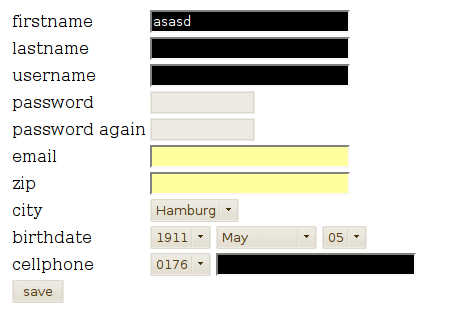
\includegraphics[scale=.6]{graphics/pico_reg_form.png}  
\end{figure}

I've changed the background color to black and the text to white just as
a test to see if the CSS was loading properly. Let's walk in order of
execution, first out is \textbf{main.l}:

\section{Walk through the \texttt{main.l} library}
\label{sec:registration-form}

\begin{wideverbatim}
(load "lib/http.l" "lib/xhtml.l" "lib/form.l" "lib/ps.l"
 "lib/adm.l" "lib/misc.l" "lib/rgx.l" "lib/tpl.l")
(setq *BP "projects/tpl-test/")
(setq *Css (pack *BP "css/styles.css"))
(load 
 (pack *BP "models/er.l") 
 (pack *BP "helpers/global-helpers.l"))

(de main () 
  (pool (pack *BP "db/test.db")))
    
(de start ()
  (app)
  (setq Tpl (new '(+Tpl) *BP))
  (assign> Tpl 'title "Registration Form")
  (parse> Tpl 'index)
  (compRun> Tpl)
  (out> Tpl))                  

(de go () 
   (server 8080 "@start"))
\end{wideverbatim}

So apart from the libraries we load \textbf{er.l} and \textbf{global-helpers.l},
\textbf{rgx.l} and \textbf{tpl.l} are the two libraries whose explanations I link to
above.

We load the database with pool initially because we start the server
with: \textbf{.p/ dbg.l projects/tpl-test/main.l -main -go.}

And go is of course responsible for starting the server on
\texttt{port 8080} and running start.

The start function will first start the session with app, create the
template object with our base path \texttt{*BP} and assign a title,
parse the template, compile it, run it and finally print it to the
browser.

Let's take a look at the template:

\begin{wideverbatim}
<html>
<head>
<title> <% get title %> </title>
<base href="<% bPath %>"/>
<link rel="stylesheet" href="<% path cssDir %>styles.css" type="text/css" >
</head>
<body>
<% gui reg-form %>
</body>
</html>
\end{wideverbatim}

There are some new things here since we went through the
\href{http://www.prodevtips.com/2008/07/17/templating-in-pico-lisp/}{template
  class}, but not much:

\begin{wideverbatim}
(dm path> (Var)
   (pack (srcUrl) (get This Var)))

(dm bPath> ()
   (baseHRef))
\end{wideverbatim}

The result could look like this:


\begin{wideverbatim}
<base href="http://localhost:44148/"/>
<link rel="stylesheet"
      href="http://localhost:8080/projects/tpl-test/css/styles.css" 
type="text/css" >
\end{wideverbatim}

So \texttt{baseHRef} outputs \href{http://localhost:44148}{http://localhost:44148} and
*srcUrl*\href{http://localhost:8080/}{http://localhost:8080/}, great. The reason for the base tag is
that the \href{http://software-lab.de/app.html}{GUI framework} needs it.
The port number keeps track of each session and is unique for that
nsession.


\section{Walk through the \texttt{er.l} library}
\label{sec:registration-form}

Before we start with the form itself let's go through the
\textbf{er.l} file and \textbf{global-helpers.l}, first \texttt{er.l}:

\begin{wideverbatim}
(extend +Entity)
(dm asSelect> ()
    (collect (: lbl) This NIL T (: lbl)))

(class +Member +Entity)
(rel fname    (+Need +Sn +Idx +String))
(rel lname    (+Need +Sn +Idx +String))
(rel uname    (+Need +Key +Sn +Idx +String))  #min 6 chars
(rel pwd      (+Need +String))                #min 6 chars
(rel zip      (+Need +Idx +String))           #min 5 chars, numerical
(rel city     (+Link)(+City))                 #lives in a city
# min 7 digits for validation but we store min 11 digits 
# (as is, no loc formatting)    
(rel cellnr   (+Need +Ref +String))  
# has to validate as proper email address
(rel email    (+Need +Key +Idx +String))     
(rel bdate    (+Need +Ref +Date))             #birthdate

\end{wideverbatim}

\begin{wideverbatim}

(class +CellPrefix +Entity)
# will be used in the registration to create a complete cell number
(rel nr (+Ref +String))
(var lbl . nr)

(class +City +Entity)
(rel nm (+Ref +String))
(var lbl . nm)
\end{wideverbatim}

We've got a link to \texttt{+City} in the \texttt{+Member}. The
\texttt{asSelect>} method is responsible for fetching a list to be
used as a drop down. In the \texttt{+CellPrefix} case it is
\textbf{nr} of course, and in the \texttt{+City} case it's
\textbf{nm}. Actually pretty redundant since they only have one
relation but that could quickly change.


\section{Walk through the \texttt{global-helpers.l} library}
\label{sec:registration-form}

\texttt{Global-helpers.l} contains some extra validation logic and
generators:

\begin{wideverbatim}
(class +Gh)

(dm range> (Start End Pad) 
    (make 
     (for (N Start (>= End N) (inc N)) (link (pad Pad N)))))
    
(dm getMonths> () 
    (range> This 1 12 2))

(dm getDays> () 
    (range> This 1 31 2))

(dm getYears> (Min-age)
    (let curYear (curYear> This) 
      (range> This (- curYear 100) (- curYear Min-age) 0 )))

(dm curYear> () (car (date (date))))
\end{wideverbatim}

Trivial stuff to generate various drop downs. Note \texttt{pad} to
get \texttt{01}, \texttt{02} etc.


\begin{wideverbatim}
(class +EmailField +TextField)
    
(dm chk> ()
  (ifn 
     (match> '+Rgx (super) '((word > 0) "{at}" (dmn > 0) "." (ltr > 2 < 5))) 
     ,"email-expected" 
     (super)))
    
(class +AlNum +TextField)

(dm chk> ()
  (ifn (alnum> '+Rgx (val> This)) ,"alnum-expected" (super)))
\end{wideverbatim}

So we create a new \texttt{+EmailField} and \texttt{+AlNum} based
on the basic \texttt{+TextField}. The main thing here is the
\texttt{chk>} method that is called automatically by the GUI logic
in order to check if a value is OK or not. The \texttt{+Rgx} stuff has
already been covered. Note the comma (\texttt{,}) It's a shortcut
for the localization logic, it will lookup the keys for translations
in translation files if they are provided, currently not though. Check
out the the
\href{http://www.prodevtips.com/2008/04/11/more-oo-in-pico-lisp/}{OO
  tutorial} for more info on \texttt{super} above, and
\texttt{extra} used below.


\begin{wideverbatim}
(class +MinLen)

(dm T (MinLen . @)
  (=: minLen MinLen)
  (pass extra))

(dm chk> ()
  (ifn 
     (>= (length (val> This)) (: minLen)) 
     (pack ,"minlen-1" (: minLen) ,"minlen-2") 
     (extra)))
\end{wideverbatim}

The minimum length logic, it does not inherit from something else but
is setup to work with other classes in a horizontal fashion. Note the
use of \texttt{,”minlen--1″ (: minLen) ,”minlen--2″}. We need this to
account for differing minimum lengths in the error message.

\begin{wideverbatim}
(class +PwdCheck)

(dm T (PwdGet . @)
  (=: pwdGet PwdGet)
  (pass extra))

(dm chk> ()
  (ifn (= (eval (: pwdGet)) (val> This)) ,"password-mismatch" (extra)))
\end{wideverbatim}

Also designed to be prefix class only. We simply check if the passwords
match.


\section{The registration form}
\label{sec:registration-form}

It's time for the registration form which is a biggie, I've uploaded it
\href{http://www.prodevtips.com/wp-content/uploads/2008/08/reg-form.l}{here}
if you want to see the whole thing at once. It will be chopped up below
in a from top to bottom fashion.

\begin{wideverbatim}
(action
    (let E (loc "*Err" err) 
       (set E (head 1 (val E))))
    (form NIL
       (unless *Post (=: obj (new! '(+Member))))
       (<table> NIL NIL NIL
          (<row> NIL ,"firstname" (gui '(+E/R +TextField)   
                '(fname : home obj) 10))
          (<row> NIL ,"lastname"  (gui '(+E/R +TextField) 
                 '(lname : home obj) 10))
          (<row> NIL ,"username"  (gui '(+E/R +MinLen +AlNum) 
                 '(uname : home obj) 6 10))
\end{wideverbatim}

Having everything be an argument to the action function is a requirement
for the GUI to work.

The first thing we do is override the default behavior of displaying
validation errors for all fields at once. We get the \texttt{*Err}
list from the err function defined in \texttt{form.l} line 207. After
that we extract and use the first error (if there are any).

The second thing we do is to build an empty \texttt{+Member} object
which will be available through \texttt{(: home obj)}. You might
notice the use of \textbf{new}!, what happens if the user just
navigates away you might think, there will be a lot of empty bullshit
in the database won't it? Sure, and they can be cleared out by running
a cron job every day or continuously although it consumes more
resources. Since we work with a new! object there will be no need for
future commits, from now on everything that happens happens on disk,
not memory.

We build the layout in a table where each call to
\texttt{\textless{}row\textgreater{}} will create new rows and tds.
Notice the calls to \texttt{gui}, apparently \texttt{+E/R} needs the
\texttt{‘(fname home obj)} list and \texttt{+TextField} the 10 number
(the size of the field).

Our first custom prefix classes comes in the form of \texttt{+MinLen}
and \texttt{+AlNum} which takes 6 and 10 respectively (remember that
+AlNum is just a \texttt{+TextField} with extra validation attached to
it).

\begin{wideverbatim}
(<row> NIL ,"password"       
   (gui 
      '(+E/R +PwdCheck +MinLen +PwField) 
      '(pwd : home obj) 
      '(val> (: home pwd2)) 6 10))
(<row> NIL ,"password again" (gui 'pwd2 '(+PwField) 10 ))
(<row> NIL ,"email" (gui '(+E/R +EmailField)       '(email : home obj) 10))
(<row> NIL ,"zip"   (gui '(+E/R +MinLen +NumField) '(zip : home obj) 6 10))
(<row> NIL ,"city"  (gui '(+E/R +TextField)        '(city : home obj) (asSelect> '+City)))
\end{wideverbatim}

Note that the code has been indented to save horizontal space, in
reality it's just a continuation of the above code.

\texttt{+PwdCheck} will work with \texttt{‘(val> (: home pwd2))} as
input, yes it's the value of the ``password again'' field.

The city \texttt{+TextField} will get the result of the \texttt{(asSelect>
‘+City)} call as it's input, note the lack of a quote (\textbf{‘}). So
we evaluate and get the list of cities which will turn the field into
a drop down instead of a normal text field.

\begin{wideverbatim}
(<row> NIL ,"birthdate" 
   (<div> 
      (gui '(+E/R +Fmt +Chart) '(bdate : home obj)
         '((Dat) (list (date Dat)))
         '((Lst) (and (caar Lst) (cadar Lst) (caddr (car Lst)) (date (car Lst))))
         3 )
      (gui 1 '(+TextField) (getYears> '+Gh 18))
      (gui 2 '(+Map +TextField)
         (make 
            (for (I . M) *MonFmt 
               (link (cons M I))))
         *MonFmt)
      (gui 3 '(+TextField) (getDays> '+Gh))))
\end{wideverbatim}

It's starting to get tricky. Remember that we use \texttt{+Date} for
the birth date so we need some way of getting it to prepopulate three
consecutive drop downs, and be inserted by getting the data in all of
them. Actually we are just updating the empty object we created at the
top all the time but insert might be a more proper wording since we
are replacing nothing with something.

The \texttt{+Fmt} is class will take care of getting and setting the
date, the first function \texttt{‘((Dat)\dots{})} will \texttt{set>}
and the second one \texttt{‘((Lst)\dots{})} will be our \texttt{val>}
function.

The \texttt{+Chart} prefix is responsible for handling our 3 date drop
downs and will therefore take 3 as its single argument. The
constituent gui elements need to know where they are in this list,
hence 1, 2 and 3 as the first argument. The second drop down will
display the months of the year by working with the global
\texttt{*MonFmt} which will contain the full names based on which
location we have selected. Since we haven't chosen a location they
will default to their English names. Come to think of it this piece of
code should have been put in global helpers since month drop downs are
pretty common.

\begin{wideverbatim}
(<row> NIL ,"cellphone" 
   (<div> 
      (gui '(+E/R +Chart) '(cellnr : home obj) 2 
         '((Str)
             (let Len 
                (length 
                   (Find '((P) (pre? P Str)) (asSelect> '+CellPrefix)))
                (setq Str (chop Str))
                (list 
                   (list (pack (cut Len 'Str)) (format (pack Str))))))
         '((Lst) (pack (caar Lst) (cadar Lst))))
      (gui 1 '(+TextField) (asSelect> '+CellPrefix))
      (gui 2 '(+MinLen +NumField) 7 10 )))
(<row> NIL (gui '(+Button) ,"save" '(url "@start"))))))
\end{wideverbatim}

Here we pass two extra set and get functions to the \texttt{+Chart}
class directly instead. The first one is needed due to the fact that
it will recieve for instance a string looking like
\texttt{01766587436}. It then needs to cut the string up to get a list
looking like this: \texttt{(0176 6587436)}, in order to repopulate on
for instance validation failure. The problem is that some mobile phone
prefix numbers can have five digits in Germany, ouch. That's why we
need to determine the length first, otherwise we could end up with the
wrong numbers.

Finally the \texttt{+Button} will post the form back to the start
function which in turn contains this function. The error logic at the
top of the form could be used to confirm a successful post by
displaying a new page or message. No error \texttt{==} success.


\title{Explicit Scope Resolution in PicoLisp}
\author{Henrik Sarvell}
% Use \authorrunning{Short Title} for an abbreviated version of
% your contribution title if the original one is too long
\institute{\texttt{hsarvell@gmail.com}}
%
% Use the package "url.sty" to avoid
% problems with special characters
% used in your e-mail or web address
%


\maketitle

\begin{abstract}
  This article describes how to use explicit scope resolution with
  \texttt{run} and \texttt{eval} when extending the \texttt{html}
  function with some arbitrary code as final argument. 
\end{abstract}

\section{Extending the \texttt{html} function}
\label{sec:expl-scope-res-extending-the-html}

Today I felt like extending the \textbf{html} function that is responsible for
rendering the bare bones of a HTML document in the GUI framework.

Normally a call to (\texttt{html}) looks something like:

\begin{wideverbatim}
(html 0 "Pico Admin" *CSS NIL
  (Some code here)
  (Some more code here) ... )
\end{wideverbatim}

The important thing is the fact that the function accepts some arbitrary
code(s) as the final argument. I wanted to simply hard code my stuff
into an ``extension'', like this:


\begin{wideverbatim}
(de pa-html Prg
  (html 0 "Pico Admin" *CSS NIL Prg))
\end{wideverbatim}

Calling the above is shorter than the original with the same arguments
over and over again and \texttt{Prg} is now the arbitrary code I
referred to above.

\section{ \texttt{FEXPR}s and scoping rules}
\label{sec:expl-scope-res-fexpr}


It wouldn't work though, what was going on? Well the answer is obvious
when you get some help and think a little about it. In our
\textbf{(pa-html)} above the \textbf{Prg} variable is a
\href{http://en.wikipedia.org/wiki/Fexpr}{FEXPR}; unevaluated code.
With our addition we add a new scope, the local scope of
(\texttt{pa-html}). It turns out that (\texttt{html}) doesn't expect
the code to come from this local scope, a lot of variables that are
defined in the scope calling (\texttt{pa-html}) are probably undefined
within the local scope of (\texttt{pa-html}) for instance. Hence the
massive crashing.

To understand the solution, let's start over from the beginning with the
\textbf{(up)} function:

\begin{wideverbatim}
(let Hello "Hello"
  (println Hello)
  (let Hello "Hi!"
     (println Hello)
     (let Hello "Greetings"
        (println Hello)
        (println (up Hello)))))
\end{wideverbatim}

Output:

\begin{wideverbatim}
"Hello"
"Hi!"
"Greetings"
"Hi!"
\end{wideverbatim}

So the call to (\texttt{up}) will check what \textbf{Hello} contained
in the scope above the scope that it was called in. In this case
``Hi!'' was the contents. If I say that the default value for
(\texttt{up}) is 1 you can probably figure out what the last
(\texttt{println}) would've printed had we passed it \texttt{(up 2
  Hello)} instead.


\section{Explicit scoping with  \texttt{run} and \texttt{eval}}
\label{sec:expl-scope-res-explicit-scoping-with-run}

\subsection{Using \texttt{run}}
\label{sec:expl-scope-res-using-run}

Both (\textbf{run}) and (\textbf{eval}) can accept a last optional
argument that will define their scope explicitly, let's start with
(\texttt{run}):


\begin{wideverbatim}
(de Lvl1 (Arg . Prg)
  (let Lvl "lvl: 1"
     (run Prg 1)))

(de Lvl2 ()
  (let Lvl "lvl: 2"
     (Lvl1 "some argument"
        (println Lvl) (println "Something more here") ) ) )
  
(Lvl2)
\end{wideverbatim}

Output:

\begin{wideverbatim}
"lvl: 2"
"Something more here"
\end{wideverbatim}

As you can see \textbf{(run Prg 1)} will run \textbf{Prg} within the scope of
(\textbf{Lvl2}), ``one up''. I think you can guess what the output would be if we
just did \textbf{(run Prg)}.

By this point you should be able to understand that


\begin{wideverbatim}
(de pa-html Prg
  (html 0 "Pico Admin" *CSS NIL (run Prg 1)))
\end{wideverbatim}

is how (\texttt{pa-html}) should look.


\subsection{Using \texttt{eval}}
\label{sec:expl-scope-res-using-eval}

Let's finish off with (\texttt{eval}) for good measure:

\begin{wideverbatim}
(de Lvl1 (Arg Lst)
  (let Lvl "lvl1"
     (eval Lst 1)))
  
(de Lvl2 ()
  (let Lvl "lvl2"
     (Lvl1 "I'm Arg" '(pack Arg " and I'm: " Lvl))))
  
(Lvl2)
\end{wideverbatim}

Output:

\begin{wideverbatim}
" and I'm: lvl2"
\end{wideverbatim}

Since \textbf{Arg} is undefined within the scope of (\textbf{Lvl2}) we
won't get ``I'm Arg'' in the beginning of the output. Just calling
\texttt{(eval Lst)} would of course result in “\texttt{I'm Arg and
  I'm: lvl1}″.

I think it's a bad idea to rely on explicit scope resolution out of
laziness, as you can imagine the code could easily become unintelligible
if not used sparingly. Use only when absolutely necessary if you can not
see any other solution.


\title{Pilog Solve and the +Aux Relation}
\author{Henrik Sarvell}
% Use \authorrunning{Short Title} for an abbreviated version of
% your contribution title if the original one is too long
\institute{\texttt{hsarvell@gmail.com}}
%
% Use the package "url.sty" to avoid
% problems with special characters
% used in your e-mail or web address
%


\maketitle


\begin{abstract}
  This article uses the 'Doctrine' example (known from the PHP world)
  to demonstrate the usage (and advantages) of Pilog \texttt{solve} and
  the \texttt{+Aux} relation. 
\end{abstract}

\section{'Doctrine for dummies' example}
\label{sec:pilog-solve-'doctrine-for-dummies'-example}


I just set out to duplicate the
\href{http://www.prodevtips.com/2008/08/05/doctrine-for-dummies/}{Doctrine
  for dummies example}, but this time for real, with a real OODB
system, not some silly ORM. Thanks goes to Alex for helping me out with
the queries.


\begin{wideverbatim}
(class +Member +Entity)
(rel uname  (+Need +Key +String))
(rel pwd    (+Need +String))
(rel email  (+String))
(rel city   (+Ref +Link) NIL (+City))

(class +City +Entity)
(rel name   (+Key +String))

(class +Message +Entity)
(rel subject (+Idx +String))
(rel body    (+String))
(rel from    (+Ref +Link) NIL (+Member))
(rel to      (+Aux +Ref +Link) (from) NIL (+Member))

(pool "dbtest.db")
\end{wideverbatim}

So we create the relations, and the database file. Take special note of
the \textbf{+Aux} relation from \textbf{to} to \textbf{from}. It will play a central role
later.


\begin{wideverbatim}
(setq Mbrs 
  (list
     (list "member1" "password1" "member1@members.com" "Berlin")
     (list "member2" "password2" "member2@members.com" "Stuttgart")
     (list "member3" "password3" "member3@members.com" "Hamburg")))
  
(for Mbr Mbrs
  (request '(+Member) 
     'uname (get Mbr 1) 
     'pwd   (get Mbr 2) 
     'email (get Mbr 3) 
     'city  (request '(+City) 'name (get Mbr 4))))
\end{wideverbatim}

We input some members in the database, note the use of \textbf{request}. The
major thing is that it will create an object if there is none with the
given key(s) already, however if there is an object with the given keys
it will return that object, quite handy.


\begin{wideverbatim}
(setq Mbr1 (db 'uname '+Member "member1"))
(setq Mbr2 (db 'uname '+Member "member2"))

(new T '(+Message) 
  'subject "from mbr1 to mbr2"
  'body "Hello mbr2 this is mbr1"
  'to Mbr2
  'from Mbr1)
  
(new T '(+Message) 
  'subject "from mbr2 to mbr1"
  'body "Hello mbr1 this is mbr2"
  'to Mbr1
  'from Mbr2)
  
(new T '(+Message) 
  'subject "from mbr2 to mbr1, again"
  'body "Hello mbr1 this is mbr2, again"
  'to Mbr1
  'from Mbr2)
  
\end{wideverbatim}

\begin{wideverbatim}

(new T '(+Message) 
  'subject "from mbr1 to mbr3"
  'body "Hello mbr3 this is mbr1"
  'to (db 'uname '+Member "member3")
  'from Mbr1)
  
(commit)
\end{wideverbatim}

Note the use of \textbf{(new T\dots{})} without the \texttt{T} we won't
get database objects.


\section{Querying}
\label{sec:pilog-solve-querying}

\subsection{Simple queries}
\label{sec:pilog-solve-simple-queries}

\begin{wideverbatim}
(mapc show (collect 'to '+Message Mbr1 Mbr1 'from))
(mapc show (collect 'from '+Message Mbr1 Mbr1 'to))
(mapc show (collect 'from '+Message Mbr1 Mbr1))
(mapc show (collect 'to '+Message Mbr1 Mbr1))
\end{wideverbatim}

Test that everything is there by calling the above statements, the first
one will get all people who sent a message to member 1. The second one
will instead get all people who member 1 sent messages to. The two last
ones will do the same but will get messages, not people. And that was
that, this is as complex as the PHP Doctrine example got, let's move on
to more complex stuff relating to the +Aux relation:

\subsection{Using the \texttt{+Aux} relation}
\label{sec:pilog-solve-using-the-+aux}

\begin{wideverbatim}
(scan (tree 'to '+Message))
(scan (tree 'from '+Message))
\end{wideverbatim}

Output:

\begin{wideverbatim}
({5} {:} . {H}) {H}
({5} {:} . {I}) {I}
({:} {5} . {B}) {B}
({A} {5} . {L}) {L}

({5} . {B}) {B}
({5} . {L}) {L}
({:} . {H}) {H}
({:} . {I}) {I}
-> {F}
\end{wideverbatim}

Notice the difference, the \textbf{to} relation is utilizing \textbf{+Aux} so we have
extra references there between the message receiver and sender. Together
the combination can be used as a key to speed up things.


\begin{wideverbatim}
(mapc show (collect 'to '+Message (list Mbr1 Mbr2)))
\end{wideverbatim}

This is an example of how to use the \texttt{+Aux} relation to get all messages
to member 1 from member 2 with \textbf{collect}.


\subsection{Pilog \texttt{solve} with parallel scanning}
\label{sec:pilog-solve-using-the-+aux}

\begin{wideverbatim}
(mapc show
   (solve  
     (quote @M1 Mbr1 @M2 Mbr2 @S "mbr2" 
        (select (@Msgs) 
           ((subject +Message @S) (to +Message @M1) (from +Message @M2))
           (same @M1 @Msgs to)
           (same @M2 @Msgs from)
           (tolr @S @Msgs subject)))  
     @Msgs ))
\end{wideverbatim}

The above code will retrieve all messages from member 2 to member 1
that also contain the word “\texttt{mbr2}″ in the subject. It is
however not using the \texttt{+Aux} relation to make the lookup of who
is sending a message to who, we scan in parallel here.


\subsection{Pilog \texttt{solve} using the \texttt{+Aux} relation}
\label{sec:pilog-solve-using-the-+aux}


\begin{wideverbatim}
(mapc show 
   (solve
      (quote
         @M1 Mbr1
         @M2 Mbr2
         @M (list Mbr1 Mbr2)
         @S "mbr2"
         (select (@Msgs)
            ((subject +Message @S) (to +Message @M))
            (tolr @S @Msgs subject)
            (same @M1 @Msgs to)
            (same @M2 @Msgs from))) 
      @Msgs ))
\end{wideverbatim}

This example is however using the \texttt{+Aux} relation. The
\textbf{@M} list will look for for example the \textbf{\{5\} \{:\}}
combo above in the \textbf{(to +Message @M)} clause. Next we filter as
usual.

After benchmarking the above examples I got a 3\% speed increase in favor
of the second one using 6000 messages to test on, when using 11000 the
difference increased to 11\% so careful planning will pay off more and
more the bigger the database becomes.

\title{PicoLisp and JSON}
\author{Henrik Sarvell}
% Use \authorrunning{Short Title} for an abbreviated version of
% your contribution title if the original one is too long
\institute{\texttt{hsarvell@gmail.com}}
%
% Use the package "url.sty" to avoid
% problems with special characters
% used in your e-mail or web address
%


\maketitle


\begin{abstract}
This article discusses libraries and tests for converting PicoLisp to
JSON and vice versa.   
\end{abstract}

\section{Introduction}
\label{sec:pl-json-introduction}

Yet again I have to do some documenting so I know what the hell I'm
doing since I'm all over the place at the moment. Doing something here
and then moving over to do something over there and then coming back to
coding this and that. If you're this unstructured you need crutches and
this documentation is that, it will enable me to get back to this and do
easy debugging in the future, it will trigger memories.

Therefore this code is very rough and untested, a work in progress, you
have been warned\dots{}

If you somehow landed on this page without any background on PicoLisp
or Lisp you probably need to start
\href{http://www.prodevtips.com/2008/03/28/pico-lisp/}{from the beginning}.

\section{The tests}
\label{sec:pl-json-the-tests}

\subsection{PicoLisp to JSON}
\label{sec:pl-json-picolisp-to-json}

Let's start with the tests for a change. This is an example of
converting a proper database object to JSON. The code will determine the
relations and use them to build the JSON, nothing else that might be in
there:


\begin{wideverbatim}
(load "lib/str.l")
(load "lib/json.l")

(class +Product +Entity)
(rel name (+Need +String))
(rel id (+Need +Number))
(rel descr (+String))
(rel attributes (+List +String))

(setq Product
   (new '(+Product) 'name
      "A \"PC\"" 'id 123 'attributes '("black" "laptop") ) )

(println (to> '+Json 'encObj> Product))
\end{wideverbatim}

Output:

\begin{wideverbatim}
  "{\"attributes\": [\"black\", \"laptop\"], \"id\": 123,
    \"name\": \"A \\\"PC\\\"\", \"descr\": false}"
\end{wideverbatim}

\textbf{Associative structure}, it will also be encoded as object:

\begin{wideverbatim}
(setq Pairs '((key1 . hello) (key2 . world) (false . NIL)
              (someArr . (1 2 "hello quote: \"quote\"" 4)) ) )
(println (to> '+Json 'encPair> Pairs))
\end{wideverbatim}


\begin{wideverbatim}
  "{\"key1\": \"hello\", \"key2\": \"world\", \"false\": false,
    \"someArr\": [1, 2, \"hello quote: \\\"quote\\\"\", 4]}"
\end{wideverbatim}

\textbf{2D structure} will be an array of objects:

\begin{wideverbatim}
(setq Pair1 '((key1 . hello) (key2 . world) (false . NIL) (someArr . (1 2 "hello" 4))))
(setq Pair2 '((key1 . hello) (key2 . world) (false . NIL) (someArr . (1 2 "world" 4))))
(setq Tst (list Pair1 Pair2))
(println (to> '+Json 'encTable> Tst))
\end{wideverbatim}


\begin{wideverbatim}
  "[{\"key1\": \"hello\", \"key2\": \"world\", \"false\": false,
    \"someArr\": [1, 2, \"hello\", 4]}, 
  {\"key1\": \"hello\", \"key2\": \"world\", \"false\": false,
    \"someArr\": [1, 2, \"world\", 4]}]"
\end{wideverbatim}

Simple case of \textbf{nested list}:

\begin{wideverbatim}
(setq Tst (list 1 2 "hello" (1 2 3) 3 4 "world"))
(println (to> '+Json 'encArr> Tst))
\end{wideverbatim}


\begin{wideverbatim}
"[1, 2, \"hello\", [1, 2, 3], 3, 4, \"world\"]"
\end{wideverbatim}

\subsection{JSON to PicoLisp}
\label{sec:pl-json-json-to-picolisp}

\begin{wideverbatim}
(setq Json "{\"hello1\": {\"subObj\": [123, 456, true, NIL]}, \"b\": true}")
(setq Result (from> '+Json Json))
(show Result)
(show (get Result 'hello1))
\end{wideverbatim}


\begin{wideverbatim}
$385543015 NIL
   b
   hello1 $385543062
$385543062 NIL
   subObj (123 456 T NIL)
\end{wideverbatim}

\section{The library}
\label{sec:pl-json-the-library}


\subsection{JSON to PicoLisp}
\label{sec:pl-json-json-to-picolisp}



\begin{wideverbatim}
(class +Json)

(dm from> (J)
  (=: L (chop J))
  (let C (pop (:: L))
     (let R (if (= C "[") (pre> This 'pArr>) (pre> This 'pObj>))        
        (parse> This R))))
\end{wideverbatim}

This is where the coding from JSON to PicoLisp structure begins.


\begin{wideverbatim}
(dm pre> (Type)
  (let (R (list Type) InStr NIL)
     (catch NIL 
        (while (: L)
           (let C (pop (:: L))
              (cond
                 ((= C "[") (queue 'R (pre> This 'pArr>)))
                 ((= C "{") (queue 'R (pre> This 'pObj>)))
                 ((and (or (= C "]") (= C "}")) (nT InStr)) (throw))
                 (T (when (= C "\"") 
                          (setq InStr (not InStr))) 
                       (queue 'R C)))))) R ))
\end{wideverbatim}

Here we are creating an intermediary list that will be easy to
execute. We do this by inserting the names of functions to use in
later steps into this list. But what is really happening? Well as you
saw from the prior listing we begin with either
\textbf{pArr\textgreater{}} or \textbf{pObj\textgreater{}} depending
on if we are to begin parsing to an object or an array. \textbf{InStr}
will keep track of whether the characters \textbf{\{, \}, [, ]} are
inside a string or not, if they are they should not count of course.

So while we still have characters in our chopped up list we will loop
through them by destructively popping, if we have a ``[`` we will put
\textbf{pArr\textgreater{}} on the list instead of the caracter, if we
have ``\{'' we put \textbf{pObj\textgreater{}}. If we have the
respective closing character, and it is not inside a string, we exit
by throwing \texttt{NIL}.


\begin{wideverbatim}
(dm any> (L)
   (let R (any (pack L))      
      (if (= R "true") T (if (= R "false") NIL R))))

(dm parse> (L)  
  (apply (car L) (list This (cdr L))))
    
(dm pObj> (L)
  (let (R (new) L (split L ",")) 
     (for El L
        (let Pair (split El ":")
           (put R 
              (any (any (pack (car Pair)))) 
              (let Value (cdadr Pair)                 
                 (if (lst? (car Value))
                    (parse> This (car Value))
                    (any> This Value)))))) R ))
\end{wideverbatim}

We begin by applying either \textbf{pObj\textgreater{}} or
\textbf{pArr\textgreater{}} in \textbf{parse\textgreater{}}.

The \texttt{pObj>} method will begin with creating the empty result
object, \textbf{R} and a list of sublists looking something like this:
(``k'' ``e'' ``y'' ``:'' ``v'' ``a'' ``l'' ``u'' ``e'') in \textbf{L} by
splitting by ``,''.

We continue by splitting by ``:'' to get the key and the value. The key is
then retrieved, the value will be further examined to determine if we
should apply recursion to get a sub-object/array or simply return the
result through \textbf{any\textgreater{}}.

\begin{wideverbatim}
(dm pArr> (L)
   (make       
      (for El (mapcar 'clip (split L ","))         
         (if (lst? (car El))
            (link (parse> This (car El)))
            (link (any> This El))))))
\end{wideverbatim}


\subsection{PicoLisp to JSON}
\label{sec:pl-json-picolisp-to-json}


\begin{wideverbatim}
(dm to> (F L)
   (pack (make (apply F (list This L)))))
\end{wideverbatim}

As you know from the tests above the behavior has to be explicitly set
by passing the function name to be used to generate the result when
going from PicoLisp to Javascript. It's pretty obvious actually since
it's impossible to determine from the structure of various types of
lists how to treat them. We can't infer whether a list is a normal
nested list or a paired list, for all intents and purposes they are
identical. However the output will be radically different. Note
\textbf{make}, that is why we are able to use \textbf{link} all over
the place below.


\begin{wideverbatim}
(dm encTable> (Tbl)
  (link "[")
  (let F T 
     (mapc 
        '((L) 
            (link (comma> This F)) 
            (encPair> This L) 
            (setq F NIL)) Tbl))
  (link "]"))

(dm encPair> (L)    
  (link "{")
  (let F T 
     (mapc 
     '((El) 
         (link (pack (comma> This F) "\"" (car El) "\"" ":" " "))
         (setq F NIL)                  
         (enc> This (if (pair El) (cdr El) NIL))) L ))
  (link "}"))

(dm comma> (First)
   (unless First ", "))
\end{wideverbatim}

Some redundant code here, it might benefit from refactoring, or we
could just leave it like it is and call it a day, yeah let's do that.
When encoding a table each element will in turn be encoded with
\textbf{encPair\textgreater{}}, if we have the first element we do not
prepend the ``,''.

A paired list will be encoded as an object with
\textbf{encPair\textgreater{}}.


\begin{wideverbatim}
(dm encArr> (L)  
  (link "[")
  (let F T
     (mapc 
     '((El) 
         (link (pack (comma> This F)))
         (setq F NIL)
         (enc> This El)) L ))
  (link "]"))
\end{wideverbatim}

Redundancy again! \texttt{List -> array} is easier though than
\texttt{paired list -> object}.


\begin{wideverbatim}
(dm encObj> (O)
  (encPair> This 
     (make 
        (mapc 
           '((Prop)
               (when (isa '+Relation (car Prop)) 
                  (let Key (cdr Prop) 
                     (link (cons Key (get O Key)))))) (getl (car (type O)))))))
\end{wideverbatim}

Finally something clever, in case of object we will get all the
properties of the object through the \texttt{getl} function. Every
property that is a relation will get the ``treatment''. We get the
name of the relation as \textbf{Key} and use that name on the original
object to retrieve the value. The resultant array is now a paired list
that can be encoded with \textbf{encObj\textgreater{}}.


\begin{wideverbatim}
(dm enc> (L)   
   (cond 
      ((=T L)    (link "true"))
      ((not L)   (link "false"))

      ((num? L)  (link L))
      ((lst? L)  (encArr> This L))
      ((or (box? L) (ext? L)) (encObj> This L))))
\end{wideverbatim}

accordingly, notice the escaping with \textbf{+Str}. It's the genesis of some
kind of general string library, not much in there yet though:

\begin{wideverbatim}

(dm fChr> (Lst Chr)
  (find '((C)(= C Chr)) Lst))
   
#S = hello, Lst = '("\"")
(dm esc> (S Lst)
  (pack 
     (mapcar 
        '((C)
            (if (fChr> This Lst C) (pack "\\" C) C )) (chop S))))
\end{wideverbatim}

Every character in the passed list (in this case only one) will be
escaped.


% \title{PicoLisp to JSON with JavaScript}
\author{Henrik Sarvell}
% Use \authorrunning{Short Title} for an abbreviated version of
% your contribution title if the original one is too long
\institute{\texttt{hsarvell@gmail.com}}
%
% Use the package "url.sty" to avoid
% problems with special characters
% used in your e-mail or web address
%


\maketitle

\begin{abstract}
  This article describes how to convert PicoLisp to JSON on the client
  side instead of on the server, using JavaScript.  
\end{abstract}

\section{REGEXP problems}
\label{sec:pl-json-jscript-regexp-problems}

On many occasions it's preferable to convert PicoLisp on the client side
instead of on the server, here's an attempt.

However, there are two problems with the below approach:

\begin{enumerate}
\item The first huge regexp that checks for a paired list will break
  if any key or value has an escaped quote in it. I've scoured the
  Internet until my eyes bled but I couldn't find an example of
  JavaScript regex that would handle backslashes. I also found out
  that the JS regexp capabilities are not 100\% on par with for
  instance PERL's, it might be what what I want is impossible to
  achieve with regexes alone.
\item The second regexp that checks for a single pair/obj will not
  work if the key has an escaped quote in it, this is however a less
  serious problem than 1) as it's extremely unlikely to happen.
\end{enumerate}

\textbf{Update}: I've gotten some help from Mateusz Jan Przybylski on the
\href{http://www.mail-archive.com/picolisp@software-lab.de/msg01050.html}{PicoLisp mailing list}. It seems we can handle quotes in the values of objects
now. I still couldn't get it to work though with the standalone, single
pair/object so \#2 above still holds.

\textbf{Update 2:}: After some discussion on the mailing list again
we've agreed to handle \texttt{(”:key” (1 2 3))} as \texttt{\{”key”:
  [1, 2, 3]\}}. This current version is more flexible than what you've
seen here before, it will now handle nested associative lists. It is
however not very robust, I can think of a lot of strange edge
scenarios that will make it break. Anyway, it's good enough for me and
my current usage scenarios.

\section{JavaScript Code}
\label{sec:pl-json-jscript-javascript-code}

\begin{wideverbatim}
function countSubsChrs(str, start_chr, pos, dir){
    var cur_chr = start_chr;
    var count   = 0;
    while(cur_chr == start_chr){
      cur_chr   = str.charAt(pos);
      pos       += dir;
      count     += 1;
    }
    return count;
}

function isEscaped(str, pos){
    var result = countSubsChrs(str, '\\', pos, -1) % 2;
    return result == 0 ? false : true;
}

function getListEnd(str, cur_pos, dir){
    var lvl = 1;
    var pos = cur_pos + dir;
    var dq  = 0;
    while(lvl != 0 && pos != str.length){
        var chr = str.charAt(pos);
        switch(chr){
            case '"':
                if(!isEscaped(str, pos)) dq += 1;
                break;
            case '(':
                if(dq % 2 == 0) lvl += dir;
                break;
            case ')':
                if(dq % 2 == 0) lvl -= dir;
                break;
            default: break;
        }


\end{wideverbatim}

\begin{wideverbatim}

        if(pos < 1) break;
        pos += dir;
    } 
    return pos; 
}

function isPaired(str){
    var is_p = true;
    if(str.match(/^\(.+\)$/)){  
        for(var i = 0; i < str.length; i++){
            if(str.charAt(i) == '('){
                var rest = str.slice(i+1);
                if(!rest.match(/^"\:[^"]*"\s\(/) && 
                   !rest.match(/^("[^"]*"|\d+)\s\.\s[^\s]/)){
                    is_p = false;
                    break;
                }
                i = getListEnd(str, i, 1) - 1;
            }
        }
    }else
        is_p = false;
    return is_p;
}

function hasKey(str, pos){
    var back_str = str.slice(getListEnd(str, pos, -1) + 2, pos);
    return back_str.match(/^("\:[^"]*")\s/);
}

function picoToJson(str){
    str = str.slice(1, -1);
    
    if(isPaired(str))
        var mode = 'pairs';
    else if(str.match(/^"\:[^"]*"\s/))
        var mode ='obj';
    else
        var mode = str.match(/^("[^"]*"|\d+)\s\.\s[^\s]/) ? 'obj' : 'arr';
    
    var rstr = mode == 'arr' ? "[" : "{";
    var is_str = false;
    var chr = "";


\end{wideverbatim}

\begin{wideverbatim}


    for(var i = 0; i < str.length; i++){
        chr = str.charAt(i);
        if(is_str){
            if(str.charAt(i) == ':' && (str.charAt(i-2) == 
            '(' || str.charAt(i-1) == '"') && (mode == 'obj' || mode == 'pairs'))
                rstr += '';
            else
                rstr += chr;
            if(chr == '"' && str.charAt(i - 1) != '\\')
                is_str = false;    
        }else{
            switch(chr){
                case '(':
                    if(mode != 'pairs'){
                        var end_pos = getListEnd(str, i, 1);
                        rstr += picoToJson( str.slice(i, end_pos));
                        i = end_pos - 1;
                    }else{
                        if(i != 0 && str.charAt(i-2) != ')'){
                            if(hasKey(str, i)){
                                var end_pos = getListEnd(str, i, 1);
                                rstr += picoToJson( str.slice(i, end_pos) );
                                i = end_pos - 1;
                            }
                        }
                    }   
                    break;
                case 'N':
                    if(str.charAt(i+1) == 'I' && str.charAt(i+2) == 'L'){
                        rstr += 'false';
                        i += 2;
                    }
                    break;
                case 'T':
                        rstr += 'true';
                    break;
                case ')':
                    if(i < str.length - 1)
                        rstr += ',';
                    break;
                case '"':
                    if(str.charAt(i - 1) != '\\')
                        is_str = true;
                    rstr += chr;
                    break;


\end{wideverbatim}

\begin{wideverbatim}


                case ' ':
                    if(str.charAt(i + 1) == '(' && (mode == 'obj' || mode == 'pairs')){
                        if(mode == 'obj')
                            rstr += ": ";
                        else if(mode == 'pairs' && str.charAt(i-1) != ')')
                            rstr += ": ";
                        else
                            rstr += " ";
                    }else if(str.charAt(i + 1) == '.' &&
                            (mode == 'obj' || mode == 'pairs')){
                        rstr += ":";
                        i++;
                    }else if(mode == 'arr')
                        rstr += ', ';
                    else
                        rstr += chr;
                    break;
                default:
                    rstr += chr;
                    break;
            }
        }
    }
    rstr += mode == 'arr' ? "]" : "}";
    return rstr;
}

function evalPico(str){
    return eval('('+picoToJson(str.replace(/\n/gm, ''))+')');
}

var str = '("first element" ("obj" . "yes") 2 
           (":links" (1 2 3)) ((1 . 2) (":links" (4 5 6))) "final element")';
var json = picoToJson(str);
alert(json);
var result = eval('('+json+')');
alert(result[3].links.pop());
\end{wideverbatim}

A lot of the code above has been converted from the Ruby
\href{http://www.prodevtips.com/2008/05/06/scintilla-basics-in-wxruby/}{Pico
  Editor} code.



\title{Factorials, Permutations and Recursion in PicoLisp}
\author{Henrik Sarvell}
% Use \authorrunning{Short Title} for an abbreviated version of
% your contribution title if the original one is too long
\institute{\texttt{hsarvell@gmail.com}}
%
% Use the package "url.sty" to avoid
% problems with special characters
% used in your e-mail or web address
%


\maketitle

\begin{abstract}
  This article describes \emph{factorials}, \emph{permutations} and
  \emph{recusrion} can be used in the simulation of stock trading
  strategies.  
\end{abstract}

\section{Simulating stock trading strategies}
\label{sec:fact-perm-recur-simulating-stock-trading-strategies}

Currently I'm simulating trading strategies on historical stock data.
Yes I know according to
\href{http://en.wikipedia.org/wiki/Nassim_taleb}{Nassim} this is
complete bullshit but I might beg to differ. At least I feel the need
to determine if it's bullshit on my own than just take his word for it.

I have bought trading data from the SET which includes the years
1975--2008, the period 1997--2001 could possibly closely resemble what
we are up against at the moment so any simulated strategy that returns
more than simply sitting on the sidelines and doing nothing is a winner
and might be worth testing at the moment.

\section{Factorials and Permutation}
\label{sec:fact-perm-recur-factorials-and-permutation}


\subsection{First try}
\label{sec:fact-perm-recur-first-try}

However in order to simulate these strategies we need to be able to do
permutations and I couldn't find anything already created to this
effect, neither could I find a core factorial function, so here they
are:

\begin{wideverbatim}
(de fac (Num)
   (let Res 1
      (for (N 1 (>= Num N) (inc N))
         (setq Res (* Res N)))))
\end{wideverbatim}

So this one is basically the same as ye old ``N!''.

\begin{wideverbatim}
(de switch (Lst P1 P2)
  (let (V1 (get Lst P1) V2 (get Lst P2))      
      (place P1 (place P2 Lst V1) V2)))
\end{wideverbatim}

This one is used in the permutate function below, however it might be of
use in a standalone fashion, hence it having its own definition. Anyway
the end result is a switch of the values indicated by the numbers in P1
and P2.

\subsection{Using \texttt{recur} and \texttt{recurse}}
\label{sec:fact-perm-recur-using-recur}

\begin{wideverbatim}
(de permutate (Lst)      
   (let (Result (list) Count 1 Start 1) 
      (recur (Lst Start Result Count) 
         (when (>= (fac (length Lst)) Count)
            (push Result Lst)
            (when (= Start (length Lst)) (setq Start 1))
            (recurse 
               (switch Lst Start (inc Start)) 
               (inc Start) 
               Result 
               (inc Count)))
         (car Result))))
\end{wideverbatim}

Note \textbf{recur} and \textbf{recurse} here, we might just have
created a different non-recursive entry function instead but using
these two is a more lazy approach that lets us dispense with the need
to create two different definitions.

The end result is a list of lists with all different permutations.

Anyway, I will put this stuff up for inspection on the Pico Lisp mailing
list and let more knowledgeable people give feedback, updates with new
code and comments will most likely appear here in the near future. 

\textbf{Update}: OK so it didn't work, I created the above based on an
(1 2 3) example list, however in my sharp application I work with 4
numbers and it didn't manage that, I'll leave it though as an example
of how recursion can be done in PicoLisp.

\subsection{Second try}
\label{sec:fact-perm-recur-second-try}

I ended up stealing one of the algorithms from the
\href{http://en.wikipedia.org/wiki/Permutation}{permutation Wikipedia}
article, and this is the result:


\begin{wideverbatim}
(de permutation (N Lst)
   (for (J 2 (>= (length Lst) J) (inc J))
      (setq N (/ N (- J 1)))
      (setq Lst (switch Lst (inc (% N J)) J))))
   
(de permutate (Lst)
   (let Rslt (list)
      (for (N 1 (>= (fac (length Lst)) N) (inc N))
         (push Rslt (permutation N Lst)))
      (uniq (car Rslt))))
\end{wideverbatim}

Everything else equal.

\subsection{Using \texttt{permute}}
\label{sec:fact-perm-recur-using-permute}

\textbf{Update}: So I got my answer from Alex on the mailing list:

\begin{quote}
Well, there is the `permute' function in ``lib/simul.l''. Does it what
you intend?
\end{quote}


\begin{wideverbatim}
(de permute (Lst)
   (ifn (cdr Lst)
      (cons Lst)
      (mapcan
         '((X)
            (mapcar
               '((Y) (cons X Y))
               (permute (delete X Lst)) ) )
         Lst ) ) )
\end{wideverbatim}

Indeed, and very nice, excellent solution, I wish my mind was lispy
enough to come up with these things myself. If you encapsulate the
recursive permute call in a println you will get a feeling for how it
works.

\title{Prolog as a Dating Aid}
\author{Henrik Sarvell}
% Use \authorrunning{Short Title} for an abbreviated version of
% your contribution title if the original one is too long
\institute{\texttt{hsarvell@gmail.com}}
%
% Use the package "url.sty" to avoid
% problems with special characters
% used in your e-mail or web address
%


\maketitle


\begin{abstract}
  This article describes how \texttt{Pilog}, PicoLisp's implementation
  of \texttt{Prolog}, can be used to find out which women in a
  flirt\&dating database have similar tastes like the male
  candidate. 
\end{abstract}

\section{A \texttt{Prolog} presentation}
\label{sec:prolog-dat-aid-a-prolog-presentation}

This Saturday I had a small presentation. It wasn't really well prepared
so I'll try and make up for it here instead.

I wanted to demonstrate how Prolog, or in my case Pilog (same thing but
different syntax), could be used to solve problems and query object
databases. If you've been following my stuff on PicoLisp you won't find
much new.

\section{Set up a Prolog environment}
\label{sec:prolog-dat-aid-set-up-a-prolog-environment}

First I began by setting up a simple Prolog environment to demonstrate
how Pilog can be used in a setting free of object databases. The goal is
to find a compatible woman. This is basically the same thing as the
\href{http://www.prodevtips.com/2008/04/28/advanced-oodb-in-pico-lisp/}{food example}.


\begin{wideverbatim}
(be actionMovies (Jane))
(be actionMovies (Yoko))
(be durian (Kwan))
(be somTum (Kwan))
(be diving (Anna))
(be Japanese (Yoko))
(be blond (Anna))
(be petite (Yoko))
(be petite (Kwan))
(be sporty (Anna))
(be funny (Yoko))
(be likeBeer (Jane))
(be likeBeer (Anna))
(be speaksThai (Kwan))

(be likes (Tum @F) (actionMovies @F))
(be likes (Tum @F) (Japanese @F))
(be likes (Tum @F) (blond @F))
(be likes (Tum @F) (petite @F))
(be likes (Tum @F) (funny @F))
(be likes (Tum @F) (sporty @F))
(be likes (Tum @F) (likeBeer @F))
(be likes (Tum @F) (speaksThai @F))
(be likes (Tum @F) (durian @F))
(be likes (Tum @F) (somTum @F))
(be likes (Tum @F) (diving @F))

(let L NIL
        (solve '((likes Tum @F))
           (accu 'L @F 1) )
        (flip (by cdr sort L)) )

(println L)
\end{wideverbatim}

The last sequence will output the woman Tum likes the most first and
then in descending order. Try to fool around with it, starting with
\texttt{(? (likes Tum @F))} and then adding the rest step by step and
see how the output changes for each step.

\section{The database}
\label{sec:prolog-dat-aid-the-database}


\subsection{Generate the database}
\label{sec:prolog-dat-aid-generate-the-database}

Let's move on to the database stuff. First we need to generate it, you
can do that by running the following:


\begin{wideverbatim}
(class +Woman +Entity)
(rel id       (+Key +Number))
(rel age      (+Number))
(rel country  (+Ref +Link) NIL (+Country))
(rel hair     (+Ref +Link) NIL (+Color))
(rel smoking  (+Number))
(rel tattoo   (+Number))

(class +Country +Entity)
(rel name (+Key +String))

(class +Color +Entity)
(rel color (+Key +String))

(class +Likes +Entity)
(rel name  (+Key +String))

(class +LikesCon +Entity)
(rel woman  (+Aux +Ref +Link) (likes) NIL (+Woman))
(rel likes  (+Ref +Link) NIL (+Likes))
 
(pool "bcamp_phuket.db")

(de randEls (Cls Key Amount)
   (make 
      (let Lst (collect Key Cls)         
         (do Amount
            (let Nth (rand 1 (length Lst))               
               (link (get Lst Nth)))))))
    
\end{wideverbatim}

\begin{wideverbatim}

(de setup()
   (mapc '((Col) (new!  '(+Color)   'color Col))
      '("red" "brown" "blond" "black") )
   (mapc '((Like)(new!  '(+Likes)   'name Like))
      '("diving" "skiing" "partying" "pop" "rock" "alternative" "cars"
          "beer" "tennis" "wine" "golf" "geeks" "computers" "som tam"
          "gaeng som" "larb moo" "gaeng aum" ) )
   (mapc '((Con) (new!  '(+Country) 'name Con))
      '("Sweden" "Thailand" "Japan") ) )

(de createWomen ()
   (let N 0 
      (do 10000
         (new! '(+Woman) 
            'age (rand 18 65)
            'country (car (randEls '+Country 'name 1))
            'hair (car (randEls '+Color 'color 1))
            'smoking (rand 0 1)
            'tattoo (rand 0 1)
            'id (inc 'N)))))
    
(de createLikes ()
   (for W (collect 'id '+Woman)
      (for L (randEls '+Likes 'name 10)
         (new! '(+LikesCon) 'woman W 'likes L))))
    
(setup)
(createWomen)
(createLikes)
\end{wideverbatim}

This example uses \textbf{new!}, it takes quite a while to generate
the database like this. You could try \textbf{new} followed by a
\textbf{commit} when all the objects have been created if you want
this to go faster.


\subsection{Query the database}
\label{sec:prolog-dat-aid-query-the-database}

Let's move on to the final piece, you run this after the above code,
don't forget to delete the three last function calls or comment them out
first. The end could look like this:


\begin{wideverbatim}
#(setup)
#(createWomen)
#(createLikes)

(setq Start (usec))
(setq Women
   (uniq 
      (mapcar '((Con)(; Con woman)) 
         (solve   
            (quote
               @C1 "Japan"
               @C2 "Thailand"
               @L1 "beer"         
               @L2 "diving"         
               @L3 "geeks"         
               @Tat 1
               @Smo 0
               (select (@Links)  
                  (((name +Likes @L1 name +Likes @L2 name +Likes @L3) (likes +LikesCon)))
                  (or
                     ((same @C1 @Links woman country name))
                     ((same @C2 @Links woman country name)))
                  (same @Tat @Links woman tattoo)
                  (same @Smo @Links woman smoking)))   
            @Links ))))
    
(setq End (format (/ (- (usec) Start) 100000) 1))

(mapc 
   '((W)
       (println 
          (; W country name)           
          (; W smoking)          
          (; W tattoo)          
          (collect 'woman '+LikesCon W W 'likes 'name))) Women)
    
(println 
   (pack 
      "There were " 
      (length Women) 
      " women matching the query out of 10000. The query took " 
      End 
      " seconds."))
\end{wideverbatim}

The above will fetch all women from Thailand and Japan who like one of
beer, diving or geeks, she also needs to sport a tattoo and not smoke.
We work through the connection of women to what they like, when we
have them we proceed by extracting the women with \texttt{'((Con)(;
  Con woman))} and cutting out duplicates with \textbf{uniq}.

We proceed by printing each woman's relevant info and finally we print
some statistics on how many hits we got and how long the fetch took.


\title{jQuery and PicoLisp}
\author{Henrik Sarvell}
% Use \authorrunning{Short Title} for an abbreviated version of
% your contribution title if the original one is too long
\institute{\texttt{hsarvell@gmail.com}}
%
% Use the package "url.sty" to avoid
% problems with special characters
% used in your e-mail or web address
%


\maketitle

\begin{abstract}
  This article describes problems arising when trying to make
  \texttt{jQuery} and \texttt{PicoLisp} work together, as well as
  possible solutions and their implementation. 
\end{abstract}

\section{Problem}
\label{sec:jquery-picolisp}

The heart of the problem with making \texttt{jQuery.post} work with
the PicoLisp server is simple once found (thanks to Alex for helping
me find it). Apache seems to use the Content-Length header to
determine the length of the argument sent by
\texttt{XMLHttpRequest.send()}, the PicoLisp server doesn't bother with
determining the the length. It looks for a \texttt{newline} at the end instead.

\section{Solution}
\label{sec:dsf}

\subsection{Description}
\label{sec:ds}

How do we solve this problem considering that \texttt{\$.ajax} does
not append a newline? With my abysmal knowledge of OO programming in
Javascript (all that prototyping makes my head hurt) I've opted for
the simplest and dirtiest solution. A simple copy paste of
\texttt{\$.post} and \texttt{\$.ajax} implemented as a separate plugin
to enable effortless upgrades of the core, the new stuff can be called
with \texttt{\$.pico.post} and works just like the original.

The only change in the plugin compared with the original is line 2806
in \texttt{jquery.js}, it looks like this in the original:
\textbf{xhr.send(s.data);}, I've changed that to
\textbf{xhr.send(s.data + `\r\n');}.

\subsection{Implementation}
\label{sec:dfs}

My current application renders the HTML like this:

\begin{wideverbatim}
(de js (JS)
   (prinl "<script type=\"text/javascript\" src=\""
      (pack *BP "js/" JS) "\"></script>" ) )

(de rss-html Prg
   (html 0 "RSS Reader" *Css NIL
      (js "jquery.js")
      (js "jquery.pico.js")
      (js "rss-reader.js")
      (<div> 'page_margins
         (<div> 'page 
            (<div> 'header "header")
            (<div> 'main
               (<div> 'left 
                  (<div> 'left_content (leftContent)))
               (<div> 'middle 
                  (<div> 'middle_content (run Prg 1)))
               (<div> 'right 
                  (<div> 'right_content "right"))
               (<div> 'clear)))
         (<div> 'footer "footer"))))
\end{wideverbatim}

So we include the new plugin in the form of \textbf{(js ``jquery.pico.js'')},
after the base library.

The rss-reader.js file now contains this:


\begin{wideverbatim}
$(document).ready(function(){
  $(".articles_link").css('cursor', 'pointer').click(function(){
    $.pico.post("@ajaxTest", {jquerytest: "test"}, function(res){
      $(".middle_content").html(res);
    });
  });
});
\end{wideverbatim}

When one of the links are clicked we call \textbf{@ajaxTest:}


\begin{wideverbatim}
(de ajaxTest ()
  (httpHead "text/plain; charset=utf-8")
  (ht:Out T
     (ht:Prin (pack "Result: " (get 'jquerytest 'http)))))
\end{wideverbatim}

And the contents of the div with the class attribute of
``middle\_content'' changes to \textbf{Result: test}, great.

Source:
\href{http://www.prodevtips.com/wp-content/uploads/2008/10/jquerypico.js}{jquerypico.js}

Note that we make use of the httpGate here, the base url in this example
is \href{http://localhost}{http://localhost}, not \href{http://localhost:8080}{http://localhost:8080}.

% \title*{Calling Ruby Scripts from PicoLisp}
\author{Henrik Sarvell}
% Use \authorrunning{Short Title} for an abbreviated version of
% your contribution title if the original one is too long
\institute{\texttt{hsarvell@gmail.com}}
%
% Use the package "url.sty" to avoid
% problems with special characters
% used in your e-mail or web address
%


\maketitle

\section{Calling Ruby scripts from Pico Lisp}
\label{sec:calling-ruby-scripts}

I give up. There you have it, the confession. Too much basic stuff is
lacking from Pico, as you might know we've covered both a way of
\href{http://www.prodevtips.com/2008/07/01/regular-expressions-in-pico-lisp/}{matching} a la PHP's preg\_match and \href{http://www.prodevtips.com/2008/09/11/pico-lisp-and-json/}{JSON.} I've realized however that
I'm never gonna be finished creating a proper application doing it in
100\% Pico.

I'm throwing in the towel and will create pure Pico Lisp libs on a per
needed basis, when calling Ruby scripts is not fast enough for example.

Why not go 100\% Ruby then? Well we've found the Holy Grail here, the
Pico Lisp OODB system + GUI framework. I'm not going to give up on that
easily.

Here's an example of how to do it anyway, the Pico call:


\begin{wideverbatim}
(println 
  (pipe 
     (call 'ruby "projects/rss-reader/htmldecode.rb" "It&#8217;s a lovely world") (line)))
\end{wideverbatim}

\textbf{Update:} The above interfered with the server, preventing further
output, bummer, the below version using (\textbf{in}) works OK though:


\begin{wideverbatim}
(println
     (in (list 'ruby "projects/rss-reader/htmldecode.rb" Str) (line)))
\end{wideverbatim}

The Ruby part:


\begin{wideverbatim}
require 'rubygems'
require 'htmlentities'
coder = HTMLEntities.new
puts coder.decode(ARGV[0])
\end{wideverbatim}

The output:


\begin{wideverbatim}
("I" "t" "’" "s" " " "a" " " "l" "o" "v" "e" "l" "y" " " "w" "o" "r" "l" "d")
\end{wideverbatim}

Great, we can move on and actually get something done here.

This entry was posted on Saturday, October 4th, 2008 at 4:46 am 


% Local variables:
% mode: latex
% TeX-master: "../../editor.tex"
% End:


%%%%%%%%%%%%%%%%%%%%%%%%%%%%%%%%%%%%%%%%%%%%%%%%%%%%%%%%%%%%%%%
% sample part title
%
% Copy it to a new file with a new name and use it
% use it as a template for your own input.
%
%%%%%%%%%%%%%%%%%%%%%%%% Springer-Verlag %%%%%%%%%%%%%%%%%%%%%%%%%%


\part{PicoLisp FAQ}
\title{Frequently Asked Questions (FAQ)}
\author{Alexander Burger}
% Use \authorrunning{Short Title} for an abbreviated version of
% your contribution title if the original one is too long
\institute{\texttt{abu@software-lab.de}}
%
% Use the package "url.sty" to avoid
% problems with special characters
% used in your e-mail or web address
%


\maketitle

\begin{quote}
  \begin{flushleft}
   Monk: ``If I have nothing in my mind, what shall I do?''\\
   Joshu: ``Throw it out.''\\
    \emph{Monk: ``But if there is nothing, how can I throw it out?''\\
    Joshu: ``Well, then carry it out.''\\ (Zen koan)}
  \end{flushleft}
\end{quote}

\begin{abstract}
These are the official FAQ for PicoLisp. 
\end{abstract}

\section{Why did you write yet another Lisp?}
\label{sec:faq-why-did-you-write-yet-another-lisp?}


Because other Lisps are not the way I'd like them to be. They
concentrate on efficient compilation, and lost the one-to-one
relationship of language and virtual machine of an interpreted system,
gave up power and flexibility, and impose unnecessary limitations on the
freedom of the programmer. Other reasons are the case-insensitivity and
complexity of current Lisp systems.

 
\section{Who can use PicoLisp?}
\label{sec:faq-who-can-use-picolisp?}


PicoLisp is for programmers who want to control their programming
environment, at all levels, from the application domain down to the bare
metal. Who want use a transparent and simple - yet universal -
programming model, and want to know exactly what is going on. This is an
aspect influenced by \texttt{Forth}.

It does \emph{not} pretend to be easy to learn. There are already plenty of
languages that do so. It is not for people who don't care what's under
the hood, who just want to get their application running. They are
better served with some standard, ``safe'' black-box, which may be easier
to learn, and which allegedly better protects them from their own
mistakes.

 
\section{What are the advantages over other Lisp systems?}
\label{sec:faq-what-are-the-advantages-over-other-lisp-systems?}
\subsection{Simplicity}
\label{sec:faq-simplicity}


PicoLisp is easy to understand and adapt. There is no compiler enforcing
special rules, and the interpreter is simple and straightforward. There
are only three data types: Numbers, symbols and lists (``LISP'' means
``List-, Integer- and Symbol Processing'' after all ;-). The memory
footprint is minimal, and the tarball size of the whole system is just a
few hundred kilobytes.
\subsection{A Clear Model}
\label{sec:faq-a-clear-model}


Most other systems define the language, and leave it up to the
implementation to follow the specifications. Therefore, language
designers try to be as abstract and general as possible, leaving many
questions and ambiguities to the users of the language.

PicoLisp does the opposite. Initially, only the single-cell data
structure was defined, and then the structure of numbers, symbols and
lists as they are composed of these cells. Everything else in the whole
system follows from these axioms. This is documented in the chapter
about the \hyperref[ref.html-vm]{The PicoLisp Machine} in the reference manual.
\subsection{Orthogonality}
\label{sec:faq-orthogonality}


There is only one symbolic data type, no distinction (confusion) between
symbols, strings, variables, special variables and identifiers.

Most data-manipulation functions operate on the value cells of symbols
as well as the CARs of list cells:


\begin{wideverbatim}
: (let (N 7  L (7 7 7)) (inc 'N) (inc (cdr L)) (cons N L))
-> (8 7 8 7)
\end{wideverbatim}

There is only a single functional type, no ``special forms''. As there is
no compiler, functions can be used instead of macros. No special
``syntax'' constructs are needed. This allows a completely orthogonal use
of functions. For example, most other Lisps do not allow calls like


\begin{wideverbatim}
: (mapcar if '(T NIL T NIL) '(1 2 3 4) '(5 6 7 8))
-> (1 6 3 8)
\end{wideverbatim}

PicoLisp has no such restrictions. It favors the principle of ``Least
Astonishment''.
\subsection{Object System}
\label{sec:faq-object-system}


The OOP system is very powerful, because it is fully dynamic, yet
extremely simple:

\begin{itemize}
\item In other systems you have to statically declare ``slots''. In PicoLisp,
   classes and objects are completely dynamic, they are created and
   extended at runtime. ``Slots'' don't even exist at creation time. They
   spring into existence purely dynamically. You can add any new
   property or any new method to any single object, at any time,
   regardless of its class.
\item The multiple inheritance is such that not only classes can have
   several superclasses, but each individual object can be of more than
   one class.
\item Prefix classes can surgically change the inheritance tree for any
   class or object. They behave like Mixins in this regard.
\item Fine-control of inheritance in methods with \texttt{super} and \texttt{extra}.
\end{itemize}
\subsection{Pragmatism}
\label{sec:faq-pragmatism}


PicoLisp has many practical features not found in other Lisp dialects.
Among them are:

\begin{itemize}
\item Auto-quoting of lists when the CAR is a number. Instead of \texttt{'(1 2 3)}    you can just write \texttt{(1 2 3)}. This is possible because a number never
   makes sense as a function name, and has to be checked at runtime
   anyway.
\item The \texttt{quote} function returns all unevaluated arguments, instead of
   just the first one. This is both faster (\texttt{quote} does not have to
   take the CAR of its argument list) and smaller (a single cell instead
   of two). For example, \texttt{'A} expands to \texttt{(quote . A)} and \texttt{'(A B C)}    expands to \texttt{(quote A B C)}.
\item The symbol \texttt{@} is automatically maintained as a local variable, and
   set implicitly in certain flow- and logic-functions. This makes it
   often unnecessary to allocate and assign local variables.
\item \hyperref[tut.html-funio]{Functional I/O} is more convenient than explicitly
   passing around file descriptors.
\item A well-defined \hyperref[ref.html-cmp]{ordinal relationship} between
   arbitrary data types facilitates generalized comparing and sorting.
\item Uniform handling of \texttt{var} locations (i.e. values of symbols and CARs
   of list cells).
\item The universality and usefulness of symbol properties is enforced and
   extended with implicit and explicit bindings of the symbol \texttt{This} in
   combination with the access functions \texttt{=:}  \texttt{:} and \texttt{::}.
\item A very convenient list-building machinery, using the \texttt{link}, \texttt{yoke},
   \texttt{chain} and \texttt{made} functions in the \texttt{make} environment.
\item The syntax of often-used functions is kept non-verbose. For example,
   instead of \texttt{(let ((A 1) (B 2) C 3) ..)} you write
   \texttt{(let (A 1 B 2 C 3) ..)}, or just \texttt{(let A 1 ..)} if there is only a
   single variable.
\item The use of the hash (\texttt{\#}) as a comment character is more adequate
   today, and allows a clean hash-bang (\texttt{\#!}) syntax for stand-alone
   scripts.
\item The interpreter is \hyperref[ref.html-invoc]{invoked} with a simple and
   flexible syntax, where command line arguments are either files to be
   interpreted or functions to be directly executed. With that, many
   tasks can be performed without writing a separate
   \hyperref[tut.html-script]{script}.
\item A sophisticated system of interprocess communication, file locking
   and synchronization allows multi-user access to database
   applications.
\item A Prolog interpreter is tightly integrated into the language. Prolog
   clauses can call Lisp expressions and vice versa, and a
   self-adjusting depth-first search predicate \texttt{select} can be used in
   database queries.
\end{itemize}

\subsection{Persistent Symbols}
\label{sec:faq-persistent-symbols}


Database objects (``external'' symbols) are a primary data type in
PicoLisp. They look like normal symbols to the programmer, but are
managed in the database (fetched from, and stored to) automatically by
the system. Symbol manipulation functions like \texttt{set}, \texttt{put} or \texttt{get},
the garbage collector, and other parts of the interpreter know about
them.
\subsection{Application Server}
\label{sec:faq-application-server}


It is a stand-alone system (it does not depend on external programs like
Apache or MySQL) and it provides a ``live'' user interface on the client
side, with an application server session for each connected client. The
GUI layout and behavior are described with S-expressions, generated
dynamically at runtime, and interact directly with the database
structures.
\subsection{Localization}
\label{sec:faq-localization}


Internal exclusive and full use of UTF--8 encoding, and self-translating
\hyperref[ref.html-transient-io]{transient symbols} (strings), make it easy to
write country- and language-independent applications.

 
\section{How is the performance compared to other Lisp systems?}
\label{sec:faq-how-is-the-performance-compared-to-other-lisp-systems?}


Despite the fact that PicoLisp is an interpreted-only system, the
performance is quite good. Typical Lisp programs operating on list data
structures are executed in (interpreted) PicoLisp at about the same
speed as in (compiled) CMUCL, and about two or three times faster than
in CLisp or Scheme48. Programs with lots of numeric calculations,
however, may be slower on a 32-bit system, due to PicoLisp's somewhat
inefficient implementation of numbers. The 64-bit version improved on
that.

But in practice, speed was never a problem, even with the first versions
of PicoLisp in 1988 on a Mac II with a 12 MHz CPU. And certain things
are cleaner and easier to do in plain \texttt{C} or \texttt{asm} anyway. It is very
easy to write \texttt{C} functions in PicoLisp, either in the kernel, as shared
object libraries, or even inline in the Lisp code.

PicoLisp is very space-effective. Other Lisp systems reserve heap space
twice as much as needed, or use rather large internal structures to
store cells and symbols. Each cell or minimal symbol in PicoLisp
consists of only two pointers. No additional tags are stored, because
they are implied in the pointer encodings. No gaps remain in the heap
during allocation, as there are only objects of a single size. As a
result, consing and garbage collection are very fast, and overall
performance benefits from a better cache efficiency. Heap and stack grow
automatically, and are limited only by hardware and operating system
constraints.

 
\section{What means ``interpreted''?}
\label{sec:faq-what-means-interpreted?}


It means to directly execute Lisp data as program code. No
transformation to another representation of the code (e.g. compilation),
and no structural modifications of these data, takes place.

Lisp data are the ``real'' things, like numbers, symbols and lists, which
can be directly handled by the system. They are \emph{not} the textual
representation of these structures (which is outside the Lisp realm and
taken care of the \texttt{read} ng and \texttt{print} ng interfaces).

The following example builds a function and immediately calls it with
two arguments:


\begin{wideverbatim}
: ((list (list 'X 'Y) (list '* 'X 'Y)) 3 4)
-> 12
\end{wideverbatim}

Note that no time is wasted to build up a lexical environment. Variable
bindings take place dynamically during interpretation.

A PicoLisp function is able to inspect or modify itself while it is
running (though this is rarely done in application programming). The
following function modifies itself by incrementing the `0' in its body:


\begin{wideverbatim}
(de incMe ()
   (do 8
      (printsp 0)
      (inc (cdadr (cdadr incMe))) ) )

: (incMe)
0 1 2 3 4 5 6 7 -> 8
: (incMe)
8 9 10 11 12 13 14 15 -> 16
\end{wideverbatim}

Only an interpreted Lisp can fully support such ``Equivalence of Code and
Data''. If executable pieces of data are used frequently, like in
PicoLisp's dynamically generated GUI, a fast interpreter is preferable
over any compiler.

 
\section{Is there (or will be in the future) a compiler available?}
\label{sec:faq-is-there-(or-will-be-in-the-future)-a-compiler-available?}


No. That would contradict the idea of PicoLisp's simple virtual machine
structure. A compiler transforms it to another (physical) machine, with
the result that many assumptions about the machine's behavior won't hold
any more. Besides that, PicoLisp primitive functions evaluate their
arguments independently and are not suited for being called from
compiled code. Finally, the gain in execution speed would probably not
be worth the effort. Typical PicoLisp applications often use single-pass
code which is loaded, executed and thrown away; a process that would be
considerably slowed down by compilation.

 
\section{Is it portable?}
\label{sec:faq-is-it-portable?}


Yes and No. Though we wrote and tested PicoLisp originally only on
Linux, it now also runs on FreeBSD, Mac OS X (Darwin), Cygwin/Win32, and
probably other POSIX systems. The first versions were even fully
portable between DOS, SCO-Unix and Macintosh systems. But today we have
Linux. Linux itself is very portable, and you can get access to a Linux
system almost everywhere. So why bother?

The GUI is completely platform independent (Browser), and in the times
of Internet an application server does not really need to be portable.

 
\section{Is PicoLisp a web server?}
\label{sec:faq-is-picolisp-a-web-server?}


Not really, but it evolved a great deal into that direction.

Historically it was the other way round: We had a plain X11 GUI for our
applications, and needed something platform independent. The solution
was obvious: Browsers are installed virtually everywhere. So we
developed a protocol which persuades a browser to function as a GUI
front-end to our applications. This is much simpler than to develop a
full-blown web server.

 
\section{I cannot find the LAMBDA keyword in PicoLisp}
\label{sec:faq-i-cannot-find-the-lambda-keyword-in-picolisp}


Because it isn't there. The reason is that it is redundant; it is
equivalent to the \texttt{quote} function in any aspect, because there's no
distinction between code and data in PicoLisp, and \texttt{quote} returns the
whole (unevaluated) argument list. If you insist on it, you can define
your own \texttt{lambda}:


\begin{wideverbatim}
: (def 'lambda quote)
-> lambda
: ((lambda (X Y) (+ X Y)) 3 4)
-> 7
: (mapcar (lambda (X) (+ 1 X)) '(1 2 3 4 5))
-> (2 3 4 5 6)
\end{wideverbatim}

 
\section{Why do you use dynamic variable binding?}
\label{sec:faq-why-do-you-use-dynamic-variable-binding?}


Dynamic binding is very powerful, because there is only one single,
dynamically changing environment active all the time. This makes it
possible (e.g. for program snippets, interspersed with application data
and/or passed over the network) to access the whole application context,
freely, yet in a dynamically controlled manner. And (shallow) dynamic
binding is the fastest method for a Lisp interpreter.

Lexical binding is more limited by definition, because each environment
is deliberately restricted to the visible (textual) static scope within
its establishing form. Therefore, most Lisps with lexical binding
introduce ``special variables'' to support dynamic binding as well, and
constructs like \texttt{labels} to extend the scope of variables beyond a
single function.

In PicoLisp, function definitions are normal symbol values. They can be
dynamically rebound like other variables. As a useful real-world
example, take this little gem:


\begin{wideverbatim}
(de recur recurse
   (run (cdr recurse)) )
\end{wideverbatim}

It implements anonymous recursion, by defining \texttt{recur} statically and
\texttt{recurse} dynamically. Usually it is very cumbersome to think up a name
for a function (like the following one) which is used only in a single
place. But with \texttt{recur} and \texttt{recurse} you can simply write:


\begin{wideverbatim}
: (mapcar
   '((N)
      (recur (N)
         (if (=0 N)
            1
            (* N (recurse (- N 1))) ) ) )
   (1 2 3 4 5 6 7 8) )
-> (1 2 6 24 120 720 5040 40320)
\end{wideverbatim}

Needless to say, the call to \texttt{recurse} does not have to reside in the
same function as the corresponding \texttt{recur}. Can you implement anonymous
recursion so elegantly with lexical binding?

 
\section{Are there no problems caused by dynamic binding?}
\label{sec:faq-are-there-no-problems-caused-by-dynamic-binding?}


You mean the \emph{funarg} problem, or problems that arise when a variable
might be bound to \emph{itself}? For that reason we have a convention in
PicoLisp to use \hyperref[ref.html-transient-io]{transient symbols} (instead of
internal symbols)

\begin{enumerate}
\item for all parameters and locals, when functional arguments or
   executable lists are passed through the current dynamic bindings
\item for a parameter or local, when that symbol might possibly be
   (directly or indirectly) bound to itself, and the bound symbol's
   value is accessed in the dynamic context
\end{enumerate}

This is a form of lexical \emph{scoping} - though we still have dynamic
\emph{binding} - of symbols, similar to the \texttt{static} keyword in \texttt{C}.

In fact, these problems are a real threat, and may lead to mysterious
bugs (other Lisps have similar problems, e.g. with symbol capture in
macros). They can be avoided, however, when the above conventions are
observed. As an example, consider a function which doubles the value in
a variable:


\begin{wideverbatim}
(de double (Var)
   (set Var (* 2 (val Var))) )
\end{wideverbatim}

This works fine, as long as we call it as \texttt{(double 'X)}, but will break
if we call it as \texttt{(double 'Var)}. Therefore, the correct implementation
of \texttt{double} should be:


\begin{wideverbatim}
(de double ("Var")
   (set "Var" (* 2 (val "Var"))) )
\end{wideverbatim}

If \texttt{double} is defined that way in a separate source file,
and/or isolated via the \texttt{====} function, then the symbol
\texttt{Var} is locked into a private lexical context and cannot
conflict with other symbols.

Admittedly, there are two disadvantages with this solution:

\begin{enumerate}
\item The rules for when to use transient symbols are a bit complicated.
   Though it is safe to use them even when not necessary, it will take
   more space then and be more difficult to debug.
\item The string-like syntax of transient symbols as variables may look
   strange to alumni of other languages.
\end{enumerate}

Fortunately, these pitfalls do not occur so very often, and seem more
likely in utilities than in production code, so that they can be easily
encapsulated.

 
\section{But with dynamic binding I cannot implement closures!}
\label{sec:faq-but-with-dynamic-binding-i-cannot-implement-closures!}


This is not true. Closures are a matter of scope, not of binding.

For a closure it is necessary to build and maintain a separate
environment. In a system with lexical bindings, this has to be done at
\emph{each} function call, and for compiled code it is the most efficient
strategy anyway, because it is done once by the compiler, and can then
be accessed as stack frames at runtime.

For an interpreter, however, this is quite an overhead. So it should not
be done automatically at each and every function invocation, but only if
needed.

You have several options in PicoLisp. For simple cases, you can take
advantage of the static scope of \hyperref[ref.html-transient-io]{transient symbols}. For the general case, PicoLisp has built-in functions like
\texttt{bind} or \texttt{job}, which dynamically manage statically scoped
environments.

Environments are first-class objects in PicoLisp, more flexible than
hard-coded closures, because they can be created and manipulated
independently from the code.

As an example, consider a currying function:


\begin{wideverbatim}
(de curry Args
   (list (car Args)
      (list 'list
         (lit (cadr Args))
         (list 'cons ''job
            (list 'cons
               (list 'lit (list 'env (lit (car Args))))
               (lit (cddr Args)) ) ) ) ) )
\end{wideverbatim}

When called, it returns a function-building function which may be
applied to some argument:


\begin{wideverbatim}
: ((curry (X) (N) (* X N)) 3)
-> ((N) (job '((X . 3)) (* X N)))
\end{wideverbatim}

or used as:


\begin{wideverbatim}
: (((curry (X) (N) (* X N)) 3) 4)
-> 12
\end{wideverbatim}

In other cases, you are free to choose a shorter and faster solution. If
(as in the example above) the curried argument is known to be immutable:


\begin{wideverbatim}
(de curry Args
   (list
      (cadr Args)
      (list 'fill
         (lit (cons (car Args) (cddr Args)))
         (lit (cadr Args)) ) ) )
\end{wideverbatim}

Then the function built above will just be:


\begin{wideverbatim}
: ((curry (X) (N) (* X N)) 3)
-> ((X) (* X 3))
\end{wideverbatim}

In that case, the ``environment build-up'' is reduced by a simple
(lexical) constant substitution with zero runtime overhead.

Note that the actual \texttt{curry} function is simpler and more pragmatic. It
combines both strategies (to use \texttt{job}, or to substitute), deciding at
runtime what kind of function to build.

 
\section{Do you have macros?}
\label{sec:faq-do-you-have-macros?}


Yes, there is a macro mechanism in PicoLisp, to build and immediately
execute a list of expressions. But it is seldom used. Macros are a
kludge. Most things where you need macros in other Lisps are directly
expressible as functions in PicoLisp, which (as opposed to macros) can
be applied, passed around, and debugged.

 
\section{Why are there no strings?}
\label{sec:faq-why-are-there-no-strings?}


Because PicoLisp has something better:
\hyperref[ref.html-transient-io]{Transient symbols}. They look and behave like
strings in any respect, but are nevertheless true symbols, with a value
cell and a property list.

This leads to interesting opportunities. The value cell, for example,
can point to other data that represent the string's translation. This is
used extensively for localization. When a program calls


\begin{wideverbatim}
(prinl "Good morning!")
\end{wideverbatim}

then changing the value of the symbol \texttt{''Good morning!''} to its
translation will change the program's output at runtime.

Transient symbols are also quite memory-conservative. As they are stored
in normal heap cells, no additional overhead for memory management is
induced. The cell holds the symbol's value in its CDR, and the tail in
its CAR. If the string is not longer than 7 bytes, it fits (on the
64-bit version) completely into the tail, and a single cell suffices. Up
to 15 bytes take up two cells, 23 bytes three etc., so that long strings
are not very efficient (needing twice the memory on the average), but
this disadvantage is made up by simplicity and uniformity. And lots of
extremely long strings are not the common case, as they are split up
anyway during processing, and stored as plain byte sequences in external
files and databases.

Because transient symbols are temporarily interned (while \texttt{load} ng the
current source file), they are shared within the same source and occupy
that space only once, even if they occur multiple times within the same
file.

 
\section{What about arrays?}
\label{sec:faq-what-about-arrays?}


PicoLisp has no array or vector data type. Instead, lists must be used
for any type of sequentially arranged data.

We believe that arrays are usually overrated. Textbook wisdom tells that
they have a constant access time O(1) when the index is known. Many
other operations like splits or insertions are rather expensive. Access
with a known (numeric) index is not really typical for Lisp, and even
then the advantage of an array is significant only if it is relatively
long. Holding lots of data in long arrays, however, smells quite like a
program design error, and we suspect that often more structured
representations like trees or interconnected objects would be better.

In practice, most arrays are rather short, or the program can be
designed in such a way that long arrays (or at least an indexed access)
are avoided.

Using lists, on the other hand, has advantages. We have so many
concerted functions that uniformly operate on lists. There is no
separate data type that has to be handled by the interpreter, garbage
collector, I/O, database and so on. Lists can be made circular. And
lists don't cause memory fragmentation.

 
\section{How to do floating point arithmetics?}
\label{sec:faq-how-to-do-floating-point-arithmetics?}


PicoLisp does not support real floating point numbers. You can do all
kinds of floating point calculations by calling existing library
functions via \texttt{native}, inline-C code, and/or by loading the
``@lib/math.l'' library.

But PicoLisp has something even (arguably) better: Scaled
\hyperref[ref.html-num-io]{fixpoint numbers}, with unlimited precision.

The reasons for this design decision are manifold. Floating point
numbers smack of imperfection, they don't give ``exact'' results, have
limited precision and range, and require an extra data type. It is hard
to understand what really goes on (How many digits of precision do we
have today? Are perhaps 10-byte floats used for intermediate results?
How does rounding behave?).

For fixpoint support, the system must handle just integer arithmetics,
I/O and string conversions. The rest is under programmer's control and
responsibility (the essence of PicoLisp).

Carefully scaled fixpoint calculations can do anything floating points
can do.

 
\section{What happens when I locally bind a symbol which has a function
definition?} 
\label{sec:faq-what-happens-when-i-locally-bind-a-symbol-which-has-a-function}

That's not a good idea. The next time that function gets executed within
the dynamic context the system may crash. Therefore we have a convention
to use an upper case first letter for locally bound symbols:


\begin{wideverbatim}
(de findCar (Car List)
   (when (member Car (cdr List))
      (list Car (car List)) ) )
\end{wideverbatim}

;-)

 
\section{Would it make sense to build PicoLisp in hardware?}
\label{sec:faq-would-it-make-sense-to-build-picolisp-in-hardware?}


At least it should be interesting. It would be a machine executing list
(tree) structures instead of linear instruction sequences. ``Instruction
prefetch'' would look down the CAR- and CDR-chains, and perhaps need only
a single cache for both data and instructions.

Primitive functions like \texttt{set}, \texttt{val}, \texttt{if} and \texttt{while}, which are
written in \texttt{C} or assembly language now, would be implemented in
microcode. Plus a few I/O functions for hardware access. \texttt{EVAL} itself
would be a microcode subroutine.

Only a single heap and a single stack is needed. They grow towards each
other, and cause garbage collection if they get too close. Heap
compaction is trivial due to the single cell size.

There would be no assembly-language. The lowest level (above the
hardware and microcode levels) are s-expressions: The machine language
is \emph{Lisp}.

 
\section{I get a segfault if I \ldots{}}
\label{sec:faq-i-get-a-segfault-if-i}


PicoLisp is a pragmatic language. It doesn't check at runtime for all
possible error conditions which won't occur during normal usage. Such
errors are usually detected quickly at the first test run, and checking
for them after that would just produce runtime overhead.

Catching the segfault signals is also not a good idea, because the Lisp
heap is most probably be damanged afterwards.

It is recommended, though, to inspect the code periodically with \texttt{lint}.

  
\section{Where can I ask questions?}
\label{sec:faq-where-can-i-ask-questions?}


The best place is the
\href{mailto:picolisp@software-lab.de?subject=Subscribe}{PicoLisp Mailing List} (see also
\href{http://www.mail-archive.com/picolisp@software-lab.de/}{The Mail Archive}), or the IRC \texttt{\#picolisp}
channel on FreeNode.net.


\title{Some technical questions and answers}
\author{Alexander Burger}
% Use \authorrunning{Short Title} for an abbreviated version of
% your contribution title if the original one is too long
\institute{\texttt{abu@software-lab.de}}
%
% Use the package "url.sty" to avoid
% problems with special characters
% used in your e-mail or web address
%


\maketitle

\begin{abstract}
  These are some technical questions about PicoLisp with answers,
  additional to the official FAQ.
\end{abstract}


\section{Can there be more than one copy of the symbol \textbf{T}?}
\label{sec:tj-fix-labels-some-technical-questions-and-answers}

\paragraph{Question}
\label{sec:dfs}

\textbf{NIL} is a special symbol which exists exactly once in the whole system.
Can there be more than one copy of the symbol \textbf{T}?


\paragraph{Answer}
\label{sec:dfs}

In this sense, \textit{any} internal symbol is unique, and exists exactly once
in the system. And any internal symbol (also 'NIL') could exist a second time,
but it cannot be interned at the same time (and would thus be a transient
symbol).

``interned'' means no more or less that an entry in the ``internal'' symbol table
points to that symbol.

'NIL' is special, however, because even if you would succeed to intern a new
(transient) symbol ``NIL'' (it isn't possible, as the existing 'NIL' cannot be
uninterned), it would not have the speciality of the old 'NIL', e.g. being
returned from boolean functions, because these functions return a hard-compiled
pointer to the old 'NIL', and conditionals check for this pointer.

Take a normal symbol, say ``abc''. You can create several transient symbols ``abc''
in the system, for example by loading them from different source files, or
separating the input with (====), by 'pack'ing them and so on.

Now you could 'intern' one of those ``abc'' symbols. It will appear as 'abc'. The
reader will always return that interned symbol when it sees 'abc'. A call to
(intern ``abc'') also would return that already-interned symbol 'abc'. To change
another one of the above ``abc'' symbols to 'abc', you'll first have to unintern
(with 'zap') the existing 'abc'.


\section{Why is the symbol \textbf{T} not protected like \textbf{NIL}?}
\label{sec:sfs}

\paragraph{Question}
\label{sec:dfs}

(Related to the one above) If one tries to put a property on the
\textbf{NIL} symbol, one gets the message ``NIL -- Protected symbol``.
Why is the symbol \textbf{T} not protected likewise?

\paragraph{Answer}
\label{sec:dfs}

Perhaps is this error message not necessary, at least not in the 64-bit version.
For a background, see the structure of 'NIL' in ``doc/structures``:

\begin{wideverbatim}
      NIL:  /
            |
            V
      +-----+-----+-----+-----+
      |  /  |  /  |  /  |  /  |
      +-----+--+--+-----+-----+
\end{wideverbatim}

'NIL' is the only symbol that has a double nature: It is a symbol \textit{and} a cons pair.
It doesn't even have a name in the 32-bit version, the reader and printer simply
know about it, and read and print 'N', 'I', and 'L' by themselves.

In the 64-bit version the situation is slightly different:
\begin{wideverbatim}
      NIL:  /
            |
            V
      +-----+-----+-----+-----+
      |'LIN'|  /  |  /  |  /  |
      +-----+--+--+-----+-----+
\end{wideverbatim}

Here NIL \textit{does} have a name. This field where you see the letters 'N', 'I' and
'L' here, is called the symbol's tail. Besides the name, it can also hold a
property list.

Technically, there is perhaps no problem when storing also properties in that
tail of 'NIL', and it might work (at least on the 64-bit version) if we removed
the above error message.

However, I think it is wise to prohibit properties in 'NIL', as ``NIL'' also means
``nothing'', and storing properties in ``nothing'' sounds a bit sick.

Any opinions?

\section{Why does the REPL exit when \textbf{NIL} is typed?}
\label{sec:fsl}


\paragraph{Question}
\label{sec:dfs}

If you type just ``NIL'' or ``()'' on the command line in the REPL,
then the REPL exits. Why is that?


\paragraph{Answer}
\label{sec:dfs}

The REPL is basically

\begin{wideverbatim}
   (while (read)
      (eval @) )
\end{wideverbatim}

'read' returns 'NIL' upon end of file, but also when it indeed \textit{reads} 'NIL'.

The same happens btw if you write the atom 'NIL' somewhere in a 'load'ed file.
This is a convenient way to ``comment'' the rest of the file.

Even better is \textit{conditional commenting} of the rest of a file, by using
a backquote read macro. When `(condition) is read, the rest of the file
will be ignored if (condition) evaluates to 'NIL'. There are examples
for that in the sources, e.g. at the end of ``lib/form.l``, where `*Dbg causes
the rest of the file to be loaded only if in debugging mode.

\emph{Note:} As of picoLisp-3.0.6, the interpreter does no longer exit
when the top level REPL reads NIL. This is a bit inconsistent, but
more what seems to be expected by most people.


\section{PicoLisp indicated that 'be' was undefined - why?}
\label{sec:dsfs}

\paragraph{Question}
\label{sec:dfs}

At this URL
(\underline{http://rosettacode.org/wiki/Pascal\%27s\_triangle/Puzzle\#PicoLisp}\footnote{http://rosettacode.org/wiki/Pascal\%27s\_triangle/Puzzle\#PicoLisp})
there is some PicoLisp code for solving Pascal's triangle. I tried it
out on my machine and PicoLisp indicated that 'be' was undefined.
Where would I find it? I'm running version 3.0.4 on a Windows 7 Home
Premium 64-bit system.

\paragraph{Answer}
\label{sec:dfs}

This is most probably because you didn't load the full system, but
just the 'picolisp' binary perhaps.

Normally, PicoLisp is either started locally with the 'p' or 'dbg' scripts:
\begin{wideverbatim}
   $ ./p +
   :
\end{wideverbatim}

or globally (e.g. when installed via some package) with the 'pil' command:
\begin{wideverbatim}
   $ pil +
   :
\end{wideverbatim}

In both cases, the full system is loaded. The trailing '+' indicates
debug mode.
\begin{wideverbatim}
   : (pp 'be)
   (de be CL
      (with (car CL)
         (if (== *Rule This)
            (=: T (conc (: T) (cons (cdr CL))))
            (=: T (cons (cdr CL)))
            (setq *Rule This) )
         This ) )
   -> be
\end{wideverbatim}



% %%%%%%%%%%%%%%%%%%%%%%%%%%%%%%%%%%%%%%%%%%%%%%%%%%%%%%%%%%%%%%%
% sample part title
%
% Copy it to a new file with a new name and use it
% use it as a template for your own input.
%
%%%%%%%%%%%%%%%%%%%%%%%% Springer-Verlag %%%%%%%%%%%%%%%%%%%%%%%%%%


\part{PicoLisp Mail Archive}
% % %%%%%%%%%%%%%%%%%%%%%%%%%%%%%%%%%%%%%%%%%%%%%%%%%%%%%%%%%%%%%%%
% sample part title
%
% Copy it to a new file with a new name and use it
% use it as a template for your own input.
%
%%%%%%%%%%%%%%%%%%%%%%%% Springer-Verlag %%%%%%%%%%%%%%%%%%%%%%%%%%


\part{PicoLisp Mail Archive}
% \include{mainmatter/mail-archive/plnews1}
% \include{mainmatter/mail-archive/plnews2}

%%%%%%%%%%%%%%%%%%%%%%%%%%%%%%%%%%%%%%%%%%%%%%%%%%%%%%%%%%%%%%%
% sample part title
%
% Copy it to a new file with a new name and use it
% use it as a template for your own input.
%
%%%%%%%%%%%%%%%%%%%%%%%% Springer-Verlag %%%%%%%%%%%%%%%%%%%%%%%%%%


\part{PicoLisp 64-bit Version}
\title{README 64-bit}
\author{Alexander Burger}
% Use \authorrunning{Short Title} for an abbreviated version of
% your contribution title if the original one is too long
\institute{\texttt{abu@software-lab.de}}
%
% Use the package "url.sty" to avoid
% problems with special characters
% used in your e-mail or web address
%


\maketitle


\begin{abstract}
  This is the README file from the 64-bit PicoLisp distribution. 
\end{abstract}

\section{64-bit PicoLisp}
\label{sec:64-bit-64-bit-picolisp}


The 64-bit version of PicoLisp is a complete rewrite of the 32-bit
version.

While the 32-bit version was written in C, the 64-bit version is
implemented in a generic assembler, which in turn is written in
PicoLisp. In most respects, the two versions are compatible (see
"Differences" below).


\subsection{Building the Kernel}
\label{sec:64-bit-building-the-kernel}

No C-compiler is needed to build the interpreter kernel, only a 64-bit
version of the GNU assembler for the target architecture.

The kernel sources are the "*.l" files in the "src64/" directory. The
PicoLisp assembler parses them and generates a few "*.s" files, which
the GNU assembler accepts to build the executable binary file. See the
details for bootstrapping the "*.s" files in INSTALL.

The generic assembler is in "src64/lib/asm.l". It is driven by the
script "src64/mkAsm" which is called by "src64/Makefile".

The CPU registers and instruction set of the PicoLisp processor are
described in "doc64/asm", and the internal data structures of the
PicoLisp machine in "doc64/structures".

Currently, x86-64/Linux, x86-64/SunOS and ppc64/Linux are supported. The
platform dependent files are in the "src64/arch/" for the target architecture,
and in "src64/sys/" for the target operating system.


\subsection{Reasons for the Use of Assembly Language}
\label{sec:64-bit-reasons-for-the-use-of-assembly-language}

Contrary to the common expectation: Runtime execution speed was not a
primary design decision factor. In general, pure code efficiency has
not much influence on the overall execution speed of an application
program, as memory bandwidth (and later I/O bandwidth) is the main
bottleneck.

The reasons to choose assembly language (instead of C) were, in
decreasing order of importance:

\begin{enumerate}
\item  Stack manipulations

      Alignment to cell boundaries: To be able to directly express the desired
      stack data structures (see "doc64/structures", e.g. "Apply frame"), a
      better control over the stack (as compared to C) was required.

      Indefinite pushs and pops: A Lisp interpreter operates on list structures
      of unknown length all the time. The C version always required two passes,
      the first to determine the length of the list to allocate the necessary
      stack structures, and then the second to do the actual work. An assembly
      version can simply push as many items as are encountered, and clean up the
      stack with pop's and stack pointer arithmetics.

\item Alignments and memory layout control

      Similar to the stack structures, there are also heap data structures that
      can be directly expressed in assembly declarations (built at assembly
      time), while a C implementation has to defer that to runtime.

      Built-in functions (SUBRs) need to be aligned to to a multiple of 16+2,
      reflecting the data type tag requirements, and thus allow direct jumps to
      the SUBR code without further pointer arithmetic and masking, as is
      necessary in the C version.

\item  Multi-precision arithmetics (Carry-Flag)

      The bignum functions demand an extensive use of CPU flags. Overflow and
      carry/borrow have to emulated in C with awkward comparisons of signed
      numbers.

\item  Register allocation

      A manual assembly implementation can probably handle register allocation
      more flexibly, with minimal context saves and reduced stack space, and
      multiple values can be returned from functions in registers. As mentioned
      above, this has no measurable effect on execution speed, but the binary's
      overall size is significantly reduced.

\item  Return status register flags from functions

      Functions can return condition codes directly. The callee does not need to
      re-check returned values. Again, this has only a negligible impact on
      performance.

\item  Multiple function entry points

      Some things can be handled more flexibly, and existing code may be easier
      to re-use. This is on the same level as wild jumps within functions
      ('goto's), but acceptable in the context of an often-used but rarely
      modified program like a Lisp kernel.

\end{enumerate}



It would indeed be feasible to write only certain parts of the system in
assembly, and the rest in C. But this would be rather unsatisfactory. And it
gives a nice feeling to be independent of a heavy-weight C compiler.


\subsection{Differences to the 32-bit Version}
\label{sec:64-bit-differences-to-the-32-bit-version}

Except for the following seven cases, the 64-bit version should be upward
compatible to the 32-bit version.

\begin{enumerate}
\item  Internal format and printed representation of external symbols

   This is probably the most significant change. External (i.e. database)
   symbols are coded more efficiently internally (occupying only a single cell),
   and have a slightly different printed representation. Existing databases need
   to be converted.

\item  Short numbers are pointer-equal

   As there is now an internal "short number" type, an expression like

\begin{wideverbatim}
      (== 64 64)
\end{wideverbatim}

   will evaluate to 'T' on a 64-bit system, but to 'NIL' on a 32-bit system.

\item  Bit manipulation functions may differ for negative arguments

  Numbers are represented internally in a different format. Bit
  manipulations are not really defined for negative numbers, but (&
  -15 -6) will give -6 on 32 bits, and 6 on 64 bits.

\item  'do' takes only a 'cnt' argument (not a bignum)

  For the sake of simplicity, a short number (60 bits) is considered
  to be enough for counted loops.

 \item  Calling native functions is different.

   Direct calls using the 'lib:fun' notation is still possible (see
   the 'ext' and 'ht' libraries), but the corresponding functions must
   of course be coded in assembly and not in C. To call C functions,
   the new 'native' function should be used, which can interface to
   native C functions directly, without the need of glue code to
   convert arguments and return values.

\item  New features were added, like coroutines or namespaces.

\item  Bugs (in the implementation, or in this list ;-)

\end{enumerate}


\title{Generic VM/Assembler}
\author{Alexander Burger}
% Use \authorrunning{Short Title} for an abbreviated version of
% your contribution title if the original one is too long
\institute{\texttt{abu@software-lab.de}}
%
% Use the package "url.sty" to avoid
% problems with special characters
% used in your e-mail or web address
%


\maketitle

\begin{abstract}
  This is a detailled description of the 64-bit Generic VM/Assembler. 
\end{abstract}

\section{CPU Registers}
\label{sec:generic-vm-assembler-cpu-registers}


\begin{wideverbatim}

+---+---+---+---+---+---+---+---+
|               A           | B |  \      [A]ccumulator
+---+---+---+---+---+---+---+---+   D     [B]yte register
|               C               |  /      [C]ount register
+---+---+---+---+---+---+---+---+         [D]ouble register
|               E               |         [E]xpression register
+---+---+---+---+---+---+---+---+


+---+---+---+---+---+---+---+---+
|               X               |         [X] Index register
+---+---+---+---+---+---+---+---+         [Y] Index register
|               Y               |         [Z] Index register
+---+---+---+---+---+---+---+---+
|               Z               |
+---+---+---+---+---+---+---+---+

\end{wideverbatim}

\begin{wideverbatim}

+---+---+---+---+---+---+---+---+
|               L               |         [L]ink register
+---+---+---+---+---+---+---+---+         [S]tack pointer
|               S               |
+---+---+---+---+---+---+---+---+


+-------------------------------+
|  [z]ero    [s]ign    [c]arry  |         [F]lags
+-------------------------------+

\end{wideverbatim}

Source Addressing Modes:

\begin{wideverbatim}
ld A 1234            # Immediate
ld A "(a+b-c)"
ld A R               # Register
ld A Global          # Direct
ld A (R)             # Indexed
ld A (R 8)           # Indexed with offset
ld A (R OFFS)
ld A (R Global)
ld A (Global)        # Indirect
ld A (Global OFFS)   # Indirect with offset
ld A ((R))           # Indexed indirect
ld A ((R 8))         # Indexed with offset indirect
ld A ((R 8) OFFS)
ld A ((R Global) OFFS)
ld A ((R OFFS) Global)
...
\end{wideverbatim}

Destination Addressing Modes:

\begin{wideverbatim}
ld R A               # Register
ld (R) A             # Indexed
ld (R 8) A           # Indexed with offset
ld (R OFFS) A
ld (R Global) A

\end{wideverbatim}

\begin{wideverbatim}

ld (Global) A        # Indirect
ld (Global OFFS) A   # Indirect with offset
ld ((R)) A           # Indexed indirect
ld ((R 8)) A         # Indexed with offset indirect
ld ((R 8) OFFS) A
ld ((R Global) OFFS) A
ld ((R OFFS) Global) A
...
\end{wideverbatim}

Destination Addressing Modes:
Target Addressing Modes:

\begin{wideverbatim}
jmp 1234             # Absolute
jmp Label
jmp (R)              # Indexed
jmp (R T)            # Indexed SUBR
jmp (Global)         # Indirect
\end{wideverbatim}


\section{Instruction Set}
\label{sec:generic-vm-assembler-instruction-set}

No Operation:

\begin{wideverbatim}
nop               # No operation
\end{wideverbatim}


Move Instructions:
\begin{wideverbatim}
ld dst src        # Load 'dst' from 'src' [---]
ld2 src           # Load 'A' from two bytes 'src' (unsigned)
ld4 src           # Load 'A' from four bytes 'src' (unsigned)
ldc reg src       # Load if Carry 'reg' from 'src'
ldnc reg src      # Load if not Carry 'reg' from 'src'
ldz reg src       # Load if Zero 'reg' from 'src'
ldnz reg src      # Load if not Zero 'reg' from 'src'
lea dst src       # Load 'dst' with effective address of 'src' [---]

\end{wideverbatim}

\begin{wideverbatim}

st2 dst           # Store two bytes from 'A' into 'dst'
st4 dst           # Store four bytes from 'A' into 'dst'
xchg dst dst      # Exchange 'dst's
movn dst src cnt  # Move 'cnt' bytes from 'src' to 'dst' (non-overlapping)
mset dst cnt      # Set 'cnt' bytes of memory to B
movm dst src end  # Move memory 'src'..'end' to 'dst' (aligned)
save src end dst  # Save 'src'..'end' to 'dst' (non-overlapping)
load dst end src  # Load 'dst'..'end' from 'src' (non-overlapping)
\end{wideverbatim}

Arithmetics:

\begin{wideverbatim}
add dst src       # Add 'src' to 'dst' [zsc]
addc dst src      # Add 'src' to 'dst' with Carry [zsc]
sub dst src       # Subtract 'src' from 'dst' [zsc]
subc dst src      # Subtract 'src' from 'dst' with Carry [zsc]

inc dst           # Increment 'dst' [zs.]
dec dst           # Increment 'dst' [zs.]
not dst           # One's complement negation of 'dst'
neg dst           # Two's complement negation of 'dst'

and dst src       # Bitwise AND 'dst' with 'src'
or dst src        # Bitwise OR 'dst' with 'src'
xor dst src       # Bitwise XOR 'dst' with 'src'
off dst src       # Clear 'src' bits in 'dst'
test dst src      # Bit-test 'dst' with 'src' [z._]

\end{wideverbatim}

\begin{wideverbatim}

shl dst src       # Shift 'dst' left into Carry by 'src' bits
shr dst src       # Shift 'dst' right into Carry by 'src' bits
rol dst src       # Rotate 'dst' left by 'src' bits
ror dst src       # Rotate 'dst' right by 'src' bits
rcl dst src       # Rotate 'dst' with Carry left by 'src' bits
rcr dst src       # Rotate 'dst' with Carry right by 'src' bits

mul src           # Multiplication of 'A' and 'src' into 'D' [...]
div src           # Division of 'D' by 'src' into 'A', 'C' [...]

zxt               # Zero-extend 'B' to 'A'

setz              # Set Zero flag [z__]
clrz              # Clear Zero flag [z..]
setc              # Set Carry flag [--c]
clrc              # Clear Carry flag [--c]
\end{wideverbatim}

Comparisons:

\begin{wideverbatim}
cmp dst src       # Compare 'dst' with 'src' [z.c]
cmp4 src          # Compare four bytes in 'A' with 'src'
cmpn dst src cnt  # Compare 'cnt' bytes 'dst' with 'src'
slen dst src      # Set 'dst' to the string length of 'src'
memb src cnt      # Find B in 'cnt' bytes of memory [z..]
null src          # Compare 'src' with 0 [zs_]
nul4              # Compare four bytes in 'A' with 0 [zs_]
\end{wideverbatim}

Byte addressing:
\begin{wideverbatim}
set dst src       # Set 'dst' byte to 'src'
nul src           # Compare byte 'src' with 0 [zs_]
\end{wideverbatim}

Types:
\begin{wideverbatim}
cnt src           # Non-'z' if small number
big src           # Non-'z' if bignum
num src           # Non-'z' if number
sym src           # Non-'z' if symbol
atom src          # Non-'z' if atom
\end{wideverbatim}

Flow Control:

\begin{wideverbatim}
jmp adr           # Jump to 'adr'
jz adr            # Jump to 'adr' if Zero
jnz adr           # Jump to 'adr' if not Zero
js adr            # Jump to 'adr' if Sign
jns adr           # Jump to 'adr' if not Sign
jc adr            # Jump to 'adr' if Carry
jnc adr           # Jump to 'adr' if not Carry
call adr          # Call 'adr'
cc adr(src ..)    # C-Call to 'adr' with 'src' arguments
cc adr reg        # C-Call to 'adr' with top of stacked args in 'reg'
ldd               # Load double value pointed to by 'C'
ldf               # Load float value pointed to by 'C'
fixnum            # Convert double with scale 'E' to fixnum in 'E'
float             # Convert fixnum with scale 'A' pointed to by 'X'
std               # Store double value at address 'Z'
stf               # Store float value at address 'Z'

\end{wideverbatim}

\begin{wideverbatim}

ret               # Return
begin             # Called from foreign function
return            # Return to foreign function
\end{wideverbatim}


Stack Manipulations:

\begin{wideverbatim}
push src          # Push 'src' [---]
pop dst           # Pop 'dst' [---]
link              # Setup frame
tuck src          # Extend frame
drop              # Drop frame [---]
\end{wideverbatim}

Evaluation:

\begin{wideverbatim}
eval              # Evaluate expression in 'E'
eval+             # Evaluate expression in partial stack frame
eval/ret          # Evaluate expression and return
exec reg          # Execute lists in 'reg', ignore results
prog reg          # Evaluate expressions in 'reg', return last result
\end{wideverbatim}

System:

\begin{wideverbatim}
initData          # Init runtime system
initCode
initMain
\end{wideverbatim}

\section{Naming Conventions}
\label{sec:generic-vm-assembler-naming-conventions}

Lisp level functions, which would be all of the form \texttt{doXyzE\_E}, are
written as \texttt{doXyz} for brevity.

\title{Internal Structures 64-bit Version}
\author{Alexander Burger}
% Use \authorrunning{Short Title} for an abbreviated version of
% your contribution title if the original one is too long
\institute{\texttt{abu@software-lab.de}}
%
% Use the package "url.sty" to avoid
% problems with special characters
% used in your e-mail or web address
%


\maketitle

\begin{abstract}
  This article describes the internal structures of the 64-bit
  PicoLisp Version. 
\end{abstract}

\section{Primary Data Types}
\label{sec:internal-structures-primary-data-types}

\begin{wideverbatim}
cnt   xxxxxxxxxxxxxxxxxxxxxxxxxxxxxxxxxxxxxxxxxxxxxxxxxxxxxxxxxxxxS010
big   xxxxxxxxxxxxxxxxxxxxxxxxxxxxxxxxxxxxxxxxxxxxxxxxxxxxxxxxxxxxS100
sym   xxxxxxxxxxxxxxxxxxxxxxxxxxxxxxxxxxxxxxxxxxxxxxxxxxxxxxxxxxxx1000
pair  xxxxxxxxxxxxxxxxxxxxxxxxxxxxxxxxxxxxxxxxxxxxxxxxxxxxxxxxxxxx0000




\end{wideverbatim}

\begin{wideverbatim}



      Bignum
      |
      V
   +-----+-----+
   | DIG |  |  |
   +-----+--+--+
            |
            V
         +-----+-----+
         | DIG |  |  |
         +-----+--+--+
                  |
                  V
               +-----+-----+
               | DIG | CNT |
               +-----+-----+


   Pair
   |
   V
   +-----+-----+
   | CAR | CDR |
   +-----+-----+


         Symbol
         |
         V
   +-----+-----+                                +-----+-----+
   |  |  | VAL |                                |'cba'|'fed'|
   +--+--+-----+                                +-----+-----+
      | tail                                       ^
      |                                            |
      V                                            | name
      +-----+-----+     +-----+-----+     +-----+--+--+
      |  |  |  ---+---> | KEY |  ---+---> |  |  |  |  |
      +--+--+-----+     +-----+-----+     +--+--+-----+
         |                                   |
         V                                   V
         +-----+-----+                       +-----+-----+
         | VAL | KEY |                       | VAL | KEY |
         +-----+-----+                       +-----+-----+




\end{wideverbatim}

\begin{wideverbatim}


   NIL:  /
         |
         V
   +-----+-----+-----+-----+
   |'LIN'|  /  |  /  |  /  |
   +-----+--+--+-----+-----+

Symbol tail
   Internal/Transient
      0010 Short name
      0100 Long name
      0000 Properties

   External
      1010 Short name
      1000 Properties

Name final short
   Internals, Transients
      0000.xxxxxxx.xxxxxxx.xxxxxxx.xxxxxxx.xxxxxxx.xxxxxxx.xxxxxxx0010
        60      52      44      36      28      20      12       4


   Externals
      42 bit Object (4 Tera objects)
      16 bit File (64 K files)
       2 bit Status
         Loaded    01........
         Dirty     10........
         Deleted   11........

      1+2 Bytes: 1 file, 64K objects                  {177777}
      1+3 Bytes: 16 files, 1M objects               {O3777777}
      1+4 Bytes: 256 files, 16M objects           {OO77777777}
      1+5 Bytes: 256 files, 4G objects         {OO37777777777}
      1+6 Bytes: 65536 files, 4G objects     {OOOO37777777777}
      1+8 Bytes: 65536 files, 4T objects  {OOOO77777777777777}
      (2 + 10 + 8 + 12 + 8 + 20)
      xx.xxxxxxxxx.xxxxxxx.xxxxxxxxxxx.xxxxxxx.xxxxxxxxxxxxxxxxxxxE010
        obj       file    obj         file    obj
                  ^6      ^5      ^4      ^3      ^2
\end{wideverbatim}



\section{Heap}
\label{sec:internal-structures-heap}


\begin{wideverbatim}
Heaps       Avail
|           |
|           |  +-----------------------+
|           |  |                       |
V           V  |                       V
+-----+-----+--+--+-----+-----+-----+-----+-----+---     ---+-----+
|           |  |  |     |           |  /  |     |    ...    |  |  |
+-----+-----+-----+-----+-----+-----+-----+-----+---     ---+--+--+
                                                               |
                                                               |
                                                               +----->

\end{wideverbatim}

\section{Stack}
\label{sec:internal-structures-stack}


\begin{wideverbatim}

Saved values:
                  ^
                  |
   +---> LINK ----+
   |     val1
   |     val2
   |     ...
   |     valN
   +---- LINK  <-- L


Bind frame:
                  ^
         Bind     |
   +---> LINK ----+
   |     val1
   |     sym1
   |     ...
   |     valN
   |     symN
   +---- LINK  <-- L <-- Bind
         eswp


\end{wideverbatim}

\begin{wideverbatim}


VarArgs frame:
                  ^
         Bind     |
   +---> LINK ----+
   |     val1
   |     sym1
   |     ...
   |     valN
   |     symN
   +---- LINK <---+  <-- Bind
         eswp     |
         Next     |
         Args     |
   +---> LINK ----+  <-- Next
   |     arg1
   |     ...
   |     argN        <-- Args
   +---- LINK  <-- L



Apply args:
                  ^
                  |
   +---> LINK ----+
   |     ...
   |     fun         <-- Y
   |     arg1
   |     ...
   |     argN        <-- Z
   |     ...
   +---- LINK <-- L


Apply frame:
                  ^
         Apply    |
   +---> LINK ----+
   |     ...
   |     valN <-+       (gc)
   |     zero   |
   |     NIL    |       (gc)
   |     carN --+ <-+
   |     ...        |
   |     val1 <-+   |   (gc)
   |     zero   |   |
   |     cdr1 --|---+   (gc)
   | +-> car1 --+
   | +-- cdr            (gc)
   |     fun         <-- exe
   +---- LINK  <-- L <-- Apply


\end{wideverbatim}

\begin{wideverbatim}


Catch frame:
                  ^
         X        |
         Y        |
         Z        |
         L        |
   <III> [env]    |
   <II>  fin      |
   <I>   tag      |
         LINK ----+  <-- Catch


I/O frame:
                  ^
   <III> put/get  |
   <II>  pid      |
   <I>   fd       |
         LINK ----+  <-- inFrames, outFrames, errFrames, ctlFrames


Coroutine frame:
                  ^
         X        |
         Y        |
         Z        |
         L        |
   <III> [env]    |
   <II>  seg      |
   <I>   lim      |
         LINK ----+  <-- co7


Stack segment:
   <-I>  tag      # Tag
   <-II> stk      # Stack pointer --+
         [env]    # Environment     |
         Stack ...                  |
         X                          |
         Y                          |
         Z                          |
         L  <-----------------------+


\end{wideverbatim}

\section{Memory}
\label{sec:internal-structures-memory}

\begin{wideverbatim}
inFile:
   -->   fd       # File descriptor
   <I>   ix       # Read index
   <II>  cnt      # Buffer count
   <III> next     # Next character
   <IV>  line     # Line number
   <V>   src      # Source line number
   <VI>  name     # Filename
   <VII> buf      # Buffer [BUFSIZ]

outFile:
   -->   fd       # File descriptor
   <I>   ix       # Read index
   <II>  tty      # TTY flag
   <III> buf      # Buffer [BUFSIZ]


child:
   -->   pid      # Process ID
   <I>   hear     # Pipe read end
   <II>  tell     # Pipe write end
   <III> ofs      # Buffer offset
   <IV>  cnt      # Buffer count
   <V>   buf      # Buffer pointer

            +--------------------------+ Mic
            |
            |  +-----------------+ Tell         <Child>
            |  |
            |  +-----------------> Hear
<Parent>    |  |
            |  |
   Spkr <---+  |
            |  |
            |  |
            |  +-----------------+ Tell
            |  |
            |  +-----------------> Hear         <Child>
            |
            +--------------------------+ Mic


\end{wideverbatim}

\section{Database File}
\label{sec:internal-structures-database-file}


\begin{wideverbatim}
            +-------------+-+-------------+-+----+
Block 0:    |   Free       0|   Next       0| << |
            +-------------+-+-------------+-+----+
            0               BLK                  2*Blk+1


            +-------------+-+
Free:       |   Link       0|
            +-------------+-+
            0


            +-------------+-+----
ID-Block:   |   Link       1| Data
            +-------------+-+----
            0              BLK


            +-------------+-+----
EXT-Block:  |   Link       n| Data
            +-------------+-+----
            0              BLK


dbFile:  # Size VIII (64 bytes)
   -->   fd       # File descriptor
   <I>   db       # File number
   <II>  sh       # Block shift
   <III> siz      # Block size (64 << sh)
   <IV>  flgs     # Flags: Lock(0), Dirty(1)
   <V>   marks    # Mark vector size
   <VI>  mark     # Mark bit vector
   <VII> fluse    # Free list use count
\end{wideverbatim}

\pagebreak{}
\section{Assumptions}
\label{sec:internal-structures-assumptions}

\begin{itemize}
\item 8 bit per byte
\item 64 bit per word
\item Stack grows downwards, aligned to 64 bit
\item Memory access legal also at 4-byte boundaries
\end{itemize}



%%%%%%%%%%%%%%%%%%%%%%%%%%%%%%%%%%%%%%%%%%%%%%%%%%%%%%%%%%%%%%%
% sample part title
%
% Copy it to a new file with a new name and use it
% use it as a template for your own input.
%
%%%%%%%%%%%%%%%%%%%%%%%% Springer-Verlag %%%%%%%%%%%%%%%%%%%%%%%%%%


\part{Ersatz PicoLisp}
\title{README Ersatz-PicoLisp}
\author{Alexander Burger}
% Use \authorrunning{Short Title} for an abbreviated version of
% your contribution title if the original one is too long
\institute{\texttt{abu@software-lab.de}}
%
% Use the package "url.sty" to avoid
% problems with special characters
% used in your e-mail or web address
%


\maketitle

\begin{abstract}
  This is the README file from the Ersatz PicoLisp distribution. 
\end{abstract}

\section{Ersatz PicoLisp}
\label{sec:ersatz-picolisp}

Ersatz PicoLisp is a version of PicoLisp completely written in Java.
It requires a 1.6 Java Runtime Environment.

It should be the last resort when there is no other way to run a
"real" PicoLisp. Also, it may be used to bootstrap the 64-bit version,
which requires a running PicoLisp to build from the sources.

Unfortunately, ErsatzLisp lacks everything which makes up "true"
PicoLisp: Speed, small memory footprint, and simple internal
structures.

Performance is rather poor. It is 5 to 10 times slower, allocates a
huge amount of memory at startup (600 MB vs. 3 MB), and needs 2.5 to 4
times the space for runtime Lisp data. But efficiency was not a major
goal. Instead, performance was often sacrificed in favor of simpler or
more modular structures.

There is no support for

\begin{itemize}
\item raw console input ('key') and line editing
\item child processes ('fork')
\item interprocess communication ('tell', 'hear', 'ipc', 'udp' etc.)
\item databases (external symbols)
\item signal handling
\end{itemize}


\subsection{Invocation}
\label{sec:invocation}

Ersatz PicoLisp can be started - analog to 'pil' - as

\begin{wideverbatim}
   $ ersatz/pil
\end{wideverbatim}

This includes slighly simplfied versions of the standard libraries as loaded by
the "real" 'pil' (without database, but with Pilog and XML support).

To start it in debug mode, use

\begin{wideverbatim}
   $ ersatz/pil +
\end{wideverbatim}

On non-Unix systems, you might start 'java' directly, e.g.:

\begin{wideverbatim}
   java -DPID=42 -cp .;tmp;picolisp.jar PicoLisp lib.l
\end{wideverbatim}

Instead of '42' some other number may be passed. It is used to simulate a
"process ID", so it should be different for every running instance of Ersatz
PicoLisp.


\subsection{Building the JAR file}
\label{sec:building-the-jar-file}

The actual source files are

\begin{wideverbatim}
   sys.src  # The system
   fun.src  # Function definitions
\end{wideverbatim}

The PicoLisp script "mkJar" will read them, generate the Java source
file "PicoLisp.java", compile that with 'javac', and pack the result
into a JAR (Java Archive) file. "mkJar" expects to be run in the
"ersatz/" directory, e.g.:

\begin{wideverbatim}
   $ (cd ersatz; ./mkJar)
\end{wideverbatim}


\title{Ersatz PicoLisp Java Reflection API}
\author{Alexander Burger}
% Use \authorrunning{Short Title} for an abbreviated version of
% your contribution title if the original one is too long
\institute{\texttt{abu@software-lab.de}}
%
% Use the package "url.sty" to avoid
% problems with special characters
% used in your e-mail or web address
%


\maketitle

\begin{abstract}
This article introduces the \emph{Ersatz PicoLisp Java Reflection API}
and its most important functions. 
\end{abstract}

\section{Introduction}
\label{sec:ersatz-java-reflection-introduction}

As Ersatz Lisp (available in the ``ersatz/'' directory in the Picolisp
\href{http://software-lab.de/picoLisp.tgz}{release}, or as a separate
\href{http://software-lab.de/ersatz.tgz}{tarball}) is completely
written in Java, it comes with a set of dedicated functions to
interface to the Java Reflection API.


\section{Important functions}
\label{sec:ersatz-java-reflection-important-functions}


\subsection{The \texttt{java} function}
\label{sec:ersatz-java-reflection-the-java-function}

The central function is \texttt{java}. It comes in four forms:

\begin{wideverbatim}
 (java `cls `T ['any ..]) -> obj
\end{wideverbatim}

is a constructor call, returning a Java object. \texttt{cls} is the
name of a Java class. The optional \texttt{any} arguments are passed
to the Java constructor.

\begin{wideverbatim}
 (java `cls `msg ['any ..]) -> obj
\end{wideverbatim}

calls a static method \texttt{msg} for a class \texttt{cls}.

\begin{wideverbatim}
 (java `obj `msg ['any ..]) -> obj
\end{wideverbatim}

calls a dynamic method \texttt{msg} for an object \texttt{obj}. The
optional any arguments to the above three forms can be

\begin{itemize}
\item T or NIL, then the type passed to Java is boolean
\item A number, then it must fit in 32 bits and will be passed as int
\item A normal symbol, then it will be passed as String
\item A Java object, as returned by java or one of the xxx: conversion
   functions (see below).
\item A list, then all elements must be of the same type and will be passed
   as Array.
\end{itemize}


\begin{wideverbatim}
(java `obj ['cnt]) -> any
\end{wideverbatim}

converts a Java object to the corresponding Lisp type. Supported
types, and their conversion results are:

\begin{itemize}
\item Boolean objects are converted to T or NIL
\item Byte, Character, Integer, Long or BigInteger objects are converted to
   numbers
\item Double objects are converted to fixnums, using the scale cnt
\item String objects are converted to transient symbols
\item Arrays of byte, char, int or long are converted to lists of numbers
\item Arrays of double are converted lists of fixnums, using the scale cnt
\end{itemize}

Example:

\begin{wideverbatim}
: (setq Sb (java "java.lang.StringBuilder" T "abc"))
-> $StringBuilder
: (java Sb "append" (char: 44))
-> $StringBuilder
: (java Sb "append" 123)
-> $StringBuilder
: (java Sb "toString")
-> $String
: (java @)
-> "abc,123"
\end{wideverbatim}


\begin{wideverbatim}
: (setq S (java "java.lang.String" T "abcde"))
-> $String
: (java (java S "getBytes"))
-> (97 98 99 100 101)
\end{wideverbatim}


\begin{wideverbatim}
: (java "java.lang.String" T (mapcar byte: (100 101 102)))
-> $String
: (java @)
-> "def"
\end{wideverbatim}

\subsection{The \texttt{public} function}
\label{sec:ersatz-java-reflection-the-public-function}

To access public fields in Java objects or classes, public can be
used:

\begin{wideverbatim}
 (public `obj `any ['any ..]) -> obj
\end{wideverbatim}

Returns the value of a public field any in object obj.

\begin{wideverbatim}
 (public `cls `any ['any ..]) -> obj
\end{wideverbatim}

Returns the value of a public field \texttt{any} in class
\texttt{cls}. In both forms, the optional \texttt{any} arguments will in turn
access corresponding fields in the object retrieved so far.

Example:

\begin{wideverbatim}
: (public "java.lang.System" "err")
-> $PrintStream
: (java @ "println" "Hello world")
Hello world
-> NIL
\end{wideverbatim}

\subsection{The \texttt{interface} function}
\label{sec:ersatz-java-reflection-the-interface-function}

To create an interface object:

\begin{wideverbatim}
 (interface `cls|lst `sym `fun ..) -> obj
\end{wideverbatim}

Creates an interface, i.e. a set of methods for a class \texttt{cls} (or a list
of classes \texttt{lst}).

Example:

\begin{wideverbatim}
#!ersatz/pil
(let
   (Frame (java "javax.swing.JFrame" T "Bye-Frame")
      Button (java "javax.swing.JButton" T "OK") )
   (java Frame "add" "South" Button)
   (java Button "addActionListener"
      (interface "java.awt.event.ActionListener"  # When button is clicked,
         'actionPerformed '((Ev) (bye)) ) )       # Exit PicoLisp
   (java Frame "setSize" 100 60)
   (java Frame "setVisible" T) )
\end{wideverbatim}

\subsection{Type conversion functions}
\label{sec:ersatz-java-reflection-type-conversion-functions}

Finally, we have a set of type conversion functions, to produce Java
objects from Lisp data:

\begin{wideverbatim}
(byte: `num|sym) -> obj
(char: `num|sym) -> obj
(int: `num) -> obj
(long: `num) -> obj
(double: `str `cnt) -> obj
(double: `num `cnt) -> obj
(big: `num) -> obj
\end{wideverbatim}

For a more elaborated example, take a look at the article
\hyperref[wiki-SwingRepl]{Swing REPL written in Ersatz PicoLisp}.





\backmatter%%%%%%%%%%%%%%%%%%%%%%%%%%%%%%%%%%%%%%%%%%%%%%%%%%%%%%%#
\appendix
%%%%%%%%%%%%%%%%%%%%%%%%%%%%%%%%%%%%%%%%%%%%%%%%%%%%%%%%%%%%%%%
% sample chapter
%
% Copy it to a new file with a new name and use it
% use it as a template for your own input.
%
%%%%%%%%%%%%%%%%%%%%%%%% Springer-Verlag %%%%%%%%%%%%%%%%%%%%%%%%%%

\chapter{GNU Free Documentation License}
\label{cha:app-gnu-free-documentation-license} % Always give a unique label
% use \chaptermark{}
% to alter or adjust the chapter heading in the running head

GNU Free Documentation License

Version 1.2, November 2002


\begin{wideverbatim}
  Copyright (C) 2000,2001,2002  Free Software Foundation, Inc.
  51 Franklin St, Fifth Floor, Boston, MA  02110-1301  USA
  Everyone is permitted to copy and distribute verbatim copies
  of this license document, but changing it is not allowed.
\end{wideverbatim}

\section*{0. PREAMBLE}
\label{sec:lic-0.-preamble}

The purpose of this License is to make a manual, textbook, or other functional and useful document "free" in the sense of freedom: to assure everyone the effective freedom to copy and redistribute it, with or without modifying it, either commercially or noncommercially. Secondarily, this License preserves for the author and publisher a way to get credit for their work, while not being considered responsible for modifications made by others.

This License is a kind of "copyleft", which means that derivative works of the document must themselves be free in the same sense. It complements the GNU General Public License, which is a copyleft license designed for free software.

We have designed this License in order to use it for manuals for free software, because free software needs free documentation: a free program should come with manuals providing the same freedoms that the software does. But this License is not limited to software manuals; it can be used for any textual work, regardless of subject matter or whether it is published as a printed book. We recommend this License principally for works whose purpose is instruction or reference.

\section*{1. APPLICABILITY AND DEFINITIONS}
\label{sec:lic-1.-applicability-and-definitions}

This License applies to any manual or other work, in any medium, that contains a notice placed by the copyright holder saying it can be distributed under the terms of this License. Such a notice grants a world-wide, royalty-free license, unlimited in duration, to use that work under the conditions stated herein. The "Document", below, refers to any such manual or work. Any member of the public is a licensee, and is addressed as "you". You accept the license if you copy, modify or distribute the work in a way requiring permission under copyright law.

A "Modified Version" of the Document means any work containing the Document or a portion of it, either copied verbatim, or with modifications and/or translated into another language.

A "Secondary Section" is a named appendix or a front-matter section of the Document that deals exclusively with the relationship of the publishers or authors of the Document to the Document's overall subject (or to related matters) and contains nothing that could fall directly within that overall subject. (Thus, if the Document is in part a textbook of mathematics, a Secondary Section may not explain any mathematics.) The relationship could be a matter of historical connection with the subject or with related matters, or of legal, commercial, philosophical, ethical or political position regarding them.

The "Invariant Sections" are certain Secondary Sections whose titles are designated, as being those of Invariant Sections, in the notice that says that the Document is released under this License. If a section does not fit the above definition of Secondary then it is not allowed to be designated as Invariant. The Document may contain zero Invariant Sections. If the Document does not identify any Invariant Sections then there are none.

The "Cover Texts" are certain short passages of text that are listed, as Front-Cover Texts or Back-Cover Texts, in the notice that says that the Document is released under this License. A Front-Cover Text may be at most 5 words, and a Back-Cover Text may be at most 25 words.

A "Transparent" copy of the Document means a machine-readable copy, represented in a format whose specification is available to the general public, that is suitable for revising the document straightforwardly with generic text editors or (for images composed of pixels) generic paint programs or (for drawings) some widely available drawing editor, and that is suitable for input to text formatters or for automatic translation to a variety of formats suitable for input to text formatters. A copy made in an otherwise Transparent file format whose markup, or absence of markup, has been arranged to thwart or discourage subsequent modification by readers is not Transparent. An image format is not Transparent if used for any substantial amount of text. A copy that is not "Transparent" is called "Opaque".

Examples of suitable formats for Transparent copies include plain ASCII without markup, Texinfo input format, LaTeX input format, SGML or XML using a publicly available DTD, and standard-conforming simple HTML, PostScript or PDF designed for human modification. Examples of transparent image formats include PNG, XCF and JPG. Opaque formats include proprietary formats that can be read and edited only by proprietary word processors, SGML or XML for which the DTD and/or processing tools are not generally available, and the machine-generated HTML, PostScript or PDF produced by some word processors for output purposes only.

The "Title Page" means, for a printed book, the title page itself, plus such following pages as are needed to hold, legibly, the material this License requires to appear in the title page. For works in formats which do not have any title page as such, "Title Page" means the text near the most prominent appearance of the work's title, preceding the beginning of the body of the text.

A section "Entitled XYZ" means a named subunit of the Document whose title either is precisely XYZ or contains XYZ in parentheses following text that translates XYZ in another language. (Here XYZ stands for a specific section name mentioned below, such as "Acknowledgements", "Dedications", "Endorsements", or "History".) To "Preserve the Title" of such a section when you modify the Document means that it remains a section "Entitled XYZ" according to this definition.

The Document may include Warranty Disclaimers next to the notice which states that this License applies to the Document. These Warranty Disclaimers are considered to be included by reference in this License, but only as regards disclaiming warranties: any other implication that these Warranty Disclaimers may have is void and has no effect on the meaning of this License.

\section*{2. VERBATIM COPYING}
\label{sec:lic-2.-verbatim-copying}

You may copy and distribute the Document in any medium, either commercially or noncommercially, provided that this License, the copyright notices, and the license notice saying this License applies to the Document are reproduced in all copies, and that you add no other conditions whatsoever to those of this License. You may not use technical measures to obstruct or control the reading or further copying of the copies you make or distribute. However, you may accept compensation in exchange for copies. If you distribute a large enough number of copies you must also follow the conditions in section 3.

You may also lend copies, under the same conditions stated above, and you may publicly display copies.

\section*{3. COPYING IN QUANTITY}
\label{sec:lic-3.-copying-in-quantity}

If you publish printed copies (or copies in media that commonly have printed covers) of the Document, numbering more than 100, and the Document's license notice requires Cover Texts, you must enclose the copies in covers that carry, clearly and legibly, all these Cover Texts: Front-Cover Texts on the front cover, and Back-Cover Texts on the back cover. Both covers must also clearly and legibly identify you as the publisher of these copies. The front cover must present the full title with all words of the title equally prominent and visible. You may add other material on the covers in addition. Copying with changes limited to the covers, as long as they preserve the title of the Document and satisfy these conditions, can be treated as verbatim copying in other respects.

If the required texts for either cover are too voluminous to fit legibly, you should put the first ones listed (as many as fit reasonably) on the actual cover, and continue the rest onto adjacent pages.

If you publish or distribute Opaque copies of the Document numbering more than 100, you must either include a machine-readable Transparent copy along with each Opaque copy, or state in or with each Opaque copy a computer-network location from which the general network-using public has access to download using public-standard network protocols a complete Transparent copy of the Document, free of added material. If you use the latter option, you must take reasonably prudent steps, when you begin distribution of Opaque copies in quantity, to ensure that this Transparent copy will remain thus accessible at the stated location until at least one year after the last time you distribute an Opaque copy (directly or through your agents or retailers) of that edition to the public.

It is requested, but not required, that you contact the authors of the Document well before redistributing any large number of copies, to give them a chance to provide you with an updated version of the Document.

\section*{4. MODIFICATIONS}
\label{sec:lic-4.-modifications}

You may copy and distribute a Modified Version of the Document under the conditions of sections 2 and 3 above, provided that you release the Modified Version under precisely this License, with the Modified Version filling the role of the Document, thus licensing distribution and modification of the Modified Version to whoever possesses a copy of it. In addition, you must do these things in the Modified Version:

\begin{description}

\item[A.] Use in the Title Page (and on the covers, if any) a title
  distinct from that of the Document, and from those of previous
  versions (which should, if there were any, be listed in the History
  section of the Document). You may use the same title as a previous
  version if the original publisher of that version gives permission.
\item[B.] List on the Title Page, as authors, one or more persons or
  entities responsible for authorship of the modifications in the
  Modified Version, together with at least five of the principal
  authors of the Document (all of its principal authors, if it has
  fewer than five), unless they release you from this requirement.
\item[C.] State on the Title page the name of the publisher of the
  Modified Version, as the publisher.
\item[D.] Preserve all the copyright notices of the Document. E. Add
  an appropriate copyright notice for your modifications adjacent to
  the other copyright notices.
\item[F.] Include, immediately after the copyright notices, a license
  notice giving the public permission to use the Modified Version
  under the terms of this License, in the form shown in the Addendum
  below.
\item[G.] Preserve in that license notice the full lists of Invariant
  Sections and required Cover Texts given in the Document's license
  notice.
\item[H.] Include an unaltered copy of this License. I. Preserve the
  section Entitled "History", Preserve its Title, and add to it an
  item stating at least the title, year, new authors, and publisher of
  the Modified Version as given on the Title Page. If there is no
  section Entitled "History" in the Document, create one stating the
  title, year, authors, and publisher of the Document as given on its
  Title Page, then add an item describing the Modified Version as
  stated in the previous sentence.
\item[J.] Preserve the network location, if any, given in the Document
  for public access to a Transparent copy of the Document, and
  likewise the network locations given in the Document for previous
  versions it was based on. These may be placed in the "History"
  section. You may omit a network location for a work that was
  published at least four years before the Document itself, or if the
  original publisher of the version it refers to gives permission.
\item[K.] For any section Entitled "Acknowledgements" or
  "Dedications", Preserve the Title of the section, and preserve in
  the section all the substance and tone of each of the contributor
  acknowledgements and/or dedications given therein.
\item[L.] Preserve all the Invariant Sections of the Document,
  unaltered in their text and in their titles. Section numbers or the
  equivalent are not considered part of the section titles.
\item[M.] Delete any section Entitled "Endorsements". Such a section
  may not be included in the Modified Version.
\item[N.] Do not retitle any existing section to be Entitled
  "Endorsements" or to conflict in title with any Invariant Section.
\item[O.] Preserve any Warranty Disclaimers.

\end{description}


If the Modified Version includes new front-matter sections or appendices that qualify as Secondary Sections and contain no material copied from the Document, you may at your option designate some or all of these sections as invariant. To do this, add their titles to the list of Invariant Sections in the Modified Version's license notice. These titles must be distinct from any other section titles.

You may add a section Entitled "Endorsements", provided it contains nothing but endorsements of your Modified Version by various parties--for example, statements of peer review or that the text has been approved by an organization as the authoritative definition of a standard.

You may add a passage of up to five words as a Front-Cover Text, and a passage of up to 25 words as a Back-Cover Text, to the end of the list of Cover Texts in the Modified Version. Only one passage of Front-Cover Text and one of Back-Cover Text may be added by (or through arrangements made by) any one entity. If the Document already includes a cover text for the same cover, previously added by you or by arrangement made by the same entity you are acting on behalf of, you may not add another; but you may replace the old one, on explicit permission from the previous publisher that added the old one.

The author(s) and publisher(s) of the Document do not by this License give permission to use their names for publicity for or to assert or imply endorsement of any Modified Version.

\section*{5. COMBINING DOCUMENTS}
\label{sec:lic-5.-combining-documents}

You may combine the Document with other documents released under this License, under the terms defined in section 4 above for modified versions, provided that you include in the combination all of the Invariant Sections of all of the original documents, unmodified, and list them all as Invariant Sections of your combined work in its license notice, and that you preserve all their Warranty Disclaimers.

The combined work need only contain one copy of this License, and multiple identical Invariant Sections may be replaced with a single copy. If there are multiple Invariant Sections with the same name but different contents, make the title of each such section unique by adding at the end of it, in parentheses, the name of the original author or publisher of that section if known, or else a unique number. Make the same adjustment to the section titles in the list of Invariant Sections in the license notice of the combined work.

In the combination, you must combine any sections Entitled "History" in the various original documents, forming one section Entitled "History"; likewise combine any sections Entitled "Acknowledgements", and any sections Entitled "Dedications". You must delete all sections Entitled "Endorsements."

\section*{6. COLLECTIONS OF DOCUMENTS}
\label{sec:lic-6.-collections-of-documents}

You may make a collection consisting of the Document and other documents released under this License, and replace the individual copies of this License in the various documents with a single copy that is included in the collection, provided that you follow the rules of this License for verbatim copying of each of the documents in all other respects.

You may extract a single document from such a collection, and distribute it individually under this License, provided you insert a copy of this License into the extracted document, and follow this License in all other respects regarding verbatim copying of that document.

\section*{7. AGGREGATION WITH INDEPENDENT WORKS}
\label{sec:lic-7.-aggregation-with-independent-works}

A compilation of the Document or its derivatives with other separate and independent documents or works, in or on a volume of a storage or distribution medium, is called an "aggregate" if the copyright resulting from the compilation is not used to limit the legal rights of the compilation's users beyond what the individual works permit. When the Document is included in an aggregate, this License does not apply to the other works in the aggregate which are not themselves derivative works of the Document.

If the Cover Text requirement of section 3 is applicable to these copies of the Document, then if the Document is less than one half of the entire aggregate, the Document's Cover Texts may be placed on covers that bracket the Document within the aggregate, or the electronic equivalent of covers if the Document is in electronic form. Otherwise they must appear on printed covers that bracket the whole aggregate.

\section*{8. TRANSLATION}
\label{sec:lic-8.-translation}

Translation is considered a kind of modification, so you may distribute translations of the Document under the terms of section 4. Replacing Invariant Sections with translations requires special permission from their copyright holders, but you may include translations of some or all Invariant Sections in addition to the original versions of these Invariant Sections. You may include a translation of this License, and all the license notices in the Document, and any Warranty Disclaimers, provided that you also include the original English version of this License and the original versions of those notices and disclaimers. In case of a disagreement between the translation and the original version of this License or a notice or disclaimer, the original version will prevail.

If a section in the Document is Entitled "Acknowledgements", "Dedications", or "History", the requirement (section 4) to Preserve its Title (section 1) will typically require changing the actual title.

\section*{9. TERMINATION}
\label{sec:lic-9.-termination}

You may not copy, modify, sublicense, or distribute the Document except as expressly provided for under this License. Any other attempt to copy, modify, sublicense or distribute the Document is void, and will automatically terminate your rights under this License. However, parties who have received copies, or rights, from you under this License will not have their licenses terminated so long as such parties remain in full compliance.

\section*{10. FUTURE REVISIONS OF THIS LICENSE}
\label{sec:lic-10.-future-revisions-of-this-license}

The Free Software Foundation may publish new, revised versions of the GNU Free Documentation License from time to time. Such new versions will be similar in spirit to the present version, but may differ in detail to address new problems or concerns. See http://www.gnu.org/copyleft/.

Each version of the License is given a distinguishing version number. If the Document specifies that a particular numbered version of this License "or any later version" applies to it, you have the option of following the terms and conditions either of that specified version or of any later version that has been published (not as a draft) by the Free Software Foundation. If the Document does not specify a version number of this License, you may choose any version ever published (not as a draft) by the Free Software Foundation.
How to use this License for your documents

To use this License in a document you have written, include a copy of the License in the document and put the following copyright and license notices just after the title page:

\begin{wideverbatim}
  Copyright (c)  YEAR  YOUR NAME.
  Permission is granted to copy, distribute and/or modify this document
  under the terms of the GNU Free Documentation License, Version 1.2
  or any later version published by the Free Software Foundation;
  with no Invariant Sections, no Front-Cover Texts, and no Back-Cover
  Texts.  A copy of the license is included in the section entitled "GNU
  Free Documentation License".
\end{wideverbatim}

If you have Invariant Sections, Front-Cover Texts and Back-Cover
Texts, replace the "with...Texts." line with this:


\begin{wideverbatim}
  with the Invariant Sections being LIST THEIR TITLES, with the
  Front-Cover Texts being LIST, and with the Back-Cover Texts being LIST.
\end{wideverbatim}

If you have Invariant Sections without Cover Texts, or some other combination of the three, merge those two alternatives to suit the situation.

If your document contains nontrivial examples of program code, we recommend releasing these examples in parallel under your choice of free software license, such as the GNU General Public License, to permit their use in free software.



\printindex

%%%%%%%%%%%%%%%%%%%%%%%%%%%%%%%%%%%%%%%%%%%%%%%%%%%%%%%%%%%%%%%%%%%%%%

\end{document}





